%%%%%%%%%%%%%%%%%%%%%%%% editor.tex %%%%%%%%%%%%%%%%%%%%%%%%%%%%%
%
% sample root file for the contributions of a "contributed volume"
%
% Use this file as a template for your own input.
%
%%%%%%%%%%%%%%%%%%%%%%%%%%%%% Springer %%%%%%%%%%%%%%%%%%%%%%%%%%


% RECOMMENDED %%%%%%%%%%%%%%%%%%%%%%%%%%%%%%%%%%%%%%%%%%%%%%%%%%%
\documentclass[graybox, envcountchap]{svmult}

% choose options for [] as required from the list
% in the Reference Guide

\usepackage{mathptmx}        % selects Times Roman as basic font
\usepackage{helvet}          % selects Helvetica as sans-serif font
\usepackage{courier}         % selects Courier as typewriter font
%\usepackage{type1cm}        % activate if the above 3 fonts are
                             % not available on your system

\usepackage{makeidx}         % allows index generation
\usepackage{graphicx}        % standard LaTeX graphics tool
                             % when including figure files
\usepackage{multicol}        % used for the two-column index
\usepackage[bottom]{footmisc}% places footnotes at page bottom

\usepackage[colorlinks=true]{hyperref}
\hypersetup{urlcolor=blue, linkcolor=blue}

\usepackage{amsmath}
\usepackage{amssymb}
\usepackage{mathtools}
\usepackage{cite}
% see the list of further useful packages in the Reference Guide

\makeindex             % used for the subject index
                       % please use the style svind.ist with
                       % your makeindex program

%%%%%%%%%%%%%%%%%%%%%%%%%%%%%%%%%%%%%%%%%%%%%%%%%%%%%%%%%%%%%%%%%

\begin{document}

\frontmatter%%%%%%%%%%%%%%%%%%%%%%%%%%%%%%%%%%%%%%%%%%%%%%%%%%%%%%

%%%%%%%%%%%%%%%%%%%%%%% dedic.tex %%%%%%%%%%%%%%%%%%%%%%%%%%
%
% sample dedication
%
% Use this file as a template for your own input.
%
%%%%%%%%%%%%%%%%%%%%%%%% Springer %%%%%%%%%%%%%%%%%%%%%%%%%%

\begin{dedication}
Use the template \emph{dedic.tex} together with the Springer document class SVMono for monograph-type books or SVMult for contributed volumes to style a quotation or a dedication\index{dedication} at the very beginning of your book in the Springer layout
\end{dedication}




%%%%%%%%%%%%%%%%%%%%%%foreword.tex%%%%%%%%%%%%%%%%%%%%%%%%%%%
% sample foreword
%
% Use this file as a template for your own input.
%
%%%%%%%%%%%%%%%%%%%%%%%% Springer %%%%%%%%%%%%%%%%%%%%%%%%%%

\foreword

Use the template \textit{foreword.tex} together with the Springer document class SVMono (monograph-type books) or SVMult (edited books) to style your foreword\index{foreword} in the Springer layout. 

The foreword covers introductory remarks preceding the text of a book that are written by a \textit{person other than the author or editor} of the book. If applicable, the foreword precedes the preface which is written by the author or editor of the book.


\vspace{\baselineskip}
\begin{flushright}\noindent
Place, month year\hfill {\it Firstname  Surname}\\
\end{flushright}



%%%%%%%%%%%%%%%%%%%%%%preface.tex%%%%%%%%%%%%%%%%%%%%%%%%%%%%%%%%%%%%%%%%%
% sample preface
%
% Use this file as a template for your own input.
%
%%%%%%%%%%%%%%%%%%%%%%%% Springer %%%%%%%%%%%%%%%%%%%%%%%%%%

\preface

Use the template \emph{preface.tex} together with the Springer document class SVMono (monograph-type books) or SVMult (edited books) to style your preface in the Springer layout.

A preface\index{preface} is a book's preliminary statement, usually written by the \textit{author or editor} of a work, which states its origin, scope, purpose, plan, and intended audience, and which sometimes includes afterthoughts and acknowledgments of assistance. 

When written by a person other than the author, it is called a foreword. The preface or foreword is distinct from the introduction, which deals with the subject of the work.

Customarily \textit{acknowledgments} are included as last part of the preface.
 

\vspace{\baselineskip}
\begin{flushright}\noindent
Place(s),\hfill {\it Firstname  Surname}\\
month year\hfill {\it Firstname  Surname}\\
\end{flushright}



%%%%%%%%%%%%%%%%%%%%%%acknow.tex%%%%%%%%%%%%%%%%%%%%%%%%%%%%%%%%%%%%%%%%%
% sample acknowledgement chapter
%
% Use this file as a template for your own input.
%
%%%%%%%%%%%%%%%%%%%%%%%% Springer %%%%%%%%%%%%%%%%%%%%%%%%%%

\extrachap{Acknowledgements}

Use the template \emph{acknow.tex} together with the Springer document class SVMono (monograph-type books) or SVMult (edited books) if you prefer to set your acknowledgement section as a separate chapter instead of including it as last part of your preface.



\tableofcontents
%%%%%%%%%%%%%%%%%%%%clist.tex %%%%%%%%%%%%%%%%%%%%%%%%
%                                                    
% sample list of contributors and their addresses    
%                                                    
% Use this file as a template for your own input.    
%                                                    
%%%%%%%%%%%%%%%%%%%%%%%% Springer %%%%%%%%%%%%%%%%%%%%
\contributors

\begin{thecontriblist}
Firstname Surname
\at ABC Institute, 123 Prime Street, Daisy Town, NA 01234, USA, \email{smith@smith.edu}
\and
Firstname Surname
\at XYZ Institute, Technical University, Albert-Schweitzer-Str. 34, 1000 Berlin, Germany, \email{meier@tu.edu}
\end{thecontriblist}
%%%%%%%%%%%%%%%%%%%%%%acronym.tex%%%%%%%%%%%%%%%%%%%%%%%%%%%%%%%%%%%%%%%%%
% sample list of acronyms
%
% Use this file as a template for your own input.
%
%%%%%%%%%%%%%%%%%%%%%%%% Springer %%%%%%%%%%%%%%%%%%%%%%%%%%

\extrachap{Acronyms}

Use the template \emph{acronym.tex} together with the Springer document class SVMono (monograph-type books) or SVMult (edited books) to style your list(s) of abbreviations or symbols in the Springer layout.

Lists of abbreviations\index{acronyms, list of}, symbols\index{symbols, list of} and the like are easily formatted with the help of the Springer-enhanced \verb|description| environment.

\begin{description}[CABR]
\item[ABC]{Spelled-out abbreviation and definition}
\item[BABI]{Spelled-out abbreviation and definition}
\item[CABR]{Spelled-out abbreviation and definition}
\end{description}


\mainmatter%%%%%%%%%%%%%%%%%%%%%%%%%%%%%%%%%%%%%%%%%%%%%%%%%%%%%%%
%%%%%%%%%%%%%%%%%%%% author.tex %%%%%%%%%%%%%%%%%%%%%%%%%%%%%%%%%%%
%
% sample root file for your "contribution" to a contributed volume
%
% Use this file as a template for your own input.
%
%%%%%%%%%%%%%%%% Springer %%%%%%%%%%%%%%%%%%%%%%%%%%%%%%%%%%

%
%% RECOMMENDED %%%%%%%%%%%%%%%%%%%%%%%%%%%%%%%%%%%%%%%%%%%%%%%%%%%
%\documentclass[graybox]{svmult}
%
%% choose options for [] as required from the list
%% in the Reference Guide
%
%\usepackage{mathptmx}       % selects Times Roman as basic font
%\usepackage{helvet}         % selects Helvetica as sans-serif font
%\usepackage{courier}        % selects Courier as typewriter font
%\usepackage{type1cm}        % activate if the above 3 fonts are
                            %% not available on your system
%%
%\usepackage{makeidx}         % allows index generation
%\usepackage{graphicx}        % standard LaTeX graphics tool
                             %% when including figure files
%\usepackage{multicol}        % used for the two-column index
%\usepackage[bottom]{footmisc}
%\usepackage{amsmath}
%
%% places footnotes at page bottom
%
%% see the list of further useful packages
%% in the Reference Guide
%
%\makeindex             % used for the subject index
                       %% please use the style svind.ist with
                       %% your makeindex program
%
%%%%%%%%%%%%%%%%%%%%%%%%%%%%%%%%%%%%%%%%%%%%%%%%%%%%%%%%%%%%%%%%%%%%%%%%%%%%%%%%%%%%%%%%%%
%
%\begin{document}

\title{Global optimization: from one-dimensional to multidimensional problems via the dimensionality reduction}
\titlerunning{Global optimization via dimensionality reduction}
% Use \titlerunning{Short Title} for an abbreviated version of
% your contribution title if the original one is too long
\author{Vladimir A.Grishagin and Yaroslav D.Sergeyev}
% Use \authorrunning{Short Title} for an abbreviated version of
% your contribution title if the original one is too long
\institute{Vladimir A.Grishagin \at N.I.Lobachevsky State University, Gagarin Avenue 23, 603950 Nizhni Novgorod, Russia   \email{vagris@unn.ru}
\and Yaroslav D.Sergeyev \at N.I.Lobachevsky State University, Gagarin Avenue 23, 603950 Nizhni Novgorod, Russia 
\at DIMES, University of Calabria, Via P. Bucci, Cubo 42-C, 87036 Rende (CS), Italy \email{yaro@si.deis.unical.it}}
%
\maketitle


\abstract{This chapter is devoted to the basic statements and general definitions concerning the global optimization problems and algorithms. At the beginning, relevant notions are introduced and different statements of global optimization problems are described. As a main optimization statement, a non-linear programming problem is considered.  The concepts of numerical methods for solving the optimization problems are discussed and a general abstract model for successive methods is introduced. On the base of abstract description its algorithmic implementation (general computational scheme) is given. The model of sequential optimization expands for the case of parallel computations and general computational procedures for synchronous and asynchronous parallel methods are presented. Convergence of optimization methods and possibility of obtaining estimations of the problem solution after a finite number of objective function evaluations are discussed. Significant complexity of multidimensional multiextremal optimization problems is considered and approaches of overcoming this complexity via reduction schemes are briefly described. }

\section{The global optimization problem}
\label{sec:1_1}
The aim of this section is to introduce the necessary terms and to formulate the general problem of the global optimization, the investigation of which the present monograph is dedicated to. 
Let $\varphi(y)$ be a real-valued function, defined over a domain $D$ of the $N$-dimensional Euclidean space $R^N$ with a finite value at every point of $Q$.

Let us designate 
\begin{equation}
\label{eq:1}
\inf_{y\in Q}\varphi(y) \equiv\inf\{\varphi(y):y \in Q\}
\end{equation}
as the infimum of $\varphi(y)$ in the domain $Q$.
\begin{definition}
If there exists a point  $y^*\in Q$  such that 
\begin{equation}
\label{eq:2}
\varphi(y^*)=\inf\{\varphi(y):y \in Q\}
\end{equation}
then $\varphi(y)$ reaches its infimum in the domain $Q$, and $y^*$ is \textit {the global (absolute) minimum point} or \textit {the global minimizer}. The value $\varphi^* = \varphi(y^*)$ is the lowest or global optimum (minimum) value of $\varphi$ in $Q$ and is denoted as 
\begin{equation}
\label{eq:3}
\min_{y\in Q}\varphi(y) \equiv\min\{\varphi(y):y \in Q\}.
\end{equation}
\end{definition}
Let us denote the set of all points $y\in Q$  satisfying (\ref{eq:2}) as
\begin{equation}
\label{eq:4}
Q^*=Arg\min_{y\in Q}\varphi(y) \equiv Arg\min\{\varphi(y):y \in Q\}.
\end{equation}

Let us give one more important definition featuring the extremal properties of the functions.
\begin{definition} 
A point $y'$  is called a \textit {local minimum point} in the domain $Q$ if there exists such number $\epsilon>0$ that for all $y \in Q$ satisfying the inequality $\left\|y-y'\right\|$ the condition $\varphi(y')<\varphi(y)$ is true.
\end{definition}
The functions with several local minima in the domain $Q$ are called the \textit {multiextremal} ones in this domain, and those with a single local minimum are called the \textit {unimodal (uniextremal)} functions. Obviously, any global minimum is a local one, and for a unimodal function its unique local minimum is the global one.
In the optimization models related to the analysis of the function $\varphi(y)$, different formalizations of the desired solution are possible and, as a result, different optimization problem statements arise. In this connection, let us give a classification of such problem statements in the following formulations.
\begin{definition} 
Let us treat the optimization problem as a problem of the following kind: to find the predefined extremal characteristics of the function $\varphi(y)$ over the domain $Q$.
\end{definition}
Various optimization problem statements are possible subject to the desired extremal characteristics.

\textbf{Problem Statement A.} Find the infimum of the function $\varphi(y)$
\begin{equation}
\label{eq:5}
\varphi^*=\inf\{\varphi(y):y \in Q\}.
\end{equation}

\textbf{Problem Statement B.} Find the infimum from (\ref{eq:5}) and if the set of the global minimum points from (\ref{eq:2}) is not empty, find at least one point $y^*=Q^*$.

\textbf{Problem Statement C.} Find the infimum from (\ref{eq:5})  and find all global minimum points (or make sure that the set $Q^*$ is empty).

\textbf{Problem Statement D.} Find all coordinates and values of all local minima of the function $\varphi(y)$ in the domain $Q$.

The problem statements A—D are related to the finding of the global minimum, but sometimes the following problem statement is used even for the multiextremal functions:

\textbf{Problem Statement E.} Find a local minimum of the function $\varphi(y)$ in the domain $Q$.

The optimization problem statements A–E are the most commonly used (see, for example, classical monographs \cite{1_FloudasPardalos, 1_Himmelblau, 1_HorstPardalos, 1_HorstTuy, 1_McCormick, 1_Mockus, 1_Pinter,  1_SergKvasMonogr, 1_StrSergMon2000, 1_ZhigZhil}), although other variants are possible as well, for example, those given in \cite{1_Himmelblau}. The desired extremal characteristics defined by the problem statement $Z\in\{A, B, C, D, E\}$ are referred to as $Z$-solution of the optimization problem.

Let us denote the general optimization problem symbolically in the following form:
\begin{equation}
\label{eq:6}
\varphi(y)\rightarrow\inf, y \in Q.
\end{equation}

This problem is rather often referred to as the problem of the \textit{mathematical programming}.

If it is necessary to concretize the problem statement to be considered, we will specify the relevant desired $Z$-solution of the problem.

As  the supremum of the function $\varphi(y)$ in the domain $Q$ is connected with the infimum of the function $-\varphi(y)$ according to  the expression
\begin{displaymath}
\sup\{\varphi(y):y \in Q\} = -\inf\{-\varphi(y):y \in Q\}
\end{displaymath}
the problem of finding the extremal characteristics related to the maximum of the function $\varphi(y)$ (the maximization problem), can be reduced to the problem of the minimization of the function $-\varphi(y)$. Therefore, hereinafter the optimization problem will be considered in the form (\ref{eq:6}). The function $-\varphi(y)$ in (\ref{eq:6}) will be called \textit{the objective function, the minimized function, or the optimized function},  the domain $Q$ will be called \textit{the feasible (admissible) domain}, and the elements of the set $Q$ will be called \textit{the feasible points}.

Let us formulate the problem (\ref{eq:6}), for which the set of the global minimum points $Q^*$ is known to be nonempty a priori (the sufficient conditions for the non-emptiness of $Q^*$ are given, for example, by Weierstrass theorem), as
\begin{equation}
\label{eq:7}
\varphi(y)\rightarrow\min, y \in Q.
\end{equation}

Note that the mathematical programming problem is often formulated just in this form, although, of course, the problem (\ref{eq:6}) is the more general one.
In the present monograph, the existence of a global minimizer is always presumed. Let us reformulate the problem (\ref{eq:8}) in the form of a non-linear programming problem
\begin{equation}
\label{eq:8}
\varphi(y)\rightarrow\min, y \in Q\subseteq R^N,
\end{equation}
\begin{equation}
\label{eq:9}
Q=\{y \in D:g_j(y)\leq 0,1\leq j\leq m \},
\end{equation}
\begin{equation}
\label{eq:10}
D=\{y \in R^N:y_i\in [a_i,b_i],1\leq i\leq N \},
\end{equation}
i.e., the problem of finding the extremal values (in terms of the Problem statements A-D) of the objective (minimized) function $\varphi(y)$  over the domain $Q$ is defined by the \textit{coordinate} (\ref{eq:10}) and \textit{functional} (\ref{eq:9}) \textit{constraints} on the selection of feasible points (or vectors) $y=(y_1,\ldots ,y_N)$ . In this model, the constants $a_i,b_i, 1\leq i\leq N$,  determine the limits for the variation of the problem parameters (the components of the vector $y$), and are finite or (when the corresponding upper or/and lower limits are absent) are assumed to be equal to $a_i=-\infty $  and/or $b_i=+\infty $ .

Often, the constraints in the form of equations are also included in the non-linear programming problem statement. However, any equation $h(y)=0$ , first, could be represented formally as the system of two inequalities $h(y)\leq 0$  and $h(y)\geq 0$ . Second, in numerical solving an optimization problem on a computer the exact calculation of the equality $h(y)=0$ is often impossible, therefore, this equality is assumed to be computed  with some error $\delta>0$ , i.e., the inequality $\left|h(y)\right|\leq \delta$ is considered instead of the equation $h(y)=0$. Thus, taking into account the above reasons, one can claim that (\ref{eq:8})--(\ref{eq:10}) is the statement of  \textit {the general  problem of the nonlinear programming}.

If $m=0$ , i.e., there are no functional constraints, let us assume $Q=D$. The problem (\ref{eq:8})--(\ref{eq:10}) in this case will be called \textit {the unconstrained optimization problem}.

Let us consider an optimization problem  for the function
\begin{displaymath}
%\label{eq:12}
\varphi(y_1,y_2)=-1.5y_1^2\exp(1-y_1^2-20.25(y_1-y_2)^2)-
\end{displaymath}
\begin{displaymath}
%\label{eq:12}
-(0.5(y_1-1)(y_2-1))^4\exp(2-(0.5(y_1-1))^4-(y_2-1)^4)
\end{displaymath}
within the domain $0 \leq y_1\leq 4,\ \  -1\leq y_2\leq 3$, with the following constraints 
\begin{displaymath}
g_1(y_1,y_2)=0.01((y_1-2.2)^2+(y_2-1.2)^2-2.25)\leq 0,
\end{displaymath}
\begin{displaymath}
g_2(y_1,y_2)=100(1-(y_1-2)^2/1.44-(0.5y_2)^2)\leq 0,
\end{displaymath}
\begin{displaymath}
g_3(y_1,y_2)=10(y_2-1.5-1.5\sin(6.283(y_1-1.75)))\leq 0,
\end{displaymath}
as a particular example.

\begin{figure}[t]
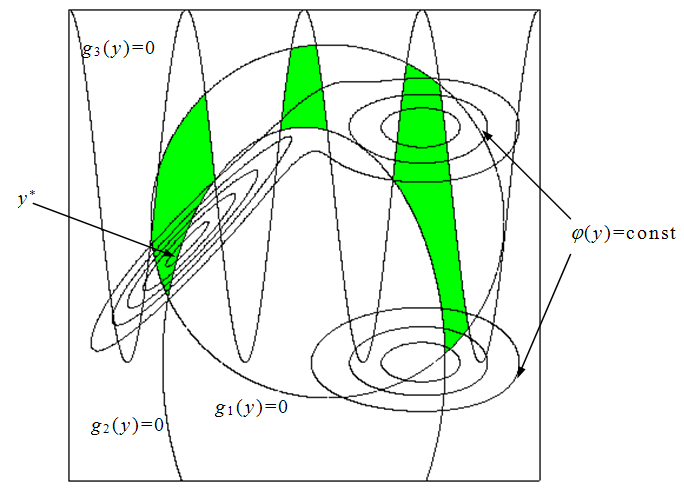
\includegraphics[width=0.7\linewidth]{figures/figure1_1.png}
\caption{Example of a global optimization problem with disconnected admissible domain}
\label{1_fig_1}    
\end{figure}

The set of the points satisfying the first constraint represents a circle with the boundary defined by the equation $g_1(y_1,y_2)=0$. The points satisfying the second constraint are located outside an ellipse defined by the equation $g_2(y_1,y_2)=0$. The points satisfying the third constraint are below the sinusoid $g_3(y_1,y_2)=0$. Thus, the feasible domain is disconnect and consists of three non-convex subdomains (the feasible domain is dark in Fig.~\ref{1_fig_1}). The global minimum $\varphi(y_1^*,y_2^*)=-1.489$  is achieved at the point $(y_1^*,y_2^*)$  = (0.942, 0.944).

\section{Numerical optimization methods}
\label{sec:1_2}

\subsection {Concept of algorithm. Sequential scheme}
\label {subsec:1.2.1}

Having stated the minimization problem, we now must answer the principal question: how to solve it?

The classical approach of the mathematical analysis suggests the following procedure for the analytical solution of the problem. Let us consider the one-dimensional case and assume that $\varphi(y)$ is a single argument function, which is piecewise smooth over the interval $[a,b]$. Then, the minimum of $\varphi(y)$ in $[a,b]$ can be achieved only at the points, where the derivative $\varphi'(y)=0$ , or where the derivative is discontinuous, or at the boundary points. Therefore, it is necessary to find all these points and to select from them the point with the lowest value. In other words, in order to solve the problem by this method, the following requirements should be satisfied:
\begin{enumerate}
\item{it is necessary to know the analytical formula for the function;}
\item{the function should be piecewise smooth;}
\item{the calculation of the derivative should be possible;}
\item{it is necessary to solve the equation $\varphi'(y)=0$;}
\item{the information on the derivative discontinuity points or a method for finding these ones are required.}
\end{enumerate}

Unfortunately, these requirements are fulfilled rarely. In the typical cases, the function $\varphi(y)$ is defined algorithmically, i.e., in the form of some calculation scheme, when one can calculate the value of $\varphi(y)$ at a given point y only (black-box function). In this case, the analytical investigation methods are unsuitable. Note that even if the function is defined analytically and if the derivative calculation is possible the initial problem (\ref{eq:6}) is reduced to the problem of finding all the derivative roots, the difficulty of which is comparable with the minimization problem.

The limited applicability of the analytical methods has caused the development and wide application of \textit {the numerical methods (algorithms)} for solving the optimization problems. Various definitions of the numerical optimization method have been given by many authors. The consideration of the method as an iteration procedure, which calculates certain characteristics of the minimized function at some points of the search domain is a common feature of all formulations. The calculated characteristics can include the value of the objective function, its gradient, the second derivatives matrix, etc. Let us denote the calculation of the function characteristics at a point as \textit {a search trial} and the set of the values of the function characteristics as \textit {a trial result}.

Hereinafter we will consider the function value at the trial point as the trial result. If an algorithm is executed on a single processor computer, the computing scheme of the algorithm consists of a series of operations executed sequentially, and all the trials are performed sequentially, i.e., we deal with a pure sequential numerical method. 

Let us give a formal definition of sequential optimization algorithm based on the methodology of the theory of operations research, or, more general, on the computational model for solving the problem (\ref{eq:6}). The generalization of this model onto the parallel computing case will be given in Subsect. \ref{subsec:1.2.2}

The development of a computational model presupposes an availability of some a priori information on the problem to be solved (before the beginning of the computations). This information could be obtained from the physical meaning of the problem or description of the properties of the model-based object. This information can include such properties of $\varphi(y)$ as continuity, smoothness, monotonicity, convexity, etc. The available information provides the researcher with the basis to attribute the problem (in our case, the function $\varphi(y)$ to a specific set (or class) $\Phi$. After the class $\Phi$ has been identified, the information known to the researcher a priori consists in the knowledge that the problem belongs to the class $\Phi$.

The selection of an \textit {optimization algorithm} (method for solving  the optimization problem) is the next important step in the computational model development. In the most general form, a numerical method $s$ for solving the problem from the class $\Phi$ is a set  (tuple) (\cite{1_StrMonRus})
\begin{equation}
\label{eq:11}
s=\left\langle \{G_k\},\{E_k\},\{H_k\}\right\rangle
\end{equation}
where 

-  $\{G_k\}$	  is a set of functionals defining the rules for the trial points selection \textit {(algorithm's decision rules)}, $k=1,2,\ldots$ ;

-  $\{E_k\}$	  is a set of functionals defining the rules of constructing the approximate solution (the estimate of extremum), $k=1,2,\ldots$ ;

-  $\{H_k\}$	  is a set of functionals defining the rules of stopping the computational process,  $k=1,2,\ldots$.

The order of the trial execution or the computational scheme of the algorithm   can be realized in accordance with the following steps.

\begin{description}[\textbf{Step 1}]
\item[\textbf{Step 1}]{The point 
\begin{equation}
\label{eq:12}
y^1=G_1(\Phi\in Q)
\end{equation}
is selected as the first trial coordinate and the trial counter $k=1$ .}
\item[\textbf{Step 2}]{Assume the point of the $k$-th trial $y^k\in Q$  $(k\geq 1)$ has been selected. The value of the function $z^k=\varphi(y^k)$  is computed. Afterwards there is the following \textit {search (a posteriori) information} about the function $\varphi(y)$:
\begin{equation}
\label{eq:13}
\omega_k=\{(y^1,z^1),(y^2,z^2),\ldots ,(y^k,z^k)\}.
\end{equation}
This information allows reducing the class, which the function  $\varphi(y)$ belongs to, up to the set
\begin{equation}
\label{eq:14}
\Phi(\omega_k)=\{\psi\in\Phi:\psi(y^i)=z^i,1\leq i \leq k\}.
\end{equation}
}
\item[\textbf{Step 3}]{The current estimate 
\begin{equation}
\label{eq:15}
e^k=E_k(\Phi,\omega_k)
\end{equation}
of the extremum sought (approximate solution) is determined.}
\item[\textbf{Step 4}]{The next trial point 
\begin{equation}
\label{eq:16}
y^{k+1}=G_{k+1}(\Phi,\omega_k)
\end{equation}
is computed.}
\item[\textbf{Step 5}]{The number 
\begin{equation}
\label{eq:17}
h^k=H_k(\Phi,\omega_k,y^{k+1})\in \{0,1\}
\end{equation}
taking one of two possible values: 0 or 1 is determined. If $h^k=1$ the trial counter $k$ is increased by 1, and the return to the Step 2 of the scheme is carried out. If $h^k=0$ the computations are terminated, and the estimate $e^k$  is taken as the problem solution.}
\end{description}

The general computation model has been described. 

\example {Let us consider the simplest method of solving a one-dimensional problem (\ref{eq:6}) within an interval $[a,b]$, namely, the method of scanning  the function values in the nodes of a regular grid. The method consists in the partitioning of the search interval $[a,b]$ into $q$ equal parts. The function values are calculated at the points (nodes) of the partitioning, including the ends of the search interval. The lowest calculated value (and its coordinate, if it is required by the problem statement) is considered to be the solution of the problem. }

The computability of the function at any point of the search domain is sufficient for the applicability of the method. So, the class of the functions defined over the interval $[a,b]$ and being computable at every point of the interval could be considered as the a priori known class $\Phi$. 

For this method
\begin{displaymath}
G_1(\Phi)=a, G_{k=1}(\Phi,\omega_k)=a+k\frac{b-a}{q}, k\geq 1,
\end{displaymath}
\begin{displaymath}
  H_k(\Phi,\omega_k) =
  \begin{cases}
    0, & k > q, \\
    1, & k \leq q,
  \end{cases}
\end{displaymath}
\begin{equation}
\label{eq:18}
e^k=\varphi_k^*,
\end{equation}
where
\begin{equation}
\label{eq:19}
\varphi_k^*=\min_{1\leq i\leq k} \varphi(y^i),
\end{equation}
or
\begin{displaymath}
e^k=(\varphi_k^*,y_k^*),
\end{displaymath}
where 
\begin{displaymath}
%\label{eq:19}
y_k^*=\arg \min_{1\leq i\leq k} \varphi(y^i).
\end{displaymath}


\subsection {Parallel optimization algorithms}
\label {subsec:1.2.2}
The computational scheme (\ref{eq:12})--(\ref{eq:17}) implies  the sequential execution of all the algorithm steps, that can be provided by the single processor computers. But if a multiprocessor computer is available, a parallelization of the computational scheme and, therefore, an acceleration of the optimization process can be realized. The parallelization of optimization methods could be done in several ways. It is possible to parallelize, in the first place, the calculation of the objective function, secondly, the implementation of the rules $G_k,E_k,H_k$ , and, finally, the scheme (\ref{eq:12})--(\ref{eq:17}) providing simultaneous execution of several trials. However, the parallelization of the objective function describing the optimized object is specific for different objective function models, and as a matter of fact, cannot be related to the general optimization scheme. The parallelization of the functionals  $G_k,E_k,H_k$ depends essentially on the class of algorithms. Besides, often these functionals are rather simple, and their parallelization is just of no use. Therefore, Therefore, the subject of the consideration in the present subsection  is the design of some \textit {fundamental principles} for a parallel execution of trials.  Let us use the term \textit {iteration} for the simultaneous (parallel) execution of several trials (each trial is executed by a separate processor). Let us denote the number of trials during the $n$-th iteration as $p(n)$ , and the total number of trials executed during all $n$ iterations as $k(n)$ . In other words, we assume that we have  $p$  processors at our disposal while executing the $n$-th iteration. Actually, the number of processors employed can be different for different iterations. 

Let us consider the synchronous variant of the parallelization, where the transition to the next iteration is performed after full termination of the current one, i.e., after completing the last trial of the current iteration. In this case, it is obvious that $k(n)=p(1)+\ldots + p(n), \; n\geq 1$.  Let us denote the vector of the trial coordinates at the $n$-th iteration as $u(n)$ , i.e.,
\begin{displaymath}
u(n)=(y^{k(n-1)+1},\ldots ,y^{k(n)}) .
\end{displaymath}
and the first $j$ coordinates of the vector $u(n)$  as $u_j(n)$ , i.e., 
\begin{displaymath}
u(n)=(y^{k(n-1)+1},\ldots ,y^{k(n-1)+j}),\ 1\leq j\leq p(n) .
\end{displaymath}

Then, the general computational scheme of a synchronous parallel optimization algorithm can be written as follows.

\paragraph{\textbf{Synchronous parallel algorithm scheme}}
\begin{description}[\textbf{Step 1}]
\item[\textbf{Step 1}]{Set the iteration number $n=1$  and the initial number of trials $k(0)=0$ . Select $p(1)$ points of the first iteration  
\begin{equation}
\label{eq:20}
y^1=G_1(\Phi\in Q),y^i=G_i(\Phi,u_{i-1}(1))\in Q,\ 2\leq i\leq p(1)
\end{equation}
and assign the number of trials $k(1)=p(1)$.}
\item[\textbf{Step 2}]{Assume that the points of the $n$th iteration $u(n),\ n\geq 1,$ , have been obtained. The computations of the objective function values $z^j=\varphi(y^j),\ k(n-1)+1\leq j\leq k(n)$, are executed (each value is computed by a separate processor). After computing all the values there is the following search information on the function $\varphi(y)$ (\textit{a posteriori information}):
\begin{equation}
\label{eq:21}
\omega_k=\omega_{k(n)}=\{(y^1,z^1),(y^2,z^2),\ldots ,(y^{k(n)},z^{k(n)})\}.
\end{equation}
As before, the new information (\ref{eq:21}) allows one to reduce the class, which the function $\varphi(y)$ belongs to, up to the set   
\begin{equation}
\label{eq:22}
\Phi(\omega_{k(n)})=\{\psi\in\Phi:\psi(y^i)=z^i,1\leq i \leq k(n)\}.
\end{equation}
}
\item[\textbf{Step 3}]{After completing all the trials within the current iteration, the estimate of the extremum (an approximate solution) is formed:  
\begin{equation}
\label{eq:23}
e^{k(n)}=E_{k(n)}(\Phi,\omega_{k(n)}).
\end{equation}
}
\item[\textbf{Step 4}]{$p(n+1)$   coordinates of the trials of the $n+1$-th iteration are computed:
\begin{equation}
\label{eq:24}
\begin{gathered}
y^{k(n)+1}=G_{k(n)+1}(\Phi,\omega_{k(n)}) \\
y^i=G_i(\Phi,\omega_{k(n)},u_{i-1}(k(n+1))
\end{gathered}
\end{equation}
and the number of the search trials $k(n+1)=k(n)+p(n+1)$  is set.}
\item[\textbf{Step 5}]{The number 
\begin{equation}
\label{eq:25}
h^{k(n)}=H_{k(n)}(\Phi,\omega_{k(n)},u_{n+1})\in \{0,1\}
\end{equation}
taking one of two possible values: 0 or 1 is determined. If $h^{k(n)}=1$ the iteration counter $k$ is incremented ($n=n+1$), and the return to the Step 2 of the scheme is carried out. If $h^{k(n)}=0$ the  iterations are completed, and the estimate $e^{k(n)}$  is taken as the (approximate) problem solution.}
\end{description}
\note {In the proposed scheme it is assumed implicitly, that the numbers   of the processors involved into the execution of a particular step of the algorithm  are known a priori for all iterations. At the same time, the scheme can be easily supplemented with a processor number selection rule in dependence on the current search state, if to introduce a functional $P_n(\Phi,\omega_{k(n-1)})$  such that}
\begin{displaymath}
p(n)= P_n(\Phi,\omega_{k(n-1)}).
\end{displaymath}

Then, Step 4 of the computational scheme can be written as follows. 
\begin{description}[\textbf{Step 4}]
\item[\textbf{Step 4}]{The number of processors required for the execution of the  $(n+1)$-th iteration 
\begin{displaymath}
p(n+1)= P_{n+1}(\Phi,\omega_{k(n)}).
\end{displaymath}
is determined and $p(n+1)$  trial coordinates of the current iteration are calculated according to (\ref{eq:24}).}
\end{description}

Let us consider again the method of scanning  a function $\varphi(y)$ in the nodes of a regular grid to illustrate a parallel algorithm. Let us assume for simplicity that the number of processors $p$ is the same for all iterations, that the number of nodes $q>p$  and is divisible by $p$. Then, the decision rules $G(\bullet )$  in the expressions (\ref{eq:20}) and (\ref{eq:24})  obviously take the form 
\begin{displaymath}
G(\bullet )=a+(i-1)\frac{b-a}{q},\ 1\leq i\leq k(n)+1,
\end{displaymath}
and the estimate of extremum and the condition of termination remain the same to those in the sequential prototype. 

The synchronous scheme considered here has a drawback that the processors completed their trails within current iteration earlier than other ones, stay idle waiting for the completion of the iteration. Let us consider the computational scheme of an \textit{asynchronous} parallel optimization algorithm, which is free from this disadvantage. In the asynchronous algorithm the iterations become distributed in time. Therefore, it is convenient to deal with the number of trials $k$. In this connection, let us introduce a set of completed trials  $w(k)=\{w_1,w_2,\ldots,w_k\}$  and a set  of coordinates $v(k)=\{v_1,v_2,\ldots,v_{p(k)}\}$ , at which new trials are executed after completing the preceding $k$ trials. Here $p(k)$ is the number of processors executing the current trials, and $w_j=y^{i_j},\ 1\leq j\leq k,\ v_s=y^{i_s},\ 1\leq s\leq p(k), 1\leq i_j,i_s \leq k+p(k)$ . It is obvious, that $w(k)\cup v(k)=\{y^1,\ldots,y^k,\ldots,y^{k+p(k)}\}$ .

Let us assume for simplicity, that we have  $p\geq 2$  processors at our disposal for execution of the algorithm, and this number remains constant in the course of optimization. A variant of the computational scheme with a different number of processors for different search steps can be obtained easily by generalization of the proposed asynchronous scheme consisting in the following.
\paragraph{Asynchronous parallel algorithm scheme}
\begin{description}[\textbf{Step 1}]
\item[\textbf{Step 1}]{First $p$ points of initial trials are selected according to the decision rules $G_i(\bullet ),\ 1\leq i\leq p$ :  
\begin{equation}
\label{eq:26}
\begin{gathered}
y^1=G_1(\Phi\in Q), \\
y^i=G_i(\Phi,y^1,\ldots,y^{i-1)}\in Q,\ 2\leq i\leq p,
\end{gathered}
\end{equation}
the vector $v(0)$  with the components $v_i=y^i,\;1\leq i\leq p$, is formed, and the number of trials $k=0$ is set.}
\item[\textbf{Step 2}]{Wait for the completion of trials by one or several processors. Assume that $1\leq \pi=\pi(k)\leq p$  processors have completed the computation of the function values $z^{i_j}=\varphi(y^{i_j})$  at the points $y^{i_1},\ldots,y^{i_\pi}, y^{i_j}\in v(k),\ 1\leq j\leq \pi$. Then, assign $k=k+\pi$, form the set $w(k)=w(k-\pi)\bigcup \{y^{i_1},\ldots,y^{i_\pi}\}$  and the set $v(k)$ removing from the set $v(k-\pi)$  points $y^{i_1},\ldots,y^{i_\pi}$ . Afterwards there is the following search information on the function $\varphi(y)$ \textit{a posteriori}:
\begin{equation}
\label{eq:27}
\omega_k=\{(y^{i_1},z^{i_1}),(y^{i_2},z^{i_2}),\ldots ,(y^{i_k},z^{i_k}\}.
\end{equation}
where  $y^{i_s}\in w(k),z^{i_s}=\varphi(y^{i_s}),\;1\leq s\leq k$.
}
\item[\textbf{Step 3}]{The current estimate (approximate solution) of the extremum is determined as  
\begin{equation}
\label{eq:28}
e^k=E_k(\Phi,\omega_k).
\end{equation}
}
\item[\textbf{Step 4}]{
\begin{equation}
\label{eq:29}
\begin{gathered}
y^{k+1}=G_{k+1}(\Phi,\omega_{k}) \\
y^i=G_i(\Phi,\omega_k,y^{k+1},\ldots,y^{k+i-1}),\;k+2\leq i\leq k+\pi,
\end{gathered}
\end{equation}
are computed and added to the set $v(k)$.} 
\item[\textbf{Step 5}]{The number 
\begin{equation}
\label{eq:30}
h^k=H_k(\Phi,\omega_k,y^{k+1},\ldots,y^{k+\pi})\in \{0,1\}
\end{equation}
taking one of two possible values: 0 or 1 is computed. If $h^k=1$, switching to Step 2 of the current scheme is carried out. If $h^k=0$, the computations should be completed and the current estimate $e^k$  is taken as the problem solution.}
\end{description}

Some examples of both the synchronous and asynchronous optimization algorithms are presented in the next chapters.
\subsection {Convergence and estimates of extremum}
\label {subsec:1.2.3}
Thus, when solving a minimization problem for a function  $\varphi(y)$ any search method generates a sequence of trial coordinates (or just the trial sequence) $\{y^k\}=y^1,y^2,\ldots,y^k,\ldots$  (where $y^k$   is the coordinate of the $k$-th trial) as well as a sequence of trial results $\{z^k\}=z^1,z^2,\ldots,z^k,\ldots$ . Remind, that as trial results we consider the objective function values, i.e., $z^i=\varphi(y^i),\;i=1,2,\ldots$ .    

The behavior of the method is determined via the properties of sequences  $\{y^k\}$ and  $\{z^k\}$. Therefore, the investigation of the search method could be carried out by means of a study of trial sequences which it generates. 

Thereby, let us ask the question: what requirements should be imposed to trial sequences of a numerical optimization method? Of course, the main requirement is that execution of the trials at the points $\{y^k\}$  with the trial results $\{z^k\}$  could provide a solution of the problem, i.e., finding the solution corresponding to the selected problem statement. At the same time, since a computer can execute a finite number of trials only, it is desirable to obtain the exact solution after constructing a finite sequence $\{y^k\}$. Therefore,  an asymptotically exact assessment is interesting often, and an infinite trial sequence is considered (in the introduced  optimization method models in (\ref{eq:17}) , (\ref{eq:25}), (\ref{eq:30}) $H_k=1$  for any $k\geq1$, i.e., in fact, the termination criterion is absent). This sequence is required to converge to the exact problem solution. Since in the problem statements $B-D$ the desired solution may include several minimum points, we will understand the convergence of a method in the scope of the following definition.
\begin{definition} 
\label{def:1_4}
The trial sequence $\{y^k\}$  converges to the solution of the problem (\ref{eq:6}) defined by the corresponding problem statement, if:
\begin{enumerate}
\item{it includes a subsequence  $\{\bar{y}^k\}$, for which $\lim_{k \to \infty}\bar{y}^k=\varphi^*$;}
\item{in the case when the solution includes one or several minimum points, for each such point there exists a subsequence of the sequence $\{y^k\}$  converging to it.}
\end{enumerate}
\end{definition}
Trial sequence converging to the exact solution of the problem statement $Z \in \{A,B,C,D,E\}$ is called the minimizing sequence for the problem statement $Z$ or $Z$-minimizing sequence. The term «minimizing sequence» was introduced in \cite{1_Vasiliev} and corresponds to the concept of $A$-minimizing sequence.

Now we would like to pay the reader’s attention to the following important aspect. The property of convergence in the theory of the extremum search methods attracts significant attention, since the asymptotics provides a potential possibility to obtain the exact solution with any predefined accuracy after a finite number of trials. However, this possibility itself is not sufficient for the practical implementation of the methods. In addition, it is necessary to know how to determine a proximity measure of the obtained approximate solution to the exact one, i.e., how to estimate the error of the problem solution using the finite number of trials.

Let us consider the following simple example. Let the class $\Phi$ consist of the continuous one-dimensional functions, defined over the interval $Q=[a,b]$, i.e., it is known a priori that the minimized function $\varphi(y)$ is continuous in the domain $Q$. Assume that the values of the function $\varphi(y)$ are calculated in a finite number of points   What is it possible to say about the coordinate of the global minimum after that? Whatever points $y^1,y^2,\ldots,y^k$  and values $z^1,z^2,\ldots,z^k$ , were obtained after $k$  trials, for any point $y^*\in Q (y^*\notin \{y^1,y^2,\ldots,y^k\})$   a continuous function passing through the points $(y^i,z^i),1\leq i\leq k$,  i.e., belonging to the class $\Phi(\omega_k$ from (\ref{eq:14}) and providing the global minimum at the point $y^*$  with any predefined value
\begin{displaymath}
\varphi^*<\min_{1\leq i\leq k} z^i 
\end{displaymath}
can be built always. For example, an interpolation polynomial of the $k$-th power, passing through the points  $(y^i,z^i),1\leq i\leq k,$ and the point $(y^*,\varphi^*)$, could be taken as such function.

All the above means that no conclusions on the position of the global minimum point can be drawn after any  finite number of trials. Similarly, the only conclusion on the value $\varphi^*$  of the global minimum could be as follows:
\begin{displaymath}
\varphi^*\leq \varphi_k^*, 
\end{displaymath}
where $\varphi_k^*$  is determined by (\ref{eq:19}). Therefore, it is impossible to estimate the value 
\begin{displaymath}
\epsilon_k=\left|\varphi^*-\varphi_k^*\right|, 
\end{displaymath}
i.e., the accuracy of the program solution.

The possibility to obtain the estimates of the extremum based on a finite number of trials depends on the properties of the function class, which the minimized function belongs to, or, in other words, on the information about the function $\varphi(y)$ known a priori. In fact, only two broad classed of the functions allow building such estimates: the class of one-dimensional unimodal functions and the class of the functions satisfying Lipschitz condition (in the general case of the multidimensional and multiextremal functions).

The availability of the extremum estimates built on the base of a finite (truncated) trial sequence allows (in some cases) formulating and solving the problem of theoretical design of the optimal (in different meanings) optimization methods (see, for example, \cite{1_Kushner, 1_Mockus, 1_StrSergMon2000, 1_Sukharev1971, 1_Sukharev1972, 1_Sukharev1989}) . This interesting problem falls out of the scope of the present paper. However, the availability of the extremum estimates is important for the investigation of the parallelization efficiency of the optimization methods considered in the next chapters.

\section{Multiextremal problems and reduction of complexity}
\label{sec:1_3}
In multiextremal problems the dimension affects the difficulty of solving such problems significantly. For example, for the class of the functions satisfying Lipschitz condition so called «the curse of dimensionality» consisting in the exponential growth of the computational costs with increasing dimensionality takes place. Namely, if $p$ evaluations of the objective function are required to achieve the solution accuracy $\epsilon$ in the one-dimensional case, in the $N$-dimensional problem $\alpha p^N$  trials are required to achieve the same accuracy. Here the coefficient $\alpha$ depends on the objective function, on the feasible domain, and on the method used. 

For particular small classes of the multiextremal problems the computational cost growth rate can be slower than the exponential one. For example, for the separable functions minimized over a hyperinterval $D$ the computational costs grow linearly. This fact demonstrates that increase of the efficiency of optimization methods is possible by a thorough accounting for the a priori known information only. Designing the efficient optimization methods as optimal decision rules based on the minimax or Bayesian approach to the concept of optimal methods of the extremum search within the frameworks of the respective mathematical models can be a form of such accounting. Unfortunately, the problem of building the optimal algorithm for the multidimensional multiextremal functions is  very complicated and connected with solving the problems of the covering theory of the feasible domain (see, for example, \cite{1_Sukharev1971, 1_Sukharev1972, 1_Sukharev1989}).

Another approach to the design of the numerical methods for the analysis of the multidimensional multiextremal problems exploits the idea of \textit{the complexity reduction} where the solution of the initial problem is replaced by solving one or several simpler problems.

One of such reduction schemes is based on the elementary fact that the global extremum is a local one. Hence the clear conclusion follows that in order to find the global optimal solution it is sufficient to find all local minima and to select the lowest of them. In the context of the theoretical approach this construct seems to be a perfect one. However, in practice everything is not so rosy. 
First of all, the following question arises: how to find all local minima? This problem could be solved, if for each local minimum its attraction zone, i.e., such neighborhood of the minimum point, in which the function is unimodal, is known. Then, having positioned the initial search point into this neighborhood, one can find the desired local minimum by some local method. In other words, this scheme implies a subdivision of the search domain into the local minimum attraction zones to be known. However, in practice such information is absent a priori as a rule (even the number of local extrema is unknown usually). Therefore, an additional problem of the starting point selection arises when applying this approach. 

The simplest method consists in the selection of the starting points using the Monte-Carlo method scheme (see, for example, the fundamental monograph \cite{1_ZhigZhil}), i.e., randomly according to some distribution in the search domain (usually, the uniform one) or in using the nodes of a regular grid as the starting points.

The convergence to the global extremum in this method is provided by the fact that if to increase the number of the starting points at least one of them should fall into the global extremum attraction zone since these grids (either regular or random) are built to provide a coverage of the whole search domain with increasing density. However, this scheme has an essential drawback. As a matter of fact, several starting points can fall into the attraction zone of a local minimum, i.e., this particular local minimum will be found several times. Different schemes have been proposed to overcome this disadvantage ( see \cite{BetroSchoen, BoendeRinnooy, 1_Zielinski}). 

The idea of one of them is as follows. First, $L$ base points are selected within the search domain (usually, distributed more or less uniformly). Then, the objective function values are calculated at these points, i.e., actually a rough estimate of the function behavior is performed. Then, the $l<L$  “best” points, i.e., such ones, where the function values are less than at the rest points (at the same time, these “best” points are not too close to each other) are selected from the base points set. These $l$ points serve as the starting points for the local search. There exists a plenty of variants of this scheme. For example, the set of the base points can be modified during the search process: new points can be added to this set. Also, the method of  the point selection may be modified in the course  of the realization of this scheme taking into account the new information obtained, etc. 

There also exist other schemes built on the base of the reduction of a multiextremal problem to solving the local subproblems. The algorithms designed within the framework of this approach have an asymptotic convergence to the global extremum with weak presumptions of the continuity or of some degree of differentiability of the objective function. From the quite strict theoretical point of view, this convergence is provided by such property that any point of the search domain is an accumulation point of the trial sequence   generated by the algorithm and, consequently, for a continuous function
\begin{equation}
\label{eq:31}
\lim_{\tau \to \infty}\min_{1\leq k \leq \tau}{\varphi(y^k)}=\varphi^*.
\end{equation}
In other words, the trial sequences of these methods are everywhere dense in the search domain, i.e., converge in the sense of Definition \ref{def:1_4} to all points within this domain and, consequently, to the global minimum point as well. 

Generally, this character of convergence is too «prodigal», that does not favor the efficiency of the method of this type. Avoiding this drawback is possible only if enough and rather rich a priori known information on the problem is available (like the data on the attraction zones). Such information is rather rarely available in practice and sometimes could be obtained for simple multiextremal problems with a few number of extrema only. For such problems this approach is quite efficient. However, for the essentially multiextremal problems the application of reduction to the local minimum problems is not successful, as a rule. At the same time, the methods of this class are parallelized rather easily, but the everywhere dense convergence (\ref{eq:31}) can results in a large number of redundant trials. 

Another approach based on the idea of dimensionality reduction, i.e., on building the schemes, where solving a multidimensional problem is reduced to solving one or several one-dimensional subproblems is more fruitful as compared with the reduction to the local problems. The following two efficient schemes of this kind are known:
\begin{enumerate}
\item{the nested optimization scheme  of optimization \cite{1_CarrHowe, 1_Evtushenko, 1_GerGriIsr, 1_GerGriGer, 1_GriIsrAIP, 1_GriIsrSerg, 1_GriIsrCEUR, 1_Piyavskij, 1_SergGriJCAA, 1_ShiOlaf, 1_StrMonRus, 1_StrSergMon2000, 1_vanDam},}
\item{the reduction of dimensionality based on the curves filling the space (Peano-type curves) \cite{1_Butz, 1_Goertzel, 1_HimOliPet, 1_LeraSergCNSNS, 1_LeraSergANM, 1_SergStrLeraMonogr, 1_StrMonRus,1_StrSergMon2000}.}
\end{enumerate}
The \textit{nested optimization scheme} of dimensionality reduction replaces solving the problem (\ref{eq:8})--(\ref{eq:10}) with solving a family of recursively nested one-dimensional subproblems, in which every evaluation of the objective function within a one-dimensional subproblem consists in solving a new one-dimensional subproblem of the next level of the recursion except the last one, where the value of the initial multidimensional objective function is calculated. 

The second scheme is the dimensionality reduction based on the Peano-type curves. It is based on the well known fundamental fact, according to which the $N$-dimensional hyperparallelepiped (\ref{eq:10}) and the interval $[0,1]$ of the real axis are the equinumerous sets, and the interval $[0,1]$ can be mapped onto the parallelepiped (\ref{eq:10}) , unambiguously and continuously \cite{1_SergStrLeraMonogr, 1_StrSergMon2000}. The representations of this kind are usually called \textit{Peano-type curves} or \textit{evolvents}. 

Let $y(x),[\in [0,\:1]$  be a Peano-type curve, and the function  $\varphi(y)$ from (\ref{eq:8}) be continuous. Then because of the continuity of  $\varphi(y)$, $y(x)$ and owing to the relation
\begin{displaymath}
D=\{y(x):x\in [0,\:1]\} 
\end{displaymath}
we have the equality
\begin{displaymath}
\min_{y\in D}\varphi(y)=\min_{x\in [0,\;1]}\varphi(y(x)) 
\end{displaymath}
i.e., solving the multidimensional problem of minimization of $\varphi(y)$ over the hyperparallelepiped $D$ is reduced to the minimization of the one-dimensional function $\varphi(y(x))$ over the interval $[0,\;1]$.

The consideration and justification of the algorithms based on the nested optimization scheme and on the dimensionality reduction schemes using Peano-type curves is the major subject of the next chapters. 
% 
\begin{thebibliography}{99.}
\bibitem{BetroSchoen} Betro, B., Schoen, F.: Sequential stopping rules for the multistart algorithm in global optimisation. Math. Program. \textbf{38}(3), 271--286 (1987)
\bibitem{BoendeRinnooy}	Boender, C.G.E, Rinnooy Kan, A.H.G.: Bayesian stopping rules for multistart global optimization methods. Math. Program. \textbf{37}(1), 59--80 (1987)
\bibitem{1_Butz}	Butz, A.R. Space-Filling Curves and Mathematical Programming.: Inform. Control \textbf{12}, 314--330 (1968)
\bibitem{1_CarrHowe}	Carr, C.R., Howe, C.W.: Quantitative Decision Procedures in Management and Economic: Deterministic Theory and Applications. McGraw-Hill, New York (1964)
\bibitem{1_Evtushenko}	Evtushenko, Yu.G.: Numerical Optimization Techniques. Translation Series in Mathematics and Engineering. Optimization Software  Inc., Publication Division, New York (1985)
\bibitem{1_FloudasPardalos} Floudas, C.A., Pardalos, P.M.: State of the Art in Global Optimization. Kluwer Academic Publishers, Dordrecht (1996)
\bibitem{1_GerGriIsr} Gergel, V.,  Grishagin, V., Israfilov, R.: Local tuning in nested scheme of global optimization, Procedia Computer Science \textbf{51}, 865--874 (2015) 
\bibitem{1_GerGriGer}	Gergel, V., Grishagin, V., Gergel, A.: Adaptive nested optimization scheme for multidimensional global search, J. Glob. Opt. \textbf{66}, 35–51 (2016).
\bibitem{1_Goertzel}	Goertzel, B.: Global Optimization with Space-Filling Curves. Appl. Math. Lett. 12, 133--135 (1999)
\bibitem{1_GriIsrAIP}	Grishagin, V.A., Israfilov, R.A.: Global search acceleration in the nested optimization scheme. AIP Conf. Proc. \textbf{1738}, 400010 (2016)
\bibitem{1_GriIsrSerg}	Grishagin, V.,  Israfilov, R., Sergeyev, Y.: Convergence conditions and numerical comparison of global optimization methods based on dimensionality reduction schemes. Appl. Math.  Comput. (2017) doi:10.1016/j.amc.2017.06.036
\bibitem{1_GriIsrCEUR}Grishagin, V.A., Israfilov, R.A.: Multidimensional Constrained Global Optimization in Domains with Computable Boundaries. CEUR Workshop Proceedings 1513, 75--84 (2015)
\bibitem{1_HimOliPet}	Hime, A.E., Oliveira Jr., H.A., Petraglia, A.: Global Optimization Using Space-Filling Curves and Measure-Preserving Transformations. Soft Computing in Industrial Applications \textbf{96}, 121--130 (2011)
\bibitem{1_Himmelblau}	Himmelblau, D.M.: Applied Nonlinear Programming. McGraw-Hill, New York (1972)
\bibitem{1_HorstPardalos}	Horst, R., Pardalos, P.M.: Handbook of Global Optimization. Kluwer Academic Publishers, Dordrecht (1995)
\bibitem{1_HorstTuy}	Horst, R., Tuy, H.: Global Optimization:Deterministic Approaches. Springer-Verlag, Berlin (1990) (2nd edn., 1993; 3rd edn., 1996)
\bibitem{1_Kushner}	Kushner, H.J.: A new method of locating the maximum point of an arbitrary multipeak curve in the presence of noise. Transactions of ASME, Ser. D. Journal of Basic Engineering \textbf{86}, 97--106 (1964)
\bibitem{1_LeraSergCNSNS}	Lera, D., Sergeyev, Y.D.: Deterministic global optimization using space-filling curves and multiple estimates of Lipschitz and H{\"o}lder constants. Communications in Nonlinear Science and Numerical Simulation \textbf{23}, 328--342 (2015)
\bibitem{1_LeraSergANM}	Lera, D., Sergeyev, Y.D.: Lipschitz and H{\"o}lder global optimization using space-filling curves. Applied Numerical Mathematics \textbf{60}, 115--129 (2010) 
\bibitem{1_McCormick}	McCormick, G.P.: Nonlinear Programming: Theory, Algorithms and Applications. John Wiley and Sons, New York (1988)
\bibitem{1_Mockus}	Mockus, J.: Bayesian Approach to Global Optimization. Kluwer Academic Publishers, Dordrecht (1988) 
\bibitem{1_Pinter}	Pint{\'e}r, J.D.: Global Optimization in Action.: Kluwer Academic Publishers, Dordrecht (1996) 
\bibitem{1_Piyavskij}	Piyavskij, S.A.: An Algorithm for Finding the Absolute Extremum of a Function. USSR Comput. Math. Math. Phys. \textbf{12}(4), 57--67 (1972)
\bibitem{1_SergGriJCAA}	Sergeyev, Y.D., Grishagin, V.A.: Parallel Asynchronous Global Search and the Nested Optimization Scheme. J. Comp. Analysis Appl. \textbf{3}, 123--145 (2001)
\bibitem{1_SergKvasMonogr}	Sergeyev, Y.D., Kvasov, D.E.: Deterministic Global Optimization: Diagonal Approach Briefly. Springer-Verlag, New York (2017)
\bibitem{1_SergStrLeraMonogr}	Sergeyev, Y.D., Strongin, R.G., Lera, D.: Introduction to Global Optimization Exploiting Space-Filling Curves. Springer (2013)
\bibitem{1_ShiOlaf}   Shi, L., {\'O}lafsson, S.: Nested Partitions Method for Global Optimization. Operations Research \textbf{48}, 390--407 (2000)
\bibitem{1_StrMonRus}	Strongin, R.G.: Numerical Methods in Multiextremal Problems (Information-Statistical Algorithms). Nauka, Moscow (1978). In Russian
\bibitem{1_StrSergMon2000} Strongin, R.G., Sergeyev, Y.D.: Global Optimization with Non-Convex Constraints. Sequential and Parallel Algorithms. Kluwer Academic Publishers, Dordrecht (2000) 
\bibitem{1_Sukharev1971}	Sukharev, A.G.: Optimal strategies of the search for an extremum. USSR Comput. Math.Math. Phys. \textbf{11}(4), 119–137 (1971)
\bibitem{1_Sukharev1972}	Sukharev, A.G.: Best sequential search strategies for finding an extremum. USSR Comput. Math. Math. Phys. \textbf{12}(1), 39–59 (1972)
\bibitem{1_Sukharev1989}	Sukharev, A.G.: Minimax Algorithms in Problems of Numerical Analysis. Nauka, Moscow (1989). In Russian
\bibitem{1_vanDam}	van Dam, E.R., Husslage, B., Hertog, D. One-dimensional Nested Maximin Designs. J. Glob. Opt. \textbf{46}, 287--306 (2010)
\bibitem{1_Vasiliev}	Vasiliev, F.P. Numerical Methods for Solving Extremal Problems. Nauka, Moscow (1988). In Russian
\bibitem{1_ZhigZhil} Zhigljavsky, A.A., $\check{Z}$ilinskas, A.: Stochastic Global Optimization. Springer, New York. (2008)
\bibitem{1_Zielinski}	Zieli{\'n}ski, R.: A statistical estimate of the structure of multi-extremal problems. Math. Program. \textbf{21}(1), 348--356 (1981)

\end{thebibliography}
%%%%%%%%%%%%%%%%%%%%%%%%% referenc.tex %%%%%%%%%%%%%%%%%%%%%
% sample references
% 
% Use this file as a template for your own input.
%
%%%%%%%%%%%%%%%%%%%%%%%% Springer%%%%%%%%%%%%%%%%%%%%%%%%%%
%
% BibTeX users please use
% \bibliographystyle{}
% \bibliography{}
%
\biblstarthook{References may be \textit{cited} in the text either by number (preferred) or by author/year.\footnote{Make sure that all references from the list are cited in the text. Those not cited should be moved to a separate \textit{Further Reading} section or chapter.} The reference list should ideally be \textit{sorted} in alphabetical order -- even if reference numbers are used for the their citation in the text. If there are several works by the same author, the following order should be used: 
\begin{enumerate}
\item all works by the author alone, ordered chronologically by year of publication
\item all works by the author with a coauthor, ordered alphabetically by coauthor
\item all works by the author with several coauthors, ordered chronologically by year of publication.
\end{enumerate}
The \textit{styling} of references\footnote{Always use the standard abbreviation of a journal's name according to the ISSN \textit{List of Title Word Abbreviations}, see \url{http://www.issn.org/en/node/344}} depends on the subject of your book:
\begin{itemize}
\item The \textit{two} recommended styles for references in books on \textit{mathematical, physical, statistical and computer sciences} are depicted in ~\cite{science-contrib, science-online, science-mono, science-journal, science-DOI} and ~\cite{phys-online, phys-mono, phys-journal, phys-DOI, phys-contrib}.
\item Examples of the most commonly used reference style in books on \textit{Psychology, Social Sciences} are~\cite{psysoc-mono, psysoc-online,psysoc-journal, psysoc-contrib, psysoc-DOI}.
\item Examples for references in books on \textit{Humanities, Linguistics, Philosophy} are~\cite{humlinphil-journal, humlinphil-contrib, humlinphil-mono, humlinphil-online, humlinphil-DOI}.
\item Examples of the basic Springer style used in publications on a wide range of subjects such as \textit{Computer Science, Economics, Engineering, Geosciences, Life Sciences, Medicine, Biomedicine} are ~\cite{basic-contrib, basic-online, basic-journal, basic-DOI, basic-mono}. 
\end{itemize}
}

\begin{thebibliography}{99.}%
% and use \bibitem to create references.
%
% Use the following syntax and markup for your references if 
% the subject of your book is from the field 
% "Mathematics, Physics, Statistics, Computer Science"
%
% Contribution 
\bibitem{science-contrib} Broy, M.: Software engineering --- from auxiliary to key technologies. In: Broy, M., Dener, E. (eds.) Software Pioneers, pp. 10-13. Springer, Heidelberg (2002)
%
% Online Document
\bibitem{science-online} Dod, J.: Effective substances. In: The Dictionary of Substances and Their Effects. Royal Society of Chemistry (1999) Available via DIALOG. \\
\url{http://www.rsc.org/dose/title of subordinate document. Cited 15 Jan 1999}
%
% Monograph
\bibitem{science-mono} Geddes, K.O., Czapor, S.R., Labahn, G.: Algorithms for Computer Algebra. Kluwer, Boston (1992) 
%
% Journal article
\bibitem{science-journal} Hamburger, C.: Quasimonotonicity, regularity and duality for nonlinear systems of partial differential equations. Ann. Mat. Pura. Appl. \textbf{169}, 321--354 (1995)
%
% Journal article by DOI
\bibitem{science-DOI} Slifka, M.K., Whitton, J.L.: Clinical implications of dysregulated cytokine production. J. Mol. Med. (2000) doi: 10.1007/s001090000086 
%
\bigskip

% Use the following (APS) syntax and markup for your references if 
% the subject of your book is from the field 
% "Mathematics, Physics, Statistics, Computer Science"
%
% Online Document
\bibitem{phys-online} J. Dod, in \textit{The Dictionary of Substances and Their Effects}, Royal Society of Chemistry. (Available via DIALOG, 1999), 
\url{http://www.rsc.org/dose/title of subordinate document. Cited 15 Jan 1999}
%
% Monograph
\bibitem{phys-mono} H. Ibach, H. L\"uth, \textit{Solid-State Physics}, 2nd edn. (Springer, New York, 1996), pp. 45-56 
%
% Journal article
\bibitem{phys-journal} S. Preuss, A. Demchuk Jr., M. Stuke, Appl. Phys. A \textbf{61}
%
% Journal article by DOI
\bibitem{phys-DOI} M.K. Slifka, J.L. Whitton, J. Mol. Med., doi: 10.1007/s001090000086
%
% Contribution 
\bibitem{phys-contrib} S.E. Smith, in \textit{Neuromuscular Junction}, ed. by E. Zaimis. Handbook of Experimental Pharmacology, vol 42 (Springer, Heidelberg, 1976), p. 593
%
\bigskip
%
% Use the following syntax and markup for your references if 
% the subject of your book is from the field 
% "Psychology, Social Sciences"
%
%
% Monograph
\bibitem{psysoc-mono} Calfee, R.~C., \& Valencia, R.~R. (1991). \textit{APA guide to preparing manuscripts for journal publication.} Washington, DC: American Psychological Association.
%
% Online Document
\bibitem{psysoc-online} Dod, J. (1999). Effective substances. In: The dictionary of substances and their effects. Royal Society of Chemistry. Available via DIALOG. \\
\url{http://www.rsc.org/dose/Effective substances.} Cited 15 Jan 1999.
%
% Journal article
\bibitem{psysoc-journal} Harris, M., Karper, E., Stacks, G., Hoffman, D., DeNiro, R., Cruz, P., et al. (2001). Writing labs and the Hollywood connection. \textit{J Film} Writing, 44(3), 213--245.
%
% Contribution 
\bibitem{psysoc-contrib} O'Neil, J.~M., \& Egan, J. (1992). Men's and women's gender role journeys: Metaphor for healing, transition, and transformation. In B.~R. Wainrig (Ed.), \textit{Gender issues across the life cycle} (pp. 107--123). New York: Springer.
%
% Journal article by DOI
\bibitem{psysoc-DOI}Kreger, M., Brindis, C.D., Manuel, D.M., Sassoubre, L. (2007). Lessons learned in systems change initiatives: benchmarks and indicators. \textit{American Journal of Community Psychology}, doi: 10.1007/s10464-007-9108-14.
%
%
% Use the following syntax and markup for your references if 
% the subject of your book is from the field 
% "Humanities, Linguistics, Philosophy"
%
\bigskip
%
% Journal article
\bibitem{humlinphil-journal} Alber John, Daniel C. O'Connell, and Sabine Kowal. 2002. Personal perspective in TV interviews. \textit{Pragmatics} 12:257--271
%
% Contribution 
\bibitem{humlinphil-contrib} Cameron, Deborah. 1997. Theoretical debates in feminist linguistics: Questions of sex and gender. In \textit{Gender and discourse}, ed. Ruth Wodak, 99--119. London: Sage Publications.
%
% Monograph
\bibitem{humlinphil-mono} Cameron, Deborah. 1985. \textit{Feminism and linguistic theory.} New York: St. Martin's Press.
%
% Online Document
\bibitem{humlinphil-online} Dod, Jake. 1999. Effective substances. In: The dictionary of substances and their effects. Royal Society of Chemistry. Available via DIALOG. \\
http://www.rsc.org/dose/title of subordinate document. Cited 15 Jan 1999
%
% Journal article by DOI
\bibitem{humlinphil-DOI} Suleiman, Camelia, Daniel C. O�Connell, and Sabine Kowal. 2002. `If you and I, if we, in this later day, lose that sacred fire...�': Perspective in political interviews. \textit{Journal of Psycholinguistic Research}. doi: 10.1023/A:1015592129296.
%
%
%
\bigskip
%
%
% Use the following syntax and markup for your references if 
% the subject of your book is from the field 
% "Computer Science, Economics, Engineering, Geosciences, Life Sciences"
%
%
% Contribution 
\bibitem{basic-contrib} Brown B, Aaron M (2001) The politics of nature. In: Smith J (ed) The rise of modern genomics, 3rd edn. Wiley, New York 
%
% Online Document
\bibitem{basic-online} Dod J (1999) Effective Substances. In: The dictionary of substances and their effects. Royal Society of Chemistry. Available via DIALOG. \\
\url{http://www.rsc.org/dose/title of subordinate document. Cited 15 Jan 1999}
%
% Journal article by DOI
\bibitem{basic-DOI} Slifka MK, Whitton JL (2000) Clinical implications of dysregulated cytokine production. J Mol Med, doi: 10.1007/s001090000086
%
% Journal article
\bibitem{basic-journal} Smith J, Jones M Jr, Houghton L et al (1999) Future of health insurance. N Engl J Med 965:325--329
%
% Monograph
\bibitem{basic-mono} South J, Blass B (2001) The future of modern genomics. Blackwell, London 
%
\end{thebibliography}

%\end{document}

%%%%%%%%%%%%%%%%%%%% author.tex %%%%%%%%%%%%%%%%%%%%%%%%%%%%%%%%%%%
%
% sample root file for your "contribution" to a contributed volume
%
% Use this file as a template for your own input.
%
%%%%%%%%%%%%%%%% Springer %%%%%%%%%%%%%%%%%%%%%%%%%%%%%%%%%%%%%%%%%


%% RECOMMENDED %%%%%%%%%%%%%%%%%%%%%%%%%%%%%%%%%%%%%%%%%%%%%%%%%%%
%\documentclass[graybox]{svmult}
%
%% choose options for [] as required from the list
%% in the Reference Guide
%
%\usepackage{mathptmx}       % selects Times Roman as basic font
%\usepackage{helvet}         % selects Helvetica as sans-serif font
%\usepackage{courier}        % selects Courier as typewriter font
%\usepackage{type1cm}        % activate if the above 3 fonts are
                             % not available on your system
%
%\usepackage{makeidx}         % allows index generation
%\usepackage{graphicx}        % standard LaTeX graphics tool
%                             % when including figure files
%\usepackage{multicol}        % used for the two-column index
%\usepackage[bottom]{footmisc}% places footnotes at page bottom
%
%% see the list of further useful packages
%% in the Reference Guide
%
%\makeindex             % used for the subject index
%                       % please use the style svind.ist with
%                       % your makeindex program
%
%%%%%%%%%%%%%%%%%%%%%%%%%%%%%%%%%%%%%%%%%%%%%%%%%%%%%%%%%%%%%%%%%%%%%%%%%%%%%%%%%%%%%%%%%%
%
%\begin{document}

\title{Information-statistical and characteristical global search algorithms}
% Use \titlerunning{Short Title} for an abbreviated version of
% your contribution title if the original one is too long
\author{Name of First Author and Name of Second Author}
% Use \authorrunning{Short Title} for an abbreviated version of
% your contribution title if the original one is too long
\institute{Name of First Author \at Name, Address of Institute, \email{name@email.address}
\and Name of Second Author \at Name, Address of Institute \email{name@email.address}}
%
% Use the package "url.sty" to avoid
% problems with special characters
% used in your e-mail or web address
%
\maketitle

\abstract*{Each chapter should be preceded by an abstract (10--15 lines long) that summarizes the content. The abstract will appear \textit{online} at \url{www.SpringerLink.com} and be available with unrestricted access. This allows unregistered users to read the abstract as a teaser for the complete chapter. As a general rule the abstracts will not appear in the printed version of your book unless it is the style of your particular book or that of the series to which your book belongs.
Please use the 'starred' version of the new Springer \texttt{abstract} command for typesetting the text of the online abstracts (cf. source file of this chapter template \texttt{abstract}) and include them with the source files of your manuscript. Use the plain \texttt{abstract} command if the abstract is also to appear in the printed version of the book.}

\abstract{Each chapter should be preceded by an abstract (10--15 lines long) that summarizes the content. The abstract will appear \textit{online} at \url{www.SpringerLink.com} and be available with unrestricted access. This allows unregistered users to read the abstract as a teaser for the complete chapter. As a general rule the abstracts will not appear in the printed version of your book unless it is the style of your particular book or that of the series to which your book belongs.\newline\indent
Please use the 'starred' version of the new Springer \texttt{abstract} command for typesetting the text of the online abstracts (cf. source file of this chapter template \texttt{abstract}) and include them with the source files of your manuscript. Use the plain \texttt{abstract} command if the abstract is also to appear in the printed version of the book.}

\section{Section Heading}
Use the template \emph{chapter.tex} together with the Springer document class SVMono (monograph-type books) or SVMult (edited books) to style the various elements of your chapter content in the Springer layout.

Instead of simply listing headings of different levels we recommend to let every heading be followed by at least a short passage of text. Further on please use the \LaTeX\ automatism for all your cross-references and citations. And please note that the first line of text that follows a heading is not indented, whereas the first lines of all subsequent paragraphs are.

%\end{document}

%%%%%%%%%%%%%%%%%%%% author.tex %%%%%%%%%%%%%%%%%%%%%%%%%%%%%%%%%%%
%
% sample root file for your "contribution" to a contributed volume
%
% Use this file as a template for your own input.
%
%%%%%%%%%%%%%%%% Springer %%%%%%%%%%%%%%%%%%%%%%%%%%%%%%%%%%%%%%%%%


%% RECOMMENDED %%%%%%%%%%%%%%%%%%%%%%%%%%%%%%%%%%%%%%%%%%%%%%%%%%%
%\documentclass[graybox]{svmult}
%
%% choose options for [] as required from the list
%% in the Reference Guide
%
%\usepackage{mathptmx}       % selects Times Roman as basic font
%\usepackage{helvet}         % selects Helvetica as sans-serif font
%\usepackage{courier}        % selects Courier as typewriter font
%\usepackage{type1cm}        % activate if the above 3 fonts are
                             % not available on your system
%
%\usepackage{makeidx}         % allows index generation
%\usepackage{graphicx}        % standard LaTeX graphics tool
%                             % when including figure files
%\usepackage{multicol}        % used for the two-column index
%\usepackage[bottom]{footmisc}% places footnotes at page bottom
%
%% see the list of further useful packages
%% in the Reference Guide
%
%\makeindex             % used for the subject index
%                       % please use the style svind.ist with
%                       % your makeindex program
%
%%%%%%%%%%%%%%%%%%%%%%%%%%%%%%%%%%%%%%%%%%%%%%%%%%%%%%%%%%%%%%%%%%%%%%%%%%%%%%%%%%%%%%%%%%
%
%\begin{document}

\title{Parallel algorithms for one-dimensional  multiextremal optimization }
% Use \titlerunning{Short Title} for an abbreviated version of
% your contribution title if the original one is too long
\author{Name of First Author and Name of Second Author}
% Use \authorrunning{Short Title} for an abbreviated version of
% your contribution title if the original one is too long
\institute{Name of First Author \at Name, Address of Institute, \email{name@email.address}
\and Name of Second Author \at Name, Address of Institute \email{name@email.address}}
%
% Use the package "url.sty" to avoid
% problems with special characters
% used in your e-mail or web address
%
\maketitle

\abstract*{Each chapter should be preceded by an abstract (10--15 lines long) that summarizes the content. The abstract will appear \textit{online} at \url{www.SpringerLink.com} and be available with unrestricted access. This allows unregistered users to read the abstract as a teaser for the complete chapter. As a general rule the abstracts will not appear in the printed version of your book unless it is the style of your particular book or that of the series to which your book belongs.
Please use the 'starred' version of the new Springer \texttt{abstract} command for typesetting the text of the online abstracts (cf. source file of this chapter template \texttt{abstract}) and include them with the source files of your manuscript. Use the plain \texttt{abstract} command if the abstract is also to appear in the printed version of the book.}

\abstract{Each chapter should be preceded by an abstract (10--15 lines long) that summarizes the content. The abstract will appear \textit{online} at \url{www.SpringerLink.com} and be available with unrestricted access. This allows unregistered users to read the abstract as a teaser for the complete chapter. As a general rule the abstracts will not appear in the printed version of your book unless it is the style of your particular book or that of the series to which your book belongs.\newline\indent
Please use the 'starred' version of the new Springer \texttt{abstract} command for typesetting the text of the online abstracts (cf. source file of this chapter template \texttt{abstract}) and include them with the source files of your manuscript. Use the plain \texttt{abstract} command if the abstract is also to appear in the printed version of the book.}

\section{Section Heading}
Use the template \emph{chapter.tex} together with the Springer document class SVMono (monograph-type books) or SVMult (edited books) to style the various elements of your chapter content in the Springer layout.

Instead of simply listing headings of different levels we recommend to let every heading be followed by at least a short passage of text. Further on please use the \LaTeX\ automatism for all your cross-references and citations. And please note that the first line of text that follows a heading is not indented, whereas the first lines of all subsequent paragraphs are.

%\end{document}

%%%%%%%%%%%%%%%%%%%% author.tex %%%%%%%%%%%%%%%%%%%%%%%%%%%%%%%%%%%
%
% sample root file for your "contribution" to a contributed volume
%
% Use this file as a template for your own input.
%
%%%%%%%%%%%%%%%% Springer %%%%%%%%%%%%%%%%%%%%%%%%%%%%%%%%%%%%%%%%%


% RECOMMENDED %%%%%%%%%%%%%%%%%%%%%%%%%%%%%%%%%%%%%%%%%%%%%%%%%%%
\documentclass[graybox]{svmult}

% choose options for [] as required from the list
% in the Reference Guide

\usepackage{mathptmx}       % selects Times Roman as basic font
\usepackage{helvet}         % selects Helvetica as sans-serif font
\usepackage{courier}        % selects Courier as typewriter font
\usepackage{type1cm}        % activate if the above 3 fonts are
                           % not available on your system

\usepackage{makeidx}         % allows index generation
\usepackage{graphicx}        % standard LaTeX graphics tool
                             % when including figure files
\usepackage{multicol}        % used for the two-column index
\usepackage[bottom]{footmisc}% places footnotes at page bottom

%custom package
\usepackage{mathtools}

% see the list of further useful packages
% in the Reference Guide

\makeindex             % used for the subject index
                       % please use the style svind.ist with
                       % your makeindex program

%%%%%%%%%%%%%%%%%%%%%%%%%%%%%%%%%%%%%%%%%%%%%%%%%%%%%%%%%%%%%%%%%%%%%%%%%%%%%%%%%%%%%%%%%

\begin{document}

\title{Global search algorithms for one-dimensional multiextremal optimization problems with nonlinear constraints}
% Use \titlerunning{Short Title} for an abbreviated version of
% your contribution title if the original one is too long
\author{Name of First Author and Name of Second Author}
% Use \authorrunning{Short Title} for an abbreviated version of
% your contribution title if the original one is too long
\institute{Name of First Author \at Name, Address of Institute, \email{name@email.address}
\and Name of Second Author \at Name, Address of Institute \email{name@email.address}}
%
% Use the package "url.sty" to avoid
% problems with special characters
% used in your e-mail or web address
%
\maketitle

\abstract{The chapter considers a method for reduction of a constrained problem to an
unconstrained one, so called \emph{index method}. This method, unlike the classical penalty function
one, allows avoiding the problem of the parameter selection (like the penalty coefficients for the
constraints) and also allows solving the problems with so called partially defined constraints,
which could not be solved by any other method. The serial and parallel algorithms for solving
univariate problems are considered.}

\keywords{multiextremal optimization, nonconvex constraints, index method, parallel
algorithms}

\section{Problem statement}
In the present chapter, the one-dimensional problems of the constrained optimization will
be considered. Let $\varphi(x)$ and $g_j(x)\le 0,1\le j\le m$ be the real functions defined in a closed interval $[a,b]$ of the real axis. It is requires to find the values $x^*$ satisfying the condition
\begin{equation}
  \label{eq4:problem}
  \varphi(x^*)=\min\{\varphi(x):x\in [a,b], g_j(x)\le 0,1\le j\le m\}
\end{equation}

As before, the objective function $\varphi$ (hereinafter denoted also as $g_{m+1}$) and the left parts of the constraints $g_j(x)\le 0,1\le j\le m$ re assumed to satisfy \emph{Lipschitz condition} with the corresponding constants $L_j,1\le j\le m+1$, namely:
\begin{equation}
  \label{eq4:lip_condition}
  |g_j(x_1)-g_j(x_2)|\le L_j|x_1-x_2|,1\le j\le m+1,x_1,x_2\in [a,b]
\end{equation}

\example{
\label{ex4:problem}
Let us consider a problem of type \eqref{eq4:problem} where $x\in [0.6;2.2],m=2$,
\begin{gather*}
  \varphi(x)=\cos(18x-3)\sin(10x-7)+1.5, \\
  g_1(x)=\exp(-x/2)\sin(6x-1.5), \\
  g_2(x)=|x|\sin(2\pi x-0.5).
\end{gather*}
he exact solution of the problem is $x^*=2.0795,\varphi(x^*)=0.565$. The graphs of the functions $g_1(x),g_2(x)$,and $\varphi(x)$ are presented in Fig. \ref{fig:4_1}.
\begin{figure}[h]
  \label{fig:4_1}
  \centering
  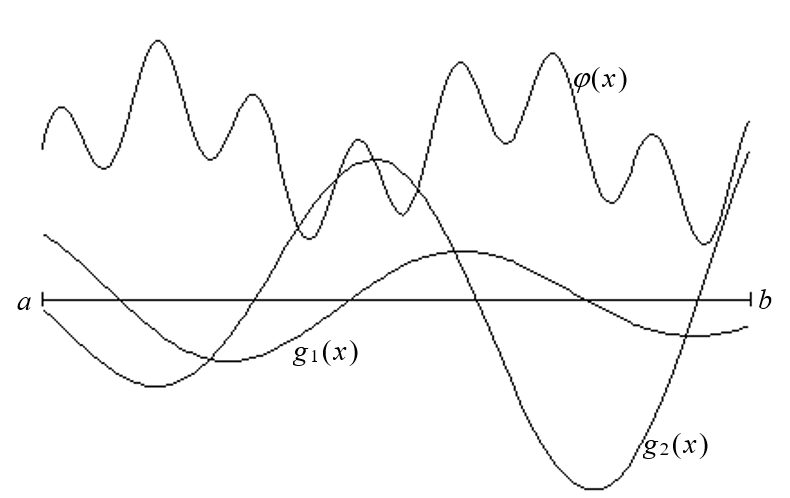
\includegraphics[width=0.8\textwidth]{figures/4_1.png}
  \caption{One-dimensional global optimization problem}
\end{figure}
}

\section{Partial computability and index scheme of the account of constraints}
Problem \eqref{eq4:problem} can be considered in the statement when each function $g_j,1\le j\le m+1$ is defined and computable only in the corresponding subdomains $Q_j\subset [a,b]$ where
\begin{equation}
  \label{eq4:q}
  Q_1=[a,b],Q_(j+1)=\{x\in Q_j:g_j(x)\le 0\},1\le j\le m.
\end{equation}

For example, in the optimal design problems some characteristics of the technical systems may appear to be undefined if the conditions of the system functioning represented by a part of the constraints of problem \eqref{eq4:problem} are not fulfilled.

Taking into account conditions \eqref{eq4:q}, initial problem \eqref{eq4:problem} can be represented in the form
\begin{equation}
  \label{eq4:problem2}
  \varphi(x^*)=\min\{g_{m+1}(x):x\in Q_{m+1}\}.
\end{equation}

For the purposes of further treatment, let us introduce a classification of the points $x$ in the search domain $[a,b]$ using an index $\nu=\nu(x)$ where $\nu-1$ is the number of constraints, which are fulfilled in this point. Formally, the index $\nu$ is defined by the conditions
\begin{equation}
  \label{eq4:condition}
  g_j(x)\le 0,1\le j \le \nu-1,g_\nu(x)>0,
\end{equation}
(the last inequality is inessential  if $\nu=m+1$) and it satisfies the inequalities
\begin{displaymath}
  1\le\nu=\nu(x)\le m+1.
\end{displaymath}
The problem of example \ref{ex4:problem} assuming a partial computability of the functions is presented in Fig. \ref{fig:4_2}. The arcs of the restrictions $g_1(x),\:g_2(x)$, and of the objective function $\varphi(x)$ defined in the corresponding subdomains $Q_j$ from \eqref{eq4:q} are shown. The point $x^1$ with the index $\nu(x^1)=1$, the point $x^2$ with the index $\nu(x^2)=2$, and the point $x^3$ with the index $\nu(x^3)=3$ are shown also.

\begin{figure}[h]
  \label{fig:4_2}
  \centering
  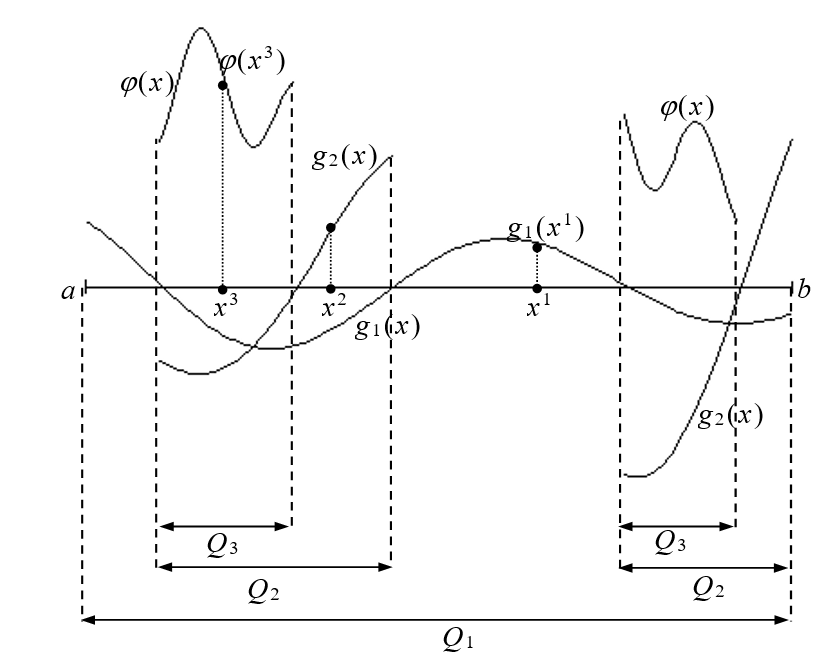
\includegraphics[width=0.8\textwidth]{figures/4_2.png}
  \caption{A problem with partially computable functions}
\end{figure}

This classification generates the function
\begin{equation}
  \label{eq4:fx}
  f(x)=g_\nu(x),\nu=\nu(x),
\end{equation}
defined and computable everywhere in $[a,b]$. Its value at a point $x$ is either the value of the left part of the constraint violated at this point (the case $\nu\le m$)  or the value of the objective function (the case $\nu=m+1$). Therefore, the determination of the value of $f(x),\:x\in[a,b]$  is reduced to a successive computations of the values of $g_j(x), 1\le j\le \nu=\nu(x)$, i.e., the next value $g_{j+1}(x)$ is calculated in the case when $g_j(x)\le 0$ only. The computational process finishes either as a result of the fulfillment of the inequality $g_j(x)>0$ or as a result of achievement of the value $\nu(x)=m+1$.

The described procedure called a \emph{trial} at the point $x$ forms the index $\nu$ of this point automatically. The pair of values
\begin{equation}
  \label{eq4:trial}
  z=f(x)=g_\nu(x),\nu=\nu(x)
\end{equation}
generated by the trial at the point $x\in[a,b]$ is called the \emph{trial result}.

The graph of the function $f(x)$ from \eqref{eq4:fx}, which consists of the arcs of the constraints $g_1(x),\:g_2(x)$, and of the objective function $\varphi(x)$ taken from Example \ref{ex4:problem} is shown in Fig. \ref{fig:4_3}.

\begin{figure}[h]
  \label{fig:4_3}
  \centering
  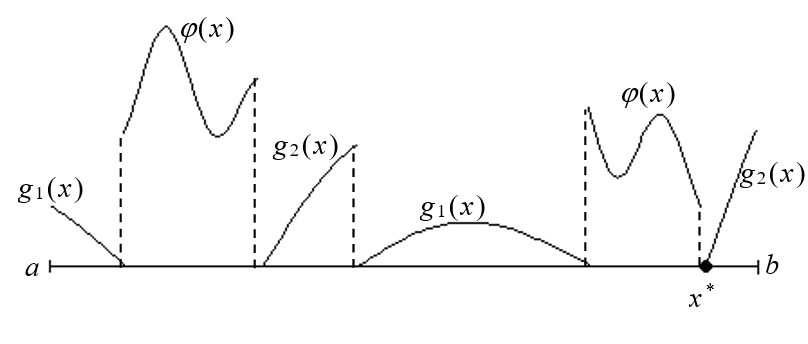
\includegraphics[width=0.8\textwidth]{figures/4_3.png}
  \caption{An ''index'' function}
\end{figure}

Since in the general case the problem \eqref{eq4:problem2} may have no solution (i.e., the feasible subdomain $Q_{m+1}$ might appear to be empty because of the incompatibility of the constrains) an auxiliary problem always having a solution is associated with it. Since conditions \eqref{eq4:condition} are equivalent to the conditions
\begin{displaymath}
  x\in Q_\nu,x\not\in Q_{\nu+1},
\end{displaymath}
this auxiliary problem can be written in the form
\begin{equation}
  \label{eq4:problem3}
  g_M^*=g_M(x_M^*)=\min\{g_M(x):x\in Q_M\},
\end{equation}
where $M$ is the greatest possible value of the index i. e.
\begin{equation}
  1\le M=\max\{\nu(x):x\in[a,b]\}\le m+1
\end{equation}
Since the set $Q_M$ is always nonempty, problem \eqref{eq4:problem3} always has a solution. When $M=m+1$ the solution $x^*=x^*_m+1$  is also the solution of the initial problem \eqref{eq4:problem}. When $M<m+1$ the inequality $g_M^*<0$ fulfilled necessarily can be used as an indicator of the incompatibility of the constraints.

The main idea of the index approach is to reduce the constrained problem \eqref{eq4:problem3} to a unconstrained one
\begin{displaymath}
  \psi(x^*)=\min\{\psi(x):x\in[a,b]\},
\end{displaymath}
where
\begin{equation}
  \psi(x)=
  \begin{cases}
    g_\nu(x)/L_\nu, & \nu < M, \\
    (g_M-g_M^*), & \nu=M.
  \end{cases}
\end{equation}

As a result, the arcs of $\psi(x)$ will be Lipschitzian with the constant $L=1$ in each subdomain $Q_\nu,1\le\nu\le M$. A graph of the function $\psi(x)$ for the example (\ref{ex4:problem}) is presented in Fig. \ref{fig:4_4}. This new function will have discontinuities of the first type at the boundary points of the subdomains $Q_\nu$ from \eqref{eq4:q}. Nevertheless, one can estimate the global minimizer $x^*_M$ using the results of $k$ trials for \eqref{eq4:trial} at the points $x_1,\dots, x_k$ in $[a,b]$ (see \cite{3}).

Indeed, as follows from Lipschitz condition
\begin{equation}
  \label{eq4:lip_opt_est}
  x^*_M\in\{x\in[a,b]:|x-x^i|\ge\psi(x^i),1\le i\le k\}.
\end{equation}

For example, a case for $k=4$ is presented in Fig. \ref{fig:4_4}. The union of the segments highlighted with a bold line in Fig. \ref{fig:4_4} is a complement of the set from the right hand side of \eqref{eq4:lip_opt_est} and does not include the optimum point.
\begin{figure}[h]
  \label{fig:4_4}
  \centering
  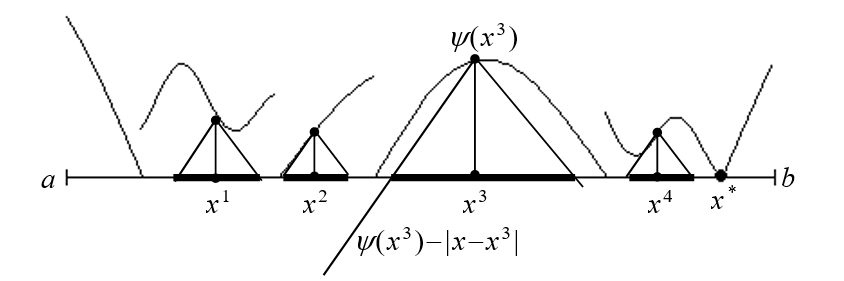
\includegraphics[width=0.8\textwidth]{figures/4_4.png}
  \caption{An estimate of the optimum point}
\end{figure}

Note that the greatest index $M$, the values of Lipschitz constants $L_\nu, 1\le \nu\le M$, and the value of $g_M^*$ are the unknowns. However, these problems can be overcome by means of using instead of them the adaptive estimates of these values obtained in the course of solving the problem on the base of trial results.

Having introduced all necessary concepts, let us turn to the description of the index algorithm.

\section{The index global search algorithm}
The first trial is executed at an arbitrary internal point $x_1\in(a,b)$. The selection of any subsequent trial point $x^{k+1},k\ge 1$ is determined by the following rules.

\emph{Rule 1.} Renumber the points $x^1,...,x^k$ of the preceding trials by the lower indices in ascending order of coordinate values, i.e.
\begin{equation}
  \label{eq4:search_data}
  0=x_0<x_1<\dots <x_k<x_{k+1}=1,
\end{equation}
and juxtapose to them the values $z_i=g_\nu(y(x_i)), \; \nu=\nu(x_i), \; 1
\leq i \leq k$, from \eqref{eq4:fx}; the points $x_0=0$ and
$x_{k+1}=1$ are introduced additionally for the convenience  of further notation (the values $z_0$ and $z_{k+1}$ are not defined).

\emph{Rule 2.} Classify the indices $i, \; 1 \leq i \leq k$, of the trial points from set \eqref{eq4:search_data} according to the number of the problem constraints fulfilled at these points, by constructing the sets
\begin{equation}
  I_\nu =\left\{i:1 \leq i \leq k, \; \nu=\nu(x_i) \right\}, \; 1 \leq \nu \leq m+1,
\end{equation}

containing the numbers of all the points $x_i, \; 1 \leq i \leq k$, with
the same values of $\nu$. The end points $x_0=0$ and $x_{k+1}=1$ are
interpreted as the ones having indices equal to zero. An additional set,
$I_0=\left\{0,k+1\right\}$, corresponds to them.

\emph{Rule 3.} Determine the maximum value of the index:
\begin{equation}
  M=\max\left\{\nu(x_i), \; 1 \leq i \leq k \right \}.
\end{equation}

\emph{Rule 4.} Compute the current lower estimates,
\begin{equation}
  \label{eq4:lip_est}
  \mu = \max\left\{ \frac{\left|z_i-z_j\right|}{ x_i - x_j }, \; i,j \in I_\nu, \; i>j \right\},
\end{equation}
for the unknown Lipschitz constants $L_\nu$ of the functions $g_\nu(y),1
\leq \nu \leq m+1$. If a set $I_\nu$ contains less than two elements, or
if $\mu_\nu$ is equal to zero, then assume $\mu_\nu=1$. As follows from \eqref{eq4:lip_est}, the estimates $\mu_\nu$ are non-decreasing starting from the moment when \eqref{eq4:lip_est} generates a positive value $\mu_\nu$.

\emph{Rule 5.} For all nonempty sets $I_\nu, \; 1 \leq \nu \leq m+1$, compute the estimates
\begin{equation}
  \label{eq4:z_const}
  z_\nu^\ast = \left\{
  \begin{array}{lr}
    0, & \nu < M,\\
    \min\{ g_\nu(y(x_i): i\in I_\nu \}, & \nu = M.
  \end{array}
  \right.
\end{equation}

\emph{Rule 6.} For each interval ($x_{i-1},x_i), \; 1 \leq i \leq k+1,$ compute the \textit{characteristics} $R(i)$:
\begin{gather}
  \label{eq4:characteristic}
  R(i)=2\Delta_i-4\frac{z_i-z_\nu^\ast}{r_\nu \mu_\nu}, \; \nu=\nu(x_i)>\nu(x_{i-1}), \nonumber \\
  R(i)=\Delta_i+\frac{(z_i-z_{i-1})^2}{r_\nu^2 \mu_\nu^2\Delta_i}-2\frac{z_i+z_{i-1}-2z_\nu^\ast}{r_\nu \mu_\nu}, \;  \nu=\nu(x_i)=\nu(x_{i-1}),\\
  R(i)=2\Delta_i-4\frac{z_{i-1}-z_\nu^\ast}{r_\nu \mu_\nu}, \; \nu=\nu(x_{i-1})>\nu(x_i), \nonumber \\
  \Delta_i=x_i - x_{i-1} \nonumber
\end{gather}
The values $r_\nu>1, 1\le\nu\le m+1$ are the parameters of the algorithm. An appropriate choice of the values $r_\nu$ allows using the products $r_\nu\mu_\nu$ as the estimates of Lipschitz constants $L_\nu, 1\le\nu\le m+1$.

\emph{Rule 7.} Find the interval $(x_{t-1},x_t)$ with the maximum characteristic
\begin{equation}
\label{eq4:MaxR}
R(t)=\max{\left\{R(i): 1 \leq i \leq k+1\right\}}.
\end{equation}

\emph{Rule 8.} Make the next trial at the midpoint of the interval
$(x_{t-1},x_t)$ if the indices of the points $x_{t-1}$ and $x_t$  are not the same, i.e.
\[
x^{k+1} = \frac{x_t + x_{t-1}}{2}, \; \nu(x_{t-1}) \neq \nu(x_t).
\]
Otherwise, make the trial at the point
\begin{equation}
\label{eq4:next_point}
x^{k+1} = \frac{x_t+x_{t-1}}{2} - \frac{z_t-z_{t-1}}{2r_\nu\mu_\nu},\; \nu=\nu(x_{t-1})=\nu(x_t).
\end{equation}

The described rules can be supplemented with the termination condition, finalizing the iterations of the method if
\begin{equation}
\label{eq4:stop_cond}
  x_t - x_{t-1}\le\epsilon
\end{equation}
where $t$ from \eqref{eq4:MaxR} and $\epsilon>0$ is the predefined accuracy of the optimization.

Let us formulate the conditions of convergence for the algorithm in the form of the following theorem.
\begin{theorem}
Let the considered index algorithm be applied to the solving of problem \eqref{eq4:problem} and the following conditions be satisfied:
\begin{enumerate}
  \item each function $gj, 1\le j\le m+1$ satisfies Lipschitz condition with the constant $L_j$ in the interval $[a,b]$, i.e.,
  \[
  |g_j(x_1)-g_j(x_2)|\le L_j|x_1-x_2|,1\le j\le m+1,x_1,x_2 \in[a,b]
  \]
  \item the following inequalities hold for the quantities $\mu_\nu$ from \eqref{eq4:lip_est} starting from some step
  \[
  r_\nu\mu_\nu > 2L_\nu,1\le\nu\\le m+1.
  \]
\end{enumerate}

Then the set of the limit points of the sequence $\{x_k\}$ generated by the index algorithm coincides with the set of solutions of problem \eqref{eq4:problem} with $\epsilon=0$ and termination criterion \eqref{eq4:stop_cond}. In addition, the index of each limit point equals to $M$ and the convergence to any limit point $\overline{x}$  is bilateral if $\overline{x}\not=a$ and $\overline{x}\not=b$.
\end{theorem}

This theorem is given without a proof, which can be found, for example, in \cite{}[1, 2]. Various modifications of this algorithm and the corresponding theory of convergence are given in \cite{}[5–10].

\textbf{The results of the experiment.} Let us consider a problem from Example (\ref{ex4:problem}) as an illustration. Under assumption of partial computability the arcs of the problem functions corresponding to the domains $Q_j, 1\le j\le 3$, from \eqref{eq4:q} are presented in Fig. \ref{fig:4_6}.

Three methods have been used for solving this example:
\begin{enumerate}

  \item Scanning a uniform grid with the precision (distance between adjacent nodes) $\epsilon=10^{-5}$.
  \item Penalty function method, i.e., the minimization of the function
  \[
  p(x)=\varphi(x)+(\max\{g_1(x),0\})^2+(\max\{g_2(x),0\})^2
  \]
  using Algorithm of Global Search. The coordinates of the trial points executed by AGS in the process of problem solving are marked by the vertical strokes in Fig. \ref{fig:4_5}. The coordinates of the trials executed in the close points are marked by a dark rectangle.
  \item Index algorithm with the parameters $r_\nu=2, 1\le \nu \le 3$, and $\epsilon =10^{- 5}$. The trial point coordinates executed by the algorithm in the course of problem solving are marked by three rows of the vertical strokes in Fig. \ref{fig:4_6}. The strokes in the upper row correspond to the points with the index $\nu=1$, the ones of the second row --- to the points, the indices of which are equal to 2; and the points marked by the strokes in the bottom row are the feasible ones. The trial coordinates performed in the close points are marked by a dark rectangle.
\end{enumerate}

\begin{figure}[h]
  \label{fig:4_5}
  \centering
  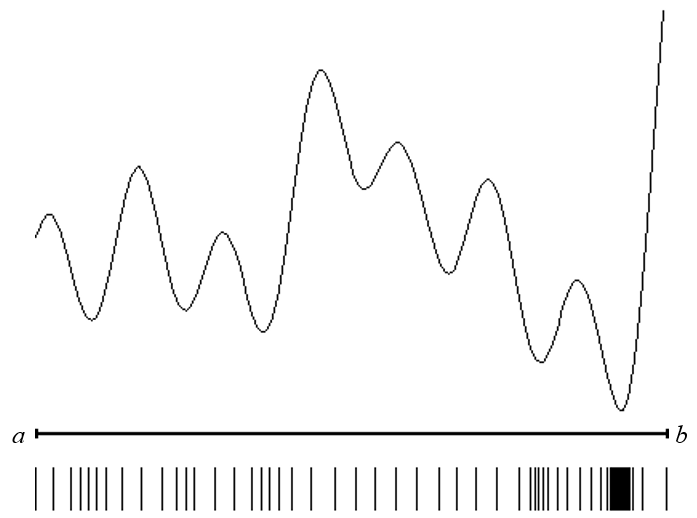
\includegraphics[width=0.8\textwidth]{figures/4_5.png}
  \caption{Minimization by means of Penalty Function Method}
\end{figure}

It is worth noting, that in the applied problems the estimates of the constraints as well as of the objective functions require considerable computation resources very often. The results presented in Table \ref{tab4:exp_results} confirm the effectiveness of the index scheme of the account of
constraints.

\begin{table}
  \caption{}
\begin{center}
  \label{tab4:exp_results}
  \begin{tabular}{| l | c | c | c| }
    \hline
    & $k_1$ & $k_2$ & $k_3$ \\ \hline
    Scanning a uniform grid & 160000 & 90280 & 56476 \\ \hline
    Penalty Function Method &  375 & 375 & 375 \\ \hline
    Index method & 63 & 49 & 35 \\ \hline
  \end{tabular}
\end{center}
\end{table}

Here $k_i$ is the number of computations of the $i$ problem function, i.e., of the function $g_i(x )$.
\begin{figure}[h]
  \label{fig:4_6}
  \centering
  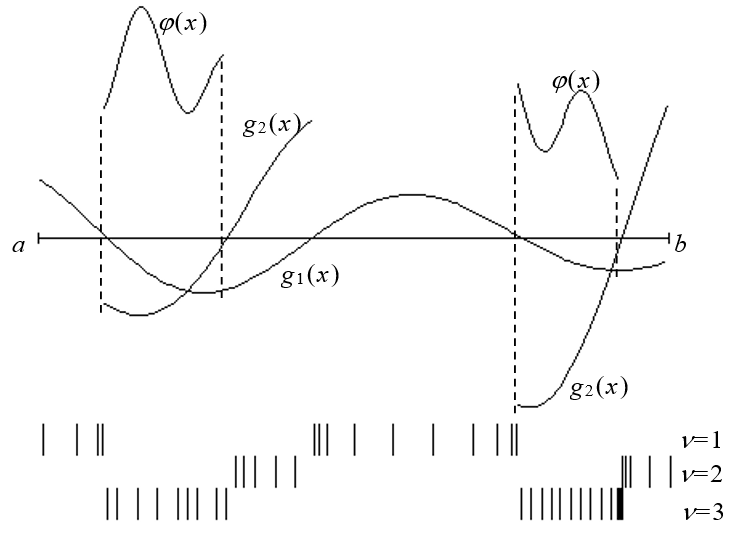
\includegraphics[width=0.8\textwidth]{figures/4_6.png}
  \caption{The minimization of an ''index'' function}
\end{figure}

\section{Index algorithm taking into account the existence of $\epsilon$-reserved solutions}
Let us return to the consideration of a one-dimensional problem of the kind \eqref{eq4:problem}
\begin{displaymath}
  \varphi(x^*)=\min\{\varphi(x):x\in [a,b], g_j(x)\le 0,1\le j\le m\}
\end{displaymath}
In the case when the objective function and the left-side parts of the constraints are partially computable, it is necessary to use the form \eqref{eq4:problem2}.
\example
{
Let us consider problem \eqref{eq4:problem} with $x\in[0,6,2,2]$, $m=3$ as an illustration:
\begin{gather*}
\varphi(x)=\cos(18x-3)\sin(10x-7)+1, \\
g_1(x)=\exp(-x/2)\sin(6x-1.5) \\
g_2(x)=\sin(4x-2.2)+\cos(6x-2.9) \\
g_3(x)=|x|\sin(2\pi x - 0.5).
\end{gather*}
}
\begin{figure}[h]
  \label{fig:4_7}
  \centering
  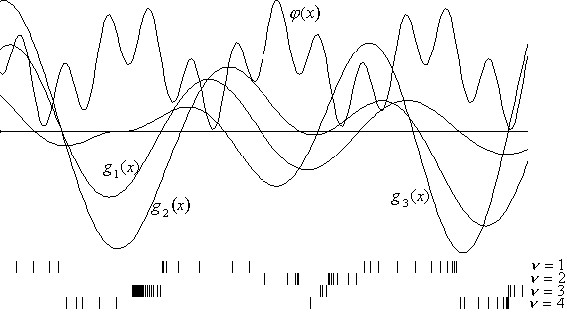
\includegraphics[width=0.8\textwidth]{figures/4_7.jpg}
  \caption{The solution of a problem by Index Method}
\end{figure}
The functions $g_j , 1\le j\le 4$, are pictured in Fig. \ref{fig:4_7}. Assuming a partial calculability, the arcs of
the functions corresponding to the domains $Q_j ,1\le j\le 4$, from \eqref{eq4:q} are presented in Fig. \ref{fig:4_8}.

\begin{figure}[h]
  \label{fig:4_8}
  \centering
  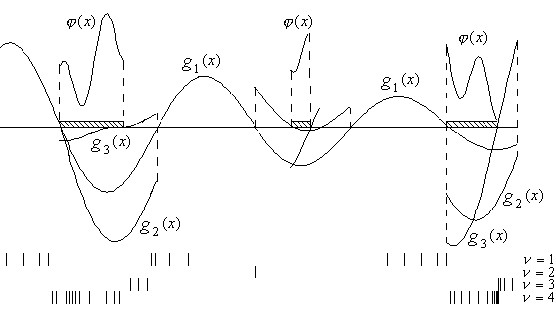
\includegraphics[width=0.8\textwidth]{figures/4_8.jpg}
  \caption{The problem solving by Index Method with the $\epsilon$-reservs}
\end{figure}

Index algorithm described in Sec. 3.3 was used to solve this example with $x_1=(a+b)/2$, $r=2$, and $\varepsilon=10^{-5}$. The coordinates of 102 trial points executed by the algorithm in the process of problem solving are marked by four rows of the vertical strokes in Fig. \ref{fig:4_7}. The strokes of the upper row correspond to the points with the index $\nu=1$, the ones of the second and the third rows --- to the points, the indices of which are equal to 2 and 3, respectively; and the points
marked by the strokes of the bottom row are feasible.

The coordinates of the trials executed in the close points are marked by a dark rectangle. The values of the functions $g_1 , g_2 , g_3$ , and $\varphi=g_4$ have been computed $k_1=102$, $k_2=80, k_3=64,$ and $k_4=26$ times, respectively. As one can see in Fig. \ref{fig:4_7}, the trial points concentration takes place not only in the vicinity of the point of the global optimum $x^*=2,07957$, but also in the vicinities of the inadmissible boundary points of the domains $Q_j$ from \eqref{eq4:q}. This effect can be reduced by the substitution of estimates \eqref{eq4:z_const} by the estimates
\begin{equation}
  z_\nu^\ast = \left\{
  \begin{array}{lr}
    -\epsilon_\nu, & \nu < M,\\
    \min\{ g_\nu(y(x_i): i\in I_\nu \}, & \nu = M.
  \end{array}
  \right.
\end{equation}
where $\epsilon_R=(\epsilon_1 ,\dots, \epsilon_m)$ is a predefined vector with positive components. Thus, $z^*=0$ if there exist the points $x_i,1\le i\le k$ from series \eqref{eq4:search_data} with the index greater than $\nu$. As a consequence of this substitution the values of the characteristics $R(i)$ from \eqref{eq4:characteristic} will become lower (because of the subtraction of $\epsilon_\nu$) if
\begin{equation}
  \nu=\max\{\nu(x_{i-1},\nu(x_i)\}<\max\{\nu(x_j):1\le j\le k\}\le V
\end{equation}
that makes executing the trials in the corresponding intervals  ($x_{i-1}$ , $x_i$ ) less probable. In all other aspects, the algorithm remains the same.

This \emph{prima facie} mechanical trick has a well-established theoretical basis considered below.

\begin{definition}
  The point $x_\epsilon$ is called an $\epsilon$-reserved solution of problem \eqref{eq4:problem} if the condition
  \begin{equation}
    \label{eq4:eps_res_problem}
    \varphi(x_\epsilon)=\min\{\varphi(x):x\in [a,b], g_j(x)\le -\epsilon_j,1\le j\le m\}
  \end{equation}
  meets where $\epsilon_1, \dots,\epsilon_m$ are the positive values of reserve for each constraint. Let us introduce into consideration also the set
  \begin{equation}
    \label{eq4:x_epsilon}
    X_\epsilon = \{x\in[a,b]:g_j(x)\le 0, 1\le j\le m, \varphi(x)\le\varphi(x_\epsilon)\}
  \end{equation}
  of all feasible solutions of the problem, which are no worse with respect to the objective function value than the $\epsilon$-reserved solution.
\end{definition}

The existence of the $\epsilon$-reserved solution of problem \eqref{eq4:problem} can be interpreted as some analogue of the conditions of regularity in the classical nonlinear programming problems. The applied role of this condition should be noted also. Even if the exact solution $x^*$ is known, its practical implementation is possible as some approximation to $x^*$ only. Therefore, the existence of the feasible points from $Q$ close to $x^*$ (with respect to the coordinates and to the objective
function values) is important. The existence of the $\epsilon$-reserved solution guarantees the availability of such points. Moreover, the domain $X_\epsilon$ may play a role of the set of suitable approximations.

The index algorithm with the $\epsilon$-reserves has been applied to the considered example with $\epsilon_i=0.2, 1\le i\le 3$. The search trial coordinates are marked by the vertical strokes in Fig. \ref{fig:4_8}. The solution has required 52 trials only and provided the same precision of the problem solution as in
the case when the vector $\epsilon_R$ equals to zero. Moreover, the values of the functions $g_1$ , $g_2$ , $g 3$ , and $\varphi=g_4$ have been calculated $k_1 =52$, $k_2 =39$, $k_3 =38$, and $k_4 =25$ times, respectively.

The conditions of convergence for the algorithm are presented in the following theorem (given without proof, see \cite{}).

\begin{theorem}
  Assume problem \eqref{eq4:problem} to have a solution $x^*$ and the following conditions to be satisfied:
  \begin{enumerate}
    \item each domain $Q_j ,1\le j\le m+1$ from \eqref{eq4:q} is a union of a finite number of positive length segments;
    \item each function $g_j ,1\le j\le m+1$ allows Lipschitz extension $G_j (x)$ with the constant $L_j$ over the whole interval $[a,b]$, i.e.,
    \begin{equation}
      g_j(x)=G_j(x),x\in Q_j,1\le j\le m+1;
    \end{equation}
    \item the components $\epsilon_\nu$ of the reserve vector $\epsilon_R$ corresponding to the constraints being active at the absolute minimum point $x^*$ (i.e., the constraints, for which $g_\nu(x^*)=0$) satisfy the inequalities
    \begin{equation}
      \label{eq4:reserves}
      0<2\epsilon_\nu<L_\nu(\beta-\alpha)
    \end{equation}
    where $\beta-\alpha$ is the length of the interval $[\alpha,\beta]\subset Q_{m + 1}$ containing the point $x^*$;
    \item the components $\epsilon_\nu$ of the reserve vector $\epsilon_R$ corresponding to the constraints which are not active at the absolute minimum point $x^*$ (i.e., $g_\nu(x^* )<0)$ satisfy either inequalities \eqref{eq4:reserves} or the inequalities
    \begin{equation}
      0< \epsilon_\nu <|g_\nu (x^* )|;
    \end{equation}
  \end{enumerate}

  Then:
  \begin{enumerate}
    \item the point $x^*$ is the limit point of the trial sequence $\{x_k \}$ generated by index algorithm for problem \eqref{eq4:problem} at $\epsilon =0$ in the termination condition \eqref{eq4:stop_cond};
    \item any limit point $\overline x$ of the sequence ${x_k }$ is a solution of the problem \eqref{eq4:problem};
    \item the convergence to the limit point $x$ is a bilateral one if $x\not=a$ and $x\not=b$.
    If the conditions \eqref{eq4:reserves} and (4.27) are not satisfied for given vector of reserves $\epsilon_R$ but the
    problem $\eqref{eq4:problem}$ has an $\epsilon$-reserved solution $x_\epsilon$ defined by \eqref{eq4:eps_res_problem}, then:

    \item for any limit point $x$ of the sequence ${x_k}$ it is true that
    \begin{displaymath}
      \varphi(\overline x)=\inf\{\varphi(x^k):g_j(x^k)\le 0,\: 1\le j\le m,\: k=1,2,\dots\}\le\varphi(x_\epsilon);
    \end{displaymath}
    \item any limit point $\overline x$ is a boundary point of the set $X_\epsilon$ from \eqref{eq4:x_epsilon} if the function $\varphi(x)$ has no more than one point of local maximum in each of the isolated intervals making up the set $X_\epsilon$;
    \item the above statement on the bilateral character of the convergence remains in force.
  \end{enumerate}
\end{theorem}

As it has been demonstrated by the experiment with solving the example described above, the increase of the reserve values may result in an essential decrease of the trial concentration in the boundary points of non-feasible domains. The theoretical properties of the trial sequences generated by the index algorithm are determined by the following statement (see the proof in \cite{}[4] also).
\begin{theorem}
  Assume the convergence conditions for the index algorithm to be satisfied and the inequalities
  \begin{displaymath}
    g_\nu(x)\ge\delta_\nu,x\in[\alpha,\beta],\delta_\nu\ge 0
  \end{displaymath}
  to be satisfied in a subinterval $[\alpha,\beta]\subset Q_\nu \: 1\le\nu\le m$, the length of which meets the condition
  \begin{displaymath}
    \beta-\alpha>\frac{2(r_\nu-1)(\delta_\nu+\epsilon_\nu)}{r^2_\nu L_\nu}.
  \end{displaymath}

  Then for the density $P_{\alpha\beta}$ of the points from the sequence $\{x_k\}$ generated by the index algorithm while solving the problem \eqref{eq4:problem} there is the estimate
  \begin{displaymath}
    P_{\alpha\beta}<\frac{r^2_\nu L_\nu}{(r_\nu-1)(\delta_\nu+\epsilon_\nu)}.
  \end{displaymath}
\end{theorem}

\textbf{Selection of components of the vector of reserves.} A problem of the choice of concrete component values in the vector of reserves $\epsilon_R$ arises when applying the considered algorithm.
The convergence theorem can help in solving this problem. Condition \eqref{eq4:reserves} can be considered as a recommendation for the selection of the reserve values, for which the property of
convergence to the solution of problem \eqref{ex4:problem} remains. However, in the general case the values of Lipschitz constants are not given \emph{a priori}, and the length of the interval $[\alpha,\beta]$ from $Q_{m + 1}$, including the sought solution $x^*$ is not kwon also. These difficulties are possible to avoid by
substitution of the unknown coefficients $L_j,\: 1\le j\le m$, by their adaptive underestimates $\mu_\nu$ from (4.15) and by assumption that $\beta-\alpha>\delta=\epsilon q$ where $\epsilon >0$ (accuracy) is a parameter defined in the termination condition and the factor $q>1$ can be interpreted as an a priori estimate of how many times the length of the interval $[\alpha,\beta]$ is greater than given accuracy $\epsilon$. As a result, one can take
the reserve estimates in the form (adaptive reserves)
\begin{displaymath}
  \epsilon_\nu=\mu_\nu\delta,\: 1\le\nu\le m.
\end{displaymath}

\textbf{The results of the experiment.} In order to demonstrate the efficiency of the adaptive reserves, a series of problems with the multiextremal constraints has been solved.

Let us consider a generator $G$ generating the problems with $m$ constraints on the base of a random mechanism $F$ producing the functions $f(x),\: x \in [ a , b ]$. The rules determining the
functioning of this mechanism $G$ consist in the following.
\begin{enumerate}
  \item $m+1$ functions $f_j(x),\: 1\le j \le m+1,\: x\in[a,b]$, are generated independently by means of given mechanism $F$.
  \item The minimax value
  \begin{displaymath}
    \Delta=\min_{a\le x\le b}\max_{1\le j\le m}f_j(x),
  \end{displaymath}
  is calculated and the left-hand parts of the constraints
  \begin{equation}
    \label{eq4:generated_g}
    g_j(x)=f_j(x)-\Delta\delta,\: 1\le i\le m,
  \end{equation}
  which a nonempty feasible domain $Q$ corresponds to at $\delta>0$ are introduced. Increasing the value of the parameter $\delta$ allows to expand the feasible domain.
  \item Function \eqref{eq4:generated_g} and the objective function $\varphi(x)=f_{m+1}( x )$ form a problem of the kind \eqref{eq4:problem} obviously having a solution.
\end{enumerate}

n the cases, when it is necessary to denote the parameters $m$ and $\delta$ used by the generator during its functioning, let us use the notation $G ( m , \delta )$. In the experiments, the results of whichare presented below two generators were employed. One of these (let us denote it as $G_{SH} ( 5 , 1 ) )$ was based on the function
\begin{displaymath}
  \varphi(x)=-\sum_{j=1}^{10}\frac{1}{(K_j(x-A_j)^2+C_j)}x\in[0,10].
\end{displaymath}
$1\le K_j\le 3,\: 0\le A_j,\: C_j\le 10 $, where the parameters $K_j,\: A_j,\: C_j ,\: 1 \le j \le 10$ are the independent random variables distributed uniformly over the intervals specified above. The second generator hereinafter denoted as $G_{HL} ( 5 , 1 ) )$ was based on the function
\begin{equation}
  \varphi(x)=\sum_{j=1}^{14}(A_j\sin(2j\pi x) + B_j\cos(2j\pi x)),\: x\in[0,1]
\end{equation}
where the values of the parameters $A_j,\: B_j,\: 1 \le j \le 14$, are distributed independently and uniformly over the interval $[-1 ,1 ]$. Both generators were applied to the generation of 100 own
problems of the kind \eqref{eq4:problem}.

The problems were solved by the initial index algorithm as well as by the algorithm with $\epsilon$-reservation. The parameters $r_\nu ,\: 1 \le \nu \le 6$, from (4.17) were chosen as
\begin{displaymath}
  r_\nu = \left\{
  \begin{array}{lr}
    \gamma, & k_\nu < 20\\
    2, & k_\nu \ge 20
  \end{array}
  \right.,
\end{displaymath}
where $k_\nu$ is the number of the computed values of the function $g_\nu$ (i.e., the cardinality of the set $I_\nu$). In the test set generated by generator $G_{SH}$ the values $\gamma=20,\: \epsilon = 0.001$ and the reserves $\delta_\nu=0.02,\: 1 \le \nu \le 5$, were used in the experiments. For the problems from the second test set
(generated by $G_{HL}$ ) the values $\gamma = 10, \epsilon=0.0001$ and the parameters $\delta_\nu=0.001,\: 1 \le \nu\le 5$, were used.

\begin{figure}[h]
  \label{fig:4_9}
  \centering
  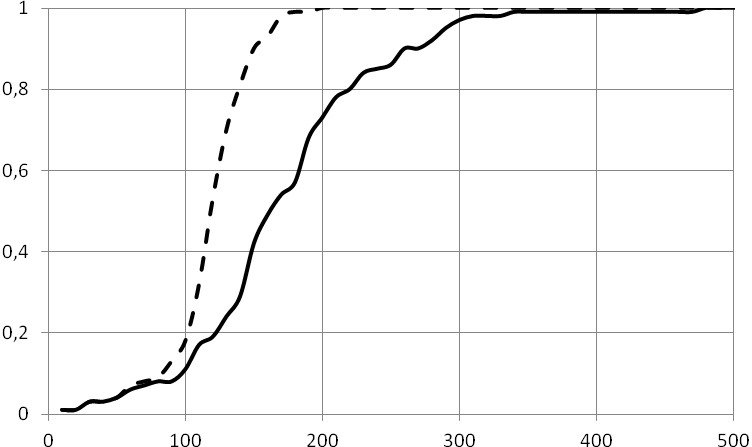
\includegraphics[width=0.8\textwidth]{figures/4_9.png}
  \caption{The operation characteristics in class $G_{SH}$}
\end{figure}

\begin{figure}[h]
  \label{fig:4_10}
  \centering
  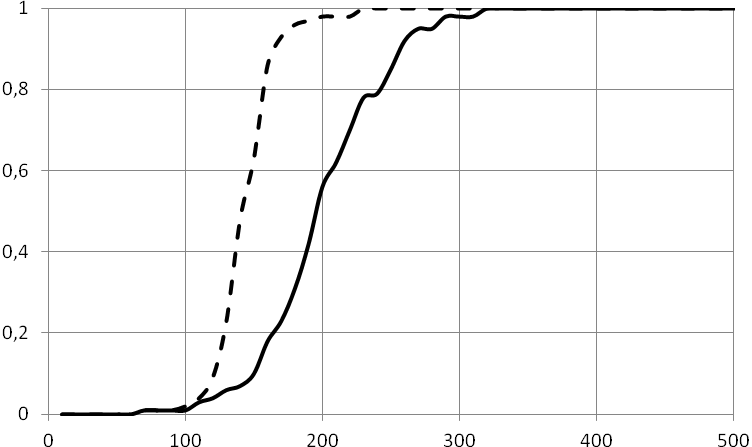
\includegraphics[width=0.8\textwidth]{figures/4_10.png}
  \caption{The operation characteristics in class $G_{HL}$}
\end{figure}

The operational characteristics for both method obtained for the test problem sets generated by $G_{SH}$ and $G_{HL}$ are presented in Figures 4.9 and 4.10, respectively. The lower (solid) curves refer to the initial index algorithm while the upper (dashed) ones correspond to the index algorithm with the adaptive reserves. Such arrangement of the curves demonstrates the algorithm with the
adaptive reserves to provide much faster obtaining the estimates falling into given vicinity of the solution than the initial index algorithm. The average numbers of iterations for the method
without the reserves and for the method with the adaptive reserves were equal to 171 and 117 for the problems $G_{SH}$ and 199 and 142 for the ones $G_{HL}$ , respectively.

\section{Index method with adaptive order of checking for constraints}
According to the rules of the index method considered in the preceding subsections, every trial includes the successive check of the fulfillment of the problem constraints in the corresponding point of the search domain. The finding of the first violated constraint terminates the trial and initiates the transition to the next iteration. If a numeration of the constraints in the increasing order by the computational costs of their checking is introduced (i.e., if the simpler constraints are checked first) one can reduce essentially the overall computational costs in the course of optimization. The above is important for the problems, in which the estimating of the function value requires a considerable computational resources connected with a necessity of the numerical modelling of the behavior of the systems described by these functions (as it takes place, for example, in numerous problems of the optimal design).

Obviously, the computational expenditures of the trial execution depend on the order of the problem functions’ computation essentially. If the calculation time of any problem is independent on the iteration execution point, the less the number of the problem functions (constraints and objective function) calculated at a point x, the less the trial execution costs in this point.

For many applied problems, it is naturally to assume that a constraint violated at a point in the search domain, will be violated in some neighborhood of this point as well. In this case, it might be useful to begin the next trials in the points of this neighborhood with checking the fulfillment of this particular constraint. In the scope of the above, it seems reasonable to design a global optimization algorithm allowing the modification of the constraint  check order taking into account the information obtained during the search. The check order design will be oriented onto the constraint violated at an iteration point to be found as early as possible.

Let us now turn to the generalization of the scheme described in sections 3.3 and 3.4 onto the case when the constraint check order is not a fixed one. For further consideration, the initial algorithm described above will be referred to as \emph{Fixed Check Order Method} (FCOM).

The algorithm proposed below allows the modification of the constraint order check during solving the problem \eqref{eq4:problem}. These modifications are firstly directed onto analyzing during the current iteration the constraint violated at the end of the interval including the current iteration point. As it has been already mentioned above, such an approach might reduce the number of checks at the new trial point since the violation of this constraint in a vicinity of already found violation might be quite probable. Hence, the need in new rules for the juxtaposition of the indices to the points from \eqref{eq4:search_data} (remind, that these indices determine the use of expressions \eqref{eq4:characteristic} for the computation of the characteristics) as well as in a special order
of the constraint check at the current trial point arises. Note that the formation of such order is inessential for the intervals, the ends of which belong to a feasible domain $Q$ from \eqref{eq4:Q_union} since a necessity for checking all constraints is probable in such intervals.

Assume the constraint with the number $j,\: 1\le j\le m$, to fulfill at all points of the domain
\begin{equation}
  Q_j=\{x\in[a,b]:g_j(x)\le 0\},\: 1\le j\le m,
\end{equation}
which hereinafter will be called the feasible domain for this constraint. The feasible domain $Q$ of initial problem \eqref{eq4:problem} can be defined by the condition
\begin{equation}
  \label{eq4:Q_union}
  Q=Q_1\cap\dots\cap Q_m.
\end{equation}

\textbf{The constraints’ check order.} he numbering of the constraints and the objective function introduced in the statement of problem \eqref{eq4:problem} and defined by the sequence of integer numbers
\begin{equation}
  \label{eq4:basic_h}
  H=\{1,2,\dots,m,m+1\},
\end{equation}
will be considered as a base one.
Assume that every particular point $x$ from the search domain $[a,b]$ can have its own order of the problem constraints’ checking. The order of such checking corresponding to the point $x_i$ from (4.12) will be defines as some permutation $H(x_i )$ of the basic numbers from \eqref{eq4:basic_h}, i.e.,
\begin{equation}
  H(x_i)=\{j_{i1},\dots,j_{im},j_{i,m+1}\},\:0\le i\le k,
\end{equation}
where
\begin{equation}
  j_{i,m+1}=m+1,\:0\le i\le k.
\end{equation}

Since the constraints’ check order while the trial execution at the point $x$ i is determined by the corresponding tuple $H(x_i )$ from (4.33), the termination of the trial at this point after the computation of the values of l problem functions produces the value $z_i=g_\nu(x_i)$ where $\nu=j_{il}$. In this connection, let us use not the serial number $l$ of the last function calculated in this point, as it was accepted in (4.7) but the index of the last function in the basic numeration (4.32) as the
value of $\nu(x_i )$ for the point $x_i$ , i.e.,
\begin{equation}
  \nu(x_i)=j_{il}.
\end{equation}

\textbf{Algorithm.} The trial selection rules for Fixed Check Order Method (FCOM) already considered above give the base of the new algorithm scheme, which will be called \emph{Adaptive
Check Order Method} (ACOM). Since the alterable constraint check order excludes a possibility to use expression (4.13) to determine the sets $I\nu$, to construct them, an information array connecting each $x_i$ from (4.12) with the indices of all functions, which have been computed in this node is necessary. Hereinafter, the existence of such database is presumed. The rest modifications consist in the following.

\emph{Modification 1 (the fixation of the check order)}. Each point $x_i$ from \eqref{eq4:search_data} is assigned the corresponding checking order $H(x_i )$ from (4.33), and this order is included into the algorithm database.

\emph{Modification 2 (the determination of the trial points’ indices).} Each point $x_i$ from \eqref{eq4:search_data} is assigned the value $z_i=g_\nu(x_i)$ where according to (4.35), the index $\nu=\nu(x_i)$ is the basic index from (4.32) corresponding to the value of the last function estimated in this point. These indices are used in all computations based on expressions (4.13)– (4.17), (4.19).

The modifications in the method of using the indices are related to rules (4.17) of calculations of the characteristics $R(i)$ of the intervals $(x_{i-1},x_i),\: 1\le i\le k$, with noncoincident
indices of the boundary points only. Assume
\begin{equation}
  \nu(x_{i-1})=j_{i-1,p}=j_{i,q}\not=\nu(x_i)=j_{i-1,u}=j_{i,x},
\end{equation}
i.e., the problem function with the basic index $\nu(x_{i-1})$ has the index $p$ in the sequence $H(x_{i-1})$ corresponding to the point $x_{i-1}$ and the index $q$ in the sequence $H(x_i)$ corresponding to the point $x_i$. Analogously, the function with the basic index $\nu(x_i)$ corresponds to the index $u$ from the sequence $H(x_{i-1})$ and the index s from the sequence $H(x_i)$. Then, the introduced modification altering the sixth rule of FCOM consists in the following.

If for the indices $p,q, u$ and $s$ from (4.36) the conditions
\begin{equation}
  p<u,q<s,
\end{equation}
are fulfilled, in order to determine the characteristic $R(i)$ one should use the second expression from formulae (4.17) with $\nu=\nu(x_i)$ (note that in this case the value $g_\nu(x_{i-1})$ is undefined).

Otherwise, when the reverse to (4.37) conditions are fulfilled
\begin{equation}
  p>u,q>s,
\end{equation}
the characteristic $R(i)$ is defined by the third expression from (4.17) with $\nu=\nu(x_{i-1})$ (in this
case, the value $g_\nu(x_i ) is undefined)$. In the cases when conditions (4.37) and (4.38) are not fulfilled, the initial order of calculations prescribed by the sixth rule of the initial algorithm remains.

\emph{Modification 3 (the choice of the constraints’ check order in the current trial point).} Assume that the constraints’ check order corresponding to the first two trial points is defined by
the conditions
\begin{equation}
  H(a)=H(b)=H,
\end{equation}
where $H$ from (4.32). Let
\begin{displaymath}
  p=\nu(x_{t-1}),\: q=\nu(x_t)
\end{displaymath}
are the indices of the boundary points of the interval $(x_{t-1},x_t)$ including the current trial point $x^{k+1}$ (according to the eighth rule) determined according to (4.35). Let us introduce a notation $\{s,H\backslash s\}$ for the tuple obtained from $H$ by excluding the index $s$, shifting all indices $1,2,\dots,s-1$ to the right of one position, and the transfer of the index s excluded from $H$ into the first position, i.e.,
\begin{displaymath}
  \{s,H\backslash s\}=\{s,1,2,\dots,s-1,s+1,\dots,q-1,q+1,\dots,m+1\}.
\end{displaymath}
When $1\le p\le q\le m$, the superposition of the operations of the type described above produces the tuple of the kind
\begin{displaymath}
  \{p,\{q,H\backslash q\}\backslash p\}=\{p,q,1,\dots,p-1,p+1,\dots,q-1,q+1,\dots,m+1\}.
\end{displaymath}
Note that according to (4.34), the index $m+1$ always occupies the last position.

Now let us agree to determine the order $H(x^{k+1}),\: k\ge 1$ according to the following rules:
\begin{gather}
 H(x^{k+1})=H,\: p=q=m+1, \nonumber \\
 H(x^{k+1})=\{p,H\backslash p\}, (p=q<m+1)\cup(p<q=m+1), \nonumber \\
 H(x^{k+1})=\{q,H\backslash q\}, p=m+1>q\\
 H(x^{k+1})=\{p, \{q,H\backslash q\}\backslash p\}, p<q\le m \nonumber \\
 H(x^{k+1})=\{q, \{p,H\backslash p\}\backslash q\} m\ge p>q. \nonumber
\end{gather}

\textbf{Note.} While solving the problem \eqref{eq4:problem} rules (4.39) and (4.40) included into the scheme of ACOM assign the index values from (4.35) to all trial points unambiguously. Then, any feasible point $x$ always corresponds to the index $\nu(x)=m+1$. This value can be predicted before the trial execution in such point as well. However, if the point $x$ is not a feasible one and does not belong to the points, in which the trials have been executed already, the index value can be undefined in this point.

The convergence conditions for the algorithm are formulated in the following theorem.

\begin{theorem}
Assume problem \eqref{eq4:problem} to have a solution $x^*$ and the following conditions are fulfilled:
\begin{enumerate}
  \item each domain $Q_j ,1\le j\le m+1$ from (4.30) represents a union of a finite number of segments with a positive length;
  \item each function $g_j(x): 1\le j\le m+1$ satisfies Lipschitz condition with the corresponding constant $L_j$;
  \item the components $\epsilon_\nu$ of the reserve vector $\epsilon_R$ satisfy the inequalities
  \begin{equation}
    0<2\epsilon_\nu<L_\nu(\beta-\alpha),
  \end{equation}
  where $\beta-\alpha$ is the length of the interval $[\alpha,\beta]$ belonging to the feasible domain $Q$ from \eqref{eq4:Q_union} and including the point $x^*$, which is the solution of the problem;
  \item since some sufficiently large step number $k$ the values $\mu_\nu$ from (4.15) corresponding to the nonempty sets $I_\nu$ satisfy the inequalities
  \begin{displaymath}
    r_\nu\mu_\nu>2L_\nu,\: 1\le\nu\le m+1,
  \end{displaymath}
  where $r_\nu>1,\: 1\le\nu\le m+1$ are the parameters of the algorithm.
\end{enumerate}

  Then:
  \begin{enumerate}
    \item the point $x^*$ is a limit point of the sequence $\{x_k\}$ generated by the described method with the adaptive constraint check order for problem \eqref{eq4:problem} at $\epsilon=0$ in termination condition \eqref{eq4:stop_cond};
    \item any limit point $x$ of the sequence $\{x_k\}$ is a solution of problem \eqref{eq4:problem};
    \item the convergence to the limit point $\overline x$ is bilateral if $\overline x\not= a$ and $\overline x\not=b$.
  \end{enumerate}
\end{theorem}

\textbf{Proof} of the theorem is given in \cite{}[5].

\textbf{The results of the experiments.} Let us consider solving of the problem from Example \ref{ex4:problem} using ACOM with the parameters $r_\nu=2, \epsilon_\nu=0,\: 1\le \nu\le 3$, and $\epsilon=10^{-5}$ in the termination criterion as an illustration. The trial point coordinates executed by the algorithm during the
problem solving practically coincide to the ones marked by three rows of the vertical strokes in Fig. 4.6. However, the number of the computations of the constraint values appears to be different for FCOM and ACOM. In the fixed constraints’ check order the function values have been calculated $k_1 =63,\: k_2 =49,\: k_3 =35$ times while in the adaptive order --- $k_1 =52,\: k_2 =48,\:
k_3 =35$ times. These results are evidence of the decrease of the number of such checks when using ACOM even for the example with two constraints. The efficiency of the proposed scheme reveals itself more clearly when solving the problems with many constraints.

With this purpose, let us return to solving the problem series produced by generators $G_{SH}(5,1)$ and $G_{HL} (5,1)$ described in section 3.4. Both generators were applied to the generation of
its own set of 1000 problems of the kind \eqref{eq4:problem}.

\begin{figure}[h]
  \label{fig:4_11}
  \centering
  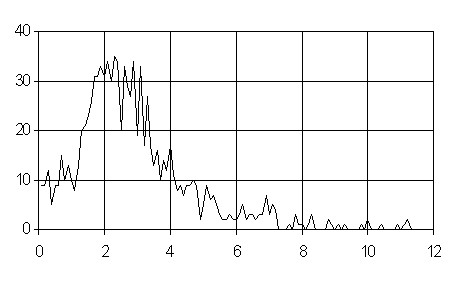
\includegraphics[width=0.8\textwidth]{figures/4_11.jpg}
  \caption{The distribution of problems of the class $G_{SH}$}
\end{figure}

\begin{figure}[h]
  \label{fig:4_12}
  \centering
  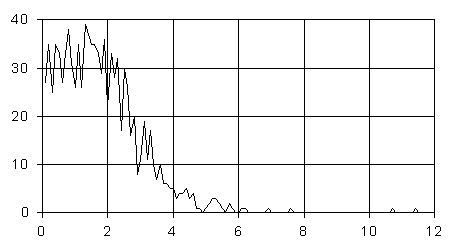
\includegraphics[width=0.8\textwidth]{figures/4_12.jpg}
  \caption{The distribution of problems of the class $G_{HL}$}
\end{figure}

The distribution of the interval lengths $[\alpha,\beta]$ from (4.41) including the solution points $x^*$ corresponding to the problems from the first set is presented in Fig. 4.11. Fig. 4.12 demonstrates a similar distribution for the problems of the second set. In these figures, the values $(\beta=\alpha)/(b-a)$ (in percentage) are plotted against the abscissa axes while the numbers of problems in the corresponding sets are plotted against the ordinate ones. In order to obtain the discussed estimates, the lengths of the intervals $[\alpha,\beta]$ corresponding to the respective functions were determined by a numerical method.

More detailed information on the number of problems (in either of two sets) featured by a small (less than 0.1\%) measure of the interval $[\alpha,\beta]$ is presented below.

\begin{table}
  \caption{The number of problems with a small measure of the interval $[\alpha,\beta]$}
\begin{center}
  \label{tab4:exp_results2}
  \begin{tabular}{| c | c | c | c| c | c | c | c | c| c |}
    \hline
    \% & 0.01 & 0.02 & 0.03 & 0.04 & 0.05 & 0.06 & 0.07 & 0.08 & 0.09 \\ \hline
    $G_{SH}$ & 0 & 1 & 2 & 1 & 0 & 0 & 1 & 1 & 1  \\ \hline
    $G_{HL}$ & 3 & 6 & 2 & 3 & 5 & 1 & 2 & 1 & 2 \\ \hline
  \end{tabular}
\end{center}
\end{table}

As follows from the figures and Table \ref{tab4:exp_results2}, the problems from the second set produced by generator $G_{HL}$ are characterized in general by a narrower feasible vicinity of the solution point $x^*$.

The constraint functions $g_\nu( x ),\: 1 \le\nu\le 5$, and the objective function $\varphi (x)$ for a problem from the class $G_{HP}$ are plotted in Fig. 4.13 as an example. The feasible domains which are formed by the separate constraints are marked on the abscissa axis. The whole feasible domain of the problem (the intersection of all feasible domains of the constraints) is shown along with the graph of the objective function.

\begin{figure}[h]
  \label{fig:4_13}
  \centering
  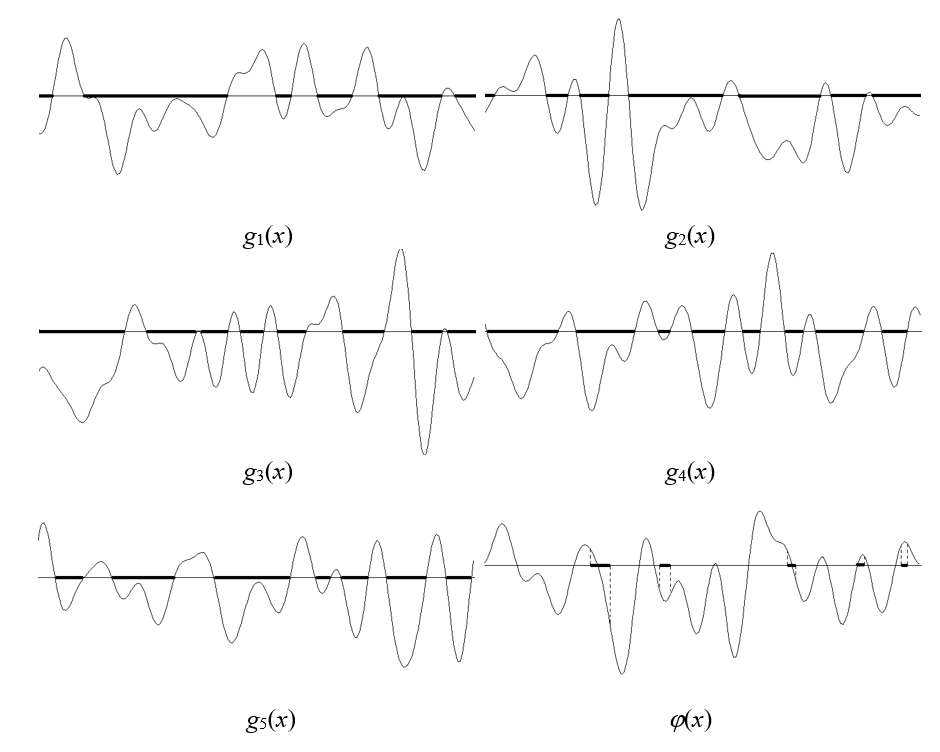
\includegraphics[width=0.8\textwidth]{figures/4_13.png}
  \caption{Function plots of a test problem from the class $G_{HL}$}
\end{figure}

The experiments have been carried out for the algorithms described above with the fixed constraints’ check order and with the adaptive one (FCOM and ACOM, respectively). The parameters $r_\nu, 1\le\nu\le 5$, from (4.17) were defined by the expressions
\begin{displaymath}
  r_\nu = \left\{
  \begin{array}{lr}
    \gamma, & k_\nu < 20\\
    2, & k_\nu \ge 20
  \end{array}
  \right.,
\end{displaymath}
where $k_\nu$ is the number of the calculated values of the function $g_\nu$ (i.e., the cardinality of the set $I_\nu$). In the experiments, the values $\gamma=20,\: \epsilon = 0.001$, and the reserves $\epsilon_\nu=0.1,\: 1\le\nu\le 5$, were set for the set produced by the generator $G_{SH}$. For the problems from the second set (generator $G_{HL}$ ) the values  $\gamma=10,\: \epsilon = 0.0001$, and the reserves $\epsilon_\nu=0.001,\: 1\le\nu\le 5$, were used.

\begin{figure}[h]
  \label{fig:4_14}
  \centering
  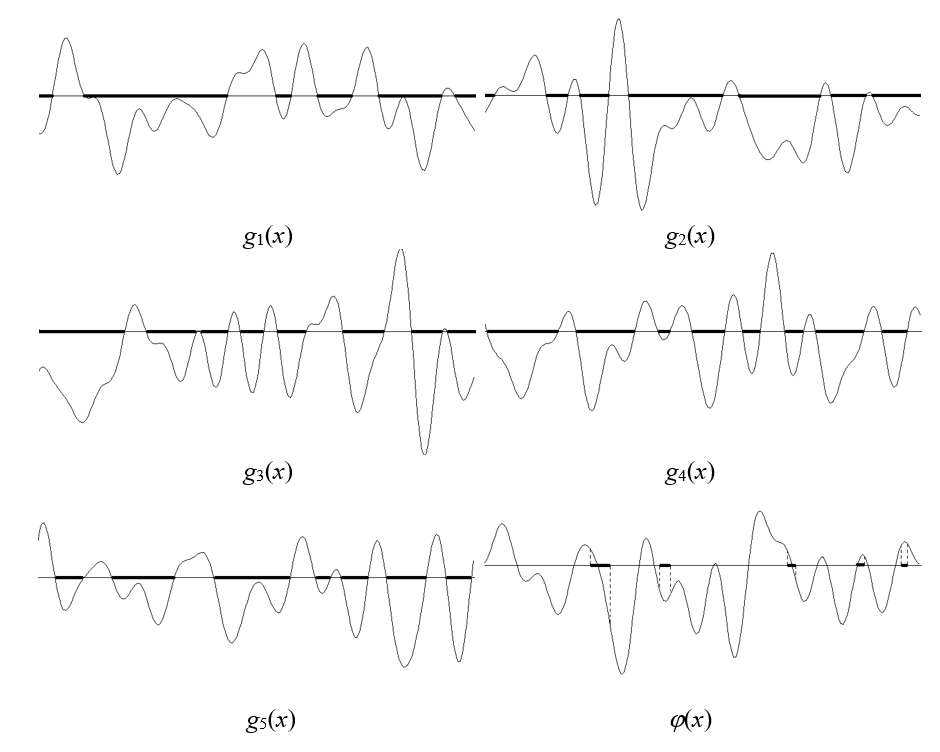
\includegraphics[width=0.8\textwidth]{figures/4_13.png}
  \caption{Operational characteristics for the class $G_{SH}$}
\end{figure}

\begin{figure}[h]
  \label{fig:4_15}
  \centering
  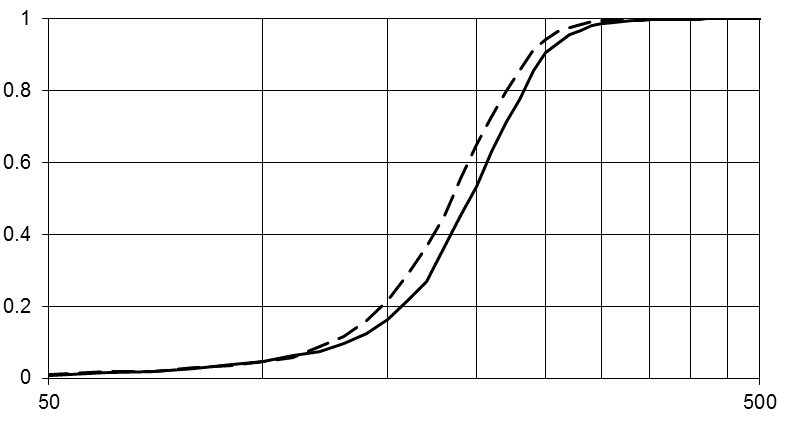
\includegraphics[width=0.8\textwidth]{figures/4_15.png}
  \caption{Operational characteristics for the class $G_{HL}$}
\end{figure}

The operational characteristics for both the methods obtained on the sets produced by generators $G_{SH}$ and $G_{HL}$ are presented in figures 4.14 and 4.15, respectively. The lower (solid) curves correspond to FCOM while the upper (dashed) ones --- to ACOM. These positions of the curves demonstrate that the algorithm with the adaptive check order provides in average faster obtaining the estimates falling into given vicinity of the solution than the algorithm with the fixed checking order.

\begin{figure}[h]
  \label{fig:4_16}
  \centering
  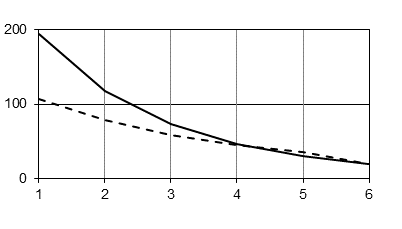
\includegraphics[width=0.8\textwidth]{figures/4_16.png}
  \caption{Average number of function values computations for the class $G_{SH}$}
\end{figure}

\begin{figure}[h]
  \label{fig:4_17}
  \centering
  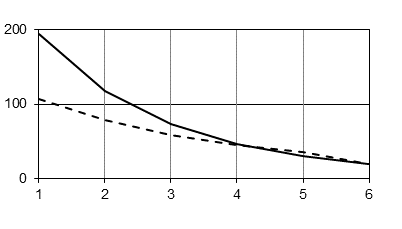
\includegraphics[width=0.8\textwidth]{figures/4_17.png}
  \caption{Average number of function values computations for the class $G_{HL}$}
\end{figure}

Moreover, the trials executed according to the rules of ACOM appear to be much less computation costly (in average) than the ones executed by FCOM. This fact is illustrated in figures 4.16 and 4.17, where the average number of computations of the function values executed by FCOM and ACOM for given sets are presented. Fig. 4.16 corresponds to the generator $G_{SH}$ while Fig. 4.17 shows the results for the generator $G_{HL}$. In both figures the function indices are plotted on the abscissa axes. The estimates of the average numbers of the computations of these function values during the trials’ execution are marked on the plot axes. The solid lines in the figures connect the points of the estimates corresponding to FCOM while the dashed ones connect the points of estimates corresponding to ACOM. The presented data confirm that introducing the adaptive constraints’ check order can reduce the total number of the computations essentially.

\section{Parallel computations for the multiextremal optimization problems with nonlinear constraints}
\subsection{Asynchronous parallel index algorithm}
In this subsection the asynchronous parallel index algorithm with $p>1$ parallel processors for solving the problem \eqref{ex4:problem} will be presented.

The first $p$ trial points are selected at the internal points of the interval $[a,b]$ arbitrarily. Each processor starts the trials execution at the corresponding points. After completing the $k^{th}$ trial, when the points $x^{k+1},\dots, x^{k+p - 1}$ have already been selected but the trial results at these points are not obtained yet, the point of the next trial $x^{k+p}$ is selected according to the following rules.

\emph{Rule 1.} Renumber the points of the preceding trials $x^1,\dots,x^k$ by the subscripts in the increasing order of the coordinate values, i.e.,
\begin{equation}
  \label{eq4:par_search_data}
  a=x_0<x_1<\dots x_i<\dots<x_{k+p-1}<x_{k+p}=b,
\end{equation}
the points $x_0=a$ and $x_{k + p}=b$ are included into series \eqref{eq4:par_search_data} additionally for the convenience of the future notation.

\emph{Rule 2.} Determine the set $I$ of the points $x_i,\: 1\le i<k+p$, such that the trials at these points have not been completed yet.

\emph{Rule 3.} Juxtapose to each point $x_i,\: 1\le i<k+p$, from series \eqref{eq4:par_search_data} such that $x_i\not\in I$ the
index $\nu=\nu(x_i)$ and the value $z_i=g_\nu(x_i )$ calculated at this point (the values $z_0$ and $z_{k + p}$ are not determined).

\emph{Rule 4.} Construct the sets
\begin{equation}
  I_\nu=\{i:1\le i<k+p, \nu=\nu(x_i),x_i\not\in I\},\:1\le\nu\le m+1,
\end{equation}
including the subscripts of all points $x_i ,1\le i<k+p$, with the same index, in which the trials are completed at the moment. The boundary points $x_0=a$ and $x_{k + 1}=b$ are considered as the points with the zero indices. The additional set $I_0=\{0,k+1\}$ is associated with these points.

Find the maximum value of the index
\begin{equation}
  M=\max\{\nu=\nu(x_i),x_i\not\in I,1\le i \le k\}.
\end{equation}

\emph{Rule 5.} Compute current estimates
\begin{equation}
  \label{eq4:lip_est_par}
  \mu = \max\left\{ \frac{\left|z_i-z_j\right|}{ x_i - x_j }, \; i,j \in I_\nu, \; i>j \right\},
\end{equation}
for the unknown Lipschitz constants $L_\nu$ of the functions $g_\nu,\: 1\le\nu\le m+1$. If the set $I_\nu$ includes less than two elements or if $\mu_\nu$ from \eqref{eq4:lip_est_par} appears to be equal to zero, to set $\mu_\nu=1$.

\emph{Rule 6.} For all nonempty sets $I_\nu,\: 1\le\nu\le m+1$ calculate the estimates
\begin{equation}
  \label{eq4:z_const_par}
  z_\nu^\ast = \left\{
  \begin{array}{lr}
    -\epsilon_\nu, & \nu < M,\\
    \min\{ g_\nu(y(x_i): i\in I_\nu \}, & \nu = M.
  \end{array}
  \right.
\end{equation}
where the vector $\epsilon_R=(\epsilon_1 ,\dots, \epsilon_m )$ is a given vector with the non-negative components (\emph{the reserve vector}).

\emph{Rule 7.} Compute the characteristics $R(i)$ for each interval $(x_{i-1}, x_i ),\: x_{i – 1}\not\in I,\: x_i\not\in I, 1\le i\le k+p$ where
\begin{gather}
  R(i)=2\Delta_i-4\frac{z_i-z_\nu^\ast}{r_\nu \mu_\nu}, \; \nu=\nu(x_i)>\nu(x_{i-1}), \nonumber \\
  \label{eq4:characteristic_par}
  R(i)=\Delta_i+\frac{(z_i-z_{i-1})^2}{r_\nu^2 \mu_\nu^2\Delta_i}-2\frac{z_i+z_{i-1}-2z_\nu^\ast}{r_\nu \mu_\nu}, \;  \nu=\nu(x_i)=\nu(x_{i-1}),\\
  R(i)=2\Delta_i-4\frac{z_{i-1}-z_\nu^\ast}{r_\nu \mu_\nu}, \; \nu=\nu(x_{i-1})>\nu(x_i), \nonumber \\
  \Delta_i=x_i - x_{i-1} \nonumber
\end{gather}
where the values $r_\nu>1,\: 1\le\nu\le m+1$ are the algorithm parameters and $\Delta_i=x_i-x_{i-1}$.

\emph{Rule 8.} Select the interval $(x_{t-1},x_t )$ whith the largest characteristic
\begin{equation}
  \label{eq4:MaxR_par}
  R(t)=\max\{R(i):x_{i-1}\not\in I,x_{i}\not\in I,1\le i\le k+p\}.
\end{equation}

\emph{Rule 9.} Execute the next trial at the middle point of the interval $(x_{t-1},x_t )$ if the indices of its boundary points are not the same, i.e.,
\begin{equation}
  \label{eq4:next_point_1_par}
  x^{k+1} = \frac{x_t + x_{t-1}}{2}, \; \nu(x_{t-1}) \neq \nu(x_t).
\end{equation}
Otherwise, accept
\begin{equation}
\label{eq4:next_point_2_par}
x^{k+p} = \frac{x_t+x_{t-1}}{2} - \frac{z_t-z_{t-1}}{2r_\nu\mu_\nu},\; \nu=\nu(x_{t-1})=\nu(x_t).
\end{equation}
as the point of the next trial.

The rules described above can be supplemented with the termination condition
\begin{equation}
\label{eq4:stop_cond_par}
  x_t - x_{t-1}\le\epsilon
\end{equation}
where $t$ from \eqref{eq4:MaxR_par} and $\epsilon>0$ is the predefined accuracy of the search.

\subsection{The convergence conditions of the algorithm}
\begin{theorem}
  \label{th4:convergence_par}
  Assume problem \eqref{eq4:problem} to have a solution $x^*$ and the following conditions to be fulfilled:
  \begin{itemize}
    \item each subdomain $Q_j ,1\le j\le m+1$ from \eqref{eq4:q} is a union of a finite number of positive length segments;
    \item each function $g_j ,1\le j\le m+1$ satisfies Lipschitz condition with the corresponding constant $L_j$;
    \item the components $\epsilon_\nu$ of the reserve vector $\epsilon_R$ satisfy the inequalities
    \begin{equation}
      \label{eq4:reserves_par}
      0<2\epsilon_\nu<L_\nu(\beta-\alpha)
    \end{equation}
    where $\beta-\alpha$ is the length of the interval $[\alpha,\beta]$ belonging to the feasible domain $Q$ from \eqref{eq4:Q_union} and including the point $x^*$ which is the solution of the problem;
    \item beginning from sufficiently large step number $k$, the values $\nu_\nu$ from \eqref{eq4:lip_est_par} corresponding to the nonempty sets $I_\nu$ satisfy the inequalities
    \begin{equation}
      r_\nu\mu_\nu>2L_\nu,\:1\le\nu\le m+1,
    \end{equation}
    where the algorithm parameters $r_\nu>1,\:1\le\nu\le m+1$;
    \item during the parallelization, the inequalities
    \begin{displaymath}
      T^j_{l+1}-T^j_j<T<\infty,1\le j\le p, l>1,
    \end{displaymath}
    are true where $T_l^j$ is the moment of completing the $l$ th trial by the $j^{th}$ processor and the inequality $1<p<P<\infty$ takes place for the number of processors $p$.
  \end{itemize}
  Then:
  \begin{itemize}
    \item the point $x^*$ is a limit one for the sequence ${x^k }$ generated by the described asynchronous algorithm for problem \eqref{eq4:problem} if $\epsilon=0$ in termination condition \eqref{eq4:stop_cond_par};
    \item any limit point $\overline x$ of the sequence $\{x_k \}$ is a solution of the problem \eqref{eq4:problem};
    \item the convergence to the limit point $\overline x$ is bilateral if $\overline x\not=a$ and $\overline x\not=b$.
  \end{itemize}
\end{theorem}

Before the proof of the theorem, let us formulate and prove several auxiliary statements.

\begin{lemma}
  (on the sequence of the shrinking intervals). Assume the conditions of Theorem \ref{th4:convergence_par} to be satisfied. Then for each limit point $x$ of the sequence $\{x_k\}$ there exists an infinite sequence of the intervals
  \begin{equation}
    \{(x_{t-1},x_t):t=t(q^s)\},\:s=1,2,\dots,
  \end{equation}
  satisfying the conditions
  \begin{gather}
    \overline x= \cap_{s=1}^\infty[x_{t-1},x_t], \\
    \lim_{p\to\infty}\Delta_t=0, \\
    R(t(q^s))>0,\:s=1,2,\dots, \\
    \lim_{p\to\infty}R(t(q^s))=0,
  \end{gather}
  where $q^1<q^2<\dots;\:R(t),\:\Delta_t$, and $t$ are from rules \eqref{eq4:characteristic_par} and \eqref{eq4:MaxR_par}, correspondingly.
\end{lemma}

\begin{proof}
  Since $\overline x$ is a limit point, there exists a sequence of the trial numbers $q^1,q^2,\dots$ satisfying the conditions
  \begin{equation}
    x^{q+1},\overline x\in[x_{t-1},x_t], t=t(q),q\in\{q^p\},p=1,2,\dots.
  \end{equation}
  These conditions reflect the fact that the point of the $(q+1)^{th}$ trial falls into the interval $[x_{t-1},x_t]$ containing the point $\overline x$ at the step $q$, i.e., $t=t(q)$.

  It follows from this condition, from the rules of the next trial point selection \eqref{eq4:next_point_1_par} and \eqref{eq4:next_point_2_par}, and from the estimate of the value $\mu_\nu$ from \eqref{eq4:lip_est_par}, that
  \begin{equation}
    \label{eq4:4_60}
    \max\{x_t-x^{q+1},x^{q+1}-x_{t-1}\}\le\gamma \Delta_t,
  \end{equation}
  where $\gamma=(r+1)/2r<1$ and
  \begin{equation}
    r=\min\{r_\nu:1\le\nu\le m+1\}>1.
  \end{equation}
  Then, the property (4.56) is a consequence of inequality \eqref{eq4:4_60}.

  At every step $k\ge 1$ there exists an interval $(x_{i-1},x_i), \:i=i(k)$, at one of the ends of which the value $z^*_\omega$ from \eqref{eq4:z_const_par} is achieved. This value corresponds to the index $\omega$ defined (when $\omega<m$) by the conditions $I_\omega\not=\O,\: I_{\omega+1}\not=\O$. If $I_{m+1}=\O$, the index $\omega=m+1$. If at that $\nu(x_{i -1} )\not = \nu(x_i )$, then according (4.47) and (4.50), $R(i)=2\Delta_i>0$. In the case when $\nu(x_{i -1} )= \nu(x_i )=\omega$, the estimate
  \begin{displaymath}
    \max(z_{i-1}, z_i)-z^*_\omega\le\mu\Delta_i
  \end{displaymath}
  follows from \eqref{eq4:lip_est_par} and, along with \eqref{eq4:characteristic_par}, gives the estimate
  \begin{displaymath}
    R(i)=\Delta_i\left(1-\frac{\max(z_{i-1},z_i)-z^*_\omega}{r_\omega\mu_\omega\Delta_i}\right)\ge (1-r^{-1})\Delta_i,
  \end{displaymath}
  where $r$ is from (4.61). Thus, at any search step $k\ge 1$ there exists an interval having a strictly positive characteristic. Hence, taking into account the rules of selection of the interval with the greatest characteristic \eqref{eq4:MaxR_par}, one can conclude that the intervals from system (4.54) should also have the positive characteristics since these ones undergo splitting up by the trial points falling into these intervals. Consequently, conditions (4.57) hold.

  It follows from the trial execution rules and condition (4.35) that for $\nu(x_i )\le m$ the values $z_i$ assigned to the points $x_i$ from \eqref{eq4:par_search_data} are positive. Therefore, according to \eqref{eq4:z_const_par},
  \begin{displaymath}
    z_i=g_\nu(x_i)\ge z^*_nu,\:1\le\nu=\nu(x_i)\le m+1,\: 0\le i\le k.
  \end{displaymath}
    Now from the rules \eqref{eq4:characteristic_par} for the characteristics and the limit (4.56), taking into account the condition \eqref{eq4:lip_condition} of Lipschitzness of the functions and inequality (4.57), one can derive out the truth of statement (4.58).
\end{proof}
\begin{lemma}
  (on the existence of a feasible point). Assume the conditions of Theorem \ref{th4:convergence_par} to be fulfilled. Then, there exists the trial index $h\ge 1$, for which
  \begin{equation}
    \label{eq4:62}
    \nu(x^h)=m+1.
  \end{equation}
\end{lemma}
\begin{proof}
  Let us assume the opposite and consider the interval $[x_{t-1},x_t]$ including the problem solution $x^*$ from \eqref{eq4:problem} at the step $k$, i.e., $t=t(k)$. Since we have assumed the equality \eqref{eq4:62} not to take place and, consequently, the sequence $\{x^k\}$ does not include the points from the feasible domain $Q$, the interval $[\alpha,\beta]$ from (4.52) should satisfy the conditions
  \begin{equation}
    x^*\in [\alpha,\beta]\subset[x_{t-1}, x_t].
  \end{equation}
  Then, from this condition as well as from the Lipschitz properties of the problem functions the relations
  \begin{gather}
    z_{t-1}\le L_\nu(\alpha - x_{t-1})\le L_\nu\Delta_t-L_\nu(\beta-\alpha),\:\nu=\nu(x_{t-1}) \\
    z_t\le L_\nu(x_{t}-\beta)\le L_\nu\Delta_t-L_\nu(\beta-\alpha),\:\nu=\nu(x_{t})
  \end{gather}
  follow. It was taken into account when deriving out of the above relations that
  \begin{displaymath}
    g_\nu(x)\le 0,\: x\in[\alpha,\beta]\subset Q.
  \end{displaymath}
  Analogously, the case $\nu=\nu(x_{t-1})=\nu(x_t)$ corresponds to the inequality
  \begin{equation}
    z_t+z_{t-1}\le L_\nu \Delta_t - L_\nu(\beta-\alpha).
  \end{equation}

  Now, from the characteristic rules \eqref{eq4:characteristic_par}, from inequalities (4.64)–(4.66), and from the inequality
  \begin{displaymath}
    z^*_\nu\ge-\epsilon_\nu
  \end{displaymath}
  resulting from \eqref{eq4:z_const_par} either the estimate
  \begin{displaymath}
    R(t)\ge\Delta_t(1-2L_\nu/r_\nu\mu_\nu)+2(L_\nu(\beta-\alpha)-2\epsilon_\nu)/r_\nu\mu_\nu,
  \end{displaymath}
  or the estimate
  \begin{displaymath}
    R(t)\ge\Delta_t(1-2L_\nu/r_\nu\mu_\nu)+4(L_\nu(\beta-\alpha)-2\epsilon_\nu)/r_\nu\mu_\nu,
  \end{displaymath}
  is true. Taking into account the third condition of Theorem \ref{th4:convergence_par} and the fourth one, in both cases we get the inequality
  \begin{equation}
    R(t(k))>0
  \end{equation}
  which holds for sufficiently large step numbers $k$.

  From (4.58), (4.67), and from the rule (4.48) determining the choice of the interval for the next trial point, the inevitability of carrying out a trial in the interval $[x_{t-1},x_t]$ from (4.63) follows. Consequently, the interval $[x_{t-1},x_t]$ will be divided into two subintervals. After that, at least one of those will include the point $x^*$. The repetition of this division generates (with $k\to\infty$) an infinite sequence of the subintervals shrinking to the point $x^*$ . In other words, if the third condition of Theorem \ref{th4:convergence_par} and the fourth one are satisfied, $x^*$ is the limit point of the sequence ${x^k}$.

  Since the coincidence $x^*$ with one of the trial points means (4.62) to hold, then it remains to consider the case when $x^*\in(x_{t- 1} ,x_t ),\: t=t(k)$ for any $k\ge 1$. Here, because of the first condition of Theorem \ref{th4:convergence_par} and the definition (4.31) either $[x_{t-1},x^*]\in Q$ or $[x^* ,x_t]\in Q$ if the number $k$ is sufficiently large. In this case, either $\nu(x_{t-1})=m+1$ or $\nu (x_t )=m+1.$
\end{proof}

\begin{lemma}
  on the feasibility of any limit point). Assume the conditions of Theorem \ref{th4:convergence_par} to be met. Then any limit point $\overline x$ of the sequence $\{x_k\}$ is feasible, i.e.,
  \begin{equation}
    \nu(\overline x)=m+1
  \end{equation}
\end{lemma}

\begin{proof}
  Let us assume the opposite. According to (4.55) and (4.56),
\end{proof}

\section*{A brief conclusion}
Constrained global optimization problems are under consideration. The method of penalty functions is one of the most popular numerical methods for solving the problems of this kind. Nevertheless, the method of penalty functions has a number of disadvantages. A new method for reduction of a constrained problem to an unconstrained one, so called \emph{index method}, has been considered in this chapter. This method, unlike the classical penalty function one, allows avoiding the problem of the parameter selection (like the penalty coefficients for the constraints). It is also allows solving the problems with partially defined objective function and constraints. This is quite natural for many applied problems, especially, in the optimal design of technical systems, because if some conditions of operation are not met, then some other characteristics of the system performance may not be defined.

The issues of convergence acceleration of the index method have been considered also. Two approaches for the convergence acceleration have been proposed. The first of them is based on concept of $\varepsilon$-reserved solution to the constrained problem. The role of $\varepsilon$-reserved solution in constrained global optimization problems is somewhat similar to the regularity requirements in classical nonlinear programming problems. The second approach is based on adaptive order of checking for constraints. In the index method, every iteration performed at the corresponding point of the search domain includes checking for constraints of the problem at this point. When a violation is discovered for the first time, the current iteration is stopped, and the next iteration is initiated. However, in Lipschitz optimization problems a constraint violated at a point of the search domain is also violated in a certain neighborhood of this point. In this case, to reduce the number of checks, it is expedient to begin iterations in the neighborhood of this point with checking for the violated constraint. Thus, the iteration can be completed at a lower cost.

For all proposed algorithms, the results of numerical experiments are presented. The results confirm the theoretical statements about convergence acceleration.

\end{document}

%%%%%%%%%%%%%%%%%%%%% author.tex %%%%%%%%%%%%%%%%%%%%%%%%%%%%%%%%%%%

%\documentclass[graybox]{svmult}
%
%\usepackage{mathptmx}       % selects Times Roman as basic font
%\usepackage{helvet}         % selects Helvetica as sans-serif font
%\usepackage{courier}        % selects Courier as typewriter font
%\usepackage{type1cm}        % activate if the above 3 fonts are
                            %% not available on your system
%%
%\usepackage{makeidx}         % allows index generation
%\usepackage{graphicx}        % standard LaTeX graphics tool
                             %% when including figure files
%\usepackage{multicol}        % used for the two-column index
%\usepackage[bottom]{footmisc}
%\usepackage{amsmath}
%\usepackage{multirow}
%\newcommand{\extr}{extr}
%
%\makeindex             % used for the subject index
                       %% please use the style svind.ist with
                       %% your makeindex program
%
%%%%%%%%%%%%%%%%%%%%%%%%%%%%%%%%%%%%%%%%%%%%%%%%%%%%%%%%%%%%%%%%%%%%%%%%%%%%%%%%%%%%%%%%%%
%
%\begin{document}

\title{Sequential and parallel algorithms for multidimensional multiextremal optimization based on the nested  scheme of dimensionality reduction}
\titlerunning{Nested  scheme of dimensionality reduction}
% Use \titlerunning{Short Title} for an abbreviated version of
% your contribution title if the original one is too long
\author{Vladimir A.Grishagin and Ruslan A.Israfilov}
% Use \authorrunning{Short Title} for an abbreviated version of
% your contribution title if the original one is too long
\institute{Vladimir A.Grishagin \at N.I.Lobachevsky State University, Gagarin Avenue 23, 603950 Nizhni Novgorod, Russia   \email{vagris@unn.ru}
\and Ruslan A.Israfilov \at N.I.Lobachevsky State University, Gagarin Avenue 23, 603950 Nizhni Novgorod, Russia 
\email{ruslan@israfilov.com}}
%
\maketitle


\abstract{The dimensionality reduction schemes occupy an important place among the complexity reduction approaches in the multiextremal optimization problems. In the present chapter, one of such schemes, namely, so called nested optimization scheme is considered. This scheme allows one to replace solving a multidimensional problem by solving a family of one-dimensional subproblems nested recursively. Along with a general reduction scheme, its implementation in combination with various global search algorithms is considered. The nested scheme has a considerable potential of parallelization since various one-dimensional parallel optimization algorithms, in particular, the characteristical ones can be applied for solving the internal one-dimensional subproblems. The asynchronism of the parallel computations originating from the recursive nesting of the subproblems is an integral part of the scheme to be considered.}

\section{General nested optimization scheme}
\label{sec:5_1}
Let us consider a nonlinear programming problem in the form 
\begin{equation}
\label{eq:5_1}
\varphi(y)\rightarrow min,y\in Q\subseteq R^N,
\end{equation}
\begin{equation}
\label{eq:5_2}
Q=\{y\in D:g_j(y)\leq 0,\:1\leq j\leq m\},
\end{equation}
\begin{equation}
\label{eq:5_3}
D=\{y\in R^N:a_i\leq y\leq b_i,\:1\leq i\leq N\}.
\end{equation}

Assume that all constraint functions $g_j(y),\:1\leq j\leq m$,  are continuous and the domain $D$  is  bounded that provides the compactness of the feasible domain $Q$. 

Let us introduce a continuous function $G(y)$  defined in the domain $D$  such that
\begin{equation}
\label{eq:5_4}
  \begin{cases}
    G(y)\leq 0, & y\in Q, \\
    G(y)>0, & y\notin Q.
  \end{cases}
\end{equation}

For example, the following functions can be taken as $G(y)$ :
\begin{equation}
\label{eq:5_5}
G(y)=\max\{g_1(y),\;g_2(y),\:\ldots\:,g_m(y)\}
\end{equation}
or
\begin{equation}
\label{eq:5_6}
G(y)=\max\{0;\:g_1(y),\;g_2(y),\:\ldots\:,g_m(y)\}.
\end{equation}
The latter function equals to zero at all points of the domain $Q$.

The following notations
\begin{equation}
\label{eq:5_7}
u_i=(y_1,\ldots,\:y_i),\;v_i=(y_{i+1},\ldots,y_N),
\end{equation}
allow one to write down the vector $y$ as a pair $y=(u_i,\;v_i)$  for $1\leq i\leq N$. Assume that $y=v_0$  if $i=0$  and $y=u_n$  for $i=N$.

Let us introduce  \textit{sections} of the domain $Q$ as
\begin{equation}
\label{eq:5_8}
S_1=Q,\ S_{i+1}(u_i)=\{v_i\in R^{N-i}:(u_i,v_i)\in Q\},\:1\leq i\leq N-1,
\end{equation}
and \textit{projections}
\begin{equation}
\label{eq:5_9}
\Pi_{i+1}(u_i)=\{y_{i+1}\in R^1:\exists (u_{i+1},v_{i+1})\in S_{i+1}(u_i)\},\:1\leq i\leq N-1,
\end{equation}
of the sections $S_{i+1}(u_i)$ onto the axis $y_{i+1}$.

Let us define recursively a family of functions
\begin{equation}
\label{eq:5_10}
  \begin{cases}
    G^N(y)\equiv G(y), \\
    G^i(u_i)=\min\{G^{i+1}(u_i,y_{i+1}:y_{i+1}\in [a_{i+1},b_{i+1}]\},\;1\leq i\leq N-1,
  \end{cases}
\end{equation}
over corresponding projections 
\begin{equation}
\label{eq:5_11}
D_i=\{u_i\in R^i:y_j\in[a_j,b_j],\:1\leq j\leq i\}
\end{equation}
of the domain $D$  from (\ref{eq:5_3}) onto the coordinate axes $y_1,\ldots,y_i$. Moreover, by definition, $D_N=D$.

Because of the continuity of the function $G^N(y)\equiv G(y)$ and of the compactness of the domain $D$ the function  $G^{N-1}(u_{N-1})$ exists and is continuous in  $D_{N-1}$. This fact causes the existence and the continuity of the function  $G^{N-2}(u_{N-2})$ in  $D_{N-2}$ and further determines the existence and the continuity of all functions from family (\ref{eq:5_10}) in corresponding domains (\ref{eq:5_11}). 

The following lemma takes place.
\begin{lemma} 
\label{lem:5_1}
\begin{equation}
\label{eq:5_12}
G^i(u_i)=\min\{G(u_i,v_i):y_j\in [a_j,b_j],\:i+1\leq j\leq N\}.
\end{equation}
\end{lemma}
\begin{proof}
As a consequence of (\ref{eq:5_10}) the assertion (\ref{eq:5_12}) is equivalent to
\begin{equation}
\label{eq:5_13}
\min_{y_{i+1}\in [a_{i+1},b_{i+1}]}\ldots \min_{y_N\in [a_N,b_N]}G(u_i,v_i)=\min\{G(u_i,v_i):y_j\in [a_j,b_j],i+1\leq j\leq N\}.
\end{equation}

Because of the continuity of $G(y)$, for any $u_i\in D_i$ there exists $\bar{v}_i=(\bar{y}_{i+1},\ldots,\bar{y}_N)$ such that $\bar{y}_j\in [a_j,b_j],\:i+1\leq j\leq N,$ and
\begin{displaymath}
\min_{y_{i+1}\in [a_{i+1},b_{i+1}]}\ldots \min_{y_N\in [a_N,b_N]}G(u_i,v_i)=G(u_i,\bar{v}_i)
\end{displaymath}
from where it follows that the left-hand side of the equality  (\ref{eq:5_13}) is greater or equal to the right-hand side. 

Now the subject of our interest is the reverse inequality. Because of the continuity of $G(y)$ and of the compactness of the domain $D$  there exists a vector $v_i^*=(y_{i+1}^*,\ldots ,y_N^*)$  such that 
\begin{displaymath}
G(u_i,v_i^*)=\min\{G(u_i,v_i):y_j\in [a_j,b_j],\:i+1\leq j\leq N\}.
\end{displaymath}

According to (\ref{eq:5_10}), we have
\begin{displaymath}
G^{N-1}(u_i,y_{i+1}^*,\ldots ,y_{N-1}^*)=\min\{G(u_i,y_{i+1}^*,\ldots,y_{N-1}^*,y_N):y_N\in [a_N,b_N]\}\leq G(u_i,v_i^*),
\end{displaymath}
\begin{displaymath}
G^{N-2}(u_i,y_{i+1}^*,\ldots ,y_{N-2}^*)=\min\{G^{N-1}(u_i,y_{i+1}^*,\ldots,y_{N-2}^*,y_{N-1}):y_{N-1}\in [a_{N-1},b_{N-1}]\}\leq 
\end{displaymath}
\begin{displaymath}
\leq G^{N-1}(u_i,y_{i+1}^*,\ldots,y_{N-2}^*,y_{N-1}^*)\leq G(u_i,v_i^*),
\end{displaymath}
$\ldots$
\begin{displaymath}
G^i(u_i)=\min\{G^{i+1}(u_i,y_{i+1}):y_{i+1}\in [a_{i+1},b_{i+1}]\}\leq G^{i+1}(u_i,y_{i+1}^*)\leq G(u_i,v_i^*).
\end{displaymath}
This chain of inequalities finalizes the proof.
\end{proof}

Let us introduce the projections 
\begin{equation}
\label{eq:5_14}
Q_i=\{u_i\in R^i:\exists (u_i,v_i)\in Q\},\:1\leq i\leq N,
\end{equation}
of the domain $Q$ onto the coordinate axes $y_1,\ldots,y_i$.
\begin{lemma} 
\label{lem:5_2}
Projection (\ref{eq:5_14}) can be presented in the equivalent form 
\begin{equation}
\label{eq:5_15}
Q_i=\{u_i\in R^i:G^i(u_i)\leq 0\}.
\end{equation}
\end{lemma}
\begin{proof}
Let  (\ref{eq:5_14}) be fulfilled, i.e., for some $u_i$  there exists $v_i^*$  such that $(u_i,v_i^*)\in Q$. Then, $G(u_i,v_i^*)\leq 0$ , i.e., as a consequence of Lemma \ref{lem:5_1},
\begin{displaymath}
G^i(u_i)=\min\{G(u_i,v_i):y_j\in[a_j,b_j],\:i+1\leq j\leq N\}\leq G(u_i,v_i^*)\leq 0,
\end{displaymath}
and (\ref{eq:5_15}) is true.

Now assume that $G^i(u_i)\leq 0$  for some $u_i\in Q_i$. However, according to Lemma \ref{lem:5_1}, a vector $v_i^*$  exists such that $G^i(u_i)=G(u_i,v_i^*)\leq 0$ , i.e., $(u_i,v_i^*)\in Q$.

Lemma has been proved.
\end{proof}
\begin{lemma} 
\label{lem:5_3}
The definition of the projection (\ref{eq:5_9}) is equivalent to the form 
\begin{equation}
\label{eq:5_16}
\Pi_{i+1}(u_i)=\{y_{i+1}\in [a_{i+1},b_{i+1}]:G^{i+1}(u_i,y_{i+1})\leq 0\}.
\end{equation}
\end{lemma}
\begin{proof}
First of all, note that because of $Q\subseteq D$, for all $y\in Q$ the double inequalities $a_j\leq y_j\leq b_j$,  , hold necessarily. Let $y_{i+1}$  be such that $G^{i+1}(u_i,y_{i+1})\leq 0$ . Then there exists $v_{i+1}^*$  such that $G(u_i,y_{i+1},v_{i+1}^*)=G^{i+1}(u_i,y_{i+1})\leq 0$, i.e., $(y_{i+1}, v_{i+1}^*)\in S_{i+1}(u_i)$. Consequently, $y_{i+1}$  belongs to the projection $\Pi_{i+1}(u_i)$  in the sense of the definition (\ref{eq:5_9}).

Next, for any $y_{i+1}$  satisfying (\ref{eq:5_9}) there exists $v_{i+1}^*$  such that $(y_{i+1},v_{i+1}^*)\in S_{i+1}(u_i)$. Then, the vector $(u_i,y_{i+1},v_{i+1}^*)\in Q$, i.e., $G^{i+1}(u_i,y_{i+1})\leq G(u_i,y_{i+1},v_{i+1}^*)\leq 0$.

The equivalence of (\ref{eq:5_9}) and (\ref{eq:5_16})  has been proved.
\end{proof}
Now consider  a continuous function $\varphi(y)$. Setting $\varphi^N(y)\equiv \varphi(y)$ by definition, let us construct a family of functions 
\begin{equation}
\label{eq:5_17}
\varphi^i(u_i)=\min\{\varphi^{i+1}(u_i,y_{i+1}):y_{i+1}\in \Pi_{i+1}(u_i)\},\:1\leq i\leq N-1,
\end{equation}
defined over the corresponding projections $Q_i$  from (\ref{eq:5_14}). Then, according to \cite{5_CarrHowe} and \cite{5_StrSergMon2000} the basic relation of the nested optimization scheme 
\begin{equation}
\label{eq:5_18}
\min_{y\in Q}\varphi(y)=\min_{y_1\in \Pi_1}\min_{y_2\in \Pi_2(u_1)}\ldots\min_{y_N\in \Pi_N(u_{N-1})}\varphi(y).
\end{equation}
takes place. 

As it follows from (\ref{eq:5_18}), in order to solve the problem (\ref{eq:5_1})--(\ref{eq:5_3}) it is sufficient to solve the one-dimensional problem 
\begin{equation}
\label{eq:5_19}
\varphi^1(y_1)\rightarrow \min,\:y_1\in \Pi_1\subseteq R^1,
\end{equation}
\begin{displaymath}
\Pi_1=\{y_1\in [a_1,b_1]:G^1(y_1)\leq 0\}.
\end{displaymath}

According to (\ref{eq:5_17}), each calculation of the function $\varphi^1(y_1)$  at some fixed point $y_1\in\Pi_1$   requires solving  the one-dimensional problem 
\begin{displaymath}
\varphi^2(y_1,y_2)\rightarrow \min,\:y_2\in \Pi_2(y_1)\subseteq R^1,
\end{displaymath}
\begin{displaymath}
\Pi_2(y_1)=\{y_2\in [a_2,b_2]:G^2(y_1,y_2)\leq 0\}.
\end{displaymath}
This problem is a one-dimensional minimization problem with respect to $y_2$  since $y_1$  is fixed.

In turn, each calculation of the function $\varphi^2(y_1,y_2)$  with fixed $y_1,y_2$ generates solving the one-dimensional problem
\begin{displaymath}
\varphi^3(u_2,y_3)\rightarrow \min,\:y_3\in \Pi_3(u_2)\subseteq R^1,
\end{displaymath}
etc., up to solving the univariate problem 

\begin{equation}
\label{eq:5_20}
\varphi^N(u_{N-1},y_N)\rightarrow \min,\:y_N\in \Pi_N(u_{N-1})\subseteq R^1,
\end{equation}
where $u_{N-1}$  is fixed.

Thus, solving the problem (\ref{eq:5_1})--(\ref{eq:5_3}) can be reduced to solving a family of «nested» one-dimensional subproblems 
\begin{equation}
\label{eq:5_21}
\varphi^i(u_{i-1},y_i)\rightarrow \min,\:y_i\in \Pi_i(u_{i-1}),
\end{equation}
where the fixed vector $u_{i-1}\in Q_{i-1}$.

Solving initial multidimensional problem (\ref{eq:5_1})--(\ref{eq:5_3})  through solving the system of the one-dimensional subproblems (\ref{eq:5_21}) is called \textit{the nested optimization scheme}.

On the base of the nested scheme (\ref{eq:5_18}) many multidimensional optimization algorithms have been designed (see, for example, \cite{5_CarrHowe, 5_Evtushenko, 5_GerGriIsr, 5_GriIsrAIP, 5_GriIsrCEUR, 5_GrishaginStrongin_EnginCybernetics, 5_Piyavskij, 5_SergGriJCAA, 5_ShiOlaf, 5_StrSergMon2000, 5_vanDam}). This scheme has essential potential for constructing new optimization techniques by means of combining with different one-dimensional algorithms for solving the subproblems (\ref{eq:5_21}) (for example, characteristical methods \cite{5_GrishaginSergeyevStrongin} including information    algorithms \cite{5_SergeyevLocTun, 5_Sergeyev1998, 5_SergeyevGrishaginOMS, 5_SergMukhKvasLera, 5_StrMonRus, 5_Str1973, 5_StrMarkin, 5_StrSergMon2000}, methods by Piyavskij and Shubert \cite{5_Piyavskij, 5_Shubert} and Kushner \cite{5_Kushner}, Bayesian algorithms \cite{5_Locatelli, 5_Mockus1980, 5_Mockus1988, 5_MockusEddy_et_al, 5_Zilinskas1975, 5_Zilinskas1981, 5_Zilinskas1985}, etc.) 

As an illustration, let us consider an example of using the nested optimization scheme for the maximization of a two-dimensional multiextremal function 
\begin{equation}
	\label{eq:5_GriFun}
	\varphi(y)=\left\{\left(\sum _{i=1}^7\sum _{j=1}^7A_{ij} g_{ij} (y)+B_{ij}h_{ij}(y) \right)^2 +\left(\sum _{i=1}^7\sum _{j=1}^7C_{ij}g_{ij}(y)-D_{ij}h_{ij}(y)\right)^2 \right\}^{1/2},
	\end{equation}
	where 
	\begin{equation*}
	y=(y_1 ,y_2 )\in R^2 ,0\le y_s \le 1,s=1,2,
	\end{equation*}
	\begin{equation*}
	g_{ij} (y)=\sin (i\pi y_1 )\sin (j\pi y_2 ),
	\end{equation*}
	\begin{equation*}
	h_{ij} (y)=\cos (i\pi y_1 )\cos (j\pi y_2 )
	\end{equation*}
	 and the coefficients $A_{ij} ,B_{ij} ,C_{ij} ,D_{ij} $ are distributed uniformly over the interval $[-1,1]$.   

 The level curves of the objective function are shown  in Fig. \ref{fig:5_2}.  For this function the global maximum value 13.51 is located at the point (0.603, 0.408). Fig. \ref{fig:5_2}contains also the coordinates of the search trials generated by the nested scheme with the information core global search algorithm  applied for solving the one-dimension subproblems (\ref{eq:5_21}).
\begin{figure}[t]
\centering
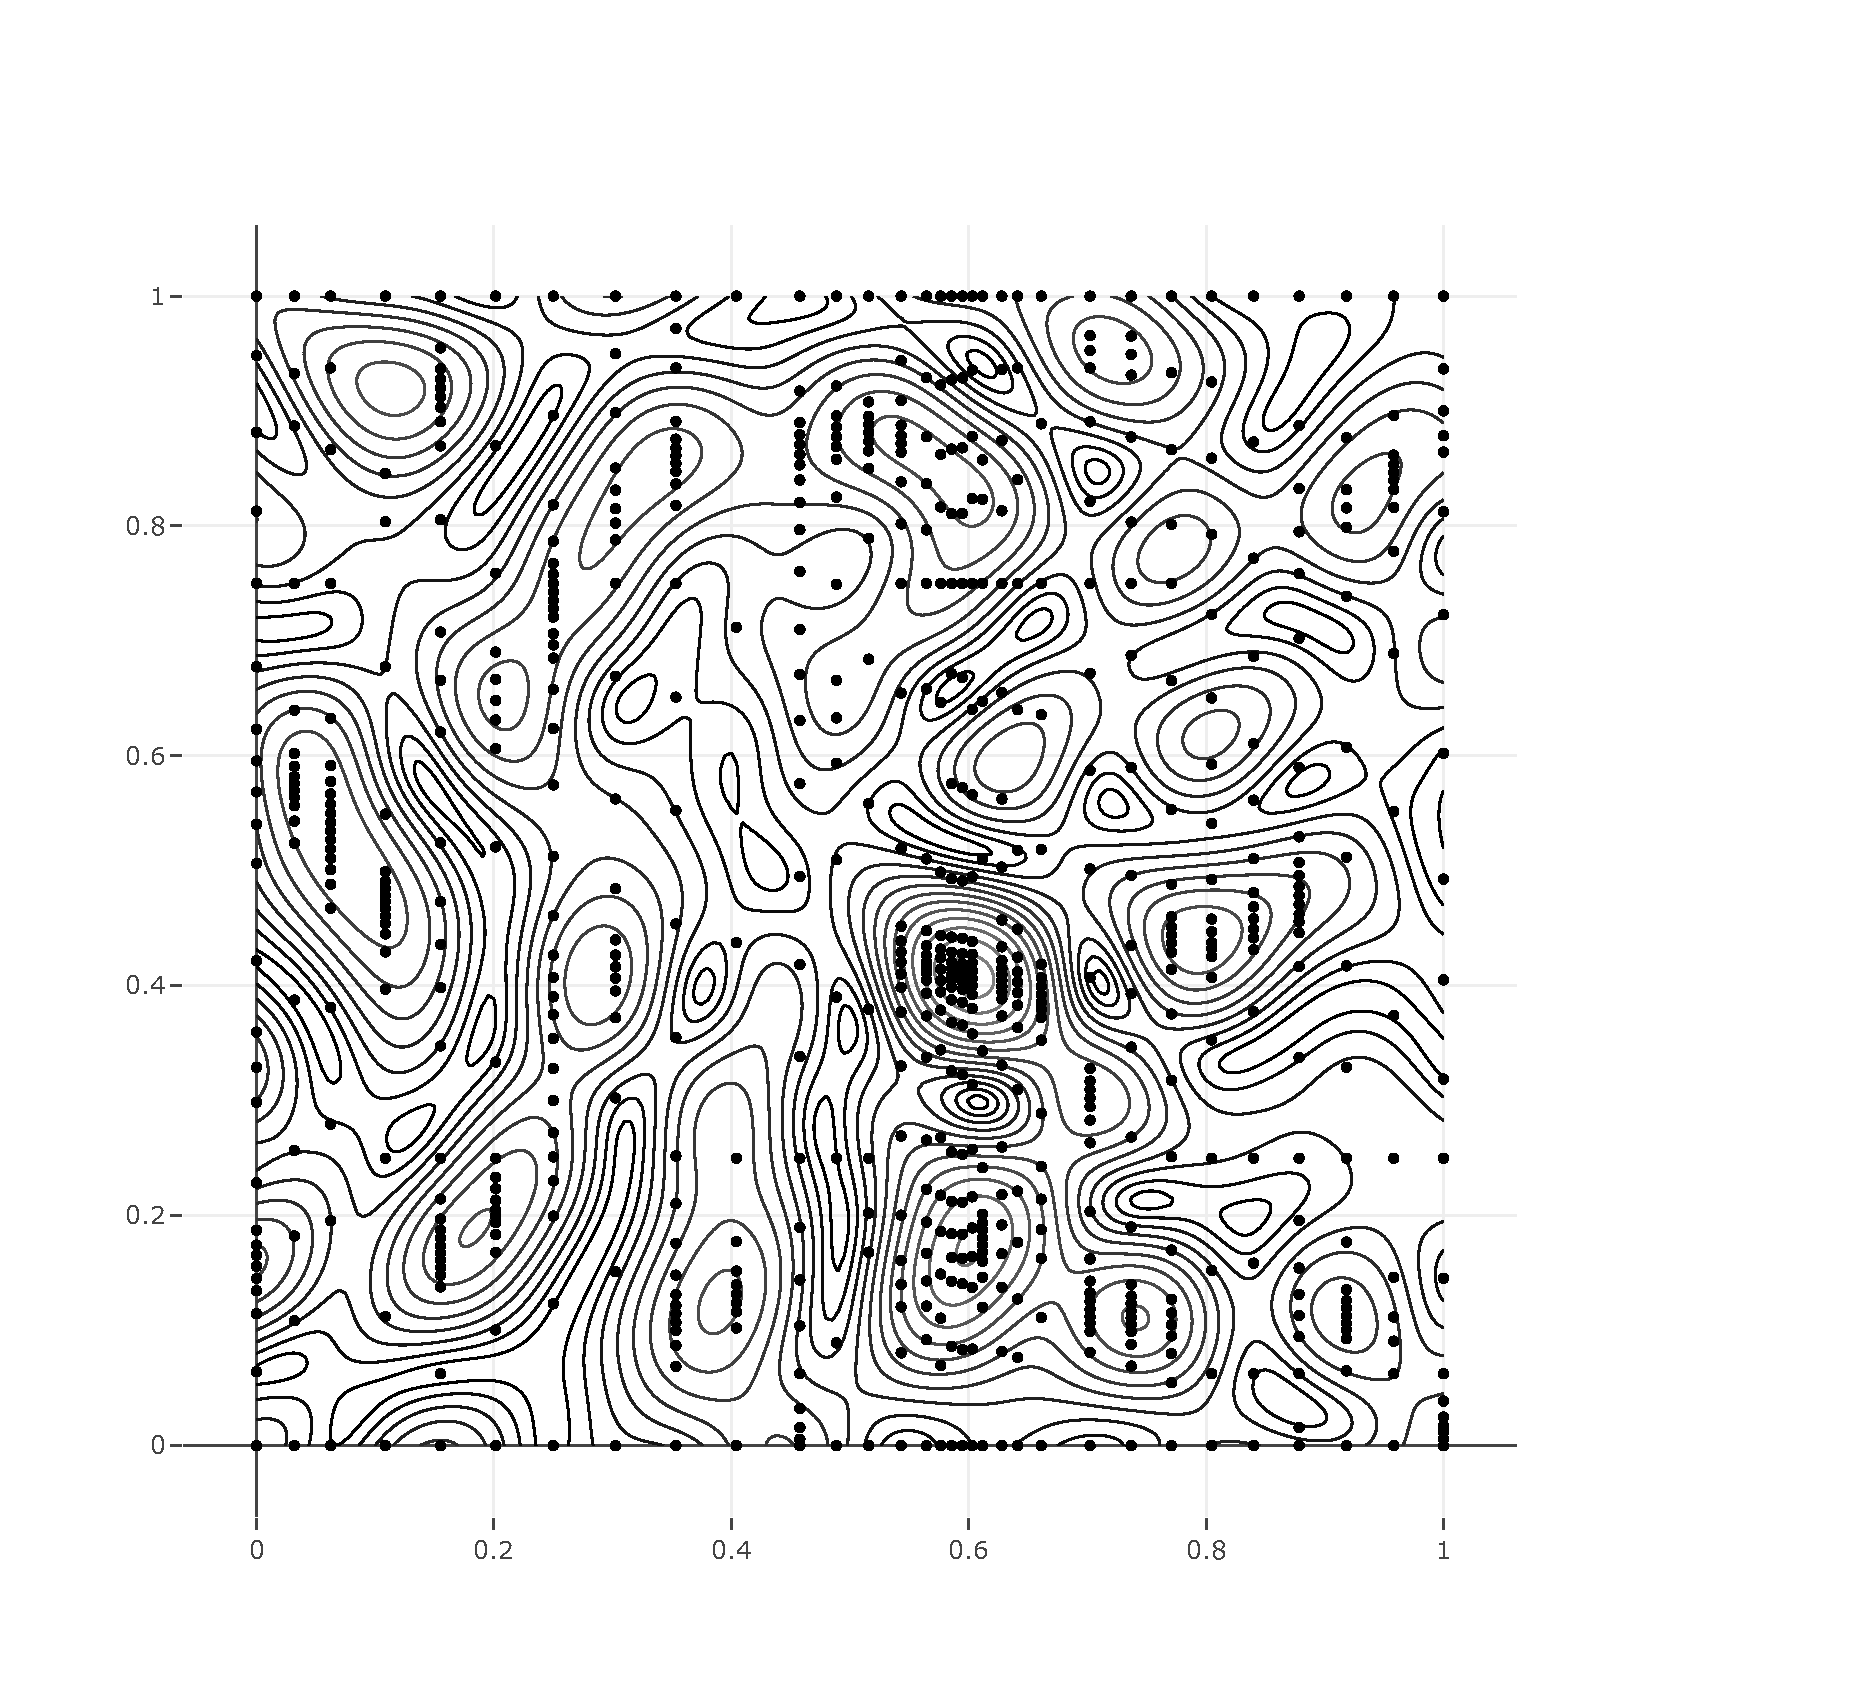
\includegraphics[width=1.1\linewidth]{figures/figure_5_2.pdf}
\caption{Level curves and trial points}
\label{fig:5_2}    
\end{figure}

The nested scheme (\ref{eq:5_18})--(\ref{eq:5_21}) may be generalized in the following way. Let us consider for simplicity a problem (\ref{eq:5_1}) without functional constraints, i.e., $Q=D$, and present the feasible domain  as the direct product of subdomains with smaller dimensions
\begin{displaymath}
D=D_1\times D_2\times\:\ldots\: D_s,\:1\leq s<N,
\end{displaymath}
where the subdomains $D_i,\:1\leq i\leq s,$ are hyperparallelepipeds (\ref{eq:5_3}) of corresponding dimensions $d_i$ such that $1\leq d_i<N$ and $\sum_{i=1}^s{d_i}=N$.

In this case (\ref{eq:5_18}) can be transformed to the form
\begin{displaymath}
\min_{y\in Q}\varphi(y)=\min_{z_1\in D_1}\min_{z_2\in D_2}\ldots\min_{z_s\in D_s}\varphi(y),
\end{displaymath}
where $z_1=u_{\sigma(1)},\:z_i=(y_{\sigma{(i-1)}}+1,\ldots, y_{\sigma(i)}),\:2\leq i\leq s,$ and $\sigma(j)=\sum_{i=1}^j{d_i},\:1\leq j\leq s$.

Then, instead of the family (\ref{eq:5_21}) we can solve the set of nested subproblems 
\begin{displaymath}
\varphi(u_{\sigma(i-1)},z_i)\rightarrow \min,\;z_i\in D_i,
\end{displaymath}
which can be multidimensional with lesser dimensions. Such approach was developed (see \cite{5_BarkGer2014, 5_BarkGerLeb, 5_BarkLeb, 5_SysoyevBarkGerLeb}) in combination with the optimization algorithms based on the Peano space-filling curves for solving the nested multidimensional subproblems.

Moreover, in the family (\ref{eq:5_21}) for several functions $\varphi^i(u_i)$ one can use the operation of taking maximum instead of minimum. In this case it is possible to calculate complex minmax (or maxmin) expressions. 

\section{Properties of one-dimensional subproblems in the nested optimization scheme}
\label{sec:5_2}
While analyzing univariate subproblems (\ref{eq:5_21}) of the nested scheme, two main problems arise:
\begin{description} [a)]
\item [a)] {the necessity to construct the feasible domains $\Pi_i(u_{i-1})$  for the one-dimensional search;}
\item [b)] {it is required to provide the minimization of the one-dimensional functions $\varphi^i(u_{i-1},y_i)$  in the domains  $\Pi_i(u_{i-1})$.}
\end{description}

The structure and the complexity of the projections $\Pi_i(u_{i-1})$  are completely determined by the complexity of the multidimensional feasible domain $Q$. The complexity of the second problem depends on the characteristics of the functions $\varphi^i(u_i)$ . These characteristics are influenced by the properties of the objective function $\varphi(y)$ as well as by the features of the search domain $Q$ defined by constraints (\ref{eq:5_2}) and (\ref{eq:5_3}).

\subsection {Structure of the feasible domains of the one-dimensional search}
\label{subsec:5_2_1}
The results of Lemma \ref{lem:5_3}, which has established the equivalence of Definition (\ref{eq:5_9}) and representation (\ref{eq:5_16}) enable to analyze the structure of the domains $\Pi_i(u_{i-1})$. In fact, (\ref{eq:5_16}) provides a constructive apparatus for building the domains $\Pi_i(u_{i-1})$  by means of finding the domains of the non-positivity for the functions $G^i(u_{i-1},y_i)$.

Since the function $G(y)$ is assumed to be continuous in the domain $D$, the functions $G^i(u_i)$ are continuous in $D_i$  from (\ref{eq:5_11}) and, therefore, with regard to $y_i\in [a_i,b_i]$  as well. Then, with fixed $u_{i-1}\in D_{i-1}$  each one-dimensional problem (\ref{eq:5_21}) can be rewritten in a unified form
\begin{equation}
\label{eq:5_22}
  \begin{cases}
    \bar{\varphi}(x)\rightarrow\min,\;x\in\bar{Q}\subseteq R^1, \\
    \bar{Q}=\{x\in[a,b]:g(x)\leq 0\},
  \end{cases}
\end{equation}
where the function $g(x)$ is continuous.

The continuity of the constraint $g(x)$ allows one to state that the feasible domain $\bar{Q}$  can be presented as a system of closed intervals
\begin{equation}
\label{eq:5_23}
\bar{Q}=\bigcup_{j=1}^q{[a^j,b^j]},
\end{equation}
where in each interval the function $g(x)$ is non-positive. 

As an example, let us consider the possible cases of the behavior of a continuous function generating the domains of the non-positivity presented in Fig. \ref{fig:5_3}. The corresponding intervals  are marked with  the signs $\times$  on the abscissa axis including the point of tangency. The right-side interval marked with $\times$ corresponds to the case when the function equals to zero over the interval of non-zero length. 
\begin{figure}[t]
\centering
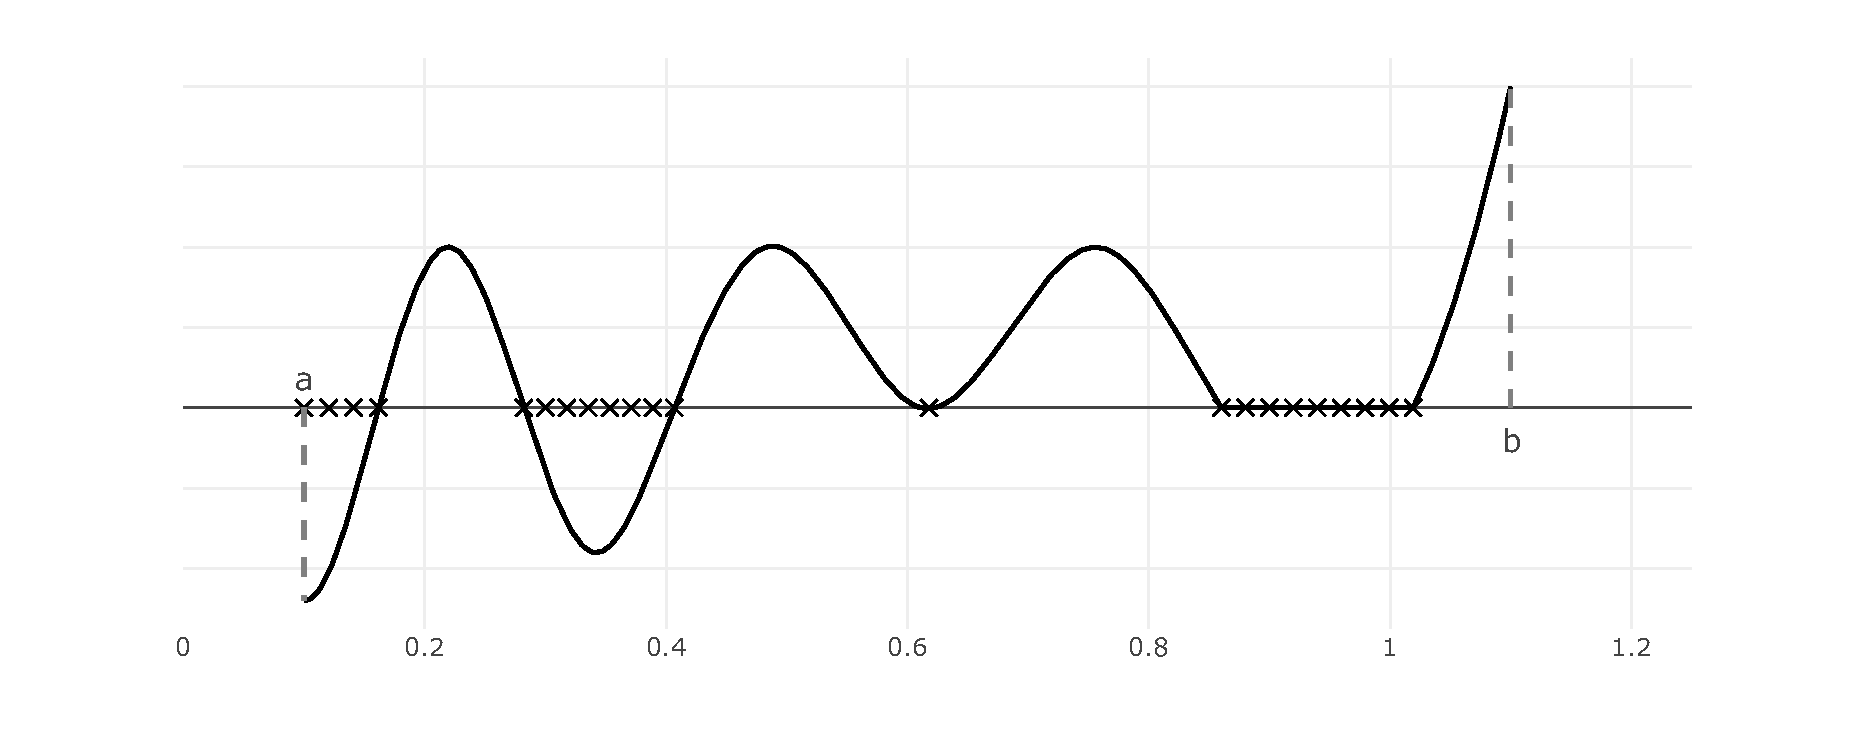
\includegraphics[width=1.1\linewidth]{figures/figure_5_3.pdf}
\caption{Domains of the non-positivity of a continuous function}
\label{fig:5_3}    
\end{figure}
In the system (\ref{eq:5_23}) the number of intervals $q$ can be infinite. As an example of such situation the function
\begin{displaymath}
g(x)=
  \begin{cases}
    x\sin(\frac{1}{x}), & x>0,\\
    0, & x=0.
  \end{cases}
\end{displaymath}
within the closed interval $[0,1]$ can be considered.

Thus, in the case of a continuous function $G(y)$, the projection $\Pi_i(u_{i-1})$ determined as  (\ref{eq:5_16}) is a set of the kind (\ref{eq:5_23}), i.e.,
\begin{equation}
\label{eq:5_24}
\Pi_i(u_{i-1})=\bigcup_{j=1}^{q_i}{[a_i^j,b_i^j]},
\end{equation}
where, in general, the number of the intervals $q_i$  and their boundaries $a_i^j$, $b_i^j$, $1\leq j\leq q_i,$ depend on the vector $u_{i-1}$ , i.e.,
\begin{equation}
\label{eq:5_25}
q_i=q_i(u_{i-1}),\:a_i^j=a_i^j(u_{i-1}),\:b_i^j=b_i^j(u_{i-1}).
\end{equation}

If the domain $Q$  is such that it is possible to obtain the explicit (analytical) expressions for the values $q_i,a_i^j,b_i^j$   as  functions of $u_{i-1})\in Q_{i-1}$  for all $1\leq i\leq N$, then the domain $Q$ is called \textit{the domain with the computable boundaries}. In particular, it is possible if all the roots of the functions $G^i(u_{i-1},y_i)$  with regard to the variables $y_i$  can be analytically found.
\begin{example}
\label {exam:5_1}
As the problem to be investigated  the problem (\ref{eq:5_1})--(\ref{eq:5_3}) with 
\begin{equation}
\label{eq:5_26}
  \begin{cases}
    \varphi(y)=y_1^2+y_2^2,\\
   Q=\{y\in D:(y_1-1)^2+(y_2-1)^2-1\leq 0\}, \\
	D=\{y\in R^2:0\leq y_1,y_2\leq 2\}
  \end{cases}
\end{equation}
is considered. The feasible domain is marked with gray in Fig. \ref{fig:5_4}. Also, the level curves of the objective function are shown there. In this problem, the function $G^2(y)=(y_1-1)^2+(y_2-1)^2-1$. It is evident that the function  $G^1(y_1)=\min\{G^2(y_1,y_2):y_2\in [0,\;2]\}=(y_1-1)^2-1$. 
\begin{figure}[t]
\centering
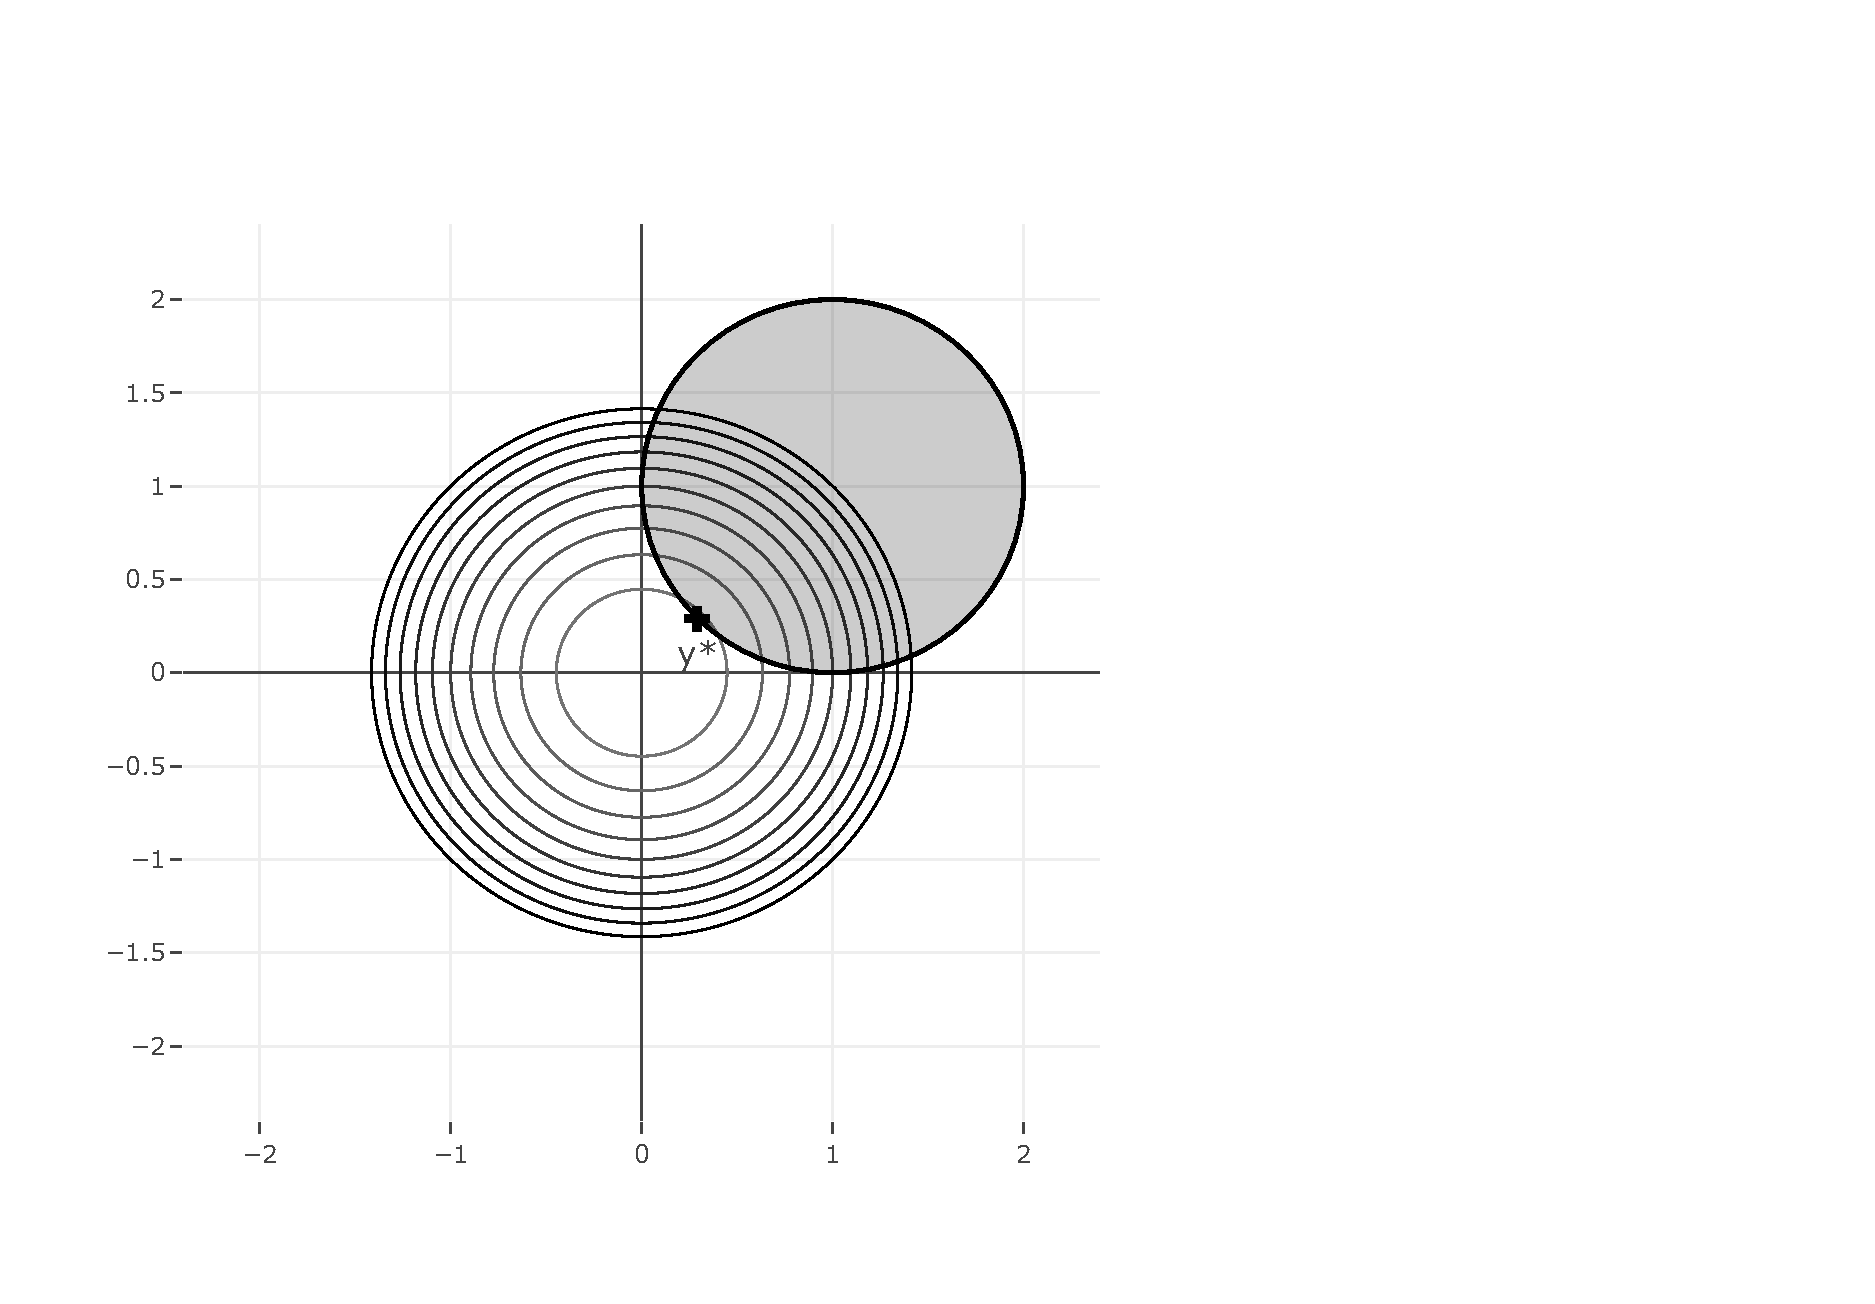
\includegraphics[width=1.1\linewidth]{figures/figure_5_4.pdf}
\caption{Feasible domain and level curves of the objective function}
\label{fig:5_4}    
\end{figure}

According to (\ref{eq:5_16}), the domains where the functions $G^1(y_1)$  for $y_1$  and $G^2(y_1,y_2)$  for $y_2$  are not positive determine the projections $\Pi_1$  and $\Pi_2(y_1)$ , respectively. The domain boundaries are the roots of these functions in the interval $[0,2]$. For the function $G^1(y_1)$  these roots are $0$ and $2$. Therefore, $\Pi_1=[0,\:2]$.

The function $G^2(y)=(y_2-1)^2-\alpha^2$, where $\alpha=\sqrt{1-(y_1-1)^2}\leq 1$,  has the roots $1\pm \alpha$ within the interval $[0,2]$ and  it is not positive between these roots. As a result, 
\begin{equation}
\label{eq:5_27}
\Pi_2(y_1)=[1-\sqrt{1-(y_1-1)^2},1+\sqrt{1-(y_1-1)^2}].
\end{equation}

Thus, we can write down the boundaries of projections (\ref{eq:5_24}) in an explicit form. Thereby, the domain $Q$ from (\ref{eq:5_26}) is a domain with computable boundaries (\ref{eq:5_25}).

The function $\varphi(y)=y_1^2+y_2^2$  is an increasing one for $y_2$  in the interval $[0,2]$. Consequently, it reaches its maximum at the point $1-\alpha$  in the domain (\ref{eq:5_27}), therefore,
\begin{displaymath}
\varphi^1(y_1)=y_1^2+(1-\sqrt{1-(y_1-1)^2})^2=1+2y_1-2\sqrt{1-(y_1-1)^2}.
\end{displaymath}

The first derivative $(\varphi^1(y_1))'=2+\frac{2(y_1-1)}{\sqrt{1-(y_1-1)^2}}$ has a unique root  $y_1^*=1-\frac{1}{\sqrt{2}}$ in the interval  $[0,2]$. 
In addition, the second derivative $(\varphi^1(y_1))''=\frac{2}{(1-(y_1-1)^2)^{3/2}}>0$, therefore, the point $y_1^*=1-\frac{1}{\sqrt{2}}$  gives the minimum value of the function $\varphi^1(y_1)$  equal to $3-2\sqrt{2}$. This value is the sought minimum of the function $\varphi(y)$ in the domain $Q$. 

In order to obtain the coordinate $y_2^*$, which determines the minimum point along with $y_1^*$, let us consider the function $\varphi^2(y_1^*,y_2)$ and find its minimum in the domain $\Pi_2(y_1^*)=[1-\frac{1}{\sqrt{2}},1+\frac{1}{\sqrt{2}}]$, which is obviously achieved at the point $y_2^*=1-\frac{1}{\sqrt{2}}$.

So, the vector $y^*=(1-\frac{1}{\sqrt{2}},1-\frac{1}{\sqrt{2}})$  providing the minimum value $\varphi^*=3-2\sqrt{2}$ of the objective function is the solution of the multidimensional problem (\ref{eq:5_26}). The optimum point is marked with a dark cross in Fig. \ref{fig:5_4}. 
\end{example}

In the example considered above, we have constructed the one-dimensional search domain boundaries  analytically by finding the domains of the non-positivity of the corresponding functions $G^i(u_i)$ . At the same time, one can specify a more visual «geometrical» method for the construction of the projections $\Pi_{i+1}(u_i)$. This method follows from definitions (\ref{eq:5_8}) and (\ref{eq:5_9}) and consists in the construction of the sections of the domain $Q$  by planes $u_i=const$. After that, it is necessary to find the boundaries of these sections for the coordinate $y_{i+1}$.

In this regard, the following is noteworthy. The computation of the global minimum according to (\ref{eq:5_18}) is analogous to the procedure of computation of a multidimensional integral of the function $\varphi(y)$ over the domain $Q$ by means of the reduction to computing  the recurring (nested) one-dimensional integrals. Here, the domains of the one-dimensional integration are just the corresponding projections $\Pi_i(u_{i-1})$.

As an illustration the example \ref{exam:5_2} can be taken. 
\begin{example}
\label{exam:5_2}
Assume that the domain of the optimization (or of the integration) is defined as
\begin{displaymath}
Q=\{y\in R^2:-4\leq y_1,y_2\leq 4, y_1^2+y_2^2\leq 4,y_1^2+y_2^2\geq 1\}.
\end{displaymath}
\begin{figure}[t]
\centering
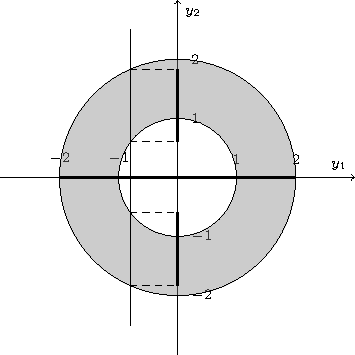
\includegraphics[width=0.8\linewidth]{figures/figure_5_5.pdf}
\caption{Sections and projections}
\label{fig:5_5}    
\end{figure}
In Fig. \ref{fig:5_5} this domain is marked with gray. The left-side line $y_1=const$  generates the section $S_1(y_1)$  as the intersection of the line with the domain $Q$, and the projection  of $S_1(y_1)$  onto the axis $y_2$  determines the projection $\Pi_2(y_1)$ . This projection and the projection $\Pi_1$  are marked with the bold lines in Fig. \ref{fig:5_5}.

These geometrical considerations allow constructing the necessary projections of the problem as 
\begin{displaymath}
\Pi_1=[-2,\:2],
\end{displaymath}
\begin{displaymath}
\Pi_2(y_1)=
  \begin{cases}
    [-\sqrt{4-y_1^2}, \sqrt{4-y_1^2}],\ y_1\in [-2,\:-1]\bigcup [1,\:2],  \\
    [-\sqrt{4-y_1^2}, -\sqrt{1-y_1^2}]\bigcup [\sqrt{1-y_1^2}, \sqrt{4-y_1^2}],y_1\in [-1,\:1].                      	
  \end{cases}
\end{displaymath}
\end{example}

However, finding all roots of a continuous function is a difficult problem, unsolvable analytically, as a rule. In this case, one can try to find these roots numerically. Let us consider, for example, typical problem (\ref{eq:5_22}). In order to find all roots of a continuous function $g(x)$ one can propose  numerical solving  the equivalent optimization problem 
\begin{displaymath}
\left|g(x)\right|\rightarrow \min,x\in [a,b],
\end{displaymath}
which roots of $g(x)$ are the global minima points in. To solve this problem, for example, the characteristical global search algorithms \cite{5_GrishaginSergeyevStrongin} providing the convergence to all global minimum points might be applied.

The case $Q=D$  when the constraint functions (\ref{eq:5_2}) are absent is an important particular case of the problem (\ref{eq:5_1})--(\ref{eq:5_3}). In this case, $G(y)\equiv 0$ in the domain $D$, and it follows from (\ref{eq:5_12}) that $G^i(u_i)\equiv 0$,$1\leq i\leq N$. Then, according to (\ref{eq:5_16}), 
\begin{displaymath}
\Pi_i(u_{i-1})=[a_i,b_i],
\end{displaymath}
where $a_i,b_i$ are constants.

The optimization domains (\ref{eq:5_2}) can generate projections $\Pi_i(u_{i-1})$  as a single interval for some special classes of the constraint functions as well. These classes are the convex functions $g_j(y),\:1\leq j\leq m$, providing the convexity of the feasible domain $Q$ and the monotonous unimodal functions \cite{5_GrishaginStrongin_EnginCybernetics}, which is more general than the convex ones.  In general case, monotonous unimodal constraints can generate non-convex domains $Q$.

In the situation of the monotonous unimodality (or of convexity as a particular case) of the constraints $g_j(y),\:1\leq j\leq m$, the one-dimensional search domains are the intervals 
\begin{displaymath}
\Pi_i(u_{i-1})=[a_i^1(u_{i-1}),b_i^1(u_{i-1})],
\end{displaymath}
the boundaries of which, however, are not constant but depend on the vector $u_{i-1}$.
\subsection {Properties of the objective functions in one-dimensional subproblems}
\label{subsec:5_2_2}

The objective function in a subproblem (\ref{eq:5_21}) is the function $\varphi^i(u_{i-1},y_i)$  with fixed $u_{i-1}$ . The character of the dependence of the function $\varphi^i$  on the variable $y_i$  is crucial while solving the subproblems (\ref{eq:5_21}).

Let us consider a class of problems, in which the function $\varphi(y)$ is separable, i.e.,
\begin{equation}
\label{eq:5_28}
\varphi(y)=\sum_{i=1}^N{\varphi_i(y_i)},
\end{equation}
and the constraints $g_j(y)$  are absent, i.e., $Q=D$.

Then, as it follows from (\ref{eq:5_18}) and (\ref{eq:5_28}), 
\begin{displaymath}
\min_{y\in Q}\varphi(y)=\sum_{i=1}^N{\min_{y_i\in [a_i,b_i]}\varphi_i(y_i)},
\end{displaymath}
i.e., to solve the multidimensional problem it is necessary to solve $N$ independent one-dimensional subproblems. For this problem class, the complexity increases linearly with increasing dimensionality. 

Now assume that the function $\varphi(y)$ satisfies the Lipschitz condition with a constant $L>0$ in the domain $Q$, i.e., for any $y',y''\in Q$
\begin{equation}
\label{eq:5_29}
\left|\varphi(y')-\varphi(y'')\right|\leq L\left\|y'-y''\right\|,
\end{equation}
where $\left\|\bullet\right\|$ denotes the Euclidean norm. The obvious question in this case is whether the functions $\varphi^i(u_i)$  satisfy the Lipschitz condition. Generally speaking, it takes place not always.

Let us consider the following example. Assume that two-dimensional objective function $\varphi(y)$  in problem (\ref{eq:5_1})--(\ref{eq:5_3}) satisfies the Lipschitz condition (\ref{eq:5_29}) and the feasible domain  
\begin{displaymath}
Q=\{y\in R^2:y_1^2+y_2^2-1\leq 0\}.
\end{displaymath}

The function $\varphi^2(y)\equiv \varphi(y)$ , obviously, is Lipschitzian with the constant $L$ for the coordinate $y_2$. However, the function $\varphi^1(y_1)$  does not satisfy the condition (\ref{eq:5_29}). As it has been shown in \cite{5_StrMonRus}, this function satisfies the generalized Lipschitz condition (H{\"o}lder condition) in the metric $\rho(y_1',y_1'')=\sqrt{\left|y_1'-y_1''\right|}$  with the constant $L_1=L(1+\sqrt{2})$ , i.e., the inequality 
\begin{displaymath}
\left|\varphi(y_1')-\varphi(y_1'')\right|\leq L_1\sqrt{\left|y_1'-y_1''\right|}.
\end{displaymath}

Sufficient conditions for the Lipschitz property (\ref{eq:5_29})  of functions $\varphi^i(u_i)$  is established by the following theorem (see \cite{5_StrMonRus}).
\begin{theorem}
\label{theor:5_1}
Assume that the function $\varphi(y)$ satisfies the Lipschitz condition (\ref{eq:5_29})  with the constant $L>0$ in a domain $Q$ from (\ref{eq:5_2}) and the boundary pairs (\ref{eq:5_25}) are the piecewise linear functions of the kind 
\begin{equation}
\label{eq:5_30}
a_i(u_{i-1})=\max_{1\leq\nu \leq p_i}\{\alpha_{i-1}^\nu u_{i-1}+A_{i-1}^\nu\},
\end{equation}
\begin{equation}
\label{eq:5_31}
b_i(u_{i-1})=\max_{1\leq\nu \leq r_i}\{\beta_{i-1}^\nu u_i+B_{i-1}^\nu\},
\end{equation}
where  $\alpha_{i-1}^\nu u_{i-1}$ and $\beta_{i-1}^\nu u_{i-1}$ are the scalar products of the vectors from $R^{i-1}$  and $A_{i-1}^\nu, B_{i-1}^\nu$ are constants. Then the functions $\varphi^i(u_i),u_i\in Q_i,$ satisfy the Lipschitz condition with the constants $L_i,1\leq i\leq N,$ 
where
\begin{displaymath}
L_N=L,\:L_i=L\sum_{j=i}^{N-1}{(1+\lambda_j)},\:1\leq i\leq N-1,
\end{displaymath}
\begin{displaymath}
\lambda_j=\max\left\{\max_{1\leq \nu\leq p_{i+1}}\left\|a_j^\nu\right\|,\max_{1\leq \nu\leq r_{i+1}}\left\|b_j^\nu\right\| \right\}.
\end{displaymath}
\end{theorem}

The proof of the theorem is given in \cite{5_StrMonRus}.

Note that the representation of the boundary pairs in the form (\ref{eq:5_30}) and (\ref{eq:5_31}) takes place if the feasible domain is a convex polyhedron. 

If the domain $Q$ is a hyperparallelepiped, all vectors $a_i^\nu,b_i^\nu$ are equal to zero. Therefore, $L_i=L,\:1\leq i\leq N$.

The main conclusion, which follows from the discussion of the Lipschitz property is that the properties of the objective functions of the one-dimensional problems depend essentially not only on the features of the initial objective function $\varphi(y)$  but also on the shape of the feasible domain $Q$.

In the simplest case, when the domain $Q$ is a hyperparallelepiped all functions $\varphi_i(u_i)$  satisfy Lipschitz condition with the same constant as the function $\varphi(y)$.

If the constraints $g_j(y)$   are piecewise linear convex functions, the Lipschitzness of the functions $\varphi_i(u_i)$  remains but Lipschitz constants for these functions increase in general that worsens the optimization properties of the one-dimensional subproblems.

Finally, the case of the nonlinear constraints can result in the loose of Lipschitzness at all.
\section{Parallel computations for the nested optimization scheme}
\label{sec:5_3}
Applying the parallel methods of the one-dimensional optimization for solving one-dimensional subproblems (\ref{eq:5_21}) in the structure of the nested scheme (\ref{eq:5_18}) enables to obtain a parallel version of the nested scheme with a high degree of variability. For example, one can vary the number of processors employed at different levels of the one-dimensional optimization (i.e., during solving the one-dimensional subproblems for different variables ), apply various parallel one-dimensional optimization methods at different levels, etc.

In order to describe the parallel nested scheme, let us introduce a vector of the parallelization degrees
\begin{equation}
\label{eq:5_32}
\pi=(\pi_1,\pi_2,\:\ldots\:,\pi_N)
\end{equation}
where $\pi_i,1\leq i\leq N$, is the number of one-dimensional subproblems at the $(i+1)$-th recursion level arising as a result of the parallel iterations at the $i$-th level of the one-dimensional optimization and being solved in parallel. The value $\pi_N$  for the coordinate $y_N$  is the number of the parallel trials during the minimization of the function $\varphi^N(y_1,\ldots y_N)\equiv  \varphi(y_1,\ldots y_N)$ with fixed values of $y_1,\ldots, y_{N-1}$, i.e., the number of the objective function values computed in parallel. 

In general, the values $\pi_i,1\leq i\leq N$, may depend on various parameters and may be changed in the course of the optimization. Here, for simplicity, we will consider the case when all components of the vector (\ref{eq:5_32}) are constant. 

The application of the one-dimensional parallel algorithms combined with scheme (\ref{eq:5_18})--(\ref{eq:5_21}) and vector (\ref{eq:5_32}) allows using up to
\begin{displaymath}
P=\prod_{i=1}^N{\pi_i}
\end{displaymath}
processors working in parallel for solving the problem (\ref{eq:5_1})--(\ref{eq:5_3}). Note, the nested scheme generates up to $P/\pi_N$  one-dimensional optimization subproblems being solved simultaneously.

Let us consider, for example, the dimensionality $N=2$. The use of a method with $\pi_1$  parallel trials at one iteration to solve the external univariate problem
\begin{displaymath}
\varphi^1(y_1)\rightarrow\min,y_1\in \Pi_1\subseteq R^1,
\end{displaymath}
generates  $\pi_1$ internal one-dimensional subproblems
\begin{displaymath}
\varphi^2(y_1,y_2)\rightarrow\min,y_2\in \Pi_2(y_1)\subseteq R^1.
\end{displaymath}
Each of these subproblems can be solved by a parallel method with  $\pi_2$  trials at iteration. It means that at the most internal level corresponding  to $i=N$  in (\ref{eq:5_21}) $P=\pi_1\pi_2$  values of the function $\varphi(y)$  are computed, i.e., one can apply $P$  processors running in parallel for computing these values. 

One of possible distributions for   $P=6$ parallel processors is presented in Fig. \ref{fig:5_6}.
\begin{figure}[t]
\centering
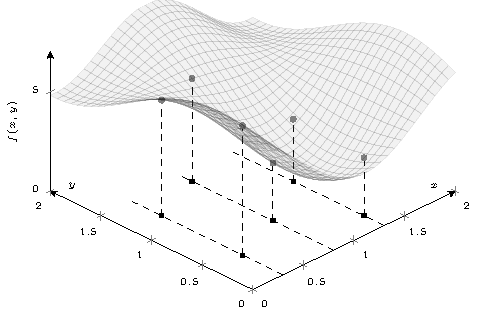
\includegraphics[width=0.8\linewidth]{figures/figure_5_6.pdf}
\caption{Distribution of processors}
\label{fig:5_6}    
\end{figure}

The nested scheme has a significant potential of the parallelization efficiency by means of the use of the asynchronism. This fact is explained by the following reasons.

Let us assume that we combine the nested scheme with a one-dimensional parallel algorithm, which the termination condition differs from realizing a fixed number of iterations in. In this case, the execution time of the trials (the computations of the minimized function) in a parallel iteration at the $i$-th level of the recursion ($1\leq i\leq N-1$)  are different necessarily even if the computation time of the objective function $\varphi(y)$  is independent on the arguments. Remind that the evaluation of the objective function at all levels except the last one consists in solving of a new optimization subproblem.

Assume that the synchronous scheme of the parallel iterations of the one-dimensional optimization algorithm is applied at the $i$-th level of recursion, when the iteration is considered to be complete after execution of all $\pi_i$   trials only. In this case, at least 
\begin{displaymath}
\prod_{j=i+1}^N{\pi_j}
\end{displaymath}
processors, which have already completed solving their subproblems stay idle until the rest subproblems of the $i$-th level are completed. This means that for increasing the productivity of the solving process in the nested scheme it is necessary to use the asynchronous parallel global optimization algorithms, in which the computational resources are used immediately after they become free.

\paragraph{Numerical experiments}

In order to illustrate the theoretical statements, the results of the numerical solving of different multidimensional multiextremal problems are presented below. Three methods which realize multidimensional optimization using the nested scheme (\ref{eq:5_18})--(\ref{eq:5_21}) with combination of information univariate algorithms are considered:
\begin{description} [1)]
\item [1)] {AGSM– algorithm of global search which solves the one-dimensional subproblems inside of the nested scheme by the sequential core information global search algorithm \cite{5_StrSergMon2000};}
\item [2)] {PSIM – parallel synchronous information algorithm. It uses the algorithm AGSIP \cite{5_GriKvaMukhStr} for solving the one-dimensional subproblems (\ref{eq:5_21});}
\item [3)] {AIPM – asynchronous multidimensional information parallel algorithm proposed in \cite{5_SergGriJCAA}.}
\end{description}

The following assumptions are introduced for the first two series of experiments.
\begin{description} [i)]
\item [i)] {The times required for computation of the objective function values are the same for all feasible points. This time can be used as a “unit” time or a “quantum” of time  in the search process. Note, that this assumption is the worst case for the asynchronous method since it is more suitable for the synchronous parallelization.}
\item [ii)] {The time for computation of the objective function value is much greater than the one spent for the implementation of the computational operations of the algorithmic scheme.}
\end{description}

This approach allows abstracting from the architecture of the parallel computational system, on which the experiments are carried out and estimate the «pure» efficiency of the algorithm decision rules. 

Let us denote the time of solving the multidimensional problem (measured in the computational quanta) using the nested reduction scheme with application of the asynchronous algorithm AIPM and the parallelization vector (\ref{eq:5_32}) as $T_A(\pi)=T_A(\pi_1,\pi_2,\ldots,\pi_N)$ , the one with the use of the synchronous algorithm PSIM  (in the analogous conditions) as $T_S(\pi)=T_S(\pi_1,\pi_2,\ldots,\pi_N)$ , and the one with the use of the sequential method AGSM as $T_1=T_S(1,1,\ldots,1)=T_A(1,1,\ldots,1)$ . The last time is simply equal to the number of the computed values of the function $\varphi(y)$.

Furthermore, the numbers of trials performed by the asynchronous method and by the synchronous one will be denoted as $K_A$  and $K_S$, respectively. Using the introduced values, one can define the corresponding time speed-ups achieved owing to the parallelism.

$u_S(\pi)=T_1/T_S(\pi)$ is the speed up of the synchronous algorithm.

$u_A(\pi)=T_1/T_A(\pi)$ is the speed up of the asynchronous algorithm.

As a measure for the comparison of the relative efficiency of the synchronism and the asynchronism the coefficient $u(\pi)=u_A(\pi)/u_S(\pi)$ is introduced.

Note that because of Assumption (i) in the case $\pi=(1,1,\ldots,1,\pi_N)$  we have $u_A(\pi)=u_S(\pi)$ and $u(\pi)=1$.

In the first experiment, the maximization of 100 two-dimensional functions from the class (\ref{eq:5_GriFun}) has been carried out. All experiments were carried out with the precision in the termination criterion $\epsilon=0.01$  and with the reliability parameter $r=2$  for solving all one-dimensional subproblems (\ref{eq:5_21}). All one-dimensional searches have been started from the same starting points {0.2, 0.3, 0.7, 0.8}.

For the method AGSM, which is a pure sequential one, the average number of trials determined as a result of the maximization of 100 functions of the class (\ref{eq:5_GriFun}) was found to be  $T_1= 415.08$. This value can be considered as a measure for the average search time. 

The results for the parallel methods are presented in Table \ref{tab:5_1}.

\begin{table}
\caption{Comparison of the parallel algorithms on the two-dimensional test class}
\label {tab:5_1}
\begin{center}
\begin{tabular}{|c|r|r|r|r|r|}
\hline
$q$ & (2,1) & (2,2) & (2,3) & (2,4) & (2,5)   \\
\hline
$\ \ $$K_A\ \ $  &  $\ \ \ $409.46 & $\ \ \ $397.96 & $\ \ \ $419.41 & $\ \ \ $456.00 & $\ \ \ $510.60  \\
\hline
$K_S$  & 413.89 & 409.24 & 424.08 & 458.60 & 514.20  \\
\hline
$T_A$  & 204.73 &  99.49 &  69.90 &  57.00 &  51.06  \\
\hline
$T_S$  & 234.52 & 114.63 &  77.79 &  62.46 &  56.89  \\
\hline
$u_A$  &   2.03 &   4.17 &   5.94 &   7.28 &   8.13  \\  
\hline
$u_S$  &   1.77 &   3.62 &   5.34 &   6.64 &   7.30  \\
\hline
$u$    &   1,15 &   1,15 &   1,11 &   1,10 &   1,23  \\
\hline
\hline
$q$ & (3,1) & (3,2) & (3,3) & (3,4) & (3,5)   \\
\hline
$K_A$  & 427.23 & 429.18 & 432.90 & 472.20 & 529.95  \\
\hline
$K_S$  & 432.40 & 426.16 & 433,83 & 469.44 & 527.90  \\
\hline
$T_A$  & 123.41 &  71.53 &  48.10 &  39.35 &  35.33  \\
\hline
$T_S$  & 174.38 &  84.90 &  55.95 &  44.63 &  40.62  \\
\hline
$u_A$  &   2.91 &   5.80 &   8.63 &  10.55 &  11.75  \\
\hline
$u_S$  &   2.38 &   4.89 &   7.42 &   9.30 &  10.22  \\
\hline
$u$    &   1.22 &   1.19 &   1.16 &   1.13 &   1.15  \\
\hline
\hline
$q$ & (4,1) & (4,2) & (4,3) & (4,4) & (4,5)   \\
\hline
$K_A$  & 459.88 & 447.12 & 469.32 & 494.40 & 565.20  \\
\hline
$K_S$  & 458.09 & 459.38 & 466.44 & 502.08 & 570.70  \\
\hline
$T_A$  & 114.97 &  55.89 &  39.11 &  30.90 &  28.26  \\
\hline
$T_S$  & 144.45 &  71.38 &  46.58 &  36.92 &  33.69  \\
\hline
$u_A$  &   3.61 &   7.43 &  10.61 &  13.43 &  14.69  \\
\hline
$u_S$  &   2.87 &   5.82 &   8.91 &  11.24 &  12.32  \\
\hline
$u$    &   1.26 &   1.28 &   1.19 &   1.19 &   1.19  \\
\hline
\end{tabular}
\end{center}
\end{table}

The next series of the experiments consists in the minimization of the multidimensional function \cite{5_LucidiPiccioni}
\begin{equation}
\label{eq:5_33}
\varphi(y)=\frac{\pi}{N}\left\{10\sin^2(\pi y_1)+(y_N-1)^2+\sum_{i=1}^{N-1}{[(y_i-1)^2)(1+10\sin^2(\pi y_{i+1})]}    \right\}
\end{equation}
where $-2\leq y_i\leq 4,\;1\leq i\leq N$, for the dimensions $N=$ 3, 4, and 5. The precision $\epsilon=0.12$ and the reliability parameter $r = 2$ were used in all the experiments. At the initial search steps the first four trials were conducted at the points {-1.2, -0.5, 0.0, 2.2} in all one-dimensional subproblems (\ref{eq:5_21}). The results of the computations for the parallel algorithms are presented in Table \ref{tab:5_2}.
\begin{table}
\caption{Comparison of the parallel algorithms for the functions (\ref{eq:5_33}) of various dimensions}
\label {tab:5_2}
\begin{center}
\begin{tabular}{|c|c|c|c|c|c|}
\hline
\multirow{8}{*}{$N=3$} & $q$ & (1,1,1) & (2,2,2) & (3,3,3) & (4,4,4) \\
\cline{2-6}
		& $K_A$ &  7 791  &  7 056  &  7 884  &  10 368   \\
\cline{2-6}
		& $K_S$ &  7 791  &  6 772  &  7 548  &  10 836   \\
\cline{2-6}
		& $T_A$ &  7 791  &   882  &   292  &    162   \\	
\cline{2-6}
		& $T_S$ &  7 791  &  1 013  &   390  &    216   \\		
\cline{2-6}
		& $u_A$ &  1.00  &  8.83  & 26.68  &  48.09   \\
\cline{2-6}
		& $u_S$ &  1.00  &  7.69  & 19.98  &  36.07   \\
\cline{2-6}
		& $u$   &  1.00  &  1.15  &  1.34  &   1.33   \\
\hline
\hline
\multirow{8}{*}{$N=4$} & $q$ & (1,1,1,1) & (2,2,2,2) & (3,3,3,3) & (4,4,4,4) \\  
\cline{2-6}
		& $K_A$ &  155 694  &  136 576  &  165 807  &  201 216   \\
\cline{2-6}
		& $K_S$ &  155 694  &  130 168  &  152 895  &  232 682   \\
\cline{2-6}
		& $T_A$ &  155 694  &  8 536  &   2 047  &   786   \\	
\cline{2-6}
		& $T_S$ &  155 694  & 10 658  &  3 062  &    1 296   \\		
\cline{2-6}
		& $u_A$ &  1.00  & 18.24  & 76.06  & 198.08   \\
\cline{2-6}
		& $u_S$ &  1.00  & 14.61  & 50.85  & 120.13   \\
\cline{2-6}
		& $u$   &  1.00  &  1.25  &  1.50  &   1.65   \\
\hline
\hline
\multirow{8}{*}{$N=5$} & $q$ & (1,1,1,1,1) & (2,2,2,2,2) & (3,3,3,3,3) & (4,4,4,4,4) \\  
\cline{2-6}
		& $K_A$ &  3111771  &  2635872  &  3258144  &  4786176   \\
\cline{2-6}
		& $K_S$ &  3111771  &  2502128  &  3097143  &  4996416   \\
\cline{2-6}
		& $T_A$ &  3111771  &  82371  &   13408  &   4674   \\	
\cline{2-6}
		& $T_S$ &  3111771  & 112485  &  24119  &    7776   \\		
\cline{2-6}
		& $u_A$ &  1.00  & 37.78  & 232.08  & 665.76   \\
\cline{2-6}
		& $u_S$ &  1.00  & 27.66  & 129.02  & 400.18   \\
\cline{2-6}
		& $u$   &  1.00  &  1.36  &  1.80  &   1.67   \\
\hline
\end{tabular}
\end{center}
\end{table}

In the next series of experiments, the function computation time was assumed to depend on the trial point. Problem (\ref{eq:5_33}) was considered for  $N=3$; the precision of the method $\epsilon=0.01$ and the reliability parameter $r=2$ were taken. In all one-dimensional subproblems (\ref{eq:5_21}) the first four trials were conducted at the points {-1.2, -0.5, 0.0, 2.2}. The two kinds of the dependencies $t(y)$ of the function value computation time per one trial point were used. In experiment A
\begin{displaymath}
t_1(y)=\left\lfloor 999\frac{\varphi(y)-\varphi_{min}}{\varphi_{min}-\varphi_{max}}\right\rfloor,
\end{displaymath}
where $\left\lfloor x\right\rfloor$  is the integer part of $x$, $\varphi_{min}=0$, $\varphi_{max}=185$, and in experiment B
\begin{displaymath}
t_2(y)=1000-t_1(y)
\end{displaymath}
were used.

Table \ref{tab:5_3} contains the results of the experiments A and B.
\begin{table}
\caption{Comparison of parallel algorithms in the case of variable time of trial execution}
\label {tab:5_3}
\begin{center}
\begin{tabular}{|c|c|c|c|c|}
\hline
 & \multicolumn{2}{c|}{Experiment A} & \multicolumn{2}{c|}{Experiment B} \\
\hline
$q$ & (2,2,2) & (3,3,3) & (2,2,2) & (3,3,3)    \\
\hline
$K_A$ & 106 802 & 117 270 & 105 599 & 111 774 \\
\hline
$K_S$ & 101 510 & 103 671 & 101 510 & 103 671 \\
\hline
$T_A$ & 738 361 & 221 739 & 11 900 017 & 3 629 895 \\
\hline
$T_S$ & 1 527 229 & 791 559 & 16 943 876 & 5 769 930 \\
\hline
$u$   & 2.07  &  3.57  &  1.42  &  1.59  \\
\hline
\end{tabular}
\end{center}
\end{table}

It results from Table \ref{tab:5_3} that both the parallel methods make a small number of redundant trials only, and the asynchronous algorithm is faster than the synchronous one.

Now let us consider a parallel characteristical algorithm \cite{5_GrishaginSergeyevStrongin}. It is possible construct its implementation for the synchronous and asynchronous cases and compare the speed-ups of these versions as a measure of parallelization efficiency. This approach allows estimating the potential of various parallelization schemes of the algorithm decision rules. In the framework of this approach, the experiments were carried out for core information global search algorithm \cite{5_StrSergMon2000} for the  class of functions of various dimensionality. The average values of $u_S(\pi)$ and $u_A(\pi)$ obtained by the optimization of 100 multiextremal two-dimensional functions selected randomly from the test class (\ref{eq:5_GriFun}) are presented in Fig. \ref{fig:5_7}. 
\begin{figure}[t]
\centering
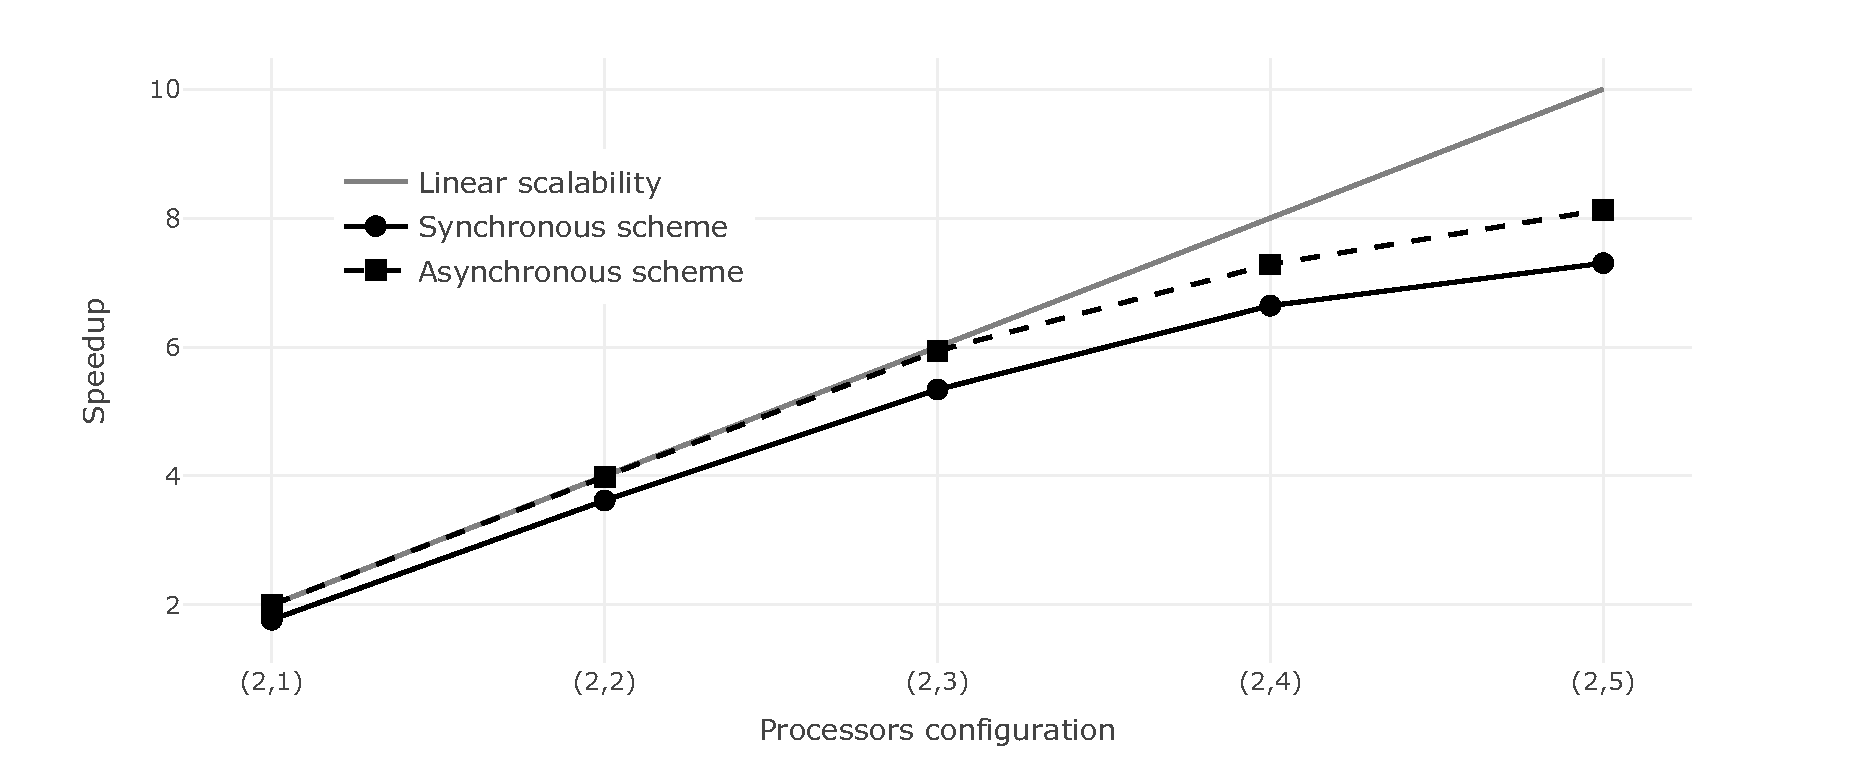
\includegraphics[width=0.8\linewidth]{figures/figure_5_7.pdf}
\caption{Comparative speed-ups of the synchronous scheme and of the asynchronous one on the two-dimensional test function class}
\label{fig:5_7}    
\end{figure}
The function plots demonstrate the dependencies of the speed up (the ordinate axis) on parallelization vector (\ref{eq:5_32}), the variants of which are shown on the abscissa axis. The upper plot corresponds to the «ideal» speed up. The middle and the lower plots reflect the speed-ups of the asynchronous scheme and of the synchronous one, respectively. 

An analogous graph for the case of the optimization of the multiextremal five-dimensional function
\begin{displaymath}
\varphi(y)=\frac{\pi}{5}\left(\sin^2(\pi y_1)+5(y_5-1)^2+\sum_{i=1}^4{[(y_i-1)^2)(1+10\sin^2(\pi y_{i+1})]}    \right)
\end{displaymath}
is presented in Fig. \ref{fig:5_8}. For the one-dimensional optimization the parallel version of the broken lines method (see \cite{5_GriKvaMukhStr, 5_Piyavskij}) with the adaptive estimate of Lipschitz constant was used.
\begin{figure}[t]
\centering
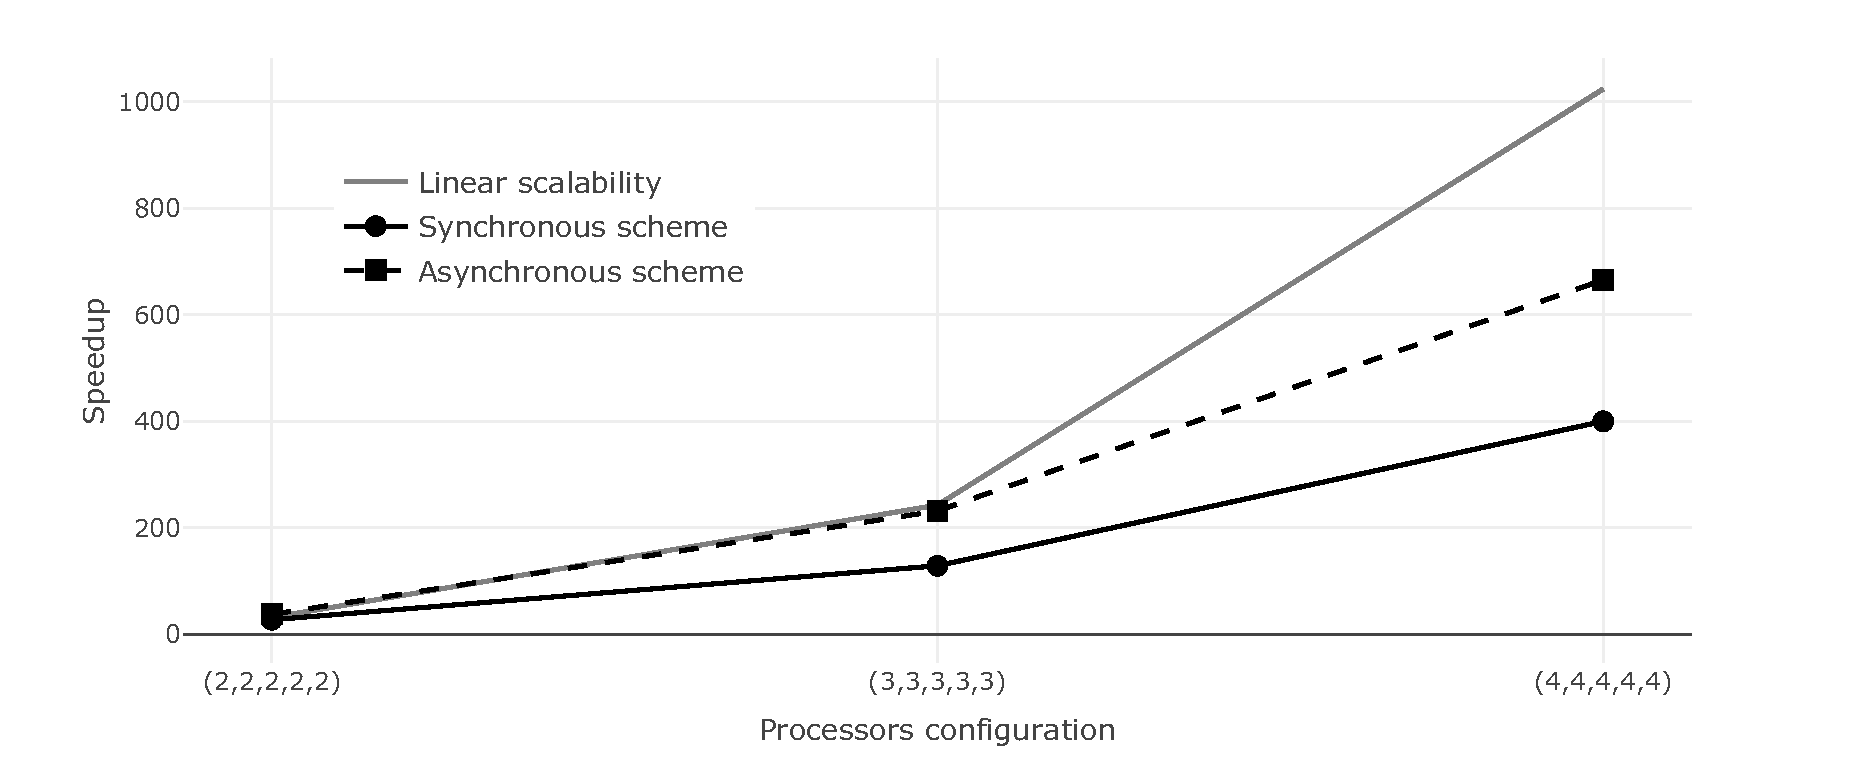
\includegraphics[width=0.8\linewidth]{figures/figure_5_8.pdf}
\caption{Speed-ups of the synchronous and asynchronous broken lines method}
\label{fig:5_8}    
\end{figure}

As in the previous case, the upper plot corresponds to the «ideal» speed up. The middle and lower plots reflect the speed-up of the asynchronous scheme and of the synchronous one, respectively. 
\section{Adaptive nested scheme of dimensionality reduction}
\label{sec:5_4}
\subsection {General description}
\label{subsec:5_4_1}
The univariate subproblems of the family (\ref{eq:5_21}) are generated recursively and it is possible to describe their connections using a hierarchical structure “tree” in which  the root is the subproblem (\ref{eq:5_19}) and the leaves are the subproblems (\ref{eq:5_20}). An example of the full subproblems’  tree (obtained after completion of solving all the family (\ref{eq:5_21})) for the dimension $N=3$  is shown in Fig. \ref{fig:5_9}.
\begin{figure}[ht]
\centering
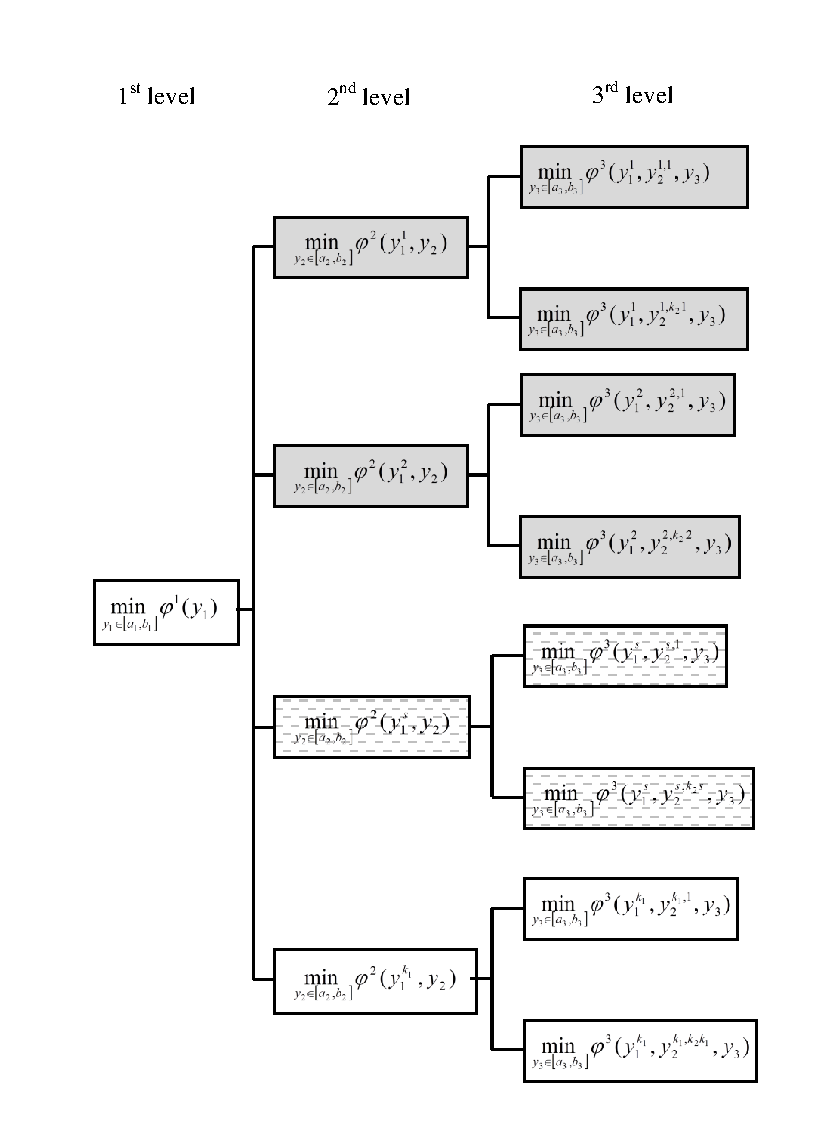
\includegraphics[width=1.0\linewidth]{figures/figure_5_9.pdf}
\caption{Tree of subproblems in the nested optimization scheme}
\label{fig:5_9}    
\end{figure}

In the classical implementation of the nested scheme there are some important features. Namely, execution of any trial in a subproblem at the level $i<N$ generates a sub-tree of the general tree (the execution of a trial in a subproblem at the level $i=N$ consists in computation of the objective function $\varphi(y)$ from (\ref{eq:5_1})). For example, in the root subproblem (\ref{eq:5_19})  the trial at the point $y_1^s$  requires solving univariate subproblems of the sub-tree marked in Fig.\ref{fig:5_9} with the background as the dashed lines. Moreover, until the subproblems of this sub-tree will be completely solved no new trial can be initiated in the root subtask. As a consequence, while solving the subproblems belonging to the dashed sub-tree the subproblems corresponding to the other sub-trees either have been solved already (they are marked in Fig \ref{fig:5_9} with grey) or will be solved later (marked with no background).

As it follows from the presented structure the subproblems at the same level are solved independently and the search information obtained in a subproblem is not used in the other subproblems at this level (and, of course, in all sub-trees generated them).  Such loss of information leads to increasing the number of trials and slows up the optimization process. 

To overcome this drawback in the paper \cite{5_GerGriGer} a new version of the nested optimization scheme in which the other way of solving the univariate subproblems has been proposed. In this version called \textit{adaptive nested optimization scheme} instead of the strictly subordinated order of solving the univariate subproblems the principle of simultaneous consideration of all subproblems arising dynamically is used. The adaptive scheme does not require to solve each  one-dimensional subproblem  up to the end and all the generated subproblems participate in the multidimensional optimization at any iteration of its realization. The main principle of such realization is close to the idea of characteristical algorithms  \cite{5_GriKvaMukhStr, 5_GrishaginSergeyevStrongin}. Namely, to each subproblem a numerical value called its characteristic is assigned and the multidimensional iteration consists in the choice of the subproblem with maximal characteristic and performing a new trial in this subtask. If the characteristics are assigned in such a way that they take into account the values of functions minimized in subproblems following the principle 'low values influence increasing the characteristic' then the subproblems with lower values will be chosen more often than the subproblems with the higher ones and computational resources will not be spent for solving the latters unlike the classical nested scheme where these subproblems have to be solved completely. 

The detailed algorithmic implementation of the adaptive nested scheme can be found in \cite{5_GerGriGer}. Here we give a description of this scheme in a general form.

\textbf{Start stage.}

Create in some way an initial set $S$  of subproblems (\ref{eq:5_21}) including a few subproblems at each level of recursion.
\begin{description} [\textbf{Step G1.}]
\item [\textbf{Step G1.}] {Juxtapose to each subproblem from the set $S$ a numerical value called \textit{characteristic} of this problem.}
\item [\textbf{Step G2.}] {Choose the subproblem with the greatest characteristic (the currently best subproblem).}
\item [\textbf{Step G3.}]{Compute a new trial point in the chosen subproblem.}
\item [\textbf{Step G4.}]{Build the sub-tree of subtasks generated by this trial point in accordance with the nested scheme  (\ref{eq:5_18})--(\ref{eq:5_21}) and add new subproblems to the set $S$.}
\item [\textbf{Step G5.}]{If the termination  criterion is fulfilled in the root subproblem (\ref{eq:5_19}) stop the search and take as a result of optimization the least computed value of the objective function $\varphi(y)$ and its coordinates as the global minimizer. Otherwise, go to \textbf{Step G1}.}
\end{description}

The crucial question arising in the general scheme is how to choose characteristics of the subproblems.  A possible way can be suggested if for solving the subproblems (\ref{eq:5_21}) a one-dimensional characteristical algorithm is used. In this case as the characteristic of the subtask one can take the best interval characteristic of this method. Moreover, as a stopping criterion of the multidimensional search the termination criterion  in the root problem (\ref{eq:5_19}) can be taken, i.e., the multidimensional optimization is stopped when the interval with the maximal characteristic in the subproblem (\ref{eq:5_19}) becomes less than predefined accuracy. 

For realization of this idea the core information  global search algorithm  (see \cite{5_GriKvaMukhStr, 5_StrSergMon2000}) can be taken. Theorem ~\ref{theor:5_2} gives the theoretical substantiation of convergence to global minimum for the adaptive nested scheme combined with AGS for solving internal univariate subproblems (\ref{eq:5_21}).

Before formulating the theorem let us introduce a few notations. First of all, it is necessary to pay attention that during realization of the adaptive scheme the values of objective functions   in subproblems (\ref{eq:5_21}) for $1\leq i\leq N-1$   are evaluated approximately, as for obtaining the exact value $\varphi^i(u_{i-1},\tilde{y_i})$ at a 
point  $\tilde{y_i}$  it is required to minimize exactly the function $\varphi^{i+1}(u_{i-1},\tilde{y_i},y_{i+1})$  
at the next level of recursion. So, instead of exact values  $\varphi^i(u_{i-1},y_i^q),\:1\leq q\leq k_i$,   at trial 
points $y_i^1,\ldots,y_i^{k+i}$  we have the values  $\psi^i(u_{i-1},y_i^q),\:1\leq q\leq k_i$,  such that 
\begin{equation}
\label{eq:5_34}
\left|\varphi^i(u_{i-1},y_i^q)-\psi^i(u_{i-1},y_i^q)\right|\leq \gamma_q^i,1\leq q\leq k_i,
\end{equation}
where $\gamma_q^i$ can be interpreted as errors of evaluations for the exact values $\varphi^i(u_{i-1},y_i^q)$, $1\leq q\leq k_i$. As a consequence, after termination of the multidimensional optimization instead of global minimum $\varphi^*$  of the function (\ref{eq:5_1})  there is an approximate estimate $\psi^*$ of it. In this regard the question on the proximity of values $\varphi^*$ and  $\psi^*$ is very important. The answer gives the following theorem (see \cite{5_GerGriGer}).
\begin{theorem}
\label{theor:5_2}
Let the problem (\ref{eq:5_1})--(\ref{eq:5_3}) be considered without functional constraints (\ref{eq:5_2}), i.e., the admissible domain $Q$ coincides with the hyperparallelepiped $D$, and in the adaptive scheme  the information global search algorithm \cite{5_GriKvaMukhStr, 5_StrSergMon2000} be applied for one-dimensional optimization (\ref{eq:5_21}). If
\begin{enumerate}
\item {the objective function $\varphi(y)$  of the problem (\ref{eq:5_1}) satisfies in the domain $D$  the Lipschitz condition (\ref{eq:5_29}) with a finite constant $L>0$;}
\item {during solving the subproblems (\ref{eq:5_21}) the parameter $m$ of the algorithm satisfies the inequality $m>2L$;}
\item {while solving the root problem (\ref{eq:5_19}) the termination criterion is absent;}
\item {for any function $\varphi^i(u_{i-1},y_i)$  of the family (\ref{eq:5_21}) the conditions 
\begin{equation}
\label{eq:5_35}
\gamma_{\tau-1}^i+\gamma_\tau^i\leq 2\varphi(y^*)+L(y_i^\tau-y_i^{\tau-1})--(\varphi(u_{i-1},y_i^{\tau-1}+\varphi(u_{i-1},y_i^\tau)
\end{equation}
hold for the computational errors $\gamma_{\tau-1}^i,\gamma_\tau^i$  of trials at the adjacent points $ y_i^{\tau-1},y_i^\tau$ such that
\begin{displaymath}
y_i^{\tau-1}\leq y_i^*\leq y_i^\tau,
\end{displaymath}
where $y^*=(y_1^*,\ldots,y_N^*)$  is the global minimizer of the problem (\ref{eq:5_1})--(\ref{eq:5_3}),}
\end{enumerate}
then the sequence of multidimensional trials generated by the adaptive scheme converges to the global minimizer $y^*$ .
\end{theorem}

This theorem provides sufficient conditions of convergence to global minimum for the adaptive scheme in the combination with the core information global search algorithm. The proof of the theorem can be found in \cite{5_GerGriGer}. Analogous theorem for the adaptive nested scheme with combination of the univariate broken lines method \cite{5_Piyavskij} has been given in \cite{5_GriIsrSergAMC}.
\subsection {Numerical experiments}
\label{subsec:5_4_2}
To demonstrate the efficiency of the adaptive nested scheme let us consider a function from the 2-dimensional test class (\ref{eq:5_GriFun}). In Fig.~\ref{fig:5_10} the level curves of this function and distribution of trials (marked by points) are presented. The left panel corresponds to the adaptive scheme and the right panel to the classical one. For optimization of the function these schemes are used in combination with the core information global search algorithm \cite{5_GriKvaMukhStr, 5_StrSergMon2000} for solving the univariate subproblems (\ref{eq:5_21}). In both the cases the algorithm parameter $r=3$  and the search accuracy $\epsilon=0.01$ in termination criterion were used.
\begin{figure}[ht]
\centering
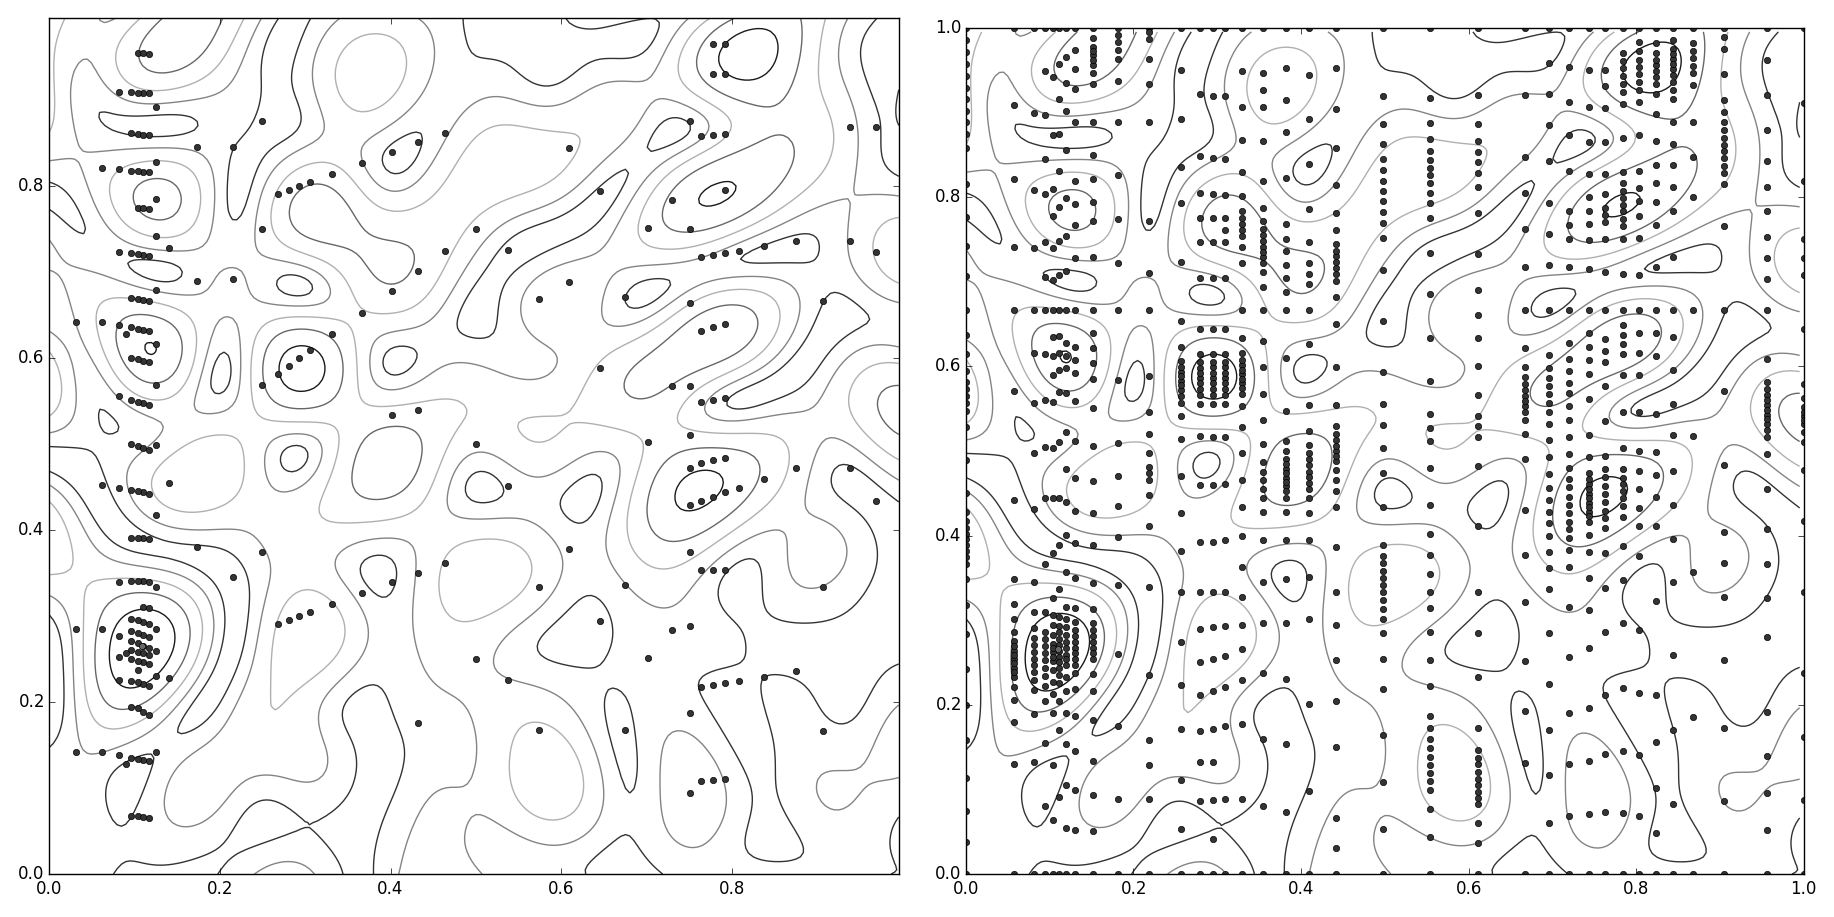
\includegraphics[width=1.0\linewidth]{figures/figure_5_10.png}
\caption{Trials distribution of the adaptive scheme (the left panel) and of the classical one (the right panel).}
\label{fig:5_10}    
\end{figure}

Both the schemes have provided the required accuracy of the problem solution. However, the adaptive scheme has spent significantly less trials, namely, the classical scheme evaluated the objective function 1139 times while the adaptive version carried out 257 trials only.

Another experiment was executed \cite{5_GriIsrSergAMC} on the set of 100 three-dimensional functions belonging to the well-known test class GKLS \cite{5_GavianoKvasovLeraSergeyev}. The GKLS parameters of the test functions were as follows:
\begin{itemize}
\item {10 local minima;}
\item {standard function value -1.0 at the  global minimizer;}
\item{distance 0.9 from the global minimizer to the vertex of the paraboloid;}
\item{radius 0.12 of the attraction region of the global minimizer.}
\end{itemize}

The following algorithms were compared by means of the method of operational characteristics: the adaptive nested scheme (AGS-A) and the classical nested scheme (AGS-C) with the core information global search algorithm inside of both the schemes, and the very popular method DIRECT \cite{5_Jones, 5_JonesPerttunenStuckman} as an example of global optimization methods of different nature. 
Operational characteristics (see \cite{5_GrishaginOperChar, 5_GriKvaMukhStr, 5_StrSergMon2000}) of the methods compared are presented in Fig. ~\ref{fig:5_11}.
\begin{figure}[ht]
\centering
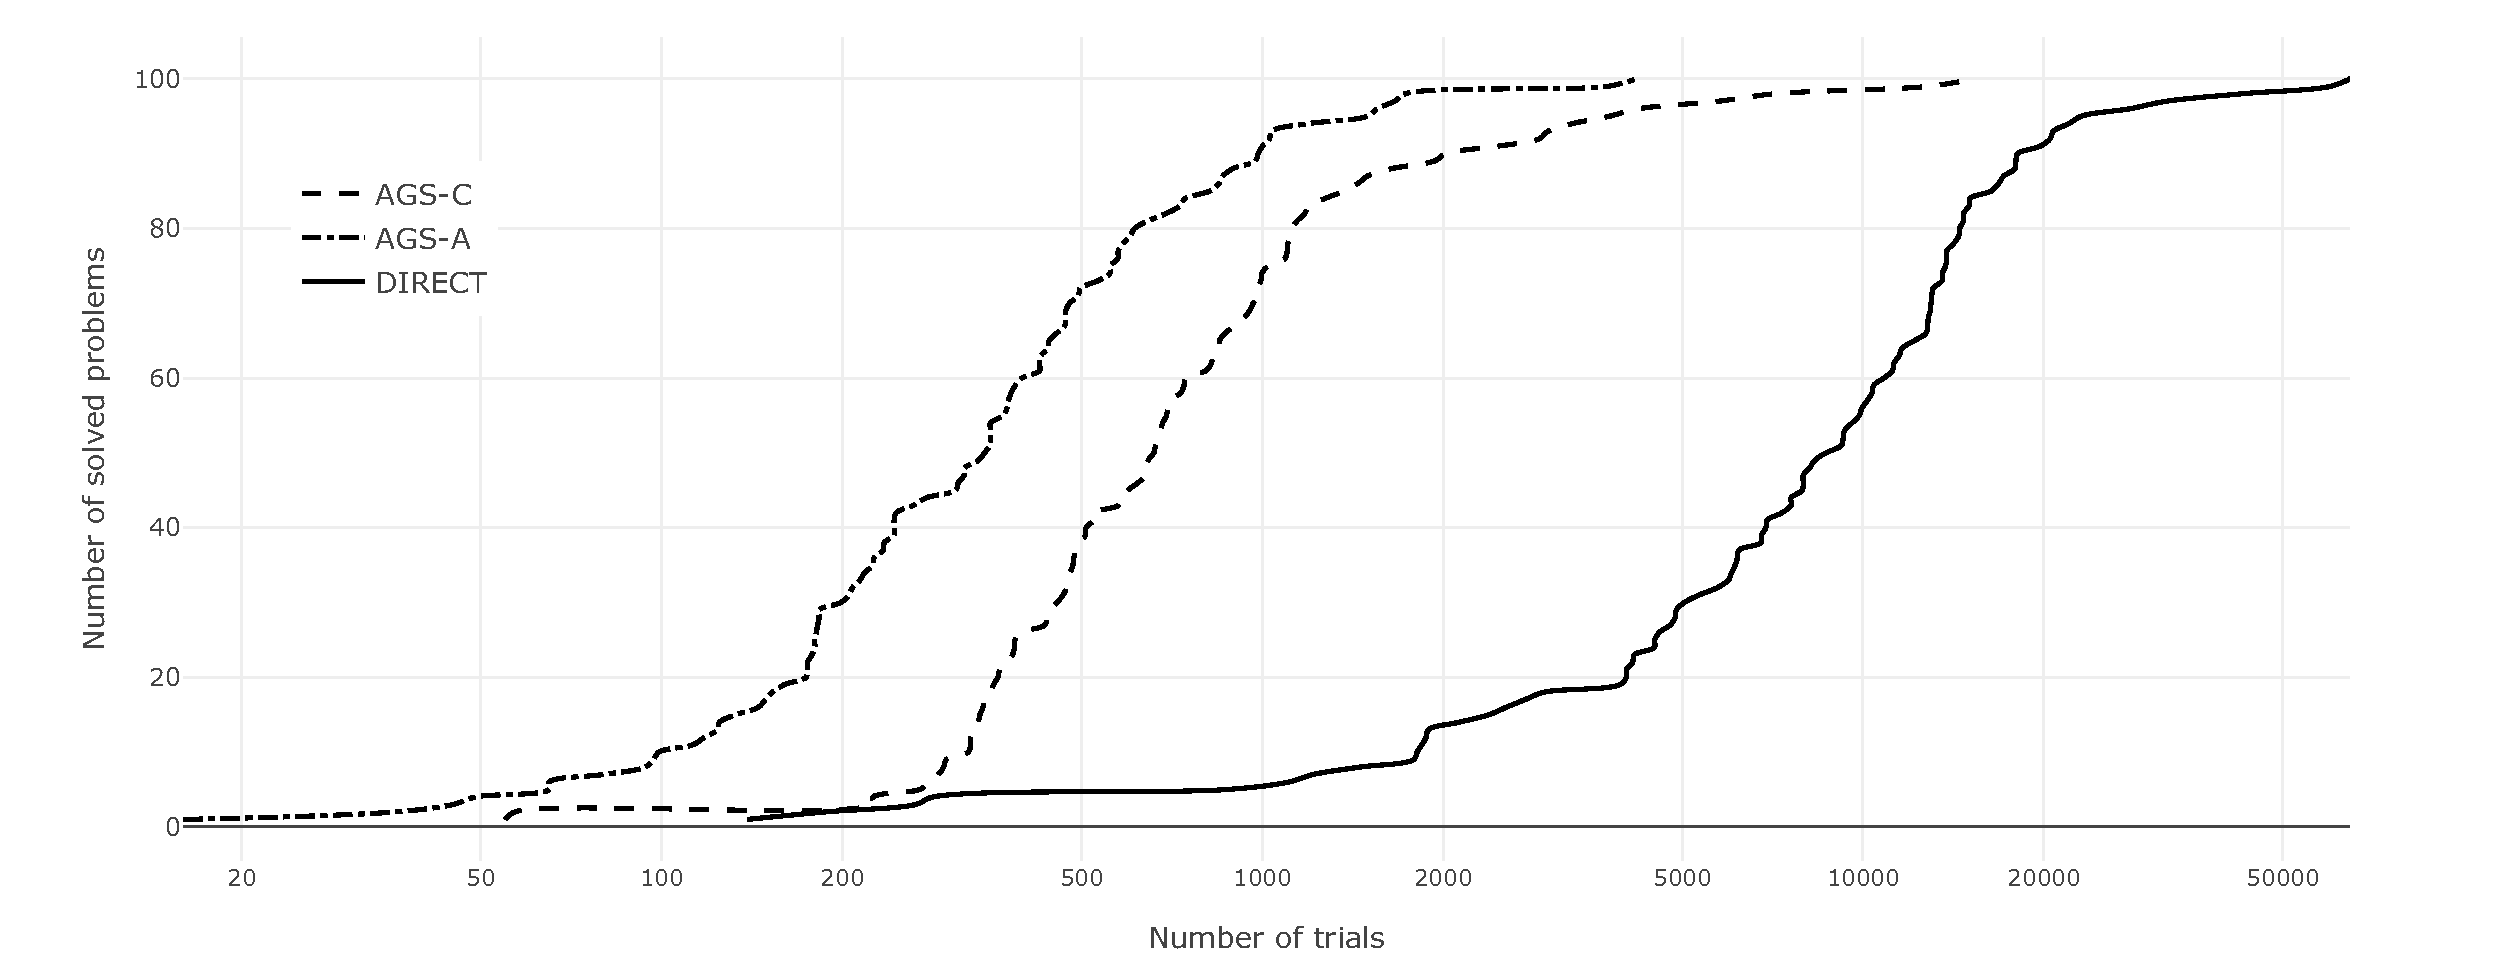
\includegraphics[width=1.0\linewidth]{figures/figure_5_11.pdf}
\caption{Operational characteristics of the nested optimization schemes and the method DIRECT.}
\label{fig:5_11}    
\end{figure}

As it follows from the presented examples and it is confirmed in other researches (see, for instance, \cite{5_GerGriGer, 5_GriIsrSergAIP, 5_GriIsrSergAMC}) the adaptive nested scheme improves significantly the results of optimization compared with its classical prototype. 

\subsection{Parallel adaptive scheme of nested optimization}
\label{subsec:5_4_3}
As well as the classical nested scheme, the adaptive one can be parallelized. The idea of parallelizing is similar to the approach applied in the parallel characteristical algorithms \cite{5_GrishaginSergeyevStrongin}. Namely, when in a multiprocessor environment there are $p>1$ free processors, in the decision rule of the general stage for the choice of the subproblems for further solving one can take $p$ subproblems with the best characteristics. For more details, let us reformulate for the parallel case the general description of the sequential adaptive scheme modifying Steps G2-G4.

\paragraph{\textbf{General iteration of synchronous adaptive scheme}}
\begin{description} [\textbf{Step G1.}]
\item [\textbf{Step G1.}] {Juxtapose to each subproblem from the set $S$  a numerical value called characteristic of this problem.}
\item [\textbf{Step G2.}] {Choose $p$ subproblems with the greatest characteristics.}
\item [\textbf{Step G3.}]{Compute new trial points in the chosen subproblems and assign to each point one processor from the pool of free processors.}
\item [\textbf{Step G4.}]{Build in parallel the sub-trees of subtasks generated by these trial points in accordance with the nested scheme (\ref{eq:5_18})--(\ref{eq:5_21}) and add new subproblems of these sub-trees to the set $S$.}
\item [\textbf{Step G5.}]{If the termination  criterion is fulfilled in the root subproblem (\ref{eq:5_19}) stop the search and take as a result of optimization the least computed value of the objective function $\varphi(y)$ and its coordinates as the global minimizer. Otherwise, go to  \textbf{Step G1}.}
\end{description}

In this description, the computational parallel procedure is implicitly supposed to be synchronous since a new iteration G1-G5 can start after completion of  building all the sub-trees at Step G4 only.  Obviously, the times of building those can differ significantly. As a result, the processors completing computations wait until the slowest processor finishes and the new iteration of the general computational procedure can go on thereafter only. To avoid standing idle one can to use an asynchronous version of the parallel adaptive scheme presented below.

\paragraph{\textbf{General iteration of asynchronous adaptive scheme}}
\begin{description} [\textbf{Step G1.}]
\item [\textbf{Step G1.}] {If there are $1\leq\pi\leq p$ free processors go to \textbf{Step G2}. Otherwise, if there are no accessible processors, wait until $\pi,\:1\leq\pi\leq p$ processors have completed computations. After that add to the set $S$ new subproblems generated by processors having finished and go to the next \textbf{Step G2}.}
\item [\textbf{Step G2.}] {If the termination criterion is fulfilled in the root subproblem (\ref{eq:5_19}) stop the search and take as a result of optimization the least computed value of the objective function $\varphi(y)$ and its coordinates as the global minimizer. Otherwise, go to \textbf{Step G3}.}
\item [\textbf{Step G3.}]{Juxtapose to each subproblem from the set $S$ a numerical value called characteristic of this problem and choose $\pi$  subproblems with the greatest characteristic (the currently best subproblems).}
\item [\textbf{Step G4.}]{Compute new trial points in the chosen subproblems and assign to each point one processor from the pool of free processors.}
\item [\textbf{Step G5.}]{Begin solving subproblems generated by these trial points in accordance with the nested scheme  (\ref{eq:5_18})--(\ref{eq:5_21}) and go to \textbf{Step G1}.}
\end{description}

The description of general computational procedure for both the synchronous and asynchronous adaptive schemes is just a “skeleton” which requires many important details for a real implementation. For example, how to realize the stage of initialization, how to keep in memory the set of subproblems $S$, or how to organize the information exchange between processors?  It should be noted as well that in adaptive scheme the subproblems of a sub-tree do not required to be solved up to the end, i.e., up to fulfillment of termination criterion in univariate algorithm solving them as it is done in the classical nested scheme. In this situation the following question arises: how to stop the one-dimensional search during solving subproblems (\ref{eq:5_21})?  Moreover, the implementation of the adaptive scheme depends in many ways on the univariate methods use inside it. These and other peculiarities of possible implementation indicate a considerable variability of the adaptive scheme and require further investigations of increasing efficiency by means of new combinations of the general scheme with different univariate methods.

In conclusion some comparative results for the sequential and asynchronous versions of the adaptive scheme are presented. For the experiment the test class GKLS \cite{5_GavianoKvasovLeraSergeyev} was taken and test sets of functions for dimensions 7 and 8 were used. For univariate optimization inside the multidimensional search the information statistical method AGS was applied in all the cases. Computations were executed on a cluster consisting of 4 nodes with 4 processors Intel® Xeon® E7-8890 v4 and each processor contained 24 cores. Parallelization was realized on the base of MPI in the version Intel® MPI 2017. The interconnector Infiniband FDR was used for data exchange between processors.

Fig. ~\ref{fig:5_12} shows the speed-up in time of the asynchronous adaptive scheme as compared to the sequential one.
\begin{figure}[ht]
\centering
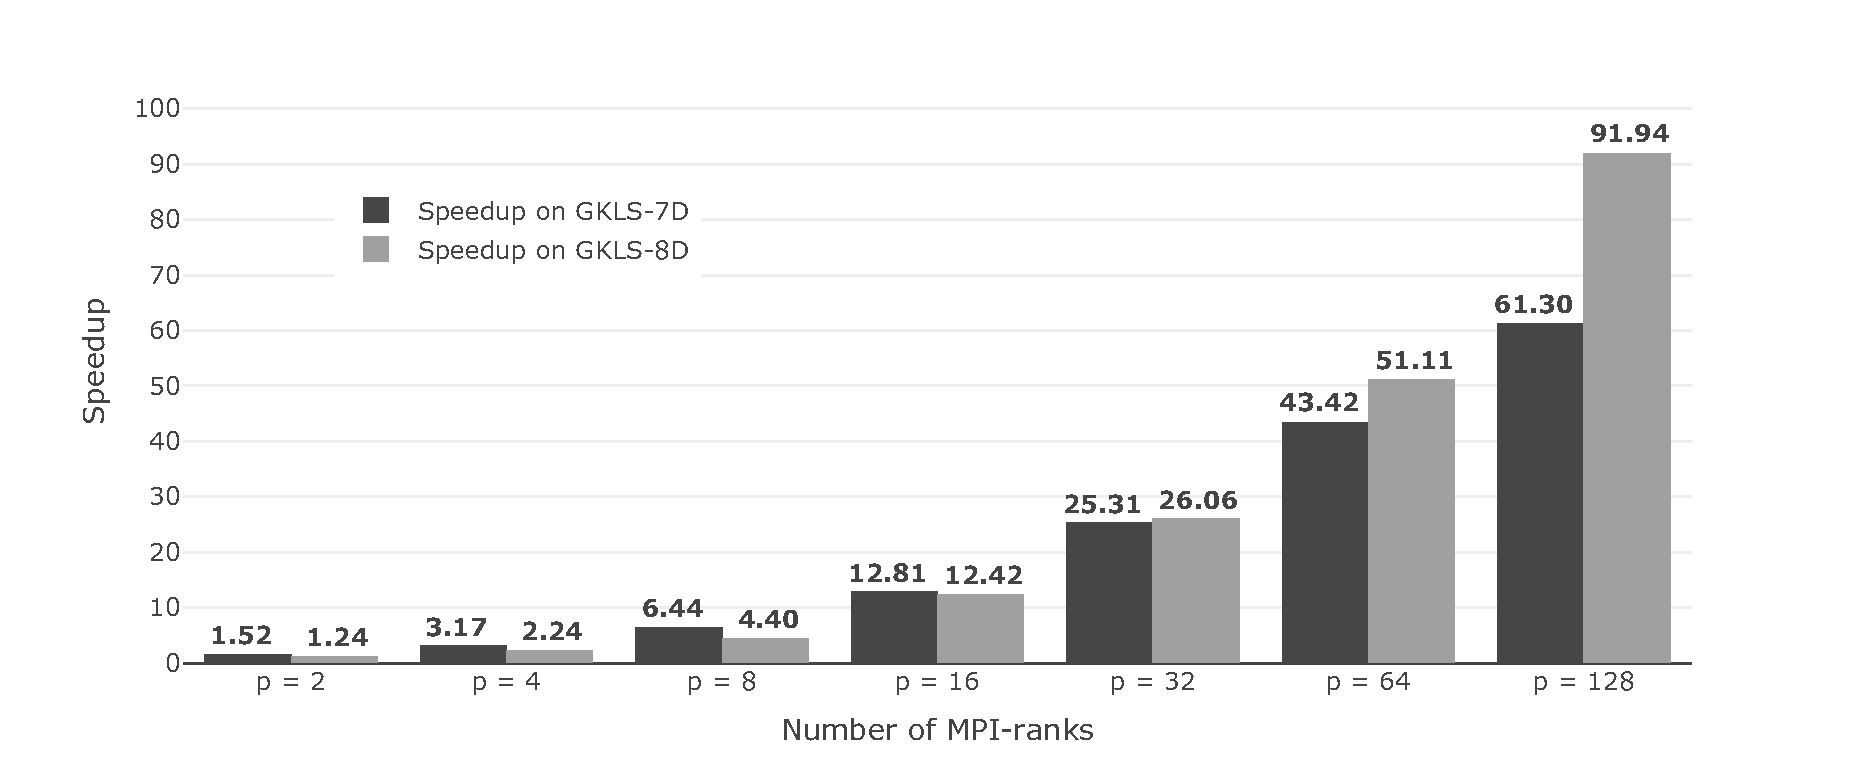
\includegraphics[width=1.05\linewidth]{figures/figure_5_12.pdf}
\caption{Speed-up of the asynchronous adaptive scheme.}
\label{fig:5_12}    
\end{figure}

Presented results demonstrate the substantial acceleration of the optimization process if to use the parallel adaptive scheme. It should be noted that if the parallelism is realized  with  few number of ranks then the efficiency of parallelizing is better for problems of the less dimension, however, the growth of number of MPI ranks leads to increasing the speed-up for  problems with more dimension (for 128 ranks speed-up in 8-dimensional problems is almost 1.5 times more than in 7-dimensional case).

\begin{thebibliography}{99.}
\bibitem{5_BarkGer2014} Barkalov, K.A., Gergel, V.P.: Multilevel scheme of dimensionality reduction for parallel global search algorithms.  OPT-i 2014 -- 1st International Conference on Engineering and Applied Sciences Optimization, Proceedings, 2111--2124 (2014)
\bibitem{5_BarkGerLeb} Barkalov, K., Gergel, V., Lebedev, I.: Solving global optimization problems on GPU cluster  AIP Conference Proceedings \textbf{1738}, 400006 (2016)
\bibitem{5_BarkLeb} Barkalov, K., Lebedev, I.: Local tuning in multilevel scheme of parallel global optimization.  AIP Conference Proceedings \textbf{1776}, 060006 (2016)
\bibitem{5_CarrHowe}	Carr, C.R., Howe, C.W.: Quantitative Decision Procedures in Management and Economic: Deterministic Theory and Applications. McGraw-Hill, New York (1964)
\bibitem{5_Evtushenko}	Evtushenko, Yu.G.: Numerical Optimization Techniques. Translation Series in Mathematics and Engineering. Optimization Software  Inc., Publication Division, New York (1985)
\bibitem{5_GavianoKvasovLeraSergeyev} Gaviano, M., Kvasov, D.E., Lera, D., Sergeyev, Y.D.: Algorithm 829: Software for generation of classes of test functions with known local and global minima for global optimization. ACM Trans. Math. Software \textbf{29}(4), 469–480 (2003)
\bibitem{5_GerGriIsr} Gergel, V.,  Grishagin, V., Israfilov, R.: Local tuning in nested scheme of global optimization, Procedia Computer Science \textbf{51}, 865--874 (2015) 
\bibitem{5_GerGriGer}	Gergel, V., Grishagin, V., Gergel, A.: Adaptive nested optimization scheme for multidimensional global search, J. Glob. Opt. \textbf{66}, 35–51 (2016).
\bibitem{5_GrishaginOperChar}  Grishagin,V.A.: Operation characteristics of some global search algorithms, Problems of Statistical Optimization \textbf{7},  198--206 (1978). In Russian
\bibitem{5_GriIsrAIP}	Grishagin, V.A., Israfilov, R.A.: Global search acceleration in the nested optimization scheme. AIP Conf. Proc. \textbf{1738}, 400010 (2016)
\bibitem{5_GriIsrSergAIP} Grishagin, V., Israfilov, R., Sergeyev, Y.: Comparative efficiency of dimensionality reduction schemes in global optimization. AIP Conf. Proc. \textbf{1776}, 060011 (2016)
\bibitem{5_GriIsrSergAMC}	Grishagin, V.,  Israfilov, R., Sergeyev, Y.: Convergence conditions and numerical comparison of global optimization methods based on dimensionality reduction schemes. Appl. Math.  Comput. \textbf{318}, 270--280 (2018)
\bibitem{5_GriIsrCEUR}Grishagin, V.A., Israfilov, R.A.: Multidimensional Constrained Global Optimization in Domains with Computable Boundaries. CEUR Workshop Proceedings \textbf{1513}, 75--84 (2015)
\bibitem{5_GriKvaMukhStr} Grishagin, V.A., Kvasov, D.E., Mukhametzhanov, M.S., Strongin, R.G.: Information and characteristical global search algorithms. This volume.
\bibitem{5_GrishaginSergeyevStrongin} Grishagin, V.A., Sergeyev, Y.D., Strongin, R.G.: Parallel characteristical algorithms for solving problems of global optimization. J. Global Optim. \textbf{10}(2), 185–206 (1997)
\bibitem{5_GrishaginStrongin_EnginCybernetics} Grishagin, V.A., Strongin, R.G.: Optimization of multiextremal functions subject to monotonically unimodal constraints. Engineering Cybernetics \textbf{22},  117--122 (1984)
\bibitem{5_Jones}Jones, D.R.: The DIRECT global optimization algorithm. In: C.A. Floudas, P.M. Pardalos
(eds.) Encyclopedia of Optimization, vol. 1, pp. 431–440. Kluwer Academic Publishers, Dordrecht (2001)
\bibitem{5_JonesPerttunenStuckman}Jones, D.R., Perttunen, C.D.,   Stuckman, B.E.: Lipschitzian optimization
without the Lipschitz constant, J. Optim. Theory Appl. 79,  157--181 (1993)
\bibitem{5_Kushner}	Kushner, H.J.: A new method of locating the maximum point of an arbitrary multipeak curve in the presence of noise. Transactions of ASME, Ser. D. Journal of Basic Engineering \textbf{86}, 97--106 (1964)
\bibitem{5_Locatelli} Locatelli, M.: Bayesian algorithms for one-dimensional global optimization. Journal of Global Optimization \textbf{1}, 57--76 (1997)
\bibitem{5_LucidiPiccioni} Lucidi, S., Piccioni, M.:  Random tunneling by means of acceptance-rejection sampling for global optimization. J. Optim. Theory Appl. \textbf{62}(2), 255--277 (1989)
\bibitem{5_Mockus1980} Mockus, J.: The simple Bayesian algorithm for the multidimensional global optimization. In: Archetti, F., and Cugiani, M. (Eds.) Numerical Techniques for Stochastic Systems. North-Holland, Amsterdam,
the Netherlands (1980)
\bibitem{5_Mockus1988}	Mockus, J.: Bayesian Approach to Global Optimization. Kluwer Academic Publishers, Dordrecht (1988)
\bibitem{5_MockusEddy_et_al} Mockus, J., Eddy, W., Mockus, A., Mockus, L., Reklaitis, G.: Bayesian Heuristic Approach
to Discrete and Global Optimization. Kluwer Academic Publishers, Dordrecht (1996)
\bibitem{5_Piyavskij}	Piyavskij, S.A.: An Algorithm for Finding the Absolute Extremum of a Function. USSR Comput. Math. Math. Phys. \textbf{12}(4), 57--67 (1972)
\bibitem{5_SergeyevLocTun} Sergeyev, Y.D.: An information global optimization algorithm with local tuning. SIAM J. Optim. \textbf{5}(4), 858–870 (1995)
\bibitem{5_Sergeyev1998} Sergeyev, Y.D.: Global one-dimensional optimization using smooth auxiliary functions. Math. Program. \textbf{81}(1), 127–146 (1998)
\bibitem{5_SergeyevGrishaginOMS} Sergeyev, Y.D., Grishagin, V.A.: Sequential and parallel algorithms for global optimization, Optim. Methods Softw. \textbf{3},  111--124 (1994)
\bibitem{5_SergGriJCAA}	Sergeyev, Y.D., Grishagin, V.A.: Parallel Asynchronous Global Search and the Nested Optimization Scheme. J. Comp. Analysis Appl. \textbf{3}, 123--145 (2001)
\bibitem{5_SergMukhKvasLera} Sergeyev, Y.D., Mukhametzhanov, M.S., Kvasov, D.E., Lera, D.: Derivative-free local tuning and local improvement techniques embedded in the univariate global optimization. J. Optim. Theory Appl. 171(1), 186--208 (2016)
\bibitem{5_ShiOlaf}   Shi, L., {\'O}lafsson, S.: Nested Partitions Method for Global Optimization. Operations Research \textbf{48}, 390--407 (2000)
\bibitem{5_Shubert} Shubert, B.O.: A sequential method seeking the global maximum of a function. SIAM J. Numer. Anal. \textbf{9}(3), 379–388 (1972)
\bibitem{5_StrMonRus}	Strongin, R.G.: Numerical Methods in Multiextremal Problems (Information-Statistical Algorithms). Nauka, Moscow (1978). In Russian
\bibitem{5_Str1973} Strongin, R.G.: On the convergence of an algorithm for finding a global extremum. Engineering Cybernetics 11, 549–555 (1973)
\bibitem{5_StrMarkin} Strongin, R.G., Markin, D.L.: Minimization of multiextremal functions with nonconvex constraints. Cybernetics 22, 486–493 (1986)
\bibitem{5_StrSergMon2000} Strongin, R.G., Sergeyev, Y.D.: Global Optimization with Non-Convex Constraints. Sequential and Parallel Algorithms. Kluwer Academic Publishers, Dordrecht (2000) 
\bibitem{5_SysoyevBarkGerLeb} Sysoyev, A., Barkalov, K., Gergel, V., Lebedev, I.: MPI implementation of dimension reduction multilevel scheme for parallel solving the global optimization problems  CEUR Workshop Proceedings \textbf{1482}, 61--68 (2015)
\bibitem{5_vanDam}	van Dam, E.R., Husslage, B., Hertog, D. One-dimensional Nested Maximin Designs. J. Glob. Opt. \textbf{46}, 287--306 (2010)
\bibitem{5_Zilinskas1975} $\check{Z}$ilinskas, A.: One-step Bayesian method for the search of the optimum of one-variable functions. Cybernetics 1, 139--144 (1975)
\bibitem{5_Zilinskas1981} $\check{Z}$ilinskas, A.: Two algorithms for one-dimensional multimodal minimization. Mat. Operationsforsch. Statist. \textbf{12}, Ser. Optimization, 53--63 (1981)
\bibitem{5_Zilinskas1985} $\check{Z}$ilinskas, A.: Axiomatic characterization of a global optimization algorithm and investigation of its search strategy. Operations Research Letters \textbf{4}, 35--39 (1985)
\end{thebibliography}

%\end{document}
%%%%%%%%%%%%%%%%%%%% author.tex %%%%%%%%%%%%%%%%%%%%%%%%%%%%%%%%%%%
%
% sample root file for your "contribution" to a contributed volume
%
% Use this file as a template for your own input.
%
%%%%%%%%%%%%%%%% Springer %%%%%%%%%%%%%%%%%%%%%%%%%%%%%%%%%%%%%%%%%


%% RECOMMENDED %%%%%%%%%%%%%%%%%%%%%%%%%%%%%%%%%%%%%%%%%%%%%%%%%%%
%\documentclass[graybox]{svmult}
%
%% choose options for [] as required from the list
%% in the Reference Guide
%
%\usepackage{mathptmx}       % selects Times Roman as basic font
%\usepackage{helvet}         % selects Helvetica as sans-serif font
%\usepackage{courier}        % selects Courier as typewriter font
%\usepackage{type1cm}        % activate if the above 3 fonts are
                             % not available on your system
%
%\usepackage{makeidx}         % allows index generation
%\usepackage{graphicx}        % standard LaTeX graphics tool
%                             % when including figure files
%\usepackage{multicol}        % used for the two-column index
%\usepackage[bottom]{footmisc}% places footnotes at page bottom
%\usepackage{amsmath}

%\usepackage[colorlinks=true]{hyperref}
%\hypersetup{urlcolor=blue, citecolor=red}


%% see the list of further useful packages
%% in the Reference Guide
%
%\makeindex             % used for the subject index
%                       % please use the style svind.ist with
%                       % your makeindex program
%
%%%%%%%%%%%%%%%%%%%%%%%%%%%%%%%%%%%%%%%%%%%%%%%%%%%%%%%%%%%%%%%%%%%%%%%%%%%%%%%%%%%%%%%%%%
%
%\begin{document}

\title{Parallel computations for the multidimensional multiextremal optimization problems with the dimensionality reduction using Peano curves }
\titlerunning{Parallel computations for the multidimensional optimization} 

\author{Konstantin Barkalov, Victor Gergel, Roman Strongin}
\authorrunning{K. Barkalov, V.Gergel, R. Strongin} 

\institute{Konstantin Barkalov,  Victor Gergel, Roman Strongin \at Lobachevsky State University of Nizhni Novgorod,  Nizhni Novgorod, Russia \email{konstantin.barkalov@itmm.unn.ru}}
%
% Use the package "url.sty" to avoid
% problems with special characters
% used in your e-mail or web address
%
\maketitle

\abstract*{The paper considers dimensionality reduction scheme based on Peano-type space-filling cures (evolvents). The initial multidimensional optimization problem is substituted by an equivalent one-dimensional one based on the application of the mapping of a multidimensional search domain onto a segment of the real axis. A general description of the approach and its substantiations are given. The development of the classical scheme based on the application of a set of mappings and the implementation of new types of evolvents is considered for the parallel algorithm.}

\abstract{The paper considers dimensionality reduction scheme based on Peano-type space-filling cures (evolvents). The initial multidimensional optimization problem is substituted by an equivalent one-dimensional one based on the application of the mapping of a multidimensional search domain onto a segment of the real axis. A general description of the approach and its substantiations are given. The development of the classical scheme based on the application of a set of mappings and the implementation of new types of evolvents is considered for the parallel algorithm.}

\section{General approach scheme}

Let us consider a multidimensional global optimization problem
\begin{equation}\label{6_problem} 
\varphi(y^\ast)=\min{\left\{\varphi(y):y\in D, \; g_j(y)\leq 0, \; 1 \leq j \leq m\right\}},
\end{equation} 
\begin{equation}\label{6_D}
D=\left\{y\in R^N: -2^{-1}\leq y_i \leq 2^{-1}, 1\leq i \leq N \right\}.
\end{equation}
This problem statement covers a large class of problems since any hyperinterval 
\[
S=\left\{y\in R^N: a_i\leq y_i \leq b_i, 1\leq i \leq N\right\}
\]
can be reduced to the  hypercube (\ref{6_D}) by linear transformation of coordinates.

There is a number of ways to adapt efficient one-dimensional algorithms for solving multidimensional problems; see, for example, the diagonal partitions method in \cite{6_Sergeyev2006,6_Sergeyev2015,6_Sergeyev2017} or the simplicial partitions method in \cite{6_Zilinskas2008,6_Zilinskas2014,6_Zilinskas2014_1}. 

The dimensionality reduction method described below uses a mapping of a multidimensional search domain onto a one-dimensional interval by means of so called \textit{Peano curves}. Peano, an Italian mathematician, has found that an single-valued continuous mapping $y(x)=(y_1(x),y_2(x))$ of the interval $[0,1]$ onto the square 
\[
\left\{y\in R^2: -2^{-1}\leq y_1,y_2 \leq 2^{-1} \right\} = \left\{ y(x): 0 \leq x \leq 1 \right\}
\]
can be constructed.
This result was generalized onto a multidimensional case, i.e., the existence of the curves $y(x)$ defined by continuous coordinate functions $y_i(x), \; x \in [0,1],\; 1 \leq i \leq N,$ and mapping uniquely the unit interval $[0,1]$ onto a $N$-dimensional hypercube 
\[
D=\left\{y\in R^N: -2^{-1}\leq y_i \leq 2^{-1}, 1\leq i \leq N \right\} = \left\{ y(x): 0 \leq x \leq 1 \right\}
\]
had been proven. These curves, called also \textit{Peano curves}, allow to reduce a multidimensional constrained optimization problem over the domain $D$ to a one-dimensional constrained minimization problem over the unit interval $[0,1]$
\begin{equation}\label{6_problem_1} 
\varphi(y(x^\ast))=\min{\left\{\varphi(y(x)):x\in [0,1], \; g_j(y(x))\leq 0, \; 1 \leq j \leq m\right\}}.
\end{equation} 

The considered dimensionality reduction scheme juxtaposes to a multidimensional problem with Lipschitz objective function and Lipschitz constraints a one-dimensional problem, where the corresponding functions satisfy uniform H\"{o}lder condition (see \cite{6_Strongin2000,6_Strongin2013}), i.e.,
\begin{equation}\label{6_Holder}
\left|g_j(y(x'))-g_j(y(x''))\right| \leq K_j \left|x'-x''\right|^{1/N}, \; x',x''\in [0,1], \; 1\leq j \leq m+1. 
\end{equation}
Here $N$ is the dimensionality of the initial multidimensional problem and the coefficients $K_j$ are related with Lipschitz constant $L_j$ of the initial problem as 
\[
K_j \leq 2L_j \sqrt{N+3},\; 1\leq j \leq m+1.
\]
Some issues of H\"older functions optimization are considered in \cite{6_Gourdin,6_Lera2002,6_Lera2010,6_Hime,6_Lera2015}.

We will consider initial problem (\ref{6_problem}) assuming that the problem functions $g_j(y),\; 1 \leq j \leq m+1,$ may be defined partially. This means that they are defined and computable only in the subranges $Q_j \in [0,1]$, 
\begin{equation}\label{6_Q}
Q_1=[0,1], \; Q_{j+1}=\left\{x \in Q_j : g_j(y(x)) \leq 0 \right\}, \; 1 \leq j \leq m.
\end{equation}
These conditions allows to introduce a classification of the points $x \in [0,1]$ according to the number $\nu = \nu(x)$ of the constraints computed at this point. The index $\nu(x)$ can also be defined by the conditions
\begin{equation}\label{6_nu}
g_j(y(x)) \leq 0, \; 1 \leq j < \nu, \; g_\nu(y(x))>0,
\end{equation}
where the last inequality is inessential if $\nu=m+1$.

Therefore, the execution of an iteration at the point $x \in [0,1]$ is reduced to the successive computation of the values $g_j(y(x)),\; 1 \leq j \leq \nu(x),$ i.e., the next value $g_{j+1}(y(x))$ is computed if and only if $g_j(y(x)) \leq 0$. The process of computations is terminated either as a result of occurrence of the inequality $g_j(y(x))>0$ or by satisfying the equality $\nu(x)=m+1$. Moreover, the described procedure called the trial at the point $x \in [0,1]$ leads automatically to determining the index $\nu$ of this point. %since conditions (\ref{6_nu}) are equivalent to the inequalities 
The pair of values 
\[
\nu=\nu(x), \; z=g_\nu(y(x)),
\]
generated by the trial at the point $x \in [0,1]$, is called \textit{the trial result}.

Besides the exact solution $y^\ast$ from (\ref{6_problem}) let us consider also the \textit{$\epsilon$-reserved solution} of the problem (\ref{6_problem}) defined by the conditions 
\begin{equation}\label{6_eps_r}
\varphi(y_\epsilon) = \min \left\{ \varphi(y): \; y \in D, \; g_j(y) \leq -\epsilon_j, \; 1 \leq j \leq m \right\},
\end{equation}
where $\epsilon_1,...,\epsilon_m$ are the positive values (the ``reserves'' with respect to each constraint). Let us introduce into the consideration also the set
\begin{equation}\label{6_eps_solution}
Y_\epsilon =  \left\{ y \in D: \; g_j(y) \leq 0, \; 1 \leq j \leq m, \; \varphi(y) \leq \varphi(y_\epsilon) \right\}
\end{equation}
of all feasible points of problem (\ref{6_problem}), which are not worse (with respect to the objective function value) than the $\epsilon$-reserved solution. Fig.~\ref{6_fig_1} illustrates the definition introduced.

\begin{figure}[t]
%\sidecaption[t]
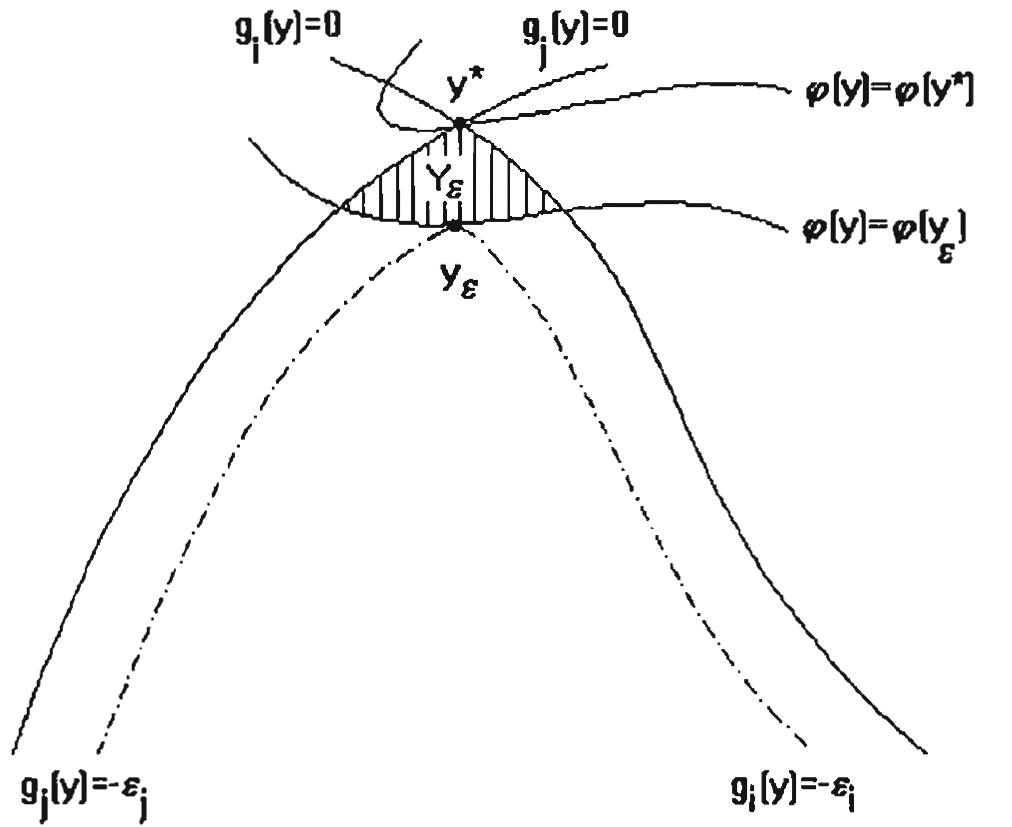
\includegraphics[width=0.7\linewidth]{figures/6_1.png}
\caption{$\epsilon$-reserved solution}
\label{6_fig_1}     
\end{figure}

The existence of the $\epsilon$-reserved solution of problem (\ref{6_problem}) can be interpreted as an analog of the regularity conditions in the classical problems of nonlinear programming. It should be noted also the applied importance of this condition. Even if the exact solution $y^\ast$ is known, its practical realization is possible as some approximation of $y^\ast$ only. Therefore, it is important that there exist the points from the feasible domain $Q$ close to $y^\ast$ (with respect to the coordinates and values). The existence of the $\epsilon$-reserved solution guarantees the existence of such points. In this case, the domain $Y_\epsilon$ can play a role of the set of suitable approximations.

Prior to going to the detailed description of the Peano curves and of the algorithm, let us consider some properties of reduced problem (\ref{6_problem_1}), which are absent in the pure one-dimensional case. First, as it has been already mentioned above, the functions $g_j(y(x)), \; 1 \leq j \leq m+1,$ are not Lipschitzian. They satisfy H\"older condition. Consequently, all the interval lengths in the search algorithm rules have to be replaced by the lengths in the metric
\[
\rho (x',x'') = \left(\left|x'-x''\right|\right)^{1/N}, \; x',x'' \in [0,1].
\]
Second, in general, sets (\ref{6_Q}) being the inverse images of the essentially non-cubic $N$-dimensional subsets with the nonlinear boundaries $g_j(y)=0, \; y \in D, \; 1\leq j \leq m,$ are not the finite unions of $x$-intercepts. Consequently, taking into account the $\epsilon$-reserved solutions plays a significantly more important role for the convergence in the reduced univariate problem (\ref{6_problem_1}) than in the pure one-dimensional case.

The issues of the numerical construction of the Peano-type space filling curves and the corresponding theory are considered in details in \cite{6_Butz,6_Sagan,6_Strongin2000,6_Strongin2013}. Here we will describe the basic steps of constructing a curve mapping a unit interval of the real axis $[0,1]$ onto a hypercube  
\[
D=\left\{y\in R^N: -2^{-1}\leq y_i \leq 2^{-1}, 1\leq i \leq N \right\}.
\]

\begin{enumerate}
	\item 
A hypercube $D$ with the unit edge length is divided by the coordinate hyperplanes into $2^N$ hypercubes of the first partition (with the edge length equal to $1/2$), which are indexed by the numbers $z_1$ ranging from $0$ to $2^N-1$. Let us agree to designate the hypercube of the first partition with the index $z_1$ as $D(z_1)$.

Next, each hypercube of the first partition is also divided into $2^N$ hypercubes of the second partition (with the edge length equal to $1/4$) by the hyperplanes parallel to the coordinate axes and crossing the middles of the hypercube edges orthogonal to these hyperplanes. The hypercubes of the second partition  included in the hypercube $D(z_1)$ are indexed by the numbers $z_2$ ranging from $0$ to $2^N-1$. The hypercube of the second partition  with the index $z_2$ from  $D(z_1)$ is denoted as $D(z_1, z_2)$. The case of $N=2$ is presented in Fig.~\ref{6_fig_2} for $m=1$, $m=2$.

\begin{figure}
\begin{minipage}{0.5\linewidth}
\center{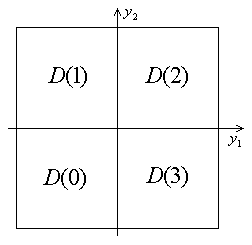
\includegraphics[width=0.9\linewidth]{figures/6_2a.png} \\ $m=1$}
\end{minipage}
\hfill
\begin{minipage}{0.5\linewidth}
\center{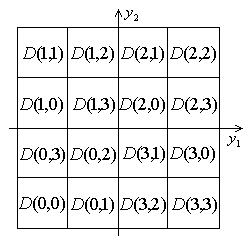
\includegraphics[width=0.9\linewidth]{figures/6_2b.png} \\ $m=2$}
\end{minipage}
\caption{The partition of an $N$-dimensional hypercube}
\label{6_fig_2}
\end{figure}

Continuing this process, one can construct the hypercubes of any $m$-th partition with the edge length equal to $(1/2)^m$, which are denoted as $D(z_1,...,z_m)$. It is obvious, that $D(z_1) \supset D(z_1,z_2) \supset ... \supset D(z_1,...,z_m)$ and $0 \leq z_j \leq 2^N-1$, \mbox{$1 \leq j \leq m$}.

\item
Now let us perform the division of the interval $[0,1]$ into $2^N$ equal parts, each of them also is divided into $2^N$ equal parts, etc. The elements of each partition are indexed from the left to the right by the numbers $z_j$ ranging from $0$ to \mbox{$2^N-1$} where $j$ is the index of subdivision. Let us denote the intervals of the $m$-th partition as $d(z_1,...,z_m)$ where, for example, $d(z_1,z_2)$ means the interval of the second partition with the index $z_2$ being a part of the interval $d(z_1)$ of the first partition with the index $z_1$.

One can note that  $d(z_1) \supset d(z_1,z_2) \supset ... \supset d(z_1,...,z_m)$ and the length of the interval $d(z_1,...,z_m)$ is equal to  $(1/2)^{mN}$. An interval $d(z_1,...,z_m)$ is supposed to include its left hand end. It contains its right hand boundary if and only if when $z_1=z_2=...=z_m=2^N-1$. The case of $N=2$ is presented in Fig.~\ref{6_fig_3} for $m=1$ and $m=2$.

\begin{figure}[t]
%\sidecaption[t]
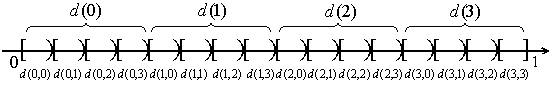
\includegraphics[width=0.9\linewidth]{figures/6_3.png}
\caption{Partition of a one-dimensional interval}
\label{6_fig_3}     
\end{figure}

\item
Assume that the point $y(x) \in D$ corresponding to the point $x \in [0,1]$ for any $m \geq $ belongs to the hypercube $D(z_1,...,z_m)$ if $x$ falls into the interval $d(z_1,...,z_m)$, i.e.,
\[
x \in d(z_1,...,z_m) \rightarrow y(x) \in D(z_1,...,z_m).
\]
The constructed correspondence  $y(x)$ is single-valued.
\item
In order to provide the continuity of the constructed correspondence, let us impose the following requirements on the indexing order of the hypercubes of each partition. Since $2^{mN}$ centers $y(z_1,...,z_m)$ of the hypercubes of the $m$-th partition $D(z_1,...,z_m)$ form a uniform orthogonal grid in the domain $D$ (the step of this grid with respect to any coordinate is equal to $2^{-m}$), one can introduce the following numeration of the grid nodes. Let us enumerate from the left to the right by index $i$ all subintervals of the $m$- 	th partition in the interval $[0,1]$, i.e.,
\[
d(z_1,...,z_m)=[x_i, x_{i+1}), \; 0 \leq i < 2^{mN}-1,
\]
were the left end of the $i$-th interval is denoted as $x_i$.

Assume the center of the hypercube $D(z_1,...,z_m)$ to have the same index $i$ as the interval $d(z_1,...,z_m)$ corresponding to this hypercube, i.e.,
\[
y_i = y(z_1,...,z_m), \; 0 \leq i < 2^{mN}-1.
\]
The centers $y_i$ and $y_{i+1}$ correspond to the adjacent hypercubes having a common facet. More details on the indexing of the hypercubes can be found in \cite{6_Strongin2013}.
\end{enumerate}

Let us consider the mapping  $l(x)$ of the interval $[0,1]$ into a hypercube $D$ defined by the expression 
\[
l(x)=y_i+(y_{i+1}-y_i)\frac{w(x)-x_i}{x_{i+1}-x_i}, \; x_i \leq w(x) \leq x_{i+1},
\]
\[
w(x)=x(1-2^{-mN}), \; 0 \leq x \leq 1.
\]
The image of any subinterval
\[
\left[x_i(1-2^{-mN})^{-1}, x_{i+1}(1-2^{-mN})^{-1}\right], \; 0 \leq i < 2^{mN}-1
\]
of the interval $[0,1]$ for the correspondence $l(x)$ is a linear segment connecting the nodes $y_i$ and $y_{i+1}$.

Thus, we have built a piecewise linear curve $l_m(x), 0 \leq x \leq 1,$ connecting the nodes $y_i, 0 \leq i< 2^{mN}-1,$ in the order of their indexing. This curve obtained numerically (\textit{the evolvent})  is an approximation of the theoretical Peano curve with the precision not worse than $2^{-m}$ with the respect to each coordinate (the parameter m is called\textit{ the density of the evolvent}). As an illustration, an image of the interval $[0,1]$ for the mapping $l_m(x)$ in the case $N=2, m=3$ is presented in Fig.~\ref{6_fig_4}. The grid nodes are marked with the dark circles. 

\begin{figure}[t]
%\sidecaption[t]
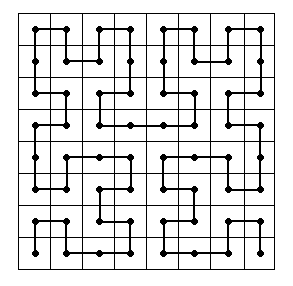
\includegraphics[width=0.5\linewidth]{figures/6_4.png}
\caption{A piecewise linear curve}
\label{6_fig_4}     
\end{figure}

\section{Multidimensional generalized global search algorithm}
The considered dimensionality reduction scheme associates a multidimensional problem with Lipschitz objective function and Lipschitz constraints with a one-dimensional problem, where the corresponding functions satisfy uniform H\"older condition (\ref{6_Holder}). As result, all lengths of the intervals appearing in the rules of the search algorithm should be replaced by the lengths in a new metrics, where the distance is defined by the expression
\[
\Delta_i = \left|x_i-x_{i-1}\right|^{1/N}.
\]
Also, in the reduction of the problem dimensionality by Peano curve  $y(x), 0 \leq x \leq 1,$ a trial at a point $x^k \in [0,1]$ executed at the $k$-th iteration of the algorithm will consist in the following sequence of operations.
\begin{itemize}
	\item Determine the image  $y^k=y(x^k)$ in accordance with the mapping  $y(x)$.
	\item Compute the values  $g_1(y^k),...,g_\nu(y^k)$, where the index $\nu \leq m$ are determined by the conditions
	\[
	g_j(y^k)\leq 0, \; 1 \leq j<\nu, \; g_\nu(y^k)>0, \; \nu \leq m.
	\]
	The occurrence of the first violation of the constraint terminates the trial at the point $y^k$. In the case, when the point $y^k$ is a feasible one, i.e., when $y(x^k) \in Q_{m+1}$, the trial includes the computation of the values of all functions of the problems and the index is accepted to be $\nu = m+1$. The pair of values
	\begin{equation}\label{6_trial_res}
	\nu = \nu(x^k), \; z^k = g_\nu(y(x^k))
	\end{equation}
	is a \textit{result of the trial} at the point $x^k$.
\end{itemize}

Thus, one can easily modify the initial one-dimensional algorithm and obtain on this base a multidimensional \textit{generalized index global search algorithm}, described below.

The first trial is executed at an arbitrary internal point $x^1 \in (0,1)$. The selection of the point $x^{k+1}, k \geq 1,$ of any next trial is determined by the following rules.

Rule 1. Renumber the points $x^1,...,x^k$ of the preceding trials by the
lower indices in ascending order of coordinate values, i.e.
\begin{equation}\label{6_trial_points}
0=x_0<x_1<\dots <x_k<x_{k+1}=1,
\end{equation}
and juxtapose to them the values $z_i=g_\nu(y(x_i)), \; \nu=\nu(x_i), \; 1 \leq i \leq k$, from (\ref{6_trial_res}) computed at these points. The points $x_0=0$ and
$x_{k+1}=1$ are introduced additionally for the convenience of further notations, while the values $z_0$ and
$z_{k+1}$ are not defined.

Rule 2. Classify the indices $i, \; 1 \leq i \leq k$, of the trial points (\ref{6_trial_points})
according to the number of the problem constraints fulfilled at these points by constructing the sets
\[
I_\nu =\left\{i:1 \leq i \leq k, \; \nu=\nu(x_i) \right\}, \; 1 \leq \nu \leq m+1,
\]
containing the numbers of all the points $x_i, \; 1 \leq i \leq k$, with
the same values of $\nu$. The end points $x_0=0$ and $x_{k+1}=1$ are
interpreted as the ones having indices equal to zero. An additional set $I_0=\left\{0,k+1\right\}$ corresponds to them.

Determine the maximum value of the index
\[
M=\max\left\{\nu(x_i), \; 1 \leq i \leq k \right \}.
\]

Rule 3. Compute the current lower estimates
\begin{equation}\label{6_mu}
\mu = \max\left\{ \frac{\left|z_i-z_j\right|}{ (x_i - x_j)^{1/N} }, \; i,j \in I_\nu, \; i>j \right\}
\end{equation}
for the unknown H{\"o}lder constants $K_\nu$ of the functions $g_\nu(y),1
\leq \nu \leq m+1$. If a set $I_\nu$ contains less than two elements, or
if $\mu_\nu$ from (\ref{6_mu}) is equal to zero, then assume $\mu_\nu=1$.

Rule 4. For all nonempty sets $I_\nu, \; 1 \leq \nu \leq m+1$, compute the
estimates
\[
z_\nu^\ast = \left\{
   \begin{array}{lr}
     -\epsilon_\nu, & \nu < M,\\
     \min\{ g_\nu(y(x_i)): i\in I_\nu \}, & \nu = M,
   \end{array}
\right.
 \]
where the vector $\epsilon_R = (\epsilon_1,...,\epsilon_m)$ is a predefined vector with the nonnegative components (\textit{the reserve vector}).

Rule 5. For each interval ($x_{i-1},x_i), \; 1 \leq i \leq k+1,$ compute
the \textit{characteristics} $R(i)$ :
\[
R(i)=2\Delta_i-4\frac{z_i-z_\nu^\ast}{r_\nu \mu_\nu}, \; \nu=\nu(x_i)>\nu(x_{i-1}),
\]
\begin{equation}%\label{eq:14}
R(i)=\Delta_i+\frac{(z_i-z_{i-1})^2}{r_\nu^2 \mu_\nu^2\Delta_i}-2\frac{z_i+z_{i-1}-2z_\nu^\ast}{r_\nu \mu_\nu}, \;  \nu=\nu(x_i)=\nu(x_{i-1}),
\end{equation}
\[
R(i)=2\Delta_i-4\frac{z_{i-1}-z_\nu^\ast}{r_\nu \mu_\nu}, \; \nu=\nu(x_{i-1})>\nu(x_i),
\]
where $\Delta_i=(x_i - x_{i-1})^{1/N}$. The values $r_\nu > 1, \; 1 \leq
\nu \leq m+1,$ are parameters of the algorithm. An appropriate selection
of $r_\nu$ allows to consider the product $r_\nu \mu_\nu$ as an estimate
of the H{\"o}lder constants $K_\nu, \; 1 \leq \nu \leq m+1$.

Rule 6. Find the interval $(x_{t-1},x_t)$ with the maximum characteristic
\begin{equation}\label{6_MaxR}
R(t)=\max{\left\{R(i): 1 \leq i \leq k+1\right\}}.
\end{equation}

Rule 7. Make the next trial at the midpoint of the interval
$(x_{t-1},x_t)$ if the indices of the points $x_{t-1}$ and $x_t$  are not
the same, i.e.,
\[
x^{k+1} = \frac{x_t + x_{t-1}}{2}, \; \nu(x_{t-1}) \neq \nu(x_t).
\]
Otherwise, make the trial at the point
\begin{equation}%\label{eq:142}
x^{k+1} = \frac{x_t+x_{t-1}}{2} - \frac{\mathrm{sign}(z_t-z_{t-1})}{2r_\nu}\left[\frac{\left|z_t-z_{t-1}\right|}{\mu_\nu}\right]^N, \; \nu=\nu(x_{t-1})=\nu(x_t).
\end{equation}

We may take as termination condition the inequality $\Delta_t \leq
\epsilon$, where $t$ is from (\ref{6_MaxR}) and $\epsilon>0$ is the
predefined accuracy.

\textbf{The algorithm convergence conditions.} These conditions are a special case of the convergence theorem which will be proved in Subsection 6.3 for the parallel algorithm with a single curve on a single processor.

\begin{example} \label{6_example1}
As an illustration, let us consider the problem of minimization of the function
\begin{align*}
 \varphi(y_1,y_2) = &-1.5y_1^2\exp(1-y_1^2-20.25(y_1-y_2)^2)- \\
				            &-(0.5(y_1-1)(y_2-1))^4\exp(2-(0.5(y_1-1))^4-(y_2-1)^4)
\end{align*}
within the domain $0 \leq y_1\leq 4,\ -1\leq y_2\leq 3$, with the constraints 
\begin{align*}
g_1(y_1,y_2)&=0.01((y_1-2.2)^2+(y_2-1.2)^2-2.25)\leq 0,\\
g_2(y_1,y_2)&=100(1-(y_1-2)^2/1.44-(0.5y_2)^2)\leq 0,\\
g_3(y_1,y_2)&=10(y_2-1.5-1.5\sin(6.283(y_1-1.75)))\leq 0.
\end{align*}

Fig.~\ref{6_fig_5} shows the square search domain and the points of $1098$ trials obtained by the index method with the following parameters: the reliability parameters $r_1=...=r_4=2$, the accuracy $\epsilon = 10^{-3}$, the evolvent density $m=12$.
\begin{figure}[t]
%\sidecaption[t]
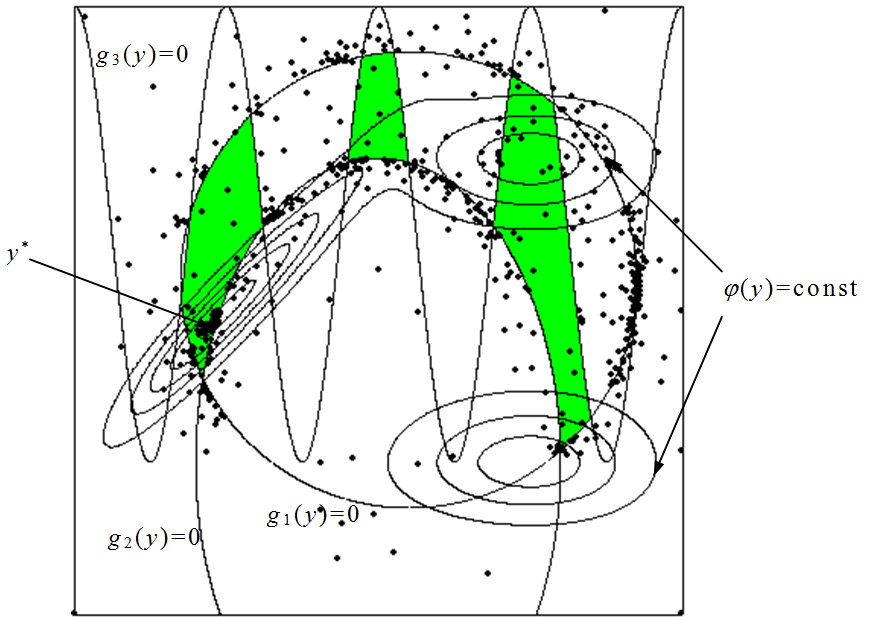
\includegraphics[width=0.8\linewidth]{figures/6_5.png}
\caption{The results of solving the test problem}
\label{6_fig_5}     
\end{figure}

\end{example}

Note that in applied problems, estimating the values of the constraints and of the objective functions very often requires considerable computation resources. The results of the experiments confirm the efficiency of the index scheme of the accounting for the constraints since the values of the functions $g_1,\ g_2,\ g_3,\ \varphi = g_4$ were computed $k_1=1098,\ k_2=623,\ k_3=392,$ and $k_4=152$ times, respectively. If the search of the solution were conducted on a uniform grid, in order to achieve the same accuracy $\epsilon=10^{-3}$ $k_1=1.6\cdot 10^7,\ k_2=7 \cdot 10^6,\ k_3=3\cdot 10^6,$ and $k_4=1.4 \cdot 10^6$ computations of the values of the functions $g_1,\ g_2,\ g_3,\ \varphi = g_4$, respectively, would be necessary.

\section{Parallel multidimensional multiextremal methods based on multiple Peano curves}

\subsection{Application of multiple mappings}\label{6_section_shift}

The reduction of the multidimensional problems to the one-dimensional ones using the Peano curves has such important properties as the continuity and the uniform boundedness of the function differences for limited variation of argument. However, a partial loss of information on the nearness of the points in the multidimensional space takes place since a point $x \in [0,1]$ has the left and the right neighbors only while the corresponding point $y(x) \in D \subset R^N$ has the neighbors in $2N$ directions. As a result, when using the mappings like Peano curve the images $y',\ y'',$ which are close to each other in the $N$-dimensional space can correspond to the preimages $x',\ x'',$ which can be far away from each other in the interval $[0,1]$. This property results in the excess computations since several limit points $x',\ x''$ of the trial sequence generated by the index method in the interval $[0,1]$ can correspond to a single limit point $y$ in the $N$-dimensional space.

One of the possible ways to overcome this disadvantage consists in using the multiple mappings
\begin{equation}%\label{eq:142}
Y_L(x)=\left\{y^0(x),\ y^1(x),...,\ y^L(x)\right\}
\end{equation}
instead of single Peano curve $y(x)$ (see \cite{6_Strongin1991,6_Strongin1992,6_Strongin2000}).

Let us consider a family of the hypercubes 
\begin{equation}\label{6_hypercubes}
D_l= \left\{y \in R^N: -2^{-1} \leq y_i+2^{-l} \leq 3 \cdot 2^{-1},\ 1\leq i\leq N\right\},\ 0 \leq l \leq L,
\end{equation}
where the hypercube $D_{l+1}$ is obtained by the translation of the hypercube $D_l$ along the main diagonal with displacement equal to $2^{-l}$ in each coordinate. In Fig.~\ref{6_fig_6} the hypercubes $D_0,...,D_3$ for the case $N=2,\ L=3$ are presented.

\begin{figure}[t]
%\sidecaption[t]
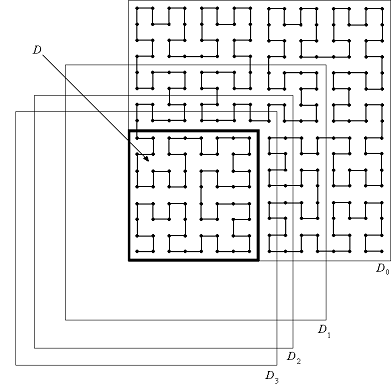
\includegraphics[width=0.7\linewidth]{figures/6_6.png}
\caption{Multiple mappings}
\label{6_fig_6}     
\end{figure}

Let us assume that the evolvent $y^0(x)$  maps the interval $[0,1]$ onto the hypercube $D_0$ from (\ref{6_hypercubes}), i.e.,
\[
D_0 = \left\{y^0(x) : x \in [0,1]\right\}.
\]
Then, the evolvents $y^l(x)=\left\{y_1^l(x),...,y_N^l(x)\right\}$, the coordinates of which are defined by the conditions 
\[
y_i^l(x)=y_i^{l-1}(x)+2^{-l},\ 1\leq i\leq N, \ 1\leq l\leq L,
\]
map the interval $[0,1]$ onto the corresponding hypercubes $D_l,\ 1\leq l \leq L$. In Fig.~\ref{6_fig_6} the image of the interval $[0,1]$ obtained by the curve $y^0(x),\ x\in [0,1],$ is shown as the broken line. Since the hypercube $D$ from (\ref{6_D}) is included in the common part of the family of hypercubes (\ref{6_hypercubes}) (the boundaries of hypercube $D$ are highlighted in Fig.~\ref{6_fig_6}), having introduced an additional constraint function
\begin{equation}\label{6_g0}
g_0(y)=\max\left\{\left|y_i\right| - 2^{-1}:\ 1\leq i\leq N\right\},
\end{equation}
one can present the initial hypercube $D$ in the form
\[
D=\left\{y^l(x):\; x\in [0,1],\ g_0(y^l(x))\leq 0 \right\},\ 0\leq l \leq L,
\]
i.e., $g_0(y) \leq 0$ if $y\in D$ and $g_0(y)>0$ otherwise. Consequently, any point $y \in D$ has its own preimage $x^l \in [0,1]$ for each mapping $y^l(x),\ 0\leq l\leq L$.

Thus, each evolvent $y^l(x),\ 0\leq l \leq L,$ generates its own problem of the type (\ref{6_problem_1}) featured by its own extended (in comparison with $D$) search domain $D_l$ and the additional constraint with the left hand part from (\ref{6_g0})
\begin{equation}\label{6_problem_l} 
\min{\left\{\varphi(y^l(x)):x\in [0,1], \; g_j(y^l(x))\leq 0, \; 0 \leq j \leq m\right\}}, \ 0 \leq l \leq L.
\end{equation} 

The problems (\ref{6_problem_l}) correspond to the domains $Q_0^l=[0,1]$ and $Q_{j+1}^l, 0 \leq j \leq m,$ defined by the expression 
\[
Q_{j+1}^l = \left\{x \in Q_j^l:g_j(y^l(x))\leq 0\right\},\ 0\leq j\leq m,
\]
for the corresponding evolvents $y^l(x)$. The application of a multiple mapping defines the following relation for the nearness in the multidimensional search domain and in the one-dimensional one.

\begin{theorem}
Let a point $y^\ast$ from the domain $D$ be contained in the line segment with the end-points $y',y'' \in D$ meeting the requirements 
\[
\left|y'_j - y''_j\right|\leq 2^{-p},\ y'_i=y''_i=y^\ast_i, \ 1\leq i \leq N,\ i \neq j,
\]
where $p$ is an integer  and $1\leq p \leq L$, i.e., the line segment is collinear with the $j$-th axis in $R^N$. Then, there exist at least one mapping $y^l(x),\ 0\leq l\leq L$, and the preimages $x^\ast,\; x',\; x''\in [0,1]$ such that
\[
y^\ast = y^l(x^\ast),\ y'=y^l(x'),\ y'' = y^l(x'')
\]
and
\[
\max \left\{ \left|x'-x^\ast\right|,\; \left|x''-x^\ast\right|,\; \left|x'-x''\right|\right\} \leq 2^{-pN}.
\]
\end{theorem}
\begin{proof}
Proof of this theorem is given in \cite{6_Strongin2000}.
\qed
\end{proof}

The conditions of the theorem single out a specific vicinity of the point $y^\ast$. This vicinity includes only the points, which can be obtained by the shift of $y^\ast$ parallel to one of the coordinate axes with a displacement not more than $2^{-p}$. By changing  $j,\ 1\leq j\leq N,$ in the theorem conditions it is possible to obtain the neighbours in any $N$ coordinate directions. According to the statement, the closeness of the points in the $N$-dimensional space in a particular direction will be reflected by the closeness of their preimages in one of the univariate problems. The information on the closeness of the points results, first, in more precise estimate of Lipschitz constants and, second, in the increase of the characteristics of the intervals, the images of the end points of which are close to each other in the $N$-dimensional space.

\subsection{Organization of the parallel computations}

Using the multiple mappings allows solving initial problem (\ref{6_problem}) by parallel solving $L+1$ problems of the type (\ref{6_problem_l}) on a set of intervals $[0,1]$ by the index method. Each univariate problem is solved on a separate processor. The results of trial at the point $x^k$ obtained on a particular processor for the problem being solved by this processor are interpreted as the results of the trials in the rest problems (in the corresponding points $x^{k0},\ x^{k1},...,x^{kL}$). In this approach, a trial at the point $x^k \in [0,1]$ executed in the framework of the $s$-th problem, consists in the following sequence of operations.
\begin{enumerate}
	\item Determine the image $y^k=y^s(x^k)$ at the mapping  $y^s(x)$.
	\item Compute the value $g_0(y^k)$. If $g_0(y^k) \leq 0$, i.e., if $y^k \in D$, then inform the rest processors on the start of the trial execution at the point $y^k$ (\textit{the blocking} of the point $y^k$).
	\item Compute the values $g_1(y^k),...,g_\nu(y^k),$ where the index $\nu \leq m$ are determined by the conditions
	\[
	g_j(y^k)\leq 0,\ 1\leq j< \nu,\ g_\nu(y^k) > 0,\ \nu \leq m.
	\]
	The occurrence of the first violation of any constraint terminates the trial at the point $y^k$. In the case when $y^k$ is a feasible one, i.e., when $y^s(x^k) \in Q_{m+1}$, the trial includes the computation of all functions of the problem. In this situation the index is set to $\nu = m+1$. The triplet
	\begin{equation}\label{6_triplet} 
	y^s(x^k),\ \nu = \nu(x^k),\ z^k=g_\nu(y^s(x^k))
	\end{equation}
	is  \textit{the trial result} at the point $x^k$.
	\item If $\nu (x^k)>0$, i.e., if $y^k \in D$, then determine the preimages $x^{kl} \in [0,1],\; 0\leq l \leq L,$ of the point $y^k$ and interpret the trial executed at the point $y^k \in D$ as the execution of the trials in the $L+1$ points 
	\[
	x^{k0},\ x^{k1},...,\ x^{kL}
	\]
	with the same result 
	\[
	\nu(x^{k0})=\nu(x^{k1})=...=\nu(x^{kL})=\nu(x^k),	
	\]
	\[
	g_\nu(y^0(x^{k0}))=g_\nu(y^1(x^{k1}))=...=g_\nu(y^L(x^{kL}))=z^k	
	\]
	and inform the rest processors on the results of the trial at the point $y^k$.	
	In the case if $\nu (x^k)=0$, i.e., if $y^k \notin D$, the trial result is related only to the $s$-th problem.	
\end{enumerate}

Each processor has its own copy of the software realizing the computations of the problem functions and the decision rule of the algorithm. For the organization of the interactions among the processors, $L+1$ queues are created on each processor, where the processors store the information on the iterations executed in the form of the triples (\ref{6_triplet}). Moreover, the index of the blocked point is assumed to be equal to $–1$; the function value at this point is undefined. The links among the processors by means of the queues $Q_{ls}$, where $l,\; 0\leq l \leq L,$ is the number of the transmitting processor and $s,\; 0 \leq s \leq L,$ is the index of the receiving processor, are illustrated in Fig.~\ref{6_fig_7}.

\begin{figure}[t]
%\sidecaption[t]
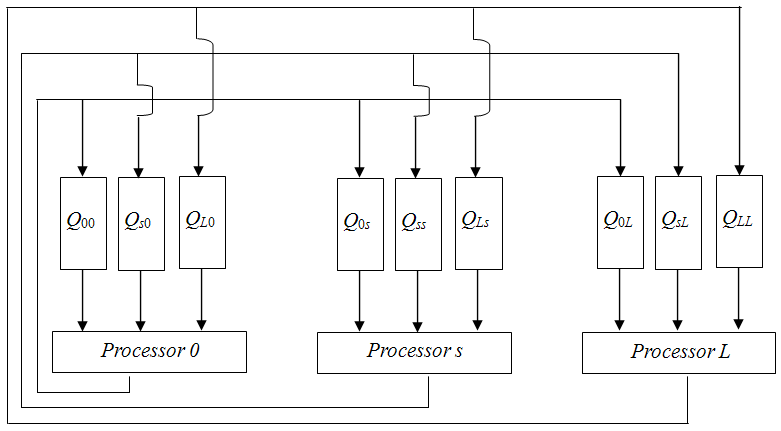
\includegraphics[width=0.8\linewidth]{figures/6_7.png}
\caption{The links among the processors }
\label{6_fig_7}     
\end{figure}

The proposed scheme does not include any managing processor that increases the reliability of the computations executed. The decision rules for the proposed parallel algorithm, in general, are the same as the rules of the sequential algorithm (except the method of the trial execution). However, in the purposes of deeper understanding of the subject, the scheme is presented here in full.

The algorithm for the selection of the iteration points is the same for all processors. The starting iteration is executed at a predefined point $x^1 \in (0,1)$ (the starting points for all processors are different). The selection of any next iteration point $x^{q+1}$, $q \geq 1$, is determined by the following rules.

Rule 1. Extract from all queues associated with $l$-th processor the results stored for this processor including the set of the iteration points $Y_q=\left\{y^{qi}:1 \leq i \leq s_q\right\}$,  the indices and the function values from (\ref{6_triplet}) computed at these points; determine the set $X_q={x^qi:1\leq i \leq s_q}$ of preimages of the points from the set $Y_q$ for the evolvent $y^l(x)$.

Rule 2. Renumber the points of the set of iterations
\[
\{x_1\} \cup X_1 \cup ... \cup X_q
\]
by the subscripts in increasing order of the coordinate
\begin{equation}\label{6_points_x} 
	0=x_0<x_1< \dots <x_k<x_{k+1}=1,
\end{equation}
where $k=1+s_1+\dots+s_q$, and juxtapose to them the values $z_i=g_\nu(x_i)$, $\nu = \nu(x_i)$, $1 \leq i \leq k$, computed at these points. The index of the blocked point $x_i$ (i.e., of the point, where other trial has been already started by other processor) is set to $–1$, i.e., $\nu(x_i)=-1$ and the value $z_i$ is undefined. The points $x_0,\ x_{k+1}$ are introduced additionally for the convenience of further presentation, the indices of these points are set to $-2$, i.e., $\nu(x_0)=\nu(x_{k+1})=-2$ and the values $z_0,\ z_{k+1}$ are undefined.

Rule 3. Perform the classification of the subscripts $i,\ 1 \leq i \leq k,$ of the points from (\ref{6_points_x}) in accordance with  the number of problem constraints fulfilled in these points by constructing the sets
\[
I_{-2} = \{0, k+1\},
\]
\[
I_{-1} = \{i: 1 \leq i \leq k,\ \nu(x_i)=-1\},
\]
\[
I_{\nu} = \{i: 1 \leq i \leq k,\ \nu(x_i)=\nu\},\ 0 \leq \nu \leq m+1,
\]
including the indices of all points $x_i,\ 1 \leq i \leq k,$ with the same indices equal to $\nu$. 
Determine the maximum value of the index
\[
M=\max\left\{\nu(x_i), \; 1 \leq i \leq k \right \}.
\]

Rule 3. Compute the current lower estimates
\begin{equation}\label{6_mu_par}
\mu = \max\left\{ \frac{\left|z_i-z_j\right|}{ (x_i - x_j)^{1/N} }, \; i,j \in I_\nu, \; i>j \right\}
\end{equation}
for the unknown H{\"o}lder constants $K_\nu$ of the functions $g_\nu(y),1
\leq \nu \leq m+1$. If a set $I_\nu$ contains less than two elements, or
if $\mu_\nu$ from (\ref{6_mu_par}) is equal to zero, then assume $\mu_\nu=1$.

Rule 4. For all nonempty sets $I_\nu, \; 1 \leq \nu \leq m+1$, compute the
values
\begin{equation}\label{6_z_nu}
z_\nu^\ast = \left\{
   \begin{array}{lr}
     -\epsilon_\nu, & \nu < M,\\
     \min\{ g_\nu(y(x_i)): i\in I_\nu \}, & \nu = M,
   \end{array}
\right.
\end{equation}
where the vector $\epsilon_R = (\epsilon_1,...,\epsilon_m)$ is a predefined vector with the nonnegative components (\textit{the reserve vector}).

Rule 5. For each interval ($x_{i-1},x_i), \; 1 \leq i \leq k+1,$ compute
the \textit{characteristics} $R(i)$ :
\[
R(i)=2\Delta_i-4\frac{z_i-z_\nu^\ast}{r_\nu \mu_\nu}, \; \nu=\nu(x_i)>\nu(x_{i-1}),
\]
\begin{equation}\label{6_R_par}
R(i)=\Delta_i+\frac{(z_i-z_{i-1})^2}{r_\nu^2 \mu_\nu^2\Delta_i}-2\frac{z_i+z_{i-1}-2z_\nu^\ast}{r_\nu \mu_\nu}, \;  \nu=\nu(x_i)=\nu(x_{i-1}),
\end{equation}
\[
R(i)=2\Delta_i-4\frac{z_{i-1}-z_\nu^\ast}{r_\nu \mu_\nu}, \; \nu=\nu(x_{i-1})>\nu(x_i),
\]
\[
\Delta_i=(x_i - x_{i-1})^{1/N}
\]
The values $r_\nu > 1, \; 1 \leq \nu \leq m+1,$ are parameters of the algorithm. 

Rule 6. Find the interval $(x_{t-1},x_t)$ with the maximum characteristic
\begin{equation}\label{6_MaxR_par}
R(t)=\max{\left\{R(i): 1 \leq i \leq k+1\right\}}.
\end{equation}

Rule 7. Make the next trial at the midpoint of the interval
$(x_{t-1},x_t)$ if the indices of the points $x_{t-1}$ and $x_t$  are not
the same, i.e.,
\begin{equation}\label{6_x_new_par_1}
x^{q+1} = \frac{x_t + x_{t-1}}{2}, \; \nu(x_{t-1}) \neq \nu(x_t).
\end{equation}
Otherwise, make the trial at the point
\begin{equation}\label{6_x_new_par_2}
x^{q+1} = \frac{x_t+x_{t-1}}{2} - \frac{\mathrm{sign}(z_t-z_{t-1})}{2r_\nu}\left[\frac{\left|z_t-z_{t-1}\right|}{\mu_\nu}\right]^N, \; \nu=\nu(x_{t-1})=\nu(x_t).
\end{equation}
If $\nu(x^{q+1})=0$, i.e. $y^{q+1} \notin D$, then store the trial results only in queue assigned to the current processor itself. If $\nu(x^{q+1})>0$, i.e. $y^{q+1} \in D$, then store the trial results in all queues assigned to the current processor. 

The stopping condition will terminate the search when the inequality
\[
\Delta_t \leq \epsilon
\]
holds, where $t$ is from (\ref{6_MaxR_par}) and $\epsilon > 0$ is a given search accuracy.

\subsection{The convergence conditions for the algorithm}

The sufficient convergence conditions for the considered parallel algorithm can be formulated in the following form.
\begin{theorem}\label{6_theorem}
Assume that the following conditions are satisfied.

\begin{enumerate}
	\item Problem (\ref{6_problem}) has an $\epsilon$-reserved solution $y_\epsilon$ from (\ref{6_eps_r}).
	\item Functions $g_j(y),\; 1\leq j\leq m+1,$ admit Lipschitzian (with the constants $L_j$) extensions $G_j(y)$ over the whole feasible domain $D$ from (\ref{6_D}), i.e.,
	\begin{equation}\label{6_lip_ext}
	g_j(y(x))=G_j(y(x)),\ x\in Q_j,\ 1\leq j\leq m+1,
	\end{equation}
	where the sets $Q_j$ are from (\ref{6_Q}) and $y(x)$ is the curve from (\ref{6_problem_1}).	
	\item The parameters of the method $\epsilon_\nu,\ 1\leq \nu \leq m,$ used in the rule (\ref{6_z_nu}) are the corresponding components of the reserve vector $\epsilon_R$ from (\ref{6_eps_r}).
	\item For sufficiently large iteration number $q$  the values $\mu_\nu$ from (\ref{6_mu_par}) satisfy the inequalities 
	\begin{equation}\label{6_inequalities}
	r_\nu\mu_\nu > 2^{3-1/N}L_\nu \sqrt{N+3},\ 1\leq \nu \leq m+1,	
	\end{equation}
	at least for one processor.
\end{enumerate}
Then, any limit point $\overline{y}$  of the sequence of the trials ${y^k}$ generated by the index algorithm for problem (\ref{6_problem}) belongs to the set $Y_\epsilon$ form (\ref{6_eps_solution}) and satisfies the conditions
	\begin{equation}\label{6_conditions}
	\varphi(\overline{y})=\inf \left\{\varphi(y^k):g_j(y^k)\leq 0, \; 1\leq j\leq m,\ k=1,2,\dots \right\}\leq \varphi(y_\epsilon).	
	\end{equation}
\end{theorem}
Prior to begin the proof of the theorem let us formulate and prove several auxiliary statements.
\begin{lemma}
Assume that the theorem conditions are satisfied. Then, for each limit point $\overline{y}$ of the sequence $\{y^k\}$ there exists an infinite sequence of the intervals 
	\begin{equation}\label{6_intervals}
	\{ \left( x_{t-1}, x_t\right): t=t(q^p), p=1,2,...	\},
	\end{equation}
	satisfying the conditions 
	\[
	\overline{x} = \bigcap_{p=1}^\infty\left[x_{t-1},x_t\right],
	\]
	\begin{equation}\label{6_limdelta}
	\lim_{p\rightarrow\infty}{\Delta_t} = 0,
	\end{equation}
	\begin{equation}\label{6_Rg0}
	R(t(q^p))>0, p=1,2,...,
	\end{equation}
	\begin{equation}\label{6_limR}
	\lim_{p\rightarrow\infty} R(t(q^p))=0,
	\end{equation}
where $q^1<q^2<...$; $R(t)$, $\Delta_t$ and $t$ are from the rules (\ref{6_R_par}), (\ref{6_MaxR_par}) correspondingly.
\end{lemma}
\begin{proof}
Since $\overline{y}$ is a limit point, there should exist such index $l,\ 0\leq l \leq L,$ that the $l$-th processor generates a sequence of the points $x^{q^l}$  converging to the preimage $\overline{x}^l$ of the point $\overline{y} = y^l(\overline{x}^l)$ . Consequently, there exists a sequence of the trial numbers $q^1,q^2,...,$ satisfying the conditions 
	\begin{equation}\label{6_xl}
	\overline{x}^l \in \left[x_{t-1},x_t\right],\ t=t(q),\ q\in \{ q^p \},\ p=1,2, ...
	\end{equation}
These conditions reflect the fact that the point of the $(q+1)$-th trial executed on the $l$-th processor falls into the interval $[x_{t-1},x_t]$ including the point $\overline{x}^l$ at the step $q$, i.e., $t=t(q)$.

It follows from (\ref{6_mu_par}), (\ref{6_x_new_par_1}), (\ref{6_x_new_par_2}),  and from condition (\ref{6_xl}) that
	\begin{equation}\label{6_len}
	\max\left\{x_t-x^{q^l},x^{q^l}-x_{t-1}\right\}\leq \gamma (x_t-x_{t-1}),
	\end{equation}
where $\gamma = (r+1)/2r < 1$, $r = \min \{ r_\nu : 1\leq\nu\leq m+1 \} >1$. Then, property (\ref{6_limdelta}) is a consequence of inequality (\ref{6_len}).

At every step $k \geq 1$ there exists an interval $(x_{i-1},x_i): i=i(k)$, at one of the ends of which  the value $z_M^\ast$ is reached, where $M$ is the largest index value. If $\nu (x_{i-1}) \neq \nu(x_i)$, according to rules (\ref{6_R_par}), $R(i)=2\Delta_i > 0$. In the case, when $\nu(x_{i-1})=\nu(x_i)=M$ the estimate 
\[
z_i+z_{i-1}-2z_M^\ast \leq \mu_M\Delta_i
\]
follows from (\ref{6_mu_par}). This estimate in combination with (\ref{6_R_par}) gives the inequality $R(i)=(1-r^{-1})\Delta_i>0$. Thus, at any search step $k\geq 1$ an interval with a strictly positive characteristic exists. Hence, taking into account (\ref{6_MaxR_par}) one can conclude that the intervals from system (\ref{6_intervals}) should have positive characteristic as well since they undergo partitioning by the trial points falling into these intervals, i.e., conditions (\ref{6_Rg0}) hold.

It follows from the selection rules for the values $z_\nu^\ast$ that
\[
z_j = g_\nu(x_j)\geq z_\nu^\ast,\ \nu=\nu(x_j),\ 1\leq j\leq k.
\]
Then, from the rules for the computation of the characteristics (\ref{6_R_par}) taking into account conditions (\ref{6_lip_ext}) and inequality (\ref{6_Rg0}) one can derive out the truth of (\ref{6_limR}).
\end{proof}

\begin{lemma} \label{6_lemma2}
(on the existence of a feasible point). 
Assume the conditions of theorem are satisfied. Then, there exists such number of trial $h \geq 1$, for which 
	\begin{equation}\label{6_fis_point}
	\nu(x^h)=m+1.
	\end{equation}
\end{lemma}
\begin{proof}
According to definition (\ref{6_eps_r}), the point $y_\epsilon$ is an internal point of a feasible domain. Consequently, for any mapping $y^l(x),\; 0\leq l \leq L,$ there exists a hypercube $D(m)$ of the $m$-th partitioning belonging to a feasible domain and including the $\epsilon$-reserved solution $y_\epsilon$. It means that there exists also a preimage interval $d(m)$ for the hypercube $D(m)$ and this interval includes the preimage $x_\epsilon$ of the point $y_\epsilon$, i.e., $y_\epsilon=y^l(x_\epsilon)$. At any search step $q>1$ there exists an interval $[x_{j-1},x_j],\; j=j(q),$ including the point $x_\epsilon$.

It follows from H\"older properties (\ref{6_Holder}) of the functions and from condition (\ref{6_lip_ext}) of the theorem that
	\begin{equation}\label{6_39}
	z_j=g_\nu(y^l(x_j))\leq g_\nu(y^l(x_\epsilon))+2L_\nu \sqrt{N+3}(x_j - x_\epsilon)^{1/N},\ \nu=\nu(x_j),
	\end{equation}
	\begin{equation}\label{6_40}
	z_{j-1}=g_\nu(y^l(x_{j-1}))\leq g_\nu(y^l(x_\epsilon))+2L_\nu \sqrt{N+3}(x_\epsilon -x_{j-1})^{1/N},\ \nu=\nu(x_{j-1}).
	\end{equation}
Moreover, it follows from condition (\ref{6_eps_r}) that
	\begin{equation}\label{6_41}
	g_\nu(y(x_\epsilon))\leq -\epsilon_\nu,\ 1\leq \nu \leq m.
	\end{equation}
If condition (\ref{6_fis_point}) is not satisfied at any of the search steps, then
\[
\nu = \max \{ \nu(x_{j-1}),\nu(x_j) \} \leq m,
\]
and it follows from conditions (\ref{6_R_par}), (\ref{6_inequalities}), and (\ref{6_39})--(\ref{6_41}) that at large enough $q$
\[
R(j(q)) \geq \Delta_j \left(1-\frac{4L_\nu\sqrt{N+3}}{r_\nu\mu_\nu}\right) + 4\frac{z_\nu^\ast+\epsilon_\nu}{r_\nu\mu_\nu}>0, \ \nu(x_{j-1})=\nu(x_j),
\]
\[
R(j(q)) \geq 2\Delta_j \left(1-\frac{2L_\nu\sqrt{N+3}}{r_\nu\mu_\nu}\right) + 4\frac{z_\nu^\ast+\epsilon_\nu}{r_\nu\mu_\nu}>0, \ \nu(x_{j-1}) \neq \nu(x_j).
\]

From these inequalities, from limit (\ref{6_limR}) as well as from rule (\ref{6_MaxR_par}) a necessity to execute the trials in the considered interval $[x_{j-1},x_j]$ at some search step follows, that results in its splitting into two subintervals. At least one of these includes the point $x_\epsilon$. The repetition of this process for $q\rightarrow \infty$ generates an infinite sequence of the subintervals collapses to the point $x_\epsilon$. It has been shown in the beginning of the proof of this lemma that there exists an interval $d(m)$ including the point $x_\epsilon$ and that all points of this interval are the internal points of a feasible domain, i.e., their indices are equal to $m+1$. Consequently, the interval $[x_{j-1},x_j]$ from the sequence of those collapsing to $x_\epsilon$ will belong to the interval $d(m)$. This proves the truth of (\ref{6_fis_point}).
\end{proof}

\begin{lemma} (on the feasibility of any limit point).
Any limit point $\overline{y}=y^l(\overline{x}^l)$  of the trial sequence $\{y^k\}$ is feasible, i.e., 
	\begin{equation}\label{6_rho}
	\nu(\overline{x}^l)=m+1.
	\end{equation}
\end{lemma} 
\begin{proof}
Let us assume that the limit point $\overline{y}$ is not feasible, i.e. that there exists such integer $\nu \geq 1$ that
\[
g_i(y(\overline{x}^l))\leq 0,\ 1\leq i\leq \nu - 1,\ g_\nu(y(\overline{x}^l))>0.
\]
Then, the point $\overline{y}$ has a vicinity $U_\rho(\overline{y})$ of the radius $\rho = \epsilon_\nu/2L_\nu$ such that all points of this vicinity satisfy the condition
	\begin{equation}\label{6_lim_fis_point}
	g_\nu(y) > -\epsilon_\nu/2, \ y \in U_\rho(\overline{y}).
	\end{equation}

If an integer number $M$ satisfies the inequality $2^{-M\sqrt{N}}<\rho$, there exists a subcube $D(M)$ including the point  $\overline{y}$. If $\overline{y}$ is an internal point of $D(M)$ then the preimage of this subcube $d(M)$ includes all preimages of the point $\overline{y}$. Consequently, $\overline{x}$ is an internal point of $d(M)$. 
If $\overline{y}$ is a corner of the subcube $D(M)$, there exists $2^N$ subcubes of the $M$-th  partitioning in $U_\rho(\overline{y})$, and their preimages include all preimages of the point $\overline{y}$ . 
It means that $\overline{x}^l$  belongs to one of the preimages. Let us denote this interval as  $d'(M)$. If $\overline{x}^l$ is an end point of $d'(M)$, this point is an end point of another interval $d''(M)$ as well. 
Consequently, the union $d'(M) \cup d''(M)$ includes $\overline{x}^l$ as an internal point. 
Thus, in any case there exists an interval $[\alpha,\beta] \subset [0,1] $ including $\overline{x}^l$ as an internal point and the images $y=y(x)$ of all points of the interval $(\alpha,\beta)$ satisfy condition (\ref{6_lim_fis_point}).

Since  $\overline{x}^l$  is a limit point, the intervals from the sequence $[x_{t-1},x_t],\ t=t(q)$, collapsing to this point should satisfy the condition $[x_{t-1},x_t] \subset (\alpha,\beta)$ for sufficiently large $q$. Thus, it follows from rule (\ref{6_z_nu}) and statement (\ref{6_fis_point}) that at any $q \geq h$
	\begin{equation}\label{6_44}
	z_\nu^\ast = -\epsilon_\nu,\ 1\leq\nu\leq m,
	\end{equation}
and from (\ref{6_R_par}), (\ref{6_lim_fis_point}), and (\ref{6_44}) we obtain the estimate 
\[
R(t(q)) \leq \Delta_i + \frac{(z_i - z_{i-1})^2}{r_\nu^2\mu_\nu^2\Delta_i}-\frac{2\epsilon_\nu}{r_\nu\mu_\nu}.
\]
Consequently, according to (\ref{6_limdelta}) for sufficiently large $q$
	\begin{equation}\label{6_45}
R(t(q)) < \frac{-\epsilon_\nu}{r_\nu\mu_\nu} < 0.
	\end{equation}
The last inequality contradicts to condition (\ref{6_Rg0}) that in turn leads to a contradiction with the limiting character of the point $\overline{x}$.
\end{proof}
\begin{proof} (of the theorem \ref{6_theorem})

In order to justify the left equality in (\ref{6_conditions}) let us prove the truth of the inequalities 
	\begin{equation}\label{6_46}
	\varphi(y(\overline{x})) \leq z_{m+1}^\ast=\min\{z_i:i\in I_{m+1} \}
	\end{equation}
for a feasible limit point $\overline{x}$ of the sequence $\{x^k\}$. Assume that the sequence of the nested intervals (\ref{6_intervals}) at any $p \geq 1$ does not satisfy the conditions
	\begin{equation}\label{6_47}
	\max \{\nu(x_{t-1},\nu(x_t)\}=m+1,\ t=t(q^p).
	\end{equation}
Then, the truth of inequalities (\ref{6_45}) follows from the inequalities 
\[
g_\nu(y(x_i))>0,\ \nu = \nu(x_i),\ i=t-1,t,
\]
the rules (\ref{6_R_par}) and the relation (\ref{6_44}) for large enough $q$, that contradicts to the condition of positiveness of characteristic (\ref{6_Rg0}). This means that condition (\ref{6_47}) is satisfied (for sufficiently large iteration number $q$).

If (\ref{6_46}) does not take place, for some positive number $\delta$ the inequalities 
\[
z_i=g_{m+1}(y(x_i)) > z_{m+1}^\ast + \delta,\ \nu(x_i)=m+1,\ i=t,t-1,\ t=t(q^p),
\]
should be fulfilled. From these inequalities, rules for the characteristic (\ref{6_R_par}), condition (\ref{6_47}), and limit (\ref{6_limR}) the estimate for the characteristic 
\[
R(t(q^p))\leq 2\Delta_t - \frac{4\delta}{r_{m+1}\mu_{m+1}}<-\frac{4\delta}{r_{m+1}L_{m+1}} < 0 
\]
can be obtained, if the number $p$ is large enough. However, this estimate contradicts to the positiveness of the characteristic (\ref{6_Rg0}). Consequently, the property (\ref{6_46}) takes place.

In order to prove the right inequality in (\ref{6_conditions}), let us demonstrate that the relation
\[
\varphi (y_\epsilon) \leq z_{m+1}^\ast - \beta,
\]
is not true for sufficiently large $q$ if $\beta>0$.

When proving Lemma \ref{6_lemma2} the interval  $[x_{j-1},x_j],\ j=j(q)$, was considered, which includes the preimage $x_\epsilon$ of the point $y_\epsilon$ and for which condition (\ref{6_47}) is satisfied if iteration number $q$ is sufficiently large. Then, from the condition 
\[
\varphi (y_\epsilon) = g_{m+1}(y(x_\epsilon)) \leq z_{m+1}^\ast - \beta,
\]
and also from (\ref{6_R_par}), (\ref{6_39}), and (\ref{6_39}) it follows that
\[
R(j(q)) \geq \Delta_j \left(1-\frac{4L_{m+1}\sqrt{N+3}}{r_{m+1}\mu_{m+1}}\right) + \frac{4\beta}{r_{m+1}\mu_{m+1}}>0, \ \nu(x_{j-1})=\nu(x_j),
\]
\[
R(j(q)) \geq 2\Delta_j \left(1-\frac{2L_{m+1}\sqrt{N+3}}{r_{m+1}\mu_{m+1}}\right) + \frac{4\beta}{r_{m+1}\mu_{m+1}}>0, \ \nu(x_{j-1}) \neq \nu(x_j).
\]
From these inequalities, from H\"older condition (\ref{6_Holder}) and from the theorem assumption (\ref{6_inequalities}) the estimate 
\[
R(j(q)) > \frac{4\beta}{r_{m+1}\mu_{m+1}} > \frac{\beta}{r_{m+1}L_{m+1}\sqrt{N+3}} > 0 
\]
valid for large enough $q$ can be obtained.

On one hand, according to this inequality and rule (\ref{6_MaxR_par}), the interval $[x_{j-1},x_j]$ should shrink to a point. On the other hand, the shrinking interval should satisfy condition (\ref{6_limR}) that contradicts to the existence of the limit. Consequently, the lower estimate $z_{m+1}^\ast$  coinciding with the middle part of relation  (\ref{6_conditions}) cannot exceed the value of $\varphi(y_\epsilon)$. 

Theorem has been proved.

\end{proof}

\begin{example}
Let us consider the problem from Example \ref{6_example1} and solve it by parallel index algorithm with the following parameters: the reliability parameters $r_1=...=r_4=1.4$, the search accuracy $\epsilon=10^{-3}$, the evolvent density $m=12$, the reserving parameters $\epsilon_\nu=10^{-2}$. The number of processors and, correspondingly, the number of evolvents were varied from 2 to 6. The same estimate of the optimum $(y_1^\ast,y_2^\ast) =(0.942, 0.945)$ were obtained in all experiments.

Fig.~\ref{6_fig_8} presents the square search area, where the feasible domain of the problem is highlighted and the trial points obtained by the parallel index method using multiple mapping with six evolvents (and, consequently, solved by six processors) are marked with dots.

\begin{figure}[t]
%\sidecaption[t]
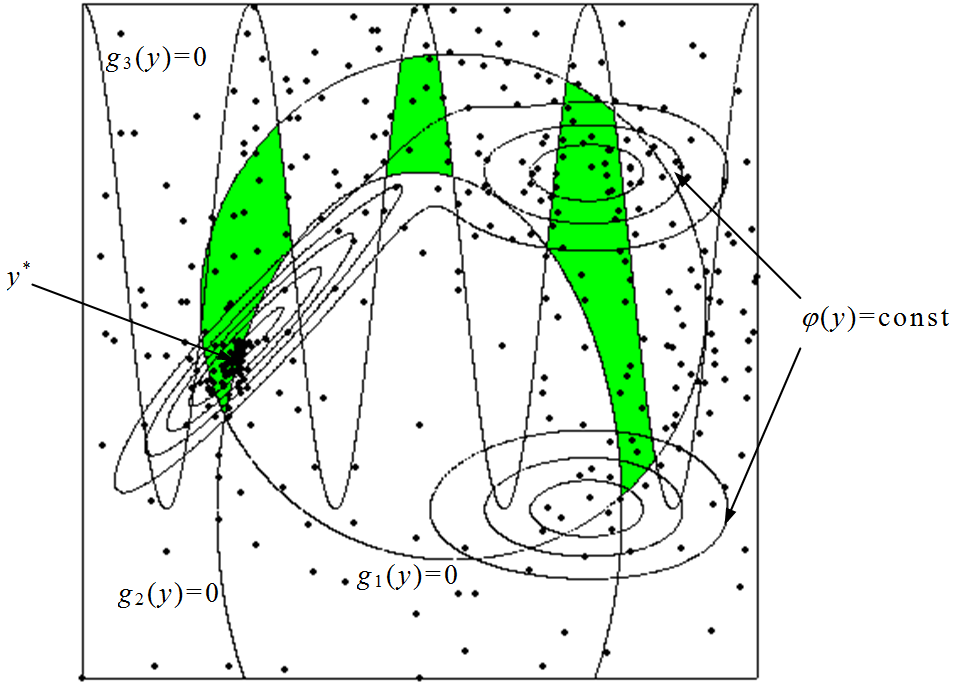
\includegraphics[width=0.8\linewidth]{figures/6_8.png}
\caption{The results of solving the problem using six processors}
\label{6_fig_8}     
\end{figure}
\end{example}

The results of the experiments (the number $k_i$ of computations of the values of the problem functions $g_i(y)$) are presented in tables \ref{6_tab2}--\ref{6_tab4}. Table~\ref{6_tab1} corresponding to the sequential algorithm is presented for comparison. 

\begin{table}
	\caption{The results of solving the problem on single processor}
	\label{6_tab1}
	\center
	\begin{tabular}{ccccc}
		\hline\noalign{\smallskip}
		$l$  & $k_1$ & $k_2$ & $k_3$ & $k_4$    \\
		\noalign{\smallskip} \hline \noalign{\smallskip}
		1 	&	1098 &	623 & 392	& 152 \\
		\noalign{\smallskip}\hline
	\end{tabular}
\end{table}

\begin{table}
	\caption{The results of solving the problem on two processors}
	\label{6_tab2}
	\center
	\begin{tabular}{cccccc}
		\hline\noalign{\smallskip}
		$l$  & $k_0$ &$k_1$ & $k_2$ & $k_3$ & $k_4$    \\
		\noalign{\smallskip} \hline \noalign{\smallskip}
		1 	&	636 &	567 & 331	& 212 & 104 \\
		2 	&	632 &	327 & 193	& 125 & 61 \\
		\noalign{\smallskip}\hline\noalign{\smallskip}
		Total 	&	1268 &	894 & 524	& 337 & 165 \\
		\noalign{\smallskip}\hline
	\end{tabular}
\end{table}

\begin{table}
	\caption{The results of solving the problem on four processors}
	\label{6_tab3}
	\center
	\begin{tabular}{cccccc}
		\hline\noalign{\smallskip}
		$l$  & $k_0$ &$k_1$ & $k_2$ & $k_3$ & $k_4$    \\
		\noalign{\smallskip} \hline \noalign{\smallskip}
1	&	585	&	508	&	311	&	206	&	88	\\
2	&	579	&	262	&	157	&	86	&	36	\\
3	&	579	&	293	&	174	&	119	&	41	\\
4	&	579	&	284	&	178	&	116	&	48	\\
		\noalign{\smallskip}\hline\noalign{\smallskip}
		Total	&	2322	&	1347	&	820	&	527	&	213 \\
		\noalign{\smallskip}\hline
	\end{tabular}
\end{table}

\begin{table}
	\caption{The results of solving the problem on six processors}
	\label{6_tab4}
	\center
	\begin{tabular}{cccccc}
		\hline\noalign{\smallskip}
		$l$  & $k_0$ &$k_1$ & $k_2$ & $k_3$ & $k_4$    \\
		\noalign{\smallskip} \hline \noalign{\smallskip}
1	&	354	&	289	&	165	&	105	&	44	\\
2	&	346	&	90	&	55	&	28	&	10	\\
3	&	346	&	113	&	66	&	40	&	10	\\
4	&	346	&	160	&	87	&	48	&	25	\\
5	&	346	&	224	&	119	&	68	&	23	\\
6	&	346	&	274	&	159	&	97	&	37	\\
		\noalign{\smallskip}\hline\noalign{\smallskip}
Total	&	2084	&	1150	&	651	&	386	&	149	\\
		\noalign{\smallskip}\hline
	\end{tabular}
\end{table}


The iteration speedup of the parallel algorithm on $p$ processors is presented in Table~\ref{6_tab5}. The iteration speedup was defined as the ratio of the number of iteration (which is equal to the number of checks of the first constraint $g_1$) executed by the sequential algorithm to the maximum number of iterations executed by the parallel algorithm on one of processors. This method of determining the speedup is important for the problems, in which the estimates of the functions' values requires considerable computational costs.

\begin{table}
	\caption{Iteration speedup of the parallel algorithm }
	\label{6_tab5}
	\center
	\begin{tabular}{cc}
		\hline\noalign{\smallskip}
		$p$  & speedup     \\
		\noalign{\smallskip} \hline \noalign{\smallskip}
		1 	&	--- \\
		2 	&	1.93 \\
		4 	&	2.16 \\
		6 	&	3.8 \\
		\noalign{\smallskip}\hline
	\end{tabular}
\end{table}

The results of the experiments clearly demonstrate the effect of speed up (the reduction in the number of the costly computations of the problem functions).

\section{Parallel computations based of novel schemes for building the multiple Peano curves}
\subsection{Scheme for building the rotated evolvents}

The application of the scheme for building the multiple evolvents (hereinafter called the shifted evolvents or $S$-evolvents) described in Subsection \ref{6_section_shift} allows to preserve the information on the nearness of the points in the multidimensional space and, therefore, to provide more precise (as compared to a single evolvent) estimate of Lipschitz constant in the search process. However, this approach has serious restrictions, which narrow the applicability of the parallel algorithms, designed on the base of the $S$-evolvents.

Because a shifted evolvent is built as a result of the shift of a hypercube $D$ along the main diagonal, and the shift step decreases 2 times for the building of each subsequent mapping, the number of such shifts is limited by the evolvent density $m$. In the case when the shift step is less than $2^{-m}$, the next evolvent coincides with the previous one. Thus, the applicable number of the evolvents $L$ and, hence, the number of processors are limited by $m$ ($L\leq m$), where $m$ is the density of the evolvents.

Also, it follows from the algorithm for building the shifted evolvents that solving the initial problem in the domain $D$ is reduced to solving a set of problems in the extended domains $D_l$ from (\ref{6_hypercubes}) with additional constraint (\ref{6_g0}). As a result, the structure of the search domain becomes more complicated, and the exponential decrease of the volume of the search domain $D$ in relation to the volumes of the domains $D_l$ with increasing dimensionality of the problem takes place.

To overcome the disadvantages mentioned above and to preserve the information on the nearness of the points in the $N$-dimensional space, a novel scheme of building of the multiple mappings is proposed. The building of a set of Peano curves not by the shift along the main diagonal of the hypercube but by rotation of the evolvents around the coordinate origin is a distinctive feature of the proposed scheme \cite{6_Gergel2009}. In the initial non-rotated mapping for close points $y', y''$ in the multidimensional space their preimages  $x', x''$ in the interval $[0,1]$ can be far away from each other. In the rotated scheme there exists a mapping $y^i(x)$ according to which preimages $x', x''$ will be located nearer. The evolvents generated according to the novel scheme will be hereinafter called the rotated evolvents or $R$-evolvents.

In Fig.~\ref{6_fig_9} two evolvents being the approximations to Peano curves for the case $N=2$ are presented as an illustration. The grid nodes in the $N$-dimensional space are marked by the dark dots. A pair of points, the preimages of which are far away from each other on the one-dimensional axis for one mapping and are close to each other for another mapping is pointed by the arrows. The maximum number of various rotations of the evolvents mapping the $N$-dimensional hypercube onto a one-dimensional interval is $2^N$. The employment of all possible rotations might appear to be redundant. In this case, one can select only a part of all rotations.

\begin{figure}[t]
%\sidecaption[t]
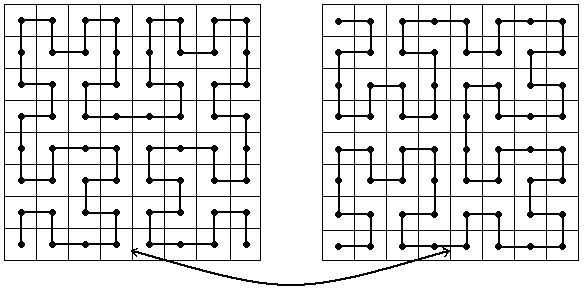
\includegraphics[width=0.8\linewidth]{figures/6_9.png}
\caption{Close/far points for the rotated evolvents}
\label{6_fig_9}     
\end{figure}

As a possible approach, one can propose to generate the new evolvents by the rotation of the initial evolvents on the angle of $\pm\pi/2$ in each of the coordinate planes. For example, the rotation matrices in the plane $(y_2,y_4)$ for  $N=5$ are presented below.
\begin{eqnarray*} 
 \begin{pmatrix}
  1 & 0 & 0 & 0 & 0 \\
  0 & 0 & 0 & -1 & 0 \\
  0 & 0 & 1 & 0 & 0 \\
  0 & 1 & 0 & 0 & 0 \\
  0 & 0 & 0 & 0 & 1
 \end{pmatrix}
\qquad \qquad
 \begin{pmatrix}
  1 & 0 & 0 & 0 & 0 \\
  0 & 0 & 0 & 1 & 0 \\
  0 & 0 & 1 & 0 & 0 \\
  0 & -1 & 0 & 0 & 0 \\
  0 & 0 & 0 & 0 & 1
 \end{pmatrix}
\end{eqnarray*} 

The number of such pairs of rotations is determined by the number of the coordinate planes in the space, which equals to  $N(N-1)/2$. The total number of the transformations equals to $N(N-1)$. Taking into account the initial mapping, one can conclude that this method allows to build up to $N(N-1)+1$ evolvents for mapping the $N$-dimensional domain onto the corresponding one-dimensional intervals. Moreover, the additional constraint  $g_0(y) \leq 0$ with $g_0(y)$ from (\ref{6_g0}), which arises in shifted evolvents, is absent. This method for building a set of mappings can be ``scaled'' easily to obtain more evolvents (up to $2^N$) if necessary.

The use of the set of mappings $Y_L(x)=\{y^1(x),...,y^L(x)\}$ results in the appearing of the corresponding set of the one-dimensional multiextremal problems 
\begin{equation}\label{6_problem_lr} 
\min{\left\{\varphi(y^l(x)):x\in [0,1], \; g_j(y^l(x))\leq 0, \; 1 \leq j \leq m\right\}}, \ 1 \leq l \leq L.
\end{equation} 
Each problem from this set can be solved independently. Any computation of the value $z=g_\nu(y'),\ y'=y^i(x')$ of the function $g_\nu(y)$ in the $i$-th problem can be interpreted as a computation of the value $z=g_\nu(y'),\ y'=y^s(x'')$ for any other $s$-th problem without time-comsuming computations of the functions $g_\nu(y)$. Such information integrity allows to solve  initial problem (\ref{6_problem}) by solving $L$ problems (\ref{6_problem_lr}) on a set of intervals $[0,1]$ in parallel by the index method. 

The decision rules for the parallel algorithm using $R$-evolvents coincide with the ones of the sequential algorithm almost completely except the method of the trial execution. Namely, the execution of a trial at the point $x^k \in [0,1]$ in the $s$-th problem in the case of using $R$-evolvents consists in the following sequence of operations.

\begin{enumerate}
	\item Determine the image $y^k=y^s(x^k)$ according to the mapping  $y^s(x)$.
	\item Inform the rest processors on the beginning of the trial execution at the point  $y^k$ (\textit{the blocking} of the point $y^k$).
	\item Compute the values $g_1(y^k),...,g_\nu(y^k),$ where the index $\nu \leq m$ are determined by the conditions
	\[
	g_j(y^k)\leq 0,\ 1\leq j< \nu,\ g_\nu(y^k) > 0,\ \nu \leq m.
	\]
	The first violation of the constraints terminates the trial at the point  $y^k$. In the case when $y^k$ is a feasible one, the trial includes the computation of all functions of the problem, and the index value is set to $\nu = m+1$. The triplet
	\begin{equation}\label{6_triplet_r} 
	y^s(x^k),\ \nu = \nu(x^k),\ z^k=g_\nu(y^s(x^k))
	\end{equation}
	is  \textit{the trial result} at the point $x^k$.
	\item Determine the preimages $x^{kl} \in [0,1],\; 1\leq l \leq L,$ of the point $y^k$ and interpret the trial executed at the point $y^k \in D$ as the execution of the trials in the $L$ points 
	\[
	x^{k1},...,\ x^{kL}
	\]
	with the same result 
	\[
	\nu(x^{k1})=...=\nu(x^{kL})=\nu(x^k),	
	\]
	\[
	g_\nu(y^1(x^{k1}))=...=g_\nu(y^L(x^{kL}))=z^k	
	\]
	and inform the rest processors on the results of the trial at the point $y^k$.		
\end{enumerate}

\subsection{Comparison of the algorithms}

\begin{example}

In order to compare the efficiency of the algorithms, the method of the operation characteristics has been applied. The series of experiments was devoted to minimixation of 100 two-dimensional functions of two variables
\begin{eqnarray} \label{6_VAG}
\varphi(y)= -&\left\{\left(\sum^{7}_{i=1}\sum^{7}_{j=1}A_{ij}g_{ij}(y)+B_{ij}h_{ij}(y)\right)^2+\right. \\
&\left.\left(\sum^{7}_{i=1}\sum^{7}_{j=1}C_{ij}g_{ij}(y)+D_{ij}h_{ij}(y)\right)^2\right\}^{1/2},\\ \nonumber
\end{eqnarray}
where
\begin{eqnarray} \nonumber
& y=(y_1,y_2)\in R^2, 0 \leq y_1,y_2 \leq 1, \\ \nonumber
& g_{ij}(y)=\sin(i\pi y_1)\sin(j\pi y_2),  \\ \nonumber
& h_{ij}(y)=\cos(i\pi y_1)\cos(j\pi y_2), \nonumber 
\end{eqnarray}
and coefficients $A_{ij}, B_{ij}, C_{ij}, D_{ij}$  are taken uniformly in the interval $[-1,1]$.

The experiments have been carried out for the algorithms described above with $S$-evolvents and $R$-evolvents  with the density $m = 12$. The number of evolvents $L = 2$, the parameters $r=2.1,\ \epsilon = 0.01$ and the reserves $\epsilon_\nu= 0.05$ from (\ref{6_z_nu}) have been used. These parameters are the minimal ones for the corresponding methods, for which the $100\%$ of the problems was solved. 

The operation characteristics of the methods obtained for the problem series generated according to (\ref{6_VAG}) are presented in Fig.~\ref{6_fig_11}. The lower dashed curve corresponds to the shifted evolvents method, the middle dashed one corresponds to the method with a single evolvent, and the upper solid curve corresponds to the rotated evolvents method. Such position of the curves demonstrates that the algorithm with $R$-evolvents provides in average faster obtaining the trial points falling into the predefined vicinity of the solution than the algorithm with $S$-evolvents  or the algorithm with a single evolvent.

\begin{figure}[t]
%\sidecaption[t]
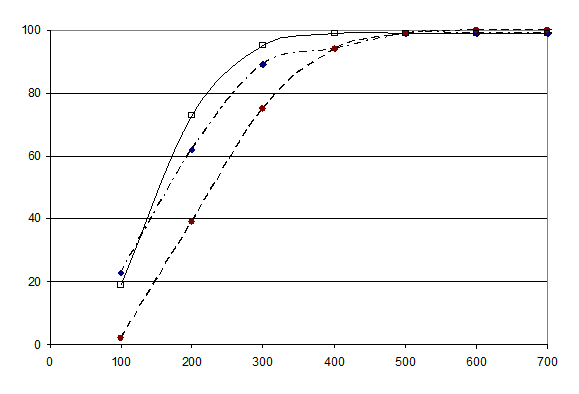
\includegraphics[width=0.8\linewidth]{figures/6_11.png}
\caption{The operation characteristics}
\label{6_fig_11}     
\end{figure}

\end{example}

\begin{example}
To illustrate the work of the parallel algorithm with $R$-evolvents for solving the essentially multidimensional problems, let us consider the minimization problem of the function
\[
\varphi(y) = \sum_{i=1}^N{\left(y_i^2-cos(18y_i^2)\right)},\ -1.5\leq y_i\leq 1.5, \ 1\leq i\leq N,\ N=6,
\]
where the minimum value $\varphi(y^\ast) = -N$ is achieved at the point $y^*=0$.

To solve this problem, the sequential method and the parallel one with the rotated evolvents with the density $m = 10$ were used. The parameter of the method $r=2.0$ and accuracy $\epsilon = 0.05$ in the termination criterion were employed. The number of evolvents $L = 30$ corresponds to the number of processors involved in solving the problem. The sequential algorithm as well as the parallel one have found the solution with the required precision; the sequential algorithm has executed 173116 iterations while the parallel one has executed 8535 (the maximum number of iterations for one processor). The iteration speedup was 20.28 and the time speedup was 7.48.
\end{example}

\begin{example}
Let us consider now the problem of minimization of the function from the previous example in the domain  $-1\leq y_i \leq 1,\ 1\leq i\leq N,$ for $N=15, 20$. In this experiment 100 processors were used. The speedup in time and the efficiency of finding the global optimum with respect to the number of trials with equal termination conditions were estimated. The results of solving the problems are presented in Table~\ref{6_tab_l1}.
	
	\begin{table}
	\caption{The results of multidimensional functions minimization}
	\label{6_tab_l1}
	\center
	\begin{tabular}{cccccccc}
		\hline\noalign{\smallskip}
		$N$ & $k$ & \multicolumn{2}{c}{ Sequential algorithm  } &\ & \multicolumn{3}{c}{Parallel algorithm } \\
		\noalign{\smallskip} \cline{3-4} \cline{6-8} \noalign{\smallskip}
		 & & Time & $\varphi_k^\ast$  &\  & Time & $\varphi_k^\ast$ & Speedup  \\
		\noalign{\smallskip} \hline \noalign{\smallskip}
%		11	&	$5\cdot10^6$	&	544068.8 & $-10.997$	& &	9321.5 & $-10.995$ 	&	112.01	\\
		15\	&	$3\cdot10^6$ \ &	605788 & $-14.835$	& &	7414 & $-14.925$ 	&	81.7	\\
		20\	&	$3\cdot10^6$ \ &	605956 & $-19.989$	& &	6654 & $-19.048$ 	&	91.06	\\
		\noalign{\smallskip}\hline
	\end{tabular}
\end{table}

It is clear from Table~\ref{6_tab_l1} that the index method with $R$-evolvents executed on 100 processors demonstrated the speedup close to the linear one with respect to the computational time that gives evidence its high efficiency.
\end{example}
\begin{example}
Now let us demonstrate the efficiency of the parallel index method in solving the constrained global optimization problem
\[
\varphi(y) = N + \sum_{i=1}^N{\left(y_i^2-\cos(2\pi y_i)\right)}\rightarrow\min 
\]
\[
g_1(y) = \sum_{i=1}^N{y_i} - 0.5 \leq 0
\]
\[
g_2(y) = \sum_{i=1}^N{y_i^2} - 1.0 \leq 0
\]
\[
g_3(y) = \sum_{i=1}^N{\sin(i\pi y_i)} - 0.3 \leq 0
\]
for $-1\leq y_i\leq 1,\ 1\leq i\leq N,\ N=8$. The results of solving this problem by the sequential method and by the parallel method on 56 processors are presented in Table~\ref{6_tab_l2}. In both cases, the methods terminated the search process upon achievement the predefined accuracy $\epsilon = 0.0035$. Table~\ref{6_tab_l2} shows number of trials $k$, number of objective function evaluations $k_4$, time of comutations $t$ in seconds, speedup in time $s$, iterations $S$ and in objective function evaluations $S_4$.
The maximum number of trials and objective function evaluations per one processor is specified in brackets.

	\begin{table}
	\caption{Comparison of the algorithms in solving a constrained problem}
	\label{6_tab_l2}
	\center
	\begin{tabular}{cccccccc}
		\hline\noalign{\smallskip}
		 Method & $k$ & $k_4$ & $S$ & $S_4$ & $t$ & $s$ & $\varphi_k^\ast$  \\
		\noalign{\smallskip} \hline \noalign{\smallskip}
		Sequential	&	309640 &	33874 & ---	& --- &	40006 & ---	&	0.016	\\
		Parallel	&	244356 (4891) \ &	22722 (789) & 63.3	& 42.9 &	626 & 63.8 	&	0.022	\\
		\noalign{\smallskip}\hline
	\end{tabular}
\end{table}

It is evident from Table~\ref{6_tab_l2} that the parallel algorithm demonstrated the speed up 63.3 with respect to the number of trials, 42.9 with respect to the number of objective function computations, and of 63.8 with respect to the computation time.
Note that the comparison of the sequential algorithm with the parallel one appears to be more difficult in the problems of higher dimensionality since in the latter case all the search information is concentrated in one computational node. There appeared to be not enough RAM for the sequential algorithm run on a single node. As a result, the swapping was activated. In the parallel algorithm, all data are distributed among the processors. This allows not to use the external memory for storing the search information.

\end{example}

\begin{thebibliography}{99.}

\bibitem{6_Sergeyev2006}
Sergeyev, Ya.D., Kvasov, D.E.: Global search based on efficient diagonal partitions and a set of Lipschitz constants. SIAM J. Optim. \textbf{16(3)}, 910--937 (2006)

\bibitem{6_Sergeyev2015}
Sergeyev, Ya.D., Kvasov, D.E.: A deterministic global optimization using smooth diagonal auxiliary functions. Communications in Nonlinear Science and Numerical Simulation. \textbf{21}, 99--111 (2015)

\bibitem{6_Sergeyev2017}
Sergeyev, Ya.D., Kvasov, D.E.: Deterministic global optimization: An introduction to the diagonal approach. Springer, New York (2017)

\bibitem{6_Zilinskas2008}
\v{Z}ilinskas, J.: Branch and bound with simplicial partitions for global optimization. Mathematical Modelling and Analysis \textbf{13(1)}, 145--159 (2008)

\bibitem{6_Zilinskas2014}
Paulavi\v{c}ius, R., \v{Z}ilinskas, J.: Simplicial Lipschitz optimization without the Lipschitz constant. J. Glob. Optim. \textbf{59(1)}, 23--40  (2014)

\bibitem{6_Zilinskas2014_1}
Paulavi\v{c}ius, R., \v{Z}ilinskas, J.: Simplicial Global Optimization. SpringerBriefs in Optimization, Springer, New York (2014)

\bibitem{6_Strongin2000}
Strongin, R.G., Sergeyev, Ya.D.: Global optimization with non-convex constraints. Sequential and parallel algorithms. Kluwer Academic Publishers, Dordrecht (2000)

\bibitem{6_Strongin2013}
Sergeyev, Ya.D., Strongin, R.G., Lera, D.: Introduction to Global Optimization Exploiting Space-Filling Curves. SpringerBriefs in Optimization, Springer, New York (2013)

\bibitem{6_Gourdin}
Gourdin, E., Jaumard, B., Ellaia, R.: Global optimization of H\"{o}lder functions. J. Global Optim. \textbf{8}, 323--348 (1996)

\bibitem{6_Lera2002}
Lera, D., Sergeyev, Y.D.: Global minimization algorithms for H\"{o}lder functions. BIT \textbf{42(1)}, 119--133 (2002)

\bibitem{6_Lera2010}
Lera, D., Sergeyev, Y.D.: Lipschitz and H\"{o}lder global optimization using space-filling curves. Appl. Numer. Math. 60(1–2), 115–129 (2010)

\bibitem{6_Hime}
e Oliveira, H.A., Petraglia, A.: Global optimization using space-filling curves and measure-preserving transformations. Soft Computing in Industrial Applications. \textbf{96}, 121--130 (2011)

\bibitem{6_Lera2015}
Lera, D., Sergeyev, Y.: Deterministic global optimization using space-filling curves and multiple estimates of Lipschitz and Hölder constants. Commun. Nonlinear Sci. Numer. Simul. \textbf{23}, 328--342 (2015)

\bibitem{6_Butz}
Butz, A.R.: Space filling curves and mathematical programming. Inform. Control \textbf{12(4)}, 314--330 (1968)

\bibitem{6_Sagan}
Sagan, H.: Space–Filling Curves. Springer–Verlag, New York (1994)

\bibitem{6_Strongin1991}
Strongin, R.G.: Parallel multi-extremal optimization using a set of evolvents. Comp. Math. Math. Phys. \textbf{31(8)}, 37--46 (1991)

\bibitem{6_Strongin1992}
Strongin, R.G.: Algorithms for multi-extremal mathematical programming problems employing the set of joint space-filling curves. J. Global Optim. \textbf{2(4)}, 357--378 (1992)

\bibitem{6_Gergel2009}
Strongin, R.G., Gergel, V.P., Barkalov, K.A.: Parallel methods for global optimization problem solving. Journal of instrument engineering. \textbf{52}, 25--33 (2009) (In Russian)

\end{thebibliography}

%\end{document}

%%%%%%%%%%%%%%%%%%%% author.tex %%%%%%%%%%%%%%%%%%%%%%%%%%%%%%%%%%%
%
%% sample root file for your "contribution" to a contributed volume
%
%% Use this file as a template for your own input.
%
%%%%%%%%%%%%%%%% Springer %%%%%%%%%%%%%%%%%%%%%%%%%%%%%%%%%%%%%%%%%
%
%
%%% RECOMMENDED %%%%%%%%%%%%%%%%%%%%%%%%%%%%%%%%%%%%%%%%%%%%%%%%%%%
%\documentclass[graybox]{svmult}
%%
%%% choose options for [] as required from the list
%%% in the Reference Guide
%%
%\usepackage{mathptmx}       % selects Times Roman as basic font
%\usepackage{helvet}         % selects Helvetica as sans-serif font
%\usepackage{courier}        % selects Courier as typewriter font
%%\usepackage{type1cm}        % activate if the above 3 fonts are
                             %% not available on your system
%%
%\usepackage{makeidx}         % allows index generation
%\usepackage{graphicx}        % standard LaTeX graphics tool
%%                             % when including figure files
%\usepackage{multicol}        % used for the two-column index
%\usepackage[bottom]{footmisc}% places footnotes at page bottom
%
%
%\usepackage[colorlinks=true]{hyperref}
%\hypersetup{urlcolor=blue, citecolor=blue}
%
%
%% see the list of further useful packages
%% in the Reference Guide
%
%\makeindex             % used for the subject index
                       %% please use the style svind.ist with
                       %% your makeindex program
%
%%%%%%%%%%%%%%%%%%%%%%%%%%%%%%%%%%%%%%%%%%%%%%%%%%%%%%%%%%%%%%%%%%%%%%%%%%%%%%%%%%%%%%%%%%
%
%\begin{document}

\title{Software systems for global optimization and the applied optimization problems}
\titlerunning{Software systems for global optimization } 

\author{Victor Gergel, Konstantin Barkalov, Alexander Sysoyev }
\authorrunning{V.Gergel, K. Barkalov, A. Sysoyev} 

\institute{Victor Gergel, Konstantin Barkalov, Alexander Sysoyev  \at Lobachevsky State University of Nizhni Novgorod,  Nizhni Novgorod, Russia \email{konstantin.barkalov@itmm.unn.ru}}
%
% Use the package "url.sty" to avoid
% problems with special characters
% used in your e-mail or web address
%
\maketitle

\abstract{This paper contains a description of the program systems for solving global optimization problems which have been developed by the authors. The first two systems -- GlobaLab and ParaLab -- are intended for educational and research goals and allow one to study both the known and new global search algorithms. These systems enable to realize the statement of an optimization problem, to choose a method of its solving, to execute a computational experiment and to analyze the results obtained. Such the capacities allow assimilating an experience in solving various global optimization problems, evaluating their efficiency and getting necessary knowledge and skills. After the study of the theory and practical training in optimization on the base of the abovementioned systems the reader can get acquainted with the GlobalExpert system that provides the possibility of solving complicated optimization problems arising in different areas of applications. The examples of solving the applied problems in the fields of optimal design, chemical research and economics are given.}


\section{The software system GlobaLab for investigation and study of global optimization methods}

Globalizer Laboratory (\textit{GlobaLab}) is an integrated software system for carrying out the experiments with the global search methods for study and investigation of the basic concepts, approaches, and the algorithms in the field of \textbf{global optimization}.

The multiextremal optimization problems considered within the framework of the theory of global search are the subject of extensive studies and are applied widely in computer aided design, in solving the identification problems, etc. GlobaLab belongs to the class of systems for carrying out the computational experiments, the development of which is an important area of the novel research techniques in various fields of science and technologies.

The availability of all necessary tools for carrying out the computational experiments is a distinguishing feature of the system. Using GlobaLab, the user of the system (\textit{the optimizer}) can formulate the statement of an optimization problem, select the optimizing algorithm from the list of the global search methods available in the system, set up the graphic indicators for monitoring the global search process, carry out various computational experiments, obtain and analyze the experiment results. These completeness and orientation on the novel technologies of education distinguish GlobaLab from other systems (such as, for example, SYMOP \cite{7_Gergel1993} and LGO \cite{7_Pinter1996}).

The possible fields of application of the system are:
\begin{itemize}
\item \textit{education}: applying by the students and teachers for their investigations and study of the global search methods within the framework of the laboratory training for various disciplines of the optimization oriented curriculum (optimization methods, system analysis, operations research, etc.). GlobaLab can be used for demonstrations of a number of important concepts of mathematics and computer science (sequences, limit points, convergence of a numerical method, etc.). GlobaLab can also be used as an example of a complex approach to the development of the computer simulation systems;

\item \textit{research}: applying by the researchers in the fields of the multiextremal optimization theory for the investigations of the efficiency of the global search algorithms under development. The system can be used as a tool for preparing and carrying out the scientific demonstrations of numerical solving the optimization problems by various methods;

\item \textit{applications}: applying by the experts and researchers as a training component of the complex professional optimization systems.
\end{itemize}

\begin{figure}[t]
%\sidecaption[t]
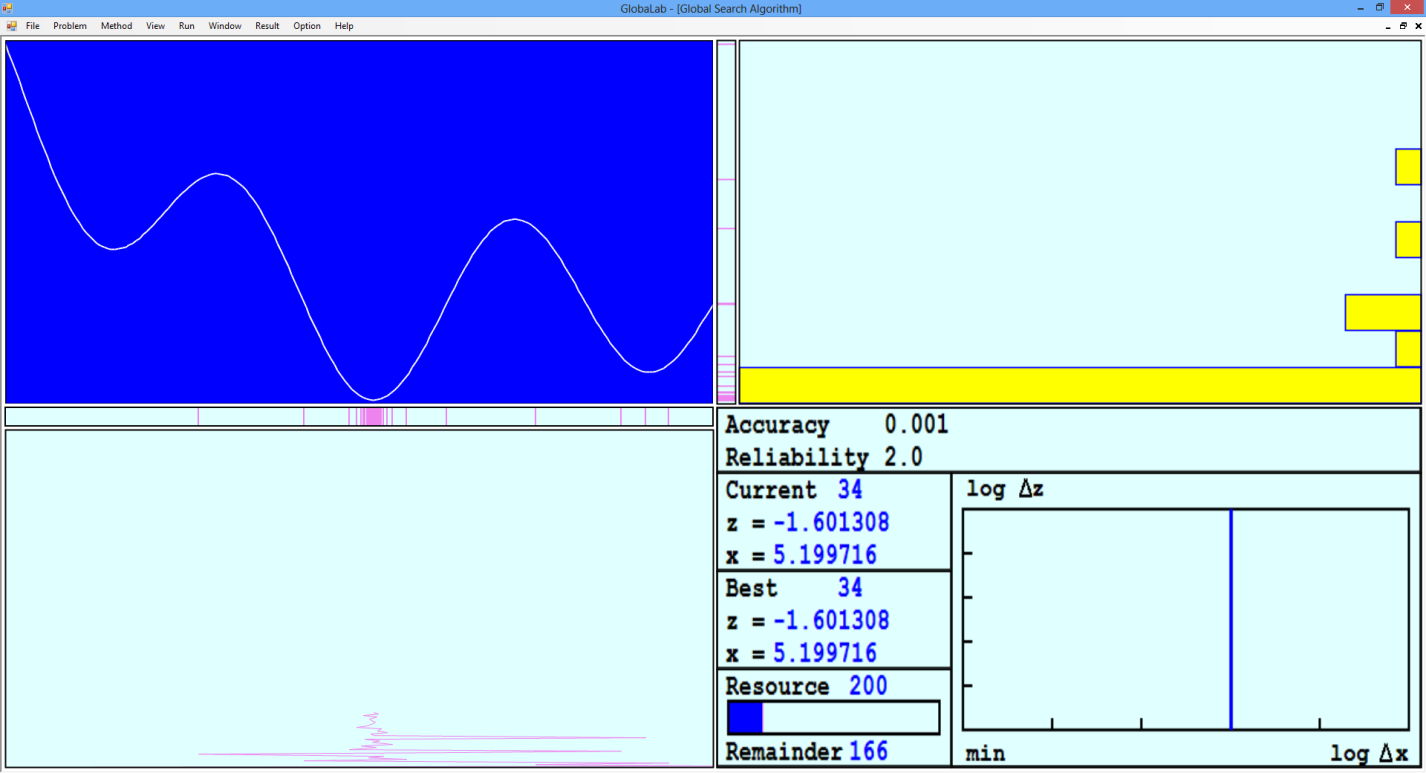
\includegraphics[width=1.0\linewidth]{figures/7_1.png}
\caption{GlobaLab main window}
\label{7_fig_1}     
\end{figure}

The users beginning to study the global search problems can find GlobaLab to be useful to get acquainted with the multiextremal optimization methods. The experienced optimizers can use the system to estimate the efficiencies of newly developed global search algorithms. A screenshot of the GlobaLab main window is presented in Fig.~\ref{7_fig_1}.

\textbf{Capacities of the system.} GlobaLab is an integrated program environment for carrying out the experiments with the global search methods. The user of the system is allowed:

\begin{itemize}
\item \textit{to formulate the statement of the optimization problem}. The minimized function can be selected from a list of the standard functions, generated by a random generator, defined by a formula, or formed by a graphic editor;

\item \textit{to select a global search algorithm} from the list of the optimization methods implemented in the system. GlobaLab supports 10 various multiextremal algorithms, the most known in the theory and practice of the global search. The system provides a possibility to extend the set of methods by the build-in tools without using the algorithmic programming languages;

\item \textit{to set up the graphic indicators} for monitoring the global search process; these indicators allow visualizing the graph of the minimized function or its piecewise linear approximation, the distribution, density, and sequence of the iteration points and of the function values at these points. Monitoring the indicators in the global search process provides better understanding of the global optimization theory and develops the intuition necessary for the practical application and further development of the multiextremal optimization methods;

\item \textit{to carry out various computational experiments} sequentially or in parallel. The latter case allows visual comparing the search dynamics by various methods and is realized in the time sharing mode. Carrying out the series of computational experiments requiring long computation times can be performed automatically with the option of storing the search results for further analysis of the data obtained. Executing the numerical experiments can be performed in the manual mode as well, when the optimizer indicates the iteration points manually (this mode allows the user to verify various hypotheses, which can serve as the base for the development of novel global search methods);

\item \textit{to accumulate and analyze the results of the computational experiments}. GlobaLab allows estimating the operation characteristics of the methods and provides the logging of the experiments in order to record the results of the optimization. The accumulated data can be presented in various generalized forms (tables, graphs, charts) convenient for further analysis. The results of the computations can be stored in a system archive, printed out, or copied to the Windows as text, graphics, or table and transferred to Word, Excel, or another Windows application programs for further processing and analysis (including for the use in preparing the scientific publications, reports, etc.).
\end{itemize}


\section{The software system ParaLab for studying and investigation of the parallel computation methods}

Parallel Laboratory (\textit{ParaLab}) is a software system that provides the possibility to carry out the computational experiments with the purpose of studying and investigation of the parallel algorithms for solving complex computational problems. The system can be used in the laboratory training in various training courses in the field of parallel programming, within which the following possibilities are provided:

\begin{itemize}
\item \textit{the modeling of the parallel multiprocessor computation systems} with different topologies of the networks for the data transfer; 

\item \textit{the visualization} of the computational processes and of the data transfer operations at the parallel solving of different computational problems; 

\item \textit{the estimation of the efficiency} of the parallel computation methods studied.
\end{itemize}

The conduction of such training can be organized on the «ordinary» single processor computers running under the operation systems of MS Windows family (the multiprocess parallel computations simulation mode). Besides the simulation mode, ParaLab can provide the remote access to a multiprocessor computational system for carrying out the numerical experiments in the «true» parallel computations mode in order to compare the results of simulation with the ones of real parallel computations.

In general, ParaLab system is an integrated computational environment for studying and investigation of the parallel algorithms for solving complex computational problems. A wide choice of available tools for the visualization of the computational experiment execution process and for the analysis of the obtained results allows studying the efficiency of application of various algorithms using various computational systems, to make the conclusions on the scalability of the algorithms, and to determine possible speedup for the parallel computation processes.

The educational and research capabilities provided by ParaLab are directed onto the active learning of the theoretical basics and methods, onto encouraging the students to develop their own ideas on the models and methods of the parallel computations by visualization, comparison, and analysis of large set of various graphic indicators and viewers, activated during the experiments.

The main application area of the system is the application in education by the students and teachers for the investigation and studying the parallel algorithms for solving the complex computational problems within the framework of the laboratory practicum in various training courses in the field of parallel programming. ParaLab system can be used also in carrying out research for the estimation of the parallel computations. The users, beginning to study the problems of parallel computing will find ParaLab system to be useful in learning the methods of parallel programming. The experienced programmers can use the system to estimate the efficiency of newly developed parallel algorithms.
A screenshot of the main window of ParaLab system, which a test optimization problem was run in, is presented in Fig.~\ref{7_fig_2}).

\textbf{Capacities of the system.} ParaLab is a software system, which allows conducting the real parallel computations on a multiprocessor computational system as well as the simulations of such experiments on a single serial computer with the visualization of the process of the parallel solving a complex computational problem.

In carrying out the simulation experiments, ParaLab provides the following possibilities for the users:

\begin{itemize}
\item \textit{to define the topology} of the parallel computational system for carrying out the experiments, to define the number of processors in this topology, to set the performance of the processors, to select the parameters of the communication environment and the communication method;

\item \textit{to formulate the statement of the computational problems}, for which in the system there are the built-in parallel algorithms to solve it, to set the parameters of the problem;

\item \textit{to select a parallel method} for solving the specified problem;

\item \textit{to set the visualization parameters} to choose the desired rate of the demonstration, the displaying method for the data transferred between the processors, and the level of the visualization details in the parallel computations;

\item \textit{to carry out the computational experiments} on the parallel solving the specified problem; several different \textit{computational experiments} can be formed in ParaLab with different types of multiprocessor systems, problems, or parallel methods, which the experiments can be run in parallel (in the time sharing mode); the parallel execution of several experiments allows to compare the dynamics of the problem solving by various methods using various topologies with various parameters of the studied problem. If a series of experiments is executed requiring long-time computations, the system provides a possibility to execute the experiments in an automatic mode with saving the numerical results for further analysis of the obtained data,

\item \textit{to accumulate and analyze the results of the experiments}; the system provides the tools for visualizing the saved data featuring the parallel computations (computation time, speedup, efficiency) as the functions of the parameters of the problem and of the computational system.
\end{itemize}

\begin{figure}[t]
%\sidecaption[t]
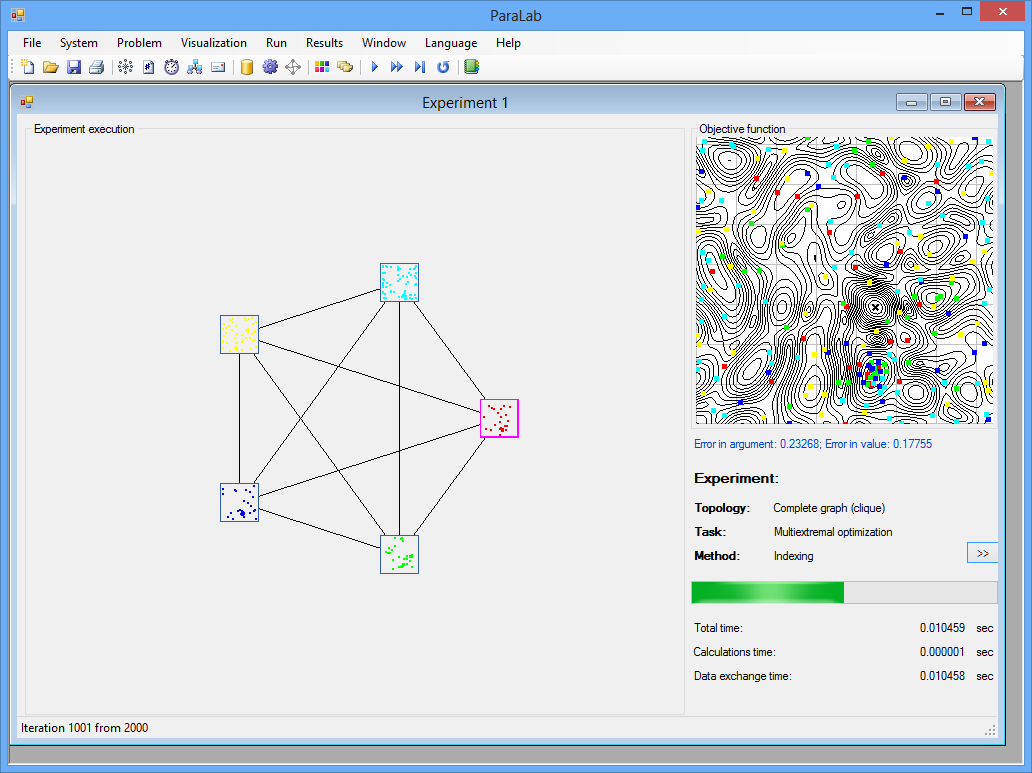
\includegraphics[width=1.0\linewidth]{figures/7_2.png}
\caption{ParaLab main system (global optimization problem is selected)}
\label{7_fig_2}     
\end{figure}

The possibility to choose the method of carrying out the experiments is one of the most important features of ParaLab. The experiments could be performed \textit{in the simulation mode}, i.e., performed on a single processor without using any parallel specialized software like the message transfer libraries. Besides, ParaLab provides the possibility to carry out \textit{the real computational experiments on parallel computers}.

In visualizing the dependencies of the time characteristics on the parameters of the problem and of the computational system for the experiments carried out in the simulation mode the theoretical estimates are used according to the available models of the parallel computations. For the real computational experiments on the multiprocessor computer systems, the dependencies are visualized according to the results of the real numerical experiments. 

It is worth noting that ParaLab provides storing the results of the executed experiments in a special memory buffer. The stored results allow performing the analysis of the obtained data. Any experiment executed earlier can be restored to be recomputed again or to continue the computations according to pre-stored information. 

The education and research processes realized in this way allow getting acquainted with the theoretical basis and assist to develop the methods of design of the parallel algorithms aimed at solving time-consuming applied problems. More detailed information on the ParaLab system is presented in \cite{7_Gergel2010}.


\section{The software system GlobalExpert for parallel solving the global optimization problems}

GlobalExpert is an integrated software for solving the global optimization problems using the parallel computational architectures. This system has been developed on the base of the information-statistical theory of multiextremal optimization in the framework of which many efficient parallel global search algorithms have been designed [ ].

Using GlobalExpert, the researchers can formulate the statement of the optimization problem, select an optimization algorithm from the list of the global search methods build-in in the system, set up the graphic indicators for monitoring the global search process, to execute the computations, obtain and analyze the results. 

GlobalExpert is oriented to the application by the engineers and researchers as an efficient tool for solving the multidimensional global optimization problems. 
A considerable time of the computation of the optimized function at single point, which may reach tens of seconds is a key characteristic of the applied problems. In this case to solve optimization problems in a reasonable time GlobalExpert accumulates and analyzes scrupulously all optimization data computed in the search process. 

The system consists of two main parts: the optimization subsystem and the management one. The management subsystem is implemented as a .NET application using the managed C++ programming language. It is designed for the control of the computations and for displaying the calculated results. Using the management subsystem, the researchers get the following possibilities:

\begin{itemize}
\item \textit{to form an optimization problem} (to define the functions, to select the criteria and constraints, to define the feasible domain for the variables);

\item \textit{to perform a preliminary investigation of the problem} (to plot the function sections and/or the level lines of the problem functions, to analyze the feasible domain of the problem fixing some variables);

\item \textit{to select the optimization method} and to set its parameters;

\item \textit{to select the running mode for the executive module} (serial, parallel on a single computer, parallel in a multiprocessor system);

\item \textit{to monitor the search process in real time};

\item \textit{to modify the problem statement and/or the method parameters} and to solve the problem in a new statement using the search information accumulated earlier.
\end{itemize}

A screenshot of the main window of the management subsystem is presented in Fig.~\ref{7_fig_3}).

\begin{figure}[t]
%\sidecaption[t]
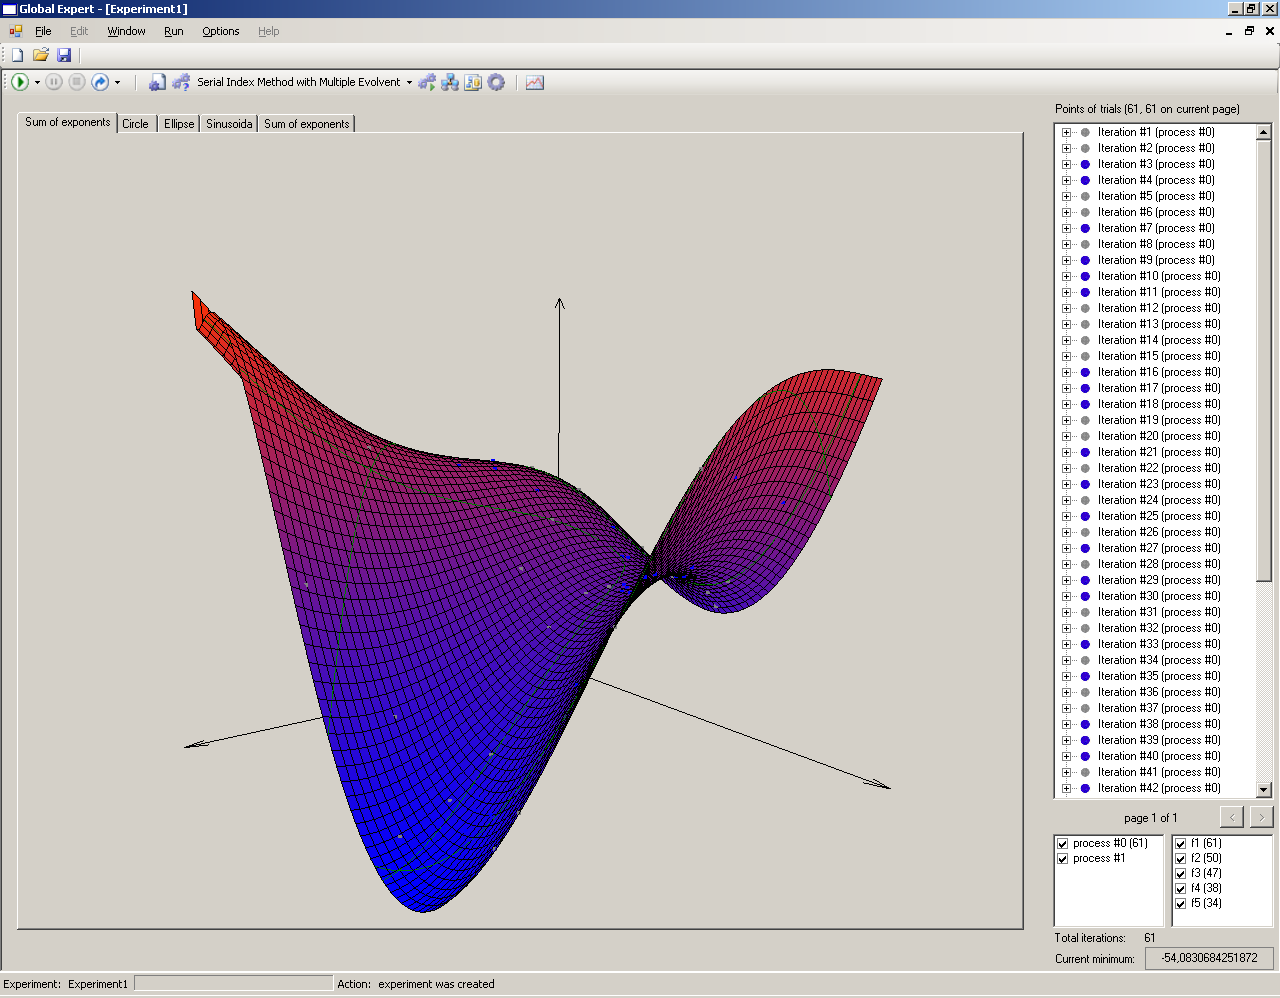
\includegraphics[width=1.0\linewidth]{figures/7_3.png}
\caption{Modeling of the wheel profile}
\label{7_fig_3}     
\end{figure}

The optimization subsystem is implemented in the form of an executable file as well as a module of a dynamic library (developed using С++ programming). In the form of the dynamic library module it can be linked to an application software system as a «solver» for the optimization problems. In the form of the executable file this module can be run either independently (the results are displayed in the console window) or under control of the management subsystem (the results are transferred to the management subsystem for visualizing and processing). 

When performing a large amount of computations the following procedure is recommended for solving time consuming optimization problems. First, one has to perform a preliminary calculations using the management subsystem, to ensure the correct problem statement and correctness of the results obtained when running the problem on a single computer or on a parallel computer with several processors. To run the computations on a real multiprocessor high-performance system, one has to run the executable file of GlobalExpert via the job management of the computational system. With this purpose, the generation of the command line with all options required for running a job on the parallel computer is provided in the management subsystem.

Capacities of the system. GlobalExpert is an integrated program environment for solving the global optimization problems. It allows: 

\begin{itemize}
\item \textit{to modify the statement of the problem} being solved without the loss of the accumulated search information (modification of the constraints set, change of the minimized function, expanding/reducing the search domain);

\item \textit{to use a number of the information global search algorithms} (GlobalExpert includes several serial and parallel algorithms, which demonstrated the high efficiency performance in various applications);

\item \textit{to display the visual information} on the problem being solved in the user-friendly form. The researcher can plot various sections of the problem functions, display the level lines of the minimized functions, the distribution of the iteration points on the function graphs and/or on the level lines, select the iteration points from different processors, etc. 

\item \textit{to accumulate and analyze the results} of the executed experiments. GlobalExpert provides logging of the executed experiments for storing the optimization results. The results of the computations include the search data from all processors, which the system has been run on. The accumulated data are presented in the tabular form, which is convenient for analysis and further processing. 
\end{itemize}



\section{Optimization of the rail transport wheel profile}

The considered problem of the search for the optimum profile of the wheels for the rail transport (railway, subway, tram, etc.) has been solved in the framework of joint research project supported by Russian Foundation for Basic Research (project number 04-01-89002-NVO\_a) and NWO (Netherlands Organization for Scientific Research, project number 047.016.014)  ``Fast Computing in Global Optimization: Sequential and Parallel Environments'', carried out at Lobachevsky State University of Nizhni Novgorod and Delft University of Technology, the Netherlands (TU Delft).

\subsection{Problem Statement}

The problem of the rail transport wheel profile optimization is described in details in \cite{8_Markine2005,8_Markine2007}. Here, a brief description of this problem is presented only. Since the wheels are of the conical shape, the center of a mounted axle is moving along a sinusoid. This process is illustrated in Fig.~\ref{8_fig_1}). The parameters of the contact between the wheel and the rail, such as the radius of rotation, the contact angle, and the angle of inclination for the mounted axle are varied at the transverse displacement of the mounted axle relative to the rail. The relationship between these variations and the transverse position of the mounted axle is determined by the wheel and rail profiles.

\begin{figure}[t]
%\sidecaption[t]
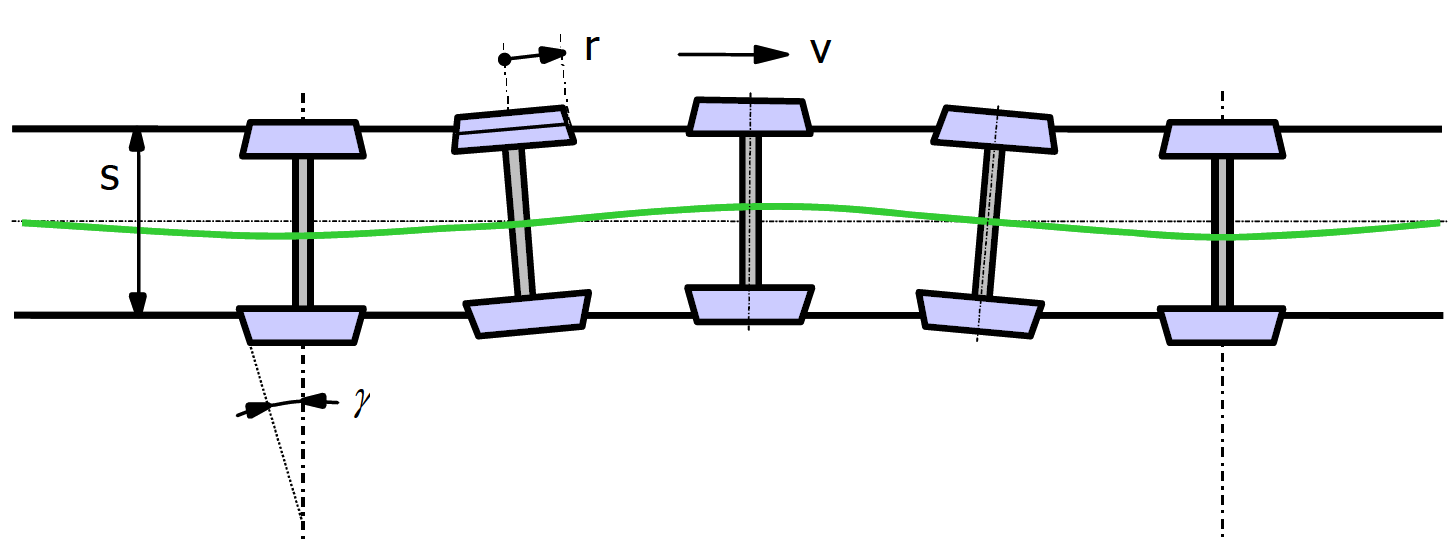
\includegraphics[width=0.9\linewidth]{figures/8_1.png}
\caption{The displacement of the mounted axle}
\label{8_fig_1}     
\end{figure}

The radius of rotation of the wheel at the contact point is an important parameter of the contact between the wheel and the rail. Actually, the radius can be different for the right and the left wheels since the mounted axle can shift relative to the rail (the radii $r_1$ and $r_2$, respectively in Fig.~\ref{8_fig_2}).

\begin{figure}[t]
%\sidecaption[t]
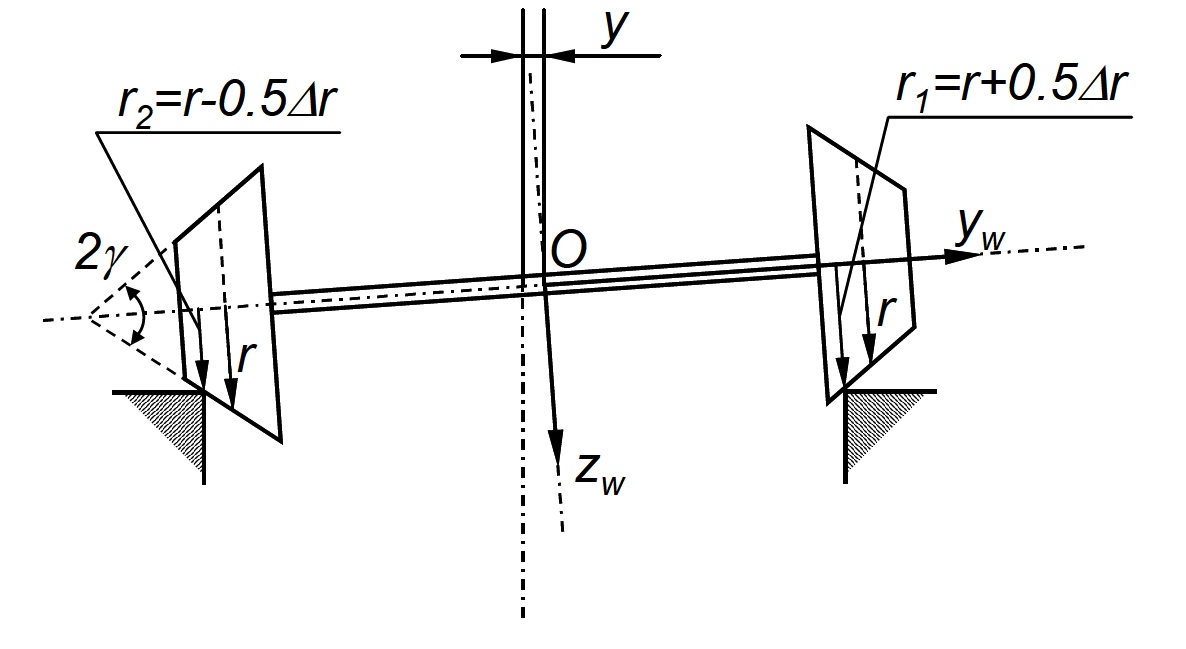
\includegraphics[width=0.7\linewidth]{figures/8_2.png}
\caption{The difference in the radii of rotation}
\label{8_fig_2}     
\end{figure}

When the mounted axle is in the central position, the radii of rotation are the same for the left and right wheels, i.e., $r_1=r_2=r$. The difference in the radii of rotation for the left and right wheels can be defined as a function of the transverse displacement of the mounted axle relative to its central position $\Delta r(x)=r_1(x)-r_2(x)$.

The mathematical model for this problem developed in Technical University Delft consists in the following. The wheel profile is described by B-spline, for building of which a set of points on the edge, on the edge base, and on the rolling surface of the wheel were selected (Fig.~\ref{8_fig_3})). Positions of these points can be varied for the purpose of variation of the profile. In order to reduce the computational costs for the optimization, the positions of the points on the upper surface of the edge as well as on the conical part of the profile were fixed since these parts of the wheel profile do not contact the rails.

\begin{figure}[t]
%\sidecaption[t]
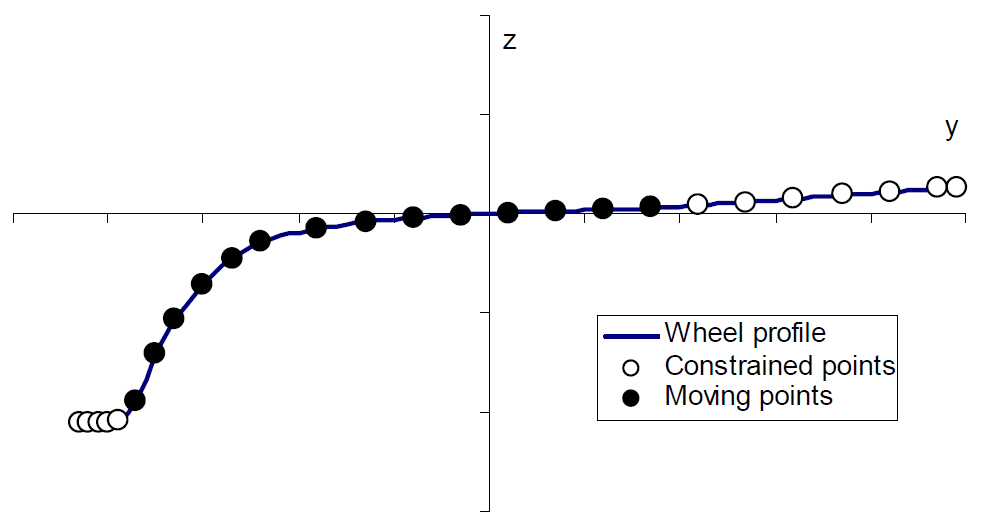
\includegraphics[width=0.7\linewidth]{figures/8_3.png}
\caption{Modeling of the wheel profile}
\label{8_fig_3}     
\end{figure}

The ordinates of the movable points of the spline $z_i$ were selected as the components of the vector of the optimization problem parameters $y$, i.e.,
\[
y=(z_1,...,z_N),
\]
and the abscissas of these points were fixed.

The number of the movable points and, consequently, the number $N$ of variables in the considered problem was equal to $11$. For each parameter   the interval $\left[–1, 1\right]$ was taken as the domain of its variation. The difference of the radii of rotation $\Delta r(x)$ was minimized. The constraints were introduced according to the stability considerations. For example, one of the constraints was imposed on the maximum angle of inclination for the mounted axle.

\subsection{The results of the experiments}

Thus, the optimization problem has $N=11$ parameters and $m=6$ constraints. The objective function as well as the constraint functions is the multiextremal ones. A one-dimensional section of the objective function is presented in Fig.~\ref{8_fig_4} for illustration.

\begin{figure}[t]
%\sidecaption[t]
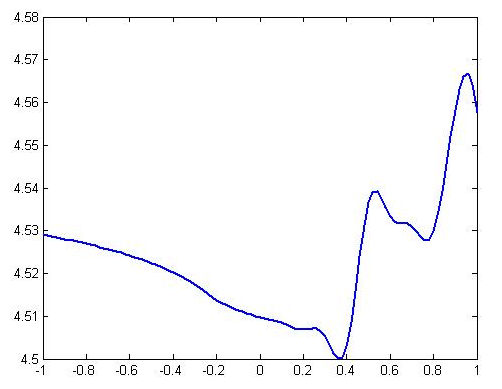
\includegraphics[width=0.7\linewidth]{figures/8_4.png}
\caption{A section of the objective function }
\label{8_fig_4}     
\end{figure}

The constraints have no analytical form and defined by a MATLAB computational procedures. The computation of the values of all problem functions (objective function and constraints) at one point $y$ using Pentium IV processor with the clock frequency of 3 GHz takes about 10 sec. 

Thus, having formulated the problem, let us try to estimate the resources required for its solving in dependence on the method selected. Let us take, for example, the method of full scanning a uniform grid. Having selected 10 variants for the values of each parameter (remind, that the total number of parameters equals to 11), we obtain $10^{11}$ computations at the grid nodes that requires $\sim 10^{12}$ sec., i.e., $\sim 3$ years of computations using a supercomputer with 10 000 processors. Thus, the problem is so hard to solve that the parallel computations are not only necessary but should be supplied with the efficient numerical methods to obtain the results in a reasonable time unavoidably.

The problem described above has been solved by the authors using the parallel index method with the multiple shifted evolvents on a cluster of 4 computers in Delft University of Technology. The search precision in the coordinates was $2^{-10}$ , i.e., 1024 points of each parameter value in the case of the full scanning method. The search time for the optimum estimate was 27 hours. The problem functions values have been computed $4297 + 4415 + 4236 + 4266 = 17214$ times.

The computations carried out at TU Delft for a wheel of the optimum profile demonstrated its service life to increase up to 120 000 km between the profile corrections (more than five times longer as compared to the wheels of the original profile) and the maximum permitted speed to increase from 40 up to 60 m/sec.

\section{Solving the inverse problem of chemical kinetics}

In the present section the results of joint research project carried out at Lobachevsky State University of Nizhni Novgorod and at Institute of Petrochemistry and Catalysis, Russian Academy of Sciences (IPC RAS) \cite{8_Gubaidullin2011}.

\subsection{Problem statement}

The building of the mathematical models of the complex chemical reactions implies the presence of the unknown kinetic parameters (the rate constants, the activation energies, and the frequencies of collisions between the reacting molecules), which could be found by solving the problem of the minimization of the deviations between the calculated data (\textit{the direct problem}) and the experimental ones. Thus, a problem of identifying the mathematical model (\textit{the inverse problem of chemical kinetics}) arises, which in general case is a global optimization problem.

Many problems of physics chemistry imply a considerable amount of computations, nevertheless, providing rather low precision. Investigating the inverse problems of chemical kinetics requires solving many systems of differential and algebraic equations. The kinetics of complex chemical reactions is featured by the presence of parameters varying fast and slowly (because various stages of reactions go with different rates). Therefore, solving the direct kinetic problems is complicated by the hardness of the differential equations describing the mechanisms of these reactions.

The direct kinetic problem for the isothermal non-stationary model in a closed system is Cauchy problem for a system of ordinary differential equations
\begin{equation} 
 \frac{dx_i}{dt}= F_i, i=1,..,M; \; F_i=\sum_{j=1}^{N}{S_{ij}w_j}
\end{equation}
\begin{equation} 
 w_j=k_j\prod_{i=1}^{M}{\left(x_i\right)^{\left|\alpha_{ij}\right|}}-k_{-j}\prod_{i=1}^{M}{\left(x_i\right)^{\left|\beta_{ij}\right|}}
\end{equation}
with the initial conditions $t=0$, $x_i(0)=x_i^0$, where 
\begin{itemize}
	\item $x_i$ are the concentrations of the substances (\textit{the molar fractions}) participating in the reaction;
	\item $M$ is the number of substances; 
	\item $N$ is the number of steps;
	\item $S_{ij}$ are the stoichiometric matrix; 
	\item $w_j$ are the rates of the $j$-th step, $1/{hr}$; 
	\item $k_j$, $k_{-j}$ are the reduced rate constants for the forward and reverse reactions ($1/{hr}$), respectively;
	\item $\alpha_{ij}$ are the negative elements of $S_{ij}$, and $\beta_{ij}$ are the positive elements of $S_{ij}$.
\end{itemize}

Since a part of the constants $k_j$, $k_{-j}$, as a rule, are not known, the problem of identification of the mathematical model of  the inverse kinetic problem arises. This problem is a minimization one for the function of the deviation between the calculated data and the experimental ones
\begin{equation} \label{8_chem_func}
F=\sum_{i=1}^n{\sum_{j=1}^M{\left|x_{ij}^p-x_{ij}^{\epsilon}\right|}}\rightarrow \min,
\end{equation}
where
\begin{itemize}
	\item $x_{ij}^p$ are the calculated values of the observable substances concentrations  (\textit{molar fractions});	
	\item $x_{ij}^{\epsilon}$ are the values of the observable substances concentrations measured experimentally (\textit{molar fractions});
	\item $n$ is the number of the experimental points.
\end{itemize}

To find the activation energies and the collision frequencies of the molecules reacting at the elementary step, Arrhenius equation
\[
k=Ae^{-\frac{Ea}{RT}}
\]
is used, where
\begin{itemize}
	\item $k$ is the reduced rate constant for the elementary step, $1/hr$;	
	\item $E$ is the activation energy, $J/{mol}$;
	\item $R$ is gas constant, $J/{(mol \cdot K)}$;
	\item $А$ is the collision frequency for the reacting molecules;
	\item $T$ is the temperature, $K$.	
\end{itemize}

Since in the search for the rate constants of the elementary steps, these ones may fall into the area, where the differential equations system describing the reactions may appear to be a stiff one, Mishelsen method with automatic step selection is applied to solving the direct problem \cite{8_Gubaidullin2010}. As the model output data $x_{ij}^p$ depend on the values of the constants $k_j$, $k_{-j}$ nonlinearly, problem (\ref{8_chem_func}) is a multiextremal optimization problem.

\subsection{The results of the experiments}

Traditionally, the methods based on the random search ideas had been applied in IPC RAS for solving problem (\ref{8_chem_func}). The typical computation costs were several days of continuous computations. Within the framework of the joint research project by IPC RAS and Lobachevsky State University of Nizhni Novgorod it was proposed to apply the efficient parallel global optimization methods developed in UNN. 

For the application of the novel identification technique the mathematical model for the reaction of the catalytical carboalumination of olefins and acetylenes with the assistance of threealkylalanes in the presence of transition metal complexes was selected. This reaction has applied in the laboratory research at IPC RAS as an efficient method for the synthesis of new Me-C (methyl-carbon), Et-C (ethyl-carbon), and C-C (carbon-carbon) bonds \cite{8_Parfenova2009}. The natural experiments of conducting the reactions of the catalytical carboalumination of olefins and acetylenes for different temperatures and fixed initial concentrations have been carried out in IPC RAS. In the experiments, the concentrations of five substances were traced and their percentage ratios were determined. A number of schemes for the mathematical description of the reaction of catalytical carboalumination of olefins and acetylenes (including the parameters to be identified) have been proposed in IPC RAS. As a priority problem of the identification of the unknown parameters, it was required to determine the rate constants for the elementary steps for the proposed reaction schemes for various temperatures as well as to find the activation energies for the elementary steps for various catalysts. These schemes and the identification problem have been described in details in \cite{8_Gubaidullin2011}. Here, note that the minimization problem arising depends on 10 parameters and is box-constrained one. The computational costs for the function value at one point are $\sim 3$ sec. (Intel Xeon 3.2 GHz). The objective function is  multiextremal that is confirmed by its two-dimensional section presented in Fig.~\ref{8_fig_5}. 

\begin{figure}[t]
%\sidecaption[t]
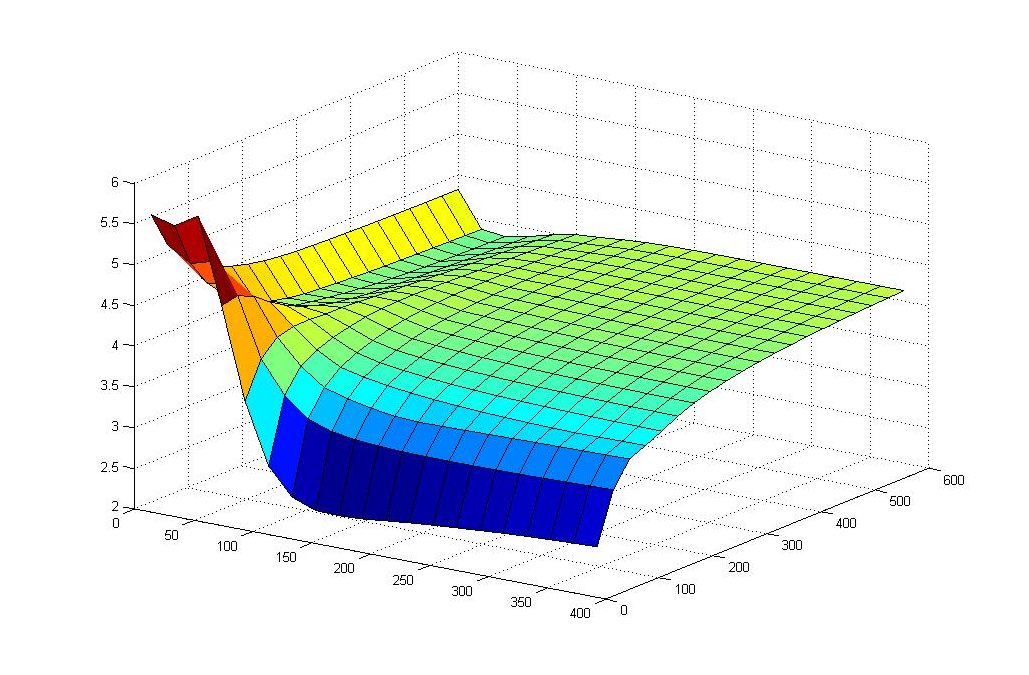
\includegraphics[width=0.8\linewidth]{figures/8_5.png}
\caption{Two-dimensional section of the objective function}
\label{8_fig_5}     
\end{figure}

As a result of the computations, the estimates of the rate constants for the elementary steps for the 10- and 12-step reactions schemes of the carboalumination in the presence of $Cp_2 ZrCl_2$ catalyst have been obtained. The objective function value at the obtained optimizer was $F = 3.040$. It appeared to be impossible to achieve the function value close to zero because the experimental data contains the uncertainties. Nevertheless, the model identified using the parallel global optimization method allowed obtaining a good conformity between the calculated data and the experimental ones. As an illustration, the comparison of the computed and experimental concentrations of substances participating in the reactions is presented in Fig.~\ref{8_fig_6}.

\begin{figure}
\begin{minipage}{0.5\linewidth}
\center{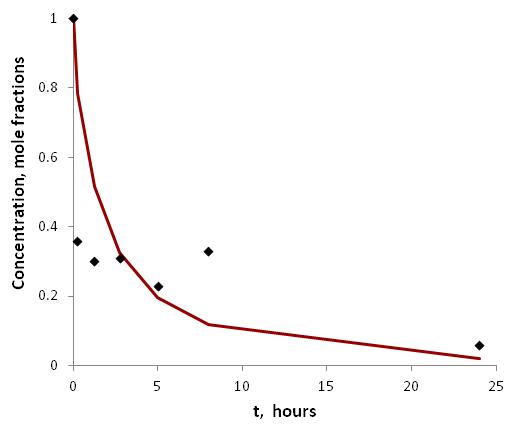
\includegraphics[width=1.0\linewidth]{figures/8_6a.png} \\ (a)}
\end{minipage}
\hfill
\begin{minipage}{0.5\linewidth}
\center{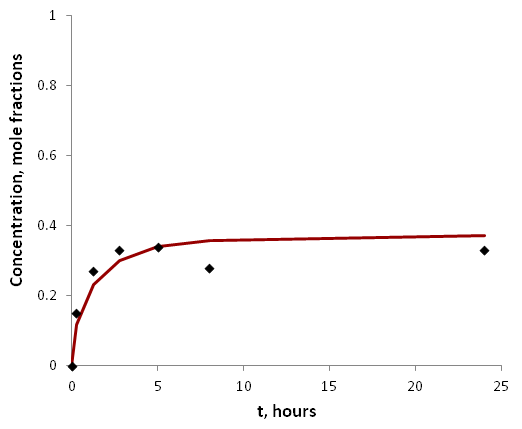
\includegraphics[width=1.0\linewidth]{figures/8_6b.png} \\ (b)}
\end{minipage}
\caption{The comparison of the calculated data with the experimental ones}
\label{8_fig_6}
\end{figure}


\section{Identification of the dynamic balance normative models of the regional economy}

In the present section, the results obtained within the research project supported by RFBR ``Parallel global optimization methods in the identification of the dynamic balance for the normative models of the regional economy'', project 11-07-97017, carried out jointly by the research teams from Lobachevsky State University of Nizhni Novgorod and from Dorodnicyn Computing Centre of RAS are presented \cite{8_Gergel2011}.

\subsection{Problem statement}

The regional economy (the district, region, or state, etc. level) was the object of investigations. For the mathematical description of the economical processes taking place at the regional level, a dynamic balance normative economic model has been proposed in Dorodnicyn Computing Centre of RAS \cite{8_Olenev1999}. This model is a general one. However, it includes a significant number of parameters  being specific to the different regions. It is possible to find these parameters (or \textit{to identify the model}) by solving the problem of minimization of the deviation of the calculated time series of the macroeconomic measures from the corresponding historic statistical data. The functions entering the problem statement are the nonlinear ones. As a result, the problem of identification of the mathematical economic model is the global optimization one.

Once the model was identified, it could be applied to verify various possible scenarios of the regional economic development on the base of the experiments with the model. The conclusions and predictions obtained using the identified mathematical model, in principle, could be disposed experimentally. This enables to correct further the model in order to obtain more justified prognosis based on the model being improved continuously. 

The problem of the identification of the multisector model of the regional economy presented here has been solved on the base of the data available for Nizhni Novgorod region, Russia. As it has been already mentioned above, the normative models include a large number of unknown parameters (the normatives of the distribution of the products and the normatives of distribution of the financial resources). In order to identify these parameters, it was proposed to apply the efficient parallel global optimization methods. The application of these algorithms on the supercomputer systems allows increasing the level of complexity of the mathematical models of the regional economy expressed by the number of the independent parameters. Carrying out the scenario computations based on the identified models of the regional economy allows more exact prognosis of the economic consequences of various strategic decisions.

\subsection{The description of the model of the regional economy}

The economy of Nizhni Novgorod region can be aggregated into three main sectors with approximately equal power:
\begin{itemize}
	\item the branches of the infrastructure, production and distribution of raw materials (agriculture, electric power industry, development, transportation, state administration, education, public health);
	\item the manufacturing branches (machine building and metal working, chemical and petrochemical industry, fuel industry, ferrous and nonferrous metallurgy, construction materials industry, timber, woodworking, and pulp-and-paper industry, consumer goods industry, food, pharmaceutical, chemical, microbiological industry, flour-and-cereals and feed mill industry, printing industry, scientific complex);
	\item the service branches (trading, operations with real estate, financial services, other services).
\end{itemize}

Let us select the following economic agents while designing the model: Regional Government, the producers represented by the three sectors selected above, the banking system, and the households of the region, the external vendors and consumers.

In spite of absence of rich natural resources in Nizhni Novgorod Region its economy is one of the most developed one with respect to the industry among the regions of Russian Federation. The processing branches of industry, a powerful military industrial complex, well-developed fundamental scientific complex are the base of the industry in Nizhni Novgorod Region and there are good prospects for the development of the high-tech industries and of the innovative branches.

The three-sector variant of the general balance model with supplies of products, factors of production, and financial resources in taxation and the illegal circulation of goods and finances \cite{8_Olenev2007} has been applied as the base for the design of the mathematical model of the regional economy. Remind that the producers in the model of Nizhni Novgorod Region economy are represented by three sectors: 
\begin{itemize}
	\item the infrastructure complex ($X$),
	\item the manufacturing branches complex ($Y$),
	\item the services, mortgage, financial, and trading branches complex ($Z$).
\end{itemize}
The producers (the sectors of the regional economy $X$, $Y$, $Z$) use labor, capital, and the intermediate production of the partner sectors. The producers deliver their products to the internal markets and to the external ones. The households $L$ offer the labor and consume the final products. The resellers $T$ redistribute the goods and financial flows. The banking system $B$ lends money to the producers with the purpose to receive the banking profit. Regional Government $G$ collects the taxes from the producers and the households and manages the budget expenditures. Each market is assumed to establish its own prices for each kind of products. The variations of the prices are assumed to be inversely proportional to the variation of the supplies of the corresponding products. 

In order to account for the illegal circulation of the goods and money, the producers were assumed to divide the manufactured products into the legal part and the illegal one. The latter does not undergo the taxation. As a result, the producers receive two kinds of income: the ``legal'' and the ``illegal'' one. The ``illegal'' money can be laundered and the reserves undergo penalties.

All the consumers’ money is assumed to be legal. The consumers’ income is assumed to be distributed between the acquisition of the legal products and the illegal ones from all sectors according to the predefined percentages. The production sectors $m = X,\;Y,\;Z$ pay the profit tax $n_1$, the value added tax $n_2$, the excise tax on the total output $n_3^m$ , the unified social tax on the payroll $n_4$, and the exports customs duties $n_5$. The households $L$ within the framework of the model pay the import customs duties $n_6$ and the income tax on the wages $n_7$.

The criteria and the parameters of the model have the upper and lower indices. The upper indices are used for the agents and the lower ones for the valuables. The supplies of each valuable are distributed according to the normative  $a_i^{nm}$, which are the portions of the amount of the valuable $i$ being transferred from the agent $n$ to the agent $m$. The distribution of money is also performed according to some normative $b_i^{nm}$, which are the portions of the money resources of the agent $m$ transferred to the agent $n$ for the product $i$. The capital coefficients are also defined by the normatives $c_i^m$ , which are the normalized amount of the product $i$ spent for the producing a unit of a fund product for the agent $m$.

The identification of the parameters was performed by the comparison of the output time series of the model variables with the available statistical time series in 2000--2008. As a criterion of proximity of the calculated time series to the statistical ones, Theil index was applied, which has been calculated according to the formula
\[
U=\frac{\sqrt{\sum{(x_i-y_i)^2}}}{\sqrt{\sum{x_i^2}}+\sqrt{\sum{y_i^2}}}
\]
The close the index to zero, the close the series compared.

\subsection{The results of the experiments}

The detailed description of the designed model is beyond the scope of this paper. The additional information can be found in \cite{8_Gergel2011}. Here we note that the global optimization problem arising in the model identification process has $60$ independent parameters, $86$ nonlinear constraints, and a multiextremal objective function. As an illustration, a two-dimensional section of the objective function confirming its essential multiextremality is presented in Fig.~\ref{8_fig_7}. 

\begin{figure}[t]
%\sidecaption[t]
\includegraphics[width=0.8\linewidth]{figures/8_7.png}
\caption{Two-dimensional section of the objective function}
\label{8_fig_7}     
\end{figure}

This problem has been solved on the cluster of Lobachevsky State University of Nizhni Novgorod using the parallel index method with the rotated evolvents (8 processors were employed). The estimate of optimum was obtained after $300 000$ iterations, the computation time of obtaining an estimate was $26$ minutes. Total computation time was $3$ hours.

Using the identified mathematical model of Nizhni Novgorod Region, the scenario computations reflecting the dynamics of the economic indicators of the region for various economic policies (the pessimistic scenario, the basic, and the optimistic one) have been carried out in Computing Centre of RAS.

\begin{thebibliography}{99.}

\bibitem{7_Gergel1993} 
Gergel, V.P.: A software system for multiextremal optimization. European Journal of Operational Research. \textbf{65(3)}, 305--313 (1993)

\bibitem{7_Pinter1996}
Pintér, J.D.: Global Optimization in Action (Continuous and Lipschitz Optimization: Algorithms, Implementations and Applications). Dordrecht: Kluwer Academic Publishers (1996)

\bibitem{7_Gergel2010}
Gergel, V.P., Labutina, A.A.: The ParaLab system for investigating the parallel algorithms. Lecture Notes in Computer Science. \textbf{6083}, 95--104 (2010)

\bibitem{8_Markine2005} 
Shevtsov, I.Y., Markine, V.L., Esveld, C.: Optimal design of wheel profile for railway vehicles. Wear. \textbf{258(7-8)}, 1022--1030 (2005)

\bibitem{8_Markine2007} 
Shevtsov, I.Y., Markine, V.L., Esveld, C.: An inverse shape design method for railway wheel profiles. Structural and Multidisciplinary Optimization. \textbf{33(3)}, 243--253 (2007)

\bibitem{8_Gubaidullin2011}
Gubaidullin, I.M., Ryabov, V.V., Tikhonova, M.V.: Application of the global optimization index method to solving inverse problems of chemical kinetics. Numerical methods and programming. \textbf{12(1)}, 137--145 (2011) (in Russian)

\bibitem{8_Gubaidullin2010}
Tikhonova, M.V., Gubaidullin, I.M., Spivak, S.I.: The numerical solution of the direct chemical kinetics problem by the Rosenbrock's and Mishelsen's methods for the stiff systems of differential equations. MVMS Journal. \textbf{12(12}, 26--33 (2010) (in Russian)

\bibitem{8_Parfenova2009}
Parfenova, L.V., Gabdrakhmanov, V.Z., Khalilov, L.M., Dzhemilev, U.M.: On study of chemoselectivity of reaction of trialkylalanes with alkenes, catalyzed with $Zr$ $\pi$-complexes. Journal of Organometallic Chemistry. \textbf{694(23)}, 3725--3731 (2009)

\bibitem{8_Gergel2011}
Gergel, V.P., Gorbachev, V.A., Olenev, N.N., Ryabov, V.V., Sidorov, S.V. Parallel global optimization methods for identification of the dynamic balance normative model of regional economy. Bulletin of South Ural State University. \textbf{25(9)}, 4--15 (2011) (In Russian)

\bibitem{8_Olenev1999}
Avtukhovich, E.V., Guriev, S.M., Olenev, N.N., Petrov, A.A., Pospelov, I.G., Shananin, A.A., Chukanov, S.V.: A Mathematical Model of the Transition Economy. The Computing Centre of the Russian Academy of Sciences, Moscow (1999) (In Russian)

\bibitem{8_Olenev2007}
Olenev, N.N.: Model of innovation potential of regional economy. Proceedings of international conference ``Economy of depressed areas: problems and prospects of progress of regional economy''. Altai State University Press. 178--188 (2007) (In Russian)

\end{thebibliography}

%\end{document}

%%%%%%%%%%%%%%%%%%%% author.tex %%%%%%%%%%%%%%%%%%%%%%%%%%%%%%%%%%%
%
% sample root file for your "contribution" to a contributed volume
%
% Use this file as a template for your own input.
%
%%%%%%%%%%%%%%%% Springer %%%%%%%%%%%%%%%%%%%%%%%%%%%%%%%%%%%%%%%%%


%%% RECOMMENDED %%%%%%%%%%%%%%%%%%%%%%%%%%%%%%%%%%%%%%%%%%%%%%%%%%%
%\documentclass[graybox]{svmult}
%%
%%% choose options for [] as required from the list
%%% in the Reference Guide
%%
%\usepackage{mathptmx}       % selects Times Roman as basic font
%\usepackage{helvet}         % selects Helvetica as sans-serif font
%\usepackage{courier}        % selects Courier as typewriter font
%%\usepackage{type1cm}        % activate if the above 3 fonts are
                             %% not available on your system
%%
%\usepackage{makeidx}         % allows index generation
%\usepackage{graphicx}        % standard LaTeX graphics tool
%%                             % when including figure files
%\usepackage{multicol}        % used for the two-column index
%\usepackage[bottom]{footmisc}% places footnotes at page bottom
%
%
%\usepackage[colorlinks=true]{hyperref}
%%\hypersetup{urlcolor=blue, citecolor=red}
%

%% see the list of further useful packages
%% in the Reference Guide
%
%\makeindex             % used for the subject index
%                       % please use the style svind.ist with
%                       % your makeindex program
%
%%%%%%%%%%%%%%%%%%%%%%%%%%%%%%%%%%%%%%%%%%%%%%%%%%%%%%%%%%%%%%%%%%%%%%%%%%%%%%%%%%%%%%%%%%
%
%\begin{document}

\title{Supercomputer parallel computations in solving the applied optimization problems }
% Use \titlerunning{Short Title} for an abbreviated version of
% your contribution title if the original one is too long
\author{Konstantin Barkalov}
% Use \authorrunning{Short Title} for an abbreviated version of
% your contribution title if the original one is too long
\institute{Konstantin Barkalov \at Lobachevsky State University of Nizhni Novgorod,  Nizhni Novgorod, Russia \email{konstantin.barkalov@itmm.unn.ru}}
%
% Use the package "url.sty" to avoid
% problems with special characters
% used in your e-mail or web address
%
\maketitle

\abstract*{In this paper, the examples of solving the applied problems in the fields of optimal design (the finding of the optimum profile of a vehicle wheel), chemical research (finding the unknown kinetic parameters in the mathematical models of the complex chemical reactions), economics (the identification of the parameters in the regional economic model) are given.}

\abstract{In this paper, the examples of solving the applied problems in the fields of optimal design (the finding of the optimum profile of a vehicle wheel), chemical research (finding the unknown kinetic parameters in the mathematical models of the complex chemical reactions), economics (the identification of the parameters in the regional economic model) are given.}

\section{Optimization of the rail transport wheel profile}

The considered problem of the search for the optimum profile of the wheels for the rail transport (railway, subway, tram, etc.) has been solved in the framework of joint research project supported by Russian Foundation for Basic Research (project number 04-01-89002-NVO\_a) and NWO (Netherlands Organization for Scientific Research, project number 047.016.014)  ``Fast Computing in Global Optimization: Sequential and Parallel Environments'', carried out at Lobachevsky State University of Nizhni Novgorod and Delft University of Technology, the Netherlands (TU Delft).

\subsection{Problem Statement}

The problem of the rail transport wheel profile optimization is described in details in \cite{8_Markine2005,8_Markine2007}. Here, a brief description of this problem is presented only. Since the wheels are of the conical shape, the center of a mounted axle is moving along a sinusoid. This process is illustrated in Fig.~\ref{8_fig_1}). The parameters of the contact between the wheel and the rail, such as the radius of rotation, the contact angle, and the angle of inclination for the mounted axle are varied at the transverse displacement of the mounted axle relative to the rail. The relationship between these variations and the transverse position of the mounted axle is determined by the wheel and rail profiles.

\begin{figure}[t]
%\sidecaption[t]
\includegraphics[width=0.9\linewidth]{figures/8_1.png}
\caption{The displacement of the mounted axle}
\label{8_fig_1}     
\end{figure}

The radius of rotation of the wheel at the contact point is an important parameter of the contact between the wheel and the rail. Actually, the radius can be different for the right and the left wheels since the mounted axle can shift relative to the rail (the radii $r_1$ and $r_2$, respectively in Fig.~\ref{8_fig_2}).

\begin{figure}[t]
%\sidecaption[t]
\includegraphics[width=0.7\linewidth]{figures/8_2.png}
\caption{The difference in the radii of rotation}
\label{8_fig_2}     
\end{figure}

When the mounted axle is in the central position, the radii of rotation are the same for the left and right wheels, i.e., $r_1=r_2=r$. The difference in the radii of rotation for the left and right wheels can be defined as a function of the transverse displacement of the mounted axle relative to its central position $\Delta r(x)=r_1(x)-r_2(x)$.

The mathematical model for this problem developed in Technical University Delft consists in the following. The wheel profile is described by B-spline, for building of which a set of points on the edge, on the edge base, and on the rolling surface of the wheel were selected (Fig.~\ref{8_fig_3})). Positions of these points can be varied for the purpose of variation of the profile. In order to reduce the computational costs for the optimization, the positions of the points on the upper surface of the edge as well as on the conical part of the profile were fixed since these parts of the wheel profile do not contact the rails.

\begin{figure}[t]
%\sidecaption[t]
\includegraphics[width=0.7\linewidth]{figures/8_3.png}
\caption{Modeling of the wheel profile}
\label{8_fig_3}     
\end{figure}

The ordinates of the movable points of the spline $z_i$ were selected as the components of the vector of the optimization problem parameters $y$, i.e.,
\[
y=(z_1,...,z_N),
\]
and the abscissas of these points were fixed.

The number of the movable points and, consequently, the number $N$ of variables in the considered problem was equal to $11$. For each parameter   the interval $\left[–1, 1\right]$ was taken as the domain of its variation. The difference of the radii of rotation $\Delta r(x)$ was minimized. The constraints were introduced according to the stability considerations. For example, one of the constraints was imposed on the maximum angle of inclination for the mounted axle.

\subsection{The results of the experiments}

Thus, the optimization problem has $N=11$ parameters and $m=6$ constraints. The objective function as well as the constraint functions is the multiextremal ones. A one-dimensional section of the objective function is presented in Fig.~\ref{8_fig_4} for illustration.

\begin{figure}[t]
%\sidecaption[t]
\includegraphics[width=0.7\linewidth]{figures/8_4.png}
\caption{A section of the objective function }
\label{8_fig_4}     
\end{figure}

The constraints have no analytical form and defined by a MATLAB computational procedures. The computation of the values of all problem functions (objective function and constraints) at one point $y$ using Pentium IV processor with the clock frequency of 3 GHz takes about 10 sec. 

Thus, having formulated the problem, let us try to estimate the resources required for its solving in dependence on the method selected. Let us take, for example, the method of full scanning a uniform grid. Having selected 10 variants for the values of each parameter (remind, that the total number of parameters equals to 11), we obtain $10^{11}$ computations at the grid nodes that requires $\sim 10^{12}$ sec., i.e., $\sim 3$ years of computations using a supercomputer with 10 000 processors. Thus, the problem is so hard to solve that the parallel computations are not only necessary but should be supplied with the efficient numerical methods to obtain the results in a reasonable time unavoidably.

The problem described above has been solved by the authors using the parallel index method with the multiple shifted evolvents on a cluster of 4 computers in Delft University of Technology. The search precision in the coordinates was $2^{-10}$ , i.e., 1024 points of each parameter value in the case of the full scanning method. The search time for the optimum estimate was 27 hours. The problem functions values have been computed $4297 + 4415 + 4236 + 4266 = 17214$ times.

The computations carried out at TU Delft for a wheel of the optimum profile demonstrated its service life to increase up to 120 000 km between the profile corrections (more than five times longer as compared to the wheels of the original profile) and the maximum permitted speed to increase from 40 up to 60 m/sec.

\section{Solving the inverse problem of chemical kinetics}

In the present section the results of joint research project carried out at Lobachevsky State University of Nizhni Novgorod and at Institute of Petrochemistry and Catalysis, Russian Academy of Sciences (IPC RAS) \cite{8_Gubaidullin2011}.

\subsection{Problem statement}

The building of the mathematical models of the complex chemical reactions implies the presence of the unknown kinetic parameters (the rate constants, the activation energies, and the frequencies of collisions between the reacting molecules), which could be found by solving the problem of the minimization of the deviations between the calculated data (\textit{the direct problem}) and the experimental ones. Thus, a problem of identifying the mathematical model (\textit{the inverse problem of chemical kinetics}) arises, which in general case is a global optimization problem.

Many problems of physics chemistry imply a considerable amount of computations, nevertheless, providing rather low precision. Investigating the inverse problems of chemical kinetics requires solving many systems of differential and algebraic equations. The kinetics of complex chemical reactions is featured by the presence of parameters varying fast and slowly (because various stages of reactions go with different rates). Therefore, solving the direct kinetic problems is complicated by the hardness of the differential equations describing the mechanisms of these reactions.

The direct kinetic problem for the isothermal non-stationary model in a closed system is Cauchy problem for a system of ordinary differential equations
\begin{equation} 
 \frac{dx_i}{dt}= F_i, i=1,..,M; \; F_i=\sum_{j=1}^{N}{S_{ij}w_j}
\end{equation}
\begin{equation} 
 w_j=k_j\prod_{i=1}^{M}{\left(x_i\right)^{\left|\alpha_{ij}\right|}}-k_{-j}\prod_{i=1}^{M}{\left(x_i\right)^{\left|\beta_{ij}\right|}}
\end{equation}
with the initial conditions $t=0$, $x_i(0)=x_i^0$, where 
\begin{itemize}
	\item $x_i$ are the concentrations of the substances (\textit{the molar fractions}) participating in the reaction;
	\item $M$ is the number of substances; 
	\item $N$ is the number of steps;
	\item $S_{ij}$ are the stoichiometric matrix; 
	\item $w_j$ are the rates of the $j$-th step, $1/{hr}$; 
	\item $k_j$, $k_{-j}$ are the reduced rate constants for the forward and reverse reactions ($1/{hr}$), respectively;
	\item $\alpha_{ij}$ are the negative elements of $S_{ij}$, and $\beta_{ij}$ are the positive elements of $S_{ij}$.
\end{itemize}

Since a part of the constants $k_j$, $k_{-j}$, as a rule, are not known, the problem of identification of the mathematical model of  the inverse kinetic problem arises. This problem is a minimization one for the function of the deviation between the calculated data and the experimental ones
\begin{equation} \label{8_chem_func}
F=\sum_{i=1}^n{\sum_{j=1}^M{\left|x_{ij}^p-x_{ij}^{\epsilon}\right|}}\rightarrow \min,
\end{equation}
where
\begin{itemize}
	\item $x_{ij}^p$ are the calculated values of the observable substances concentrations  (\textit{molar fractions});	
	\item $x_{ij}^{\epsilon}$ are the values of the observable substances concentrations measured experimentally (\textit{molar fractions});
	\item $n$ is the number of the experimental points.
\end{itemize}

To find the activation energies and the collision frequencies of the molecules reacting at the elementary step, Arrhenius equation
\[
k=Ae^{-\frac{Ea}{RT}}
\]
is used, where
\begin{itemize}
	\item $k$ is the reduced rate constant for the elementary step, $1/hr$;	
	\item $E$ is the activation energy, $J/{mol}$;
	\item $R$ is gas constant, $J/{(mol \cdot K)}$;
	\item $А$ is the collision frequency for the reacting molecules;
	\item $T$ is the temperature, $K$.	
\end{itemize}

Since in the search for the rate constants of the elementary steps, these ones may fall into the area, where the differential equations system describing the reactions may appear to be a stiff one, Mishelsen method with automatic step selection is applied to solving the direct problem \cite{8_Gubaidullin2010}. As the model output data $x_{ij}^p$ depend on the values of the constants $k_j$, $k_{-j}$ nonlinearly, problem (\ref{8_chem_func}) is a multiextremal optimization problem.

\subsection{The results of the experiments}

Traditionally, the methods based on the random search ideas had been applied in IPC RAS for solving problem (\ref{8_chem_func}). The typical computation costs were several days of continuous computations. Within the framework of the joint research project by IPC RAS and Lobachevsky State University of Nizhni Novgorod it was proposed to apply the efficient parallel global optimization methods developed in UNN. 

For the application of the novel identification technique the mathematical model for the reaction of the catalytical carboalumination of olefins and acetylenes with the assistance of threealkylalanes in the presence of transition metal complexes was selected. This reaction has applied in the laboratory research at IPC RAS as an efficient method for the synthesis of new Me-C (methyl-carbon), Et-C (ethyl-carbon), and C-C (carbon-carbon) bonds \cite{8_Parfenova2009}. The natural experiments of conducting the reactions of the catalytical carboalumination of olefins and acetylenes for different temperatures and fixed initial concentrations have been carried out in IPC RAS. In the experiments, the concentrations of five substances were traced and their percentage ratios were determined. A number of schemes for the mathematical description of the reaction of catalytical carboalumination of olefins and acetylenes (including the parameters to be identified) have been proposed in IPC RAS. As a priority problem of the identification of the unknown parameters, it was required to determine the rate constants for the elementary steps for the proposed reaction schemes for various temperatures as well as to find the activation energies for the elementary steps for various catalysts. These schemes and the identification problem have been described in details in \cite{8_Gubaidullin2011}. Here, note that the minimization problem arising depends on 10 parameters and is box-constrained one. The computational costs for the function value at one point are $\sim 3$ sec. (Intel Xeon 3.2 GHz). The objective function is  multiextremal that is confirmed by its two-dimensional section presented in Fig.~\ref{8_fig_5}. 

\begin{figure}[t]
%\sidecaption[t]
\includegraphics[width=0.8\linewidth]{figures/8_5.png}
\caption{Two-dimensional section of the objective function}
\label{8_fig_5}     
\end{figure}

As a result of the computations, the estimates of the rate constants for the elementary steps for the 10- and 12-step reactions schemes of the carboalumination in the presence of $Cp_2 ZrCl_2$ catalyst have been obtained. The objective function value at the obtained optimizer was $F = 3.040$. It appeared to be impossible to achieve the function value close to zero because the experimental data contains the uncertainties. Nevertheless, the model identified using the parallel global optimization method allowed obtaining a good conformity between the calculated data and the experimental ones. As an illustration, the comparison of the computed and experimental concentrations of substances participating in the reactions is presented in Fig.~\ref{8_fig_6}.

\begin{figure}
\begin{minipage}{0.5\linewidth}
\center{\includegraphics[width=1.0\linewidth]{figures/8_6a.png} \\ (a)}
\end{minipage}
\hfill
\begin{minipage}{0.5\linewidth}
\center{\includegraphics[width=1.0\linewidth]{figures/8_6b.png} \\ (b)}
\end{minipage}
\caption{The comparison of the calculated data with the experimental ones}
\label{8_fig_6}
\end{figure}


\section{Identification of the dynamic balance normative models of the regional economy}

In the present section, the results obtained within the research project supported by RFBR ``Parallel global optimization methods in the identification of the dynamic balance for the normative models of the regional economy'', project 11-07-97017, carried out jointly by the research teams from Lobachevsky State University of Nizhni Novgorod and from Dorodnicyn Computing Centre of RAS are presented \cite{8_Gergel2011}.

\subsection{Problem statement}

The regional economy (the district, region, or state, etc. level) was the object of investigations. For the mathematical description of the economical processes taking place at the regional level, a dynamic balance normative economic model has been proposed in Dorodnicyn Computing Centre of RAS \cite{8_Olenev1999}. This model is a general one. However, it includes a significant number of parameters  being specific to the different regions. It is possible to find these parameters (or \textit{to identify the model}) by solving the problem of minimization of the deviation of the calculated time series of the macroeconomic measures from the corresponding historic statistical data. The functions entering the problem statement are the nonlinear ones. As a result, the problem of identification of the mathematical economic model is the global optimization one.

Once the model was identified, it could be applied to verify various possible scenarios of the regional economic development on the base of the experiments with the model. The conclusions and predictions obtained using the identified mathematical model, in principle, could be disposed experimentally. This enables to correct further the model in order to obtain more justified prognosis based on the model being improved continuously. 

The problem of the identification of the multisector model of the regional economy presented here has been solved on the base of the data available for Nizhni Novgorod region, Russia. As it has been already mentioned above, the normative models include a large number of unknown parameters (the normatives of the distribution of the products and the normatives of distribution of the financial resources). In order to identify these parameters, it was proposed to apply the efficient parallel global optimization methods. The application of these algorithms on the supercomputer systems allows increasing the level of complexity of the mathematical models of the regional economy expressed by the number of the independent parameters. Carrying out the scenario computations based on the identified models of the regional economy allows more exact prognosis of the economic consequences of various strategic decisions.

\subsection{The description of the model of the regional economy}

The economy of Nizhni Novgorod region can be aggregated into three main sectors with approximately equal power:
\begin{itemize}
	\item the branches of the infrastructure, production and distribution of raw materials (agriculture, electric power industry, development, transportation, state administration, education, public health);
	\item the manufacturing branches (machine building and metal working, chemical and petrochemical industry, fuel industry, ferrous and nonferrous metallurgy, construction materials industry, timber, woodworking, and pulp-and-paper industry, consumer goods industry, food, pharmaceutical, chemical, microbiological industry, flour-and-cereals and feed mill industry, printing industry, scientific complex);
	\item the service branches (trading, operations with real estate, financial services, other services).
\end{itemize}

Let us select the following economic agents while designing the model: Regional Government, the producers represented by the three sectors selected above, the banking system, and the households of the region, the external vendors and consumers.

In spite of absence of rich natural resources in Nizhni Novgorod Region its economy is one of the most developed one with respect to the industry among the regions of Russian Federation. The processing branches of industry, a powerful military industrial complex, well-developed fundamental scientific complex are the base of the industry in Nizhni Novgorod Region and there are good prospects for the development of the high-tech industries and of the innovative branches.

The three-sector variant of the general balance model with supplies of products, factors of production, and financial resources in taxation and the illegal circulation of goods and finances \cite{8_Olenev2007} has been applied as the base for the design of the mathematical model of the regional economy. Remind that the producers in the model of Nizhni Novgorod Region economy are represented by three sectors: 
\begin{itemize}
	\item the infrastructure complex ($X$),
	\item the manufacturing branches complex ($Y$),
	\item the services, mortgage, financial, and trading branches complex ($Z$).
\end{itemize}
The producers (the sectors of the regional economy $X$, $Y$, $Z$) use labor, capital, and the intermediate production of the partner sectors. The producers deliver their products to the internal markets and to the external ones. The households $L$ offer the labor and consume the final products. The resellers $T$ redistribute the goods and financial flows. The banking system $B$ lends money to the producers with the purpose to receive the banking profit. Regional Government $G$ collects the taxes from the producers and the households and manages the budget expenditures. Each market is assumed to establish its own prices for each kind of products. The variations of the prices are assumed to be inversely proportional to the variation of the supplies of the corresponding products. 

In order to account for the illegal circulation of the goods and money, the producers were assumed to divide the manufactured products into the legal part and the illegal one. The latter does not undergo the taxation. As a result, the producers receive two kinds of income: the ``legal'' and the ``illegal'' one. The ``illegal'' money can be laundered and the reserves undergo penalties.

All the consumers’ money is assumed to be legal. The consumers’ income is assumed to be distributed between the acquisition of the legal products and the illegal ones from all sectors according to the predefined percentages. The production sectors $m = X,\;Y,\;Z$ pay the profit tax $n_1$, the value added tax $n_2$, the excise tax on the total output $n_3^m$ , the unified social tax on the payroll $n_4$, and the exports customs duties $n_5$. The households $L$ within the framework of the model pay the import customs duties $n_6$ and the income tax on the wages $n_7$.

The criteria and the parameters of the model have the upper and lower indices. The upper indices are used for the agents and the lower ones for the valuables. The supplies of each valuable are distributed according to the normative  $a_i^{nm}$, which are the portions of the amount of the valuable $i$ being transferred from the agent $n$ to the agent $m$. The distribution of money is also performed according to some normative $b_i^{nm}$, which are the portions of the money resources of the agent $m$ transferred to the agent $n$ for the product $i$. The capital coefficients are also defined by the normatives $c_i^m$ , which are the normalized amount of the product $i$ spent for the producing a unit of a fund product for the agent $m$.

The identification of the parameters was performed by the comparison of the output time series of the model variables with the available statistical time series in 2000--2008. As a criterion of proximity of the calculated time series to the statistical ones, Theil index was applied, which has been calculated according to the formula
\[
U=\frac{\sqrt{\sum{(x_i-y_i)^2}}}{\sqrt{\sum{x_i^2}}+\sqrt{\sum{y_i^2}}}
\]
The close the index to zero, the close the series compared.

\subsection{The results of the experiments}

The detailed description of the designed model is beyond the scope of this paper. The additional information can be found in \cite{8_Gergel2011}. Here we note that the global optimization problem arising in the model identification process has $60$ independent parameters, $86$ nonlinear constraints, and a multiextremal objective function. As an illustration, a two-dimensional section of the objective function confirming its essential multiextremality is presented in Fig.~\ref{8_fig_7}. 

\begin{figure}[t]
%\sidecaption[t]
\includegraphics[width=0.8\linewidth]{figures/8_7.png}
\caption{Two-dimensional section of the objective function}
\label{8_fig_7}     
\end{figure}

This problem has been solved on the cluster of Lobachevsky State University of Nizhni Novgorod using the parallel index method with the rotated evolvents (8 processors were employed). The estimate of optimum was obtained after $300 000$ iterations, the computation time of obtaining an estimate was $26$ minutes. Total computation time was $3$ hours.

Using the identified mathematical model of Nizhni Novgorod Region, the scenario computations reflecting the dynamics of the economic indicators of the region for various economic policies (the pessimistic scenario, the basic, and the optimistic one) have been carried out in Computing Centre of RAS.

\begin{thebibliography}{99.}

\bibitem{8_Markine2005} 
Shevtsov, I.Y., Markine, V.L., Esveld, C.: Optimal design of wheel profile for railway vehicles. Wear. \textbf{258(7-8)}, 1022--1030 (2005)

\bibitem{8_Markine2007} 
Shevtsov, I.Y., Markine, V.L., Esveld, C.: An inverse shape design method for railway wheel profiles. Structural and Multidisciplinary Optimization. \textbf{33(3)}, 243--253 (2007)

\bibitem{8_Gubaidullin2011}
Gubaidullin, I.M., Ryabov, V.V., Tikhonova, M.V.: Application of the global optimization index method to solving inverse problems of chemical kinetics. Numerical methods and programming. \textbf{12(1)}, 137--145 (2011) (in Russian)

\bibitem{8_Gubaidullin2010}
Tikhonova, M.V., Gubaidullin, I.M., Spivak, S.I.: The numerical solution of the direct chemical kinetics problem by the Rosenbrock's and Mishelsen's methods for the stiff systems of differential equations. MVMS Journal. \textbf{12(12}, 26--33 (2010) (in Russian)

\bibitem{8_Parfenova2009}
Parfenova, L.V., Gabdrakhmanov, V.Z., Khalilov, L.M., Dzhemilev, U.M.: On study of chemoselectivity of reaction of trialkylalanes with alkenes, catalyzed with $Zr$ $\pi$-complexes. Journal of Organometallic Chemistry. \textbf{694(23)}, 3725--3731 (2009)

\bibitem{8_Gergel2011}
Gergel, V.P., Gorbachev, V.A., Olenev, N.N., Ryabov, V.V., Sidorov, S.V. Parallel global optimization methods for identification of the dynamic balance normative model of regional economy. Bulletin of South Ural State University. \textbf{25(9)}, 4--15 (2011) (In Russian)

\bibitem{8_Olenev1999}
Avtukhovich, E.V., Guriev, S.M., Olenev, N.N., Petrov, A.A., Pospelov, I.G., Shananin, A.A., Chukanov, S.V.: A Mathematical Model of the Transition Economy. The Computing Centre of the Russian Academy of Sciences, Moscow (1999) (In Russian)

\bibitem{8_Olenev2007}
Olenev, N.N.: Model of innovation potential of regional economy. Proceedings of international conference ``Economy of depressed areas: problems and prospects of progress of regional economy''. Altai State University Press. 178--188 (2007) (In Russian)




\end{thebibliography}

%\end{document}

%

\backmatter%%%%%%%%%%%%%%%%%%%%%%%%%%%%%%%%%%%%%%%%%%%%%%%%%%%%%%%
\appendix
%%%%%%%%%%%%%%%%%%%%% appendix.tex %%%%%%%%%%%%%%%%%%%%%%%%%%%%%%%%%
%
% sample appendix
%
% Use this file as a template for your own input.
%
%%%%%%%%%%%%%%%%%%%%%%%% Springer-Verlag %%%%%%%%%%%%%%%%%%%%%%%%%%

\chapter{Chapter Heading}
\label{introA} % Always give a unique label
% use \chaptermark{}
% to alter or adjust the chapter heading in the running head

Use the template \emph{appendix.tex} together with the Springer document class SVMono (monograph-type books) or SVMult (edited books) to style appendix of your book in the Springer layout.


\section{Section Heading}
\label{sec:A1}
% Always give a unique label
% and use \ref{<label>} for cross-references
% and \cite{<label>} for bibliographic references
% use \sectionmark{}
% to alter or adjust the section heading in the running head
Instead of simply listing headings of different levels we recommend to let every heading be followed by at least a short passage of text. Further on please use the \LaTeX\ automatism for all your cross-references and citations.


\subsection{Subsection Heading}
\label{sec:A2}
Instead of simply listing headings of different levels we recommend to let every heading be followed by at least a short passage of text. Further on please use the \LaTeX\ automatism for all your cross-references and citations as has already been described in Sect.~\ref{sec:A1}.

For multiline equations we recommend to use the \verb|eqnarray| environment.
\begin{eqnarray}
\vec{a}\times\vec{b}=\vec{c} \nonumber\\
\vec{a}\times\vec{b}=\vec{c}
\label{eq:A01}
\end{eqnarray}

\subsubsection{Subsubsection Heading}
Instead of simply listing headings of different levels we recommend to let every heading be followed by at least a short passage of text. Further on please use the \LaTeX\ automatism for all your cross-references and citations as has already been described in Sect.~\ref{sec:A2}.

Please note that the first line of text that follows a heading is not indented, whereas the first lines of all subsequent paragraphs are.

% For figures use
%
%\begin{figure}[t]
%\sidecaption[t]
%% Use the relevant command for your figure-insertion program
%% to insert the figure file.
%% For example, with the graphicx style use
%\includegraphics[scale=.65]{figure}
%%
%% If no graphics program available, insert a blank space i.e. use
%%\picplace{5cm}{2cm} % Give the correct figure height and width in cm
%%
%\caption{Please write your figure caption here}
%\label{fig:A1}       % Give a unique label
%\end{figure}

% For tables use
%
\begin{table}
\caption{Please write your table caption here}
\label{tab:A1}       % Give a unique label
%
% Follow this input for your own table layout
%
\begin{tabular}{p{2cm}p{2.4cm}p{2cm}p{4.9cm}}
\hline\noalign{\smallskip}
Classes & Subclass & Length & Action Mechanism  \\
\noalign{\smallskip}\hline\noalign{\smallskip}
Translation & mRNA$^a$  & 22 (19--25) & Translation repression, mRNA cleavage\\
Translation & mRNA cleavage & 21 & mRNA cleavage\\
Translation & mRNA  & 21--22 & mRNA cleavage\\
Translation & mRNA  & 24--26 & Histone and DNA Modification\\
\noalign{\smallskip}\hline\noalign{\smallskip}
\end{tabular}
$^a$ Table foot note (with superscript)
\end{table}
%

%%%%%%%%%%%%%%%%%%%%%%acronym.tex%%%%%%%%%%%%%%%%%%%%%%%%%%%%%%%%%%%%%%%%%
% sample list of acronyms
%
% Use this file as a template for your own input.
%
%%%%%%%%%%%%%%%%%%%%%%%% Springer %%%%%%%%%%%%%%%%%%%%%%%%%%

\Extrachap{Glossary}


Use the template \emph{glossary.tex} together with the Springer document class SVMono (monograph-type books) or SVMult (edited books) to style your glossary\index{glossary} in the Springer layout.


\runinhead{glossary term} Write here the description of the glossary term. Write here the description of the glossary term. Write here the description of the glossary term.

\runinhead{glossary term} Write here the description of the glossary term. Write here the description of the glossary term. Write here the description of the glossary term.

\runinhead{glossary term} Write here the description of the glossary term. Write here the description of the glossary term. Write here the description of the glossary term.

\runinhead{glossary term} Write here the description of the glossary term. Write here the description of the glossary term. Write here the description of the glossary term.

\runinhead{glossary term} Write here the description of the glossary term. Write here the description of the glossary term. Write here the description of the glossary term.
\printindex

%%%%%%%%%%%%%%%%%%%%%%%%%%%%%%%%%%%%%%%%%%%%%%%%%%%%%%%%%%%%%%%%%%%%%%

\end{document}
